\documentclass[a4paper,12pt,titlepage, onecolumn, twoside]{report}
\usepackage[english,brazilian]{babel} % suporte para línguas
\usepackage[utf8]{inputenc} % codificação


\usepackage{subfig, epsfig}
\captionsetup[subfigure]{style=default, 
  margin=0pt, parskip=0pt, hangindent=0pt, indention=0pt, 
  singlelinecheck=true, labelformat=parens, labelsep=space}

\usepackage{ae}
\usepackage{aecompl}
\usepackage{booktabs}
\usepackage[T1] {fontenc}
\usepackage{lmodern} %test

\usepackage{footnote}
\usepackage{geometry}
\geometry{includeheadfoot,verbose,tmargin=2.7cm,bmargin=2.9cm}
%originally bmargin=3.7 and tmargin=2.8
\usepackage{fancyhdr}
\usepackage{afterpage}

\usepackage[table,xcdraw]{xcolor}

\usepackage{multirow}
\usepackage{csquotes}
\usepackage{placeins}


% Notas criadas nas tabelas ficam no fim das tabelas
\makesavenoteenv{tabular}
\usepackage{longtable}

\pagestyle{fancy}

%\fancypagestyle{plain}
%{
%  \fancyhf{}%
%  \renewcommand{\headrulewidth}{0pt}%
%  \fancyfoot[C]{\thepage}
%}

\usepackage{xr}
\usepackage{graphicx,wrapfig} % para incluir figuras
\usepackage[all]{xy} % para incluir diagramas
\usepackage{amsfonts, amssymb, amsthm, amsmath, amscd, textcomp} % pacote AMS

\usepackage{color, float, bbm, multicol, rotating}
\usepackage{verbatim, listings, booktabs}


\usepackage{caption} % Customizar as legendas de figuras e tabelas
\usepackage{array} % Elementos extras para formatação de tabelas

\usepackage[switch*,pagewise]{lineno} % números nas linhas

\renewcommand{\thefigure}{\arabic{figure}}
\renewcommand{\thetable}{\arabic{table}}

\extrafloats{100}
\usepackage[maxfloats=50]{morefloats}

\usepackage {tocvsec2} % controlar profundidade de table of contents
\setcounter {secnumdepth}{0}
\setcounter {tocdepth}{2}

%\widowpenalty10000
%\clubpenalty10000

\usepackage{mathpazo} % fonte palatino
\usepackage{hyperref}
\usepackage[numbered]{bookmark} %test

% Adicionar bibliografia, índice e conteúdo na Tabela de conteúdo
% Não inclui lista de tabelas e figuras no índice
\usepackage[nottoc,notlof,notlot, notindex]{tocbibind}

\usepackage{icomma} % Posicionar inteligentemente a vírgula como separador decimal
\usepackage[tight]{units} % Formatar as unidades com as distâncias corretas

\usepackage{setspace}

\usepackage{lastpage} % Conta o número de páginas
%\usepackage{pageslts} %test
\usepackage{pdflscape} % ambiente landscape

%\usepackage[round]{natbib}
 
%\usepackage[sectionbib, round]{natbib}
%\usepackage{chapterbib}
%\bibliographystyle{disertacao}


\usepackage[firstinits=true,
			uniquename=false,
            uniquelist=false,
            sorting=anyt,
			url=true,
            doi=false,
            isbn=true,
            maxcitenames=2,
            mincitenames=1,
            maxbibnames=10,
            bibencoding=inputenc,
            hyperref=auto,
            style=authoryear,            
            refsection=chapter]
{biblatex}
%add parenthesis in volume/issue in references
\renewbibmacro*{volume+number+eid}{%
  \printfield{volume}%
%  \setunit*{\adddot}% DELETED
  \setunit*{\addnbspace}% NEW (optional); there's also \addnbthinspace
  \printfield{number}%
  \setunit{\addcomma\space}%
  \printfield{eid}}
\DeclareFieldFormat[article]{number}{\mkbibparens{#1}}

%add comma between author and year
\renewcommand*{\nameyeardelim}{\addcomma\space}

\AtEveryBibitem{\ifentrytype{article}{\clearfield{issn}}{}} %do not print ISSN for articles

\AtEveryBibitem{\ifentrytype{article}{\clearfield{url}}{}} %do not print URL unless it is a thesis.

\bibliography{Thesis}



\usepackage[flushleft]{threeparttable}
\usepackage{tabularx}

\usepackage{pdfpages}

\usepackage{fixme}
%\usepackage{pdfcomment}

\fxsetup{layout={footnote}}

\usepackage{titlesec}
\usepackage{etoolbox}
\usepackage{chngcntr}
\counterwithout{equation}{chapter}
\usepackage{lineno}

\usepackage{lettrine} %fancy big letter

\usepackage{epstopdf}
\epstopdfDeclareGraphicsRule{.tiff}{png}{.png}{convert #1 \OutputFile}
\AppendGraphicsExtensions{.tiff}  %convert tiff images tp PNG

% --- definições gerais ---
\newcommand{\barra}{\backslash}
\newcommand{\To}{\longrightarrow}
\newcommand{\abs}[1]{\left\vert#1\right\vert}
\newcommand{\set}[1]{\left\{#1\right\}}
\newcommand{\seq}[1]{\left<#1\right>}
\newcommand{\norma}[1]{\left\Vert#1\right\Vert}
\newcommand{\hr}{\par\noindent\hrulefill\par}
\definecolor{airforceblue}{rgb}{0.36, 0.54, 0.66}
%\preto\chapter{\color{airforceblue}}
%\titleformat{\chapter}[hang]{\Huge\bfseries}{\thechapter\hsp\textcolor{gray75}{|}\hsp}{0pt}{\Huge\bfseries}
% --- ---


%\newcommand{\titulo}{Má-adaptação como subproduto da adaptação: um estudo em escala genômica}
%\newcommand{\nomedoaluno}{Bárbara Domingues Bitarello}
%\newcommand{\advisor}{Diogo Meyer} \newcommand{\ano}{2015}
%\hypersetup{colorlinks=true, linkcolor=black, citecolor=black,
%  filecolor=black, pagecolor=black, urlcolor=black,
%  pdfauthor={\nomedoaluno}, pdftitle={\titulo}, pdfsubject={Genética e
%    Biologia Evolutiva}, pdfkeywords={Genética Quantitiva, Morfologia
%    Craniana, Roedores}, pdfproducer={Latex}, pdfcreator={pdflatex}}
 
%\geometry{bindingoffset=20pt}
%\geometry{paperwidth=290mm, paperheight=297mm, margin=1in}
%\setlength{\marginparwidth=80mm}




% --- definições ---
%titulo provisório
\newcommand{\titulo}{"Título da tese em português"}

\newcommand{\nomedoaluno}{SEU NOME COMPLETO AQUI}
\newcommand{\advisor}{Diogo Meyer} \newcommand{\ano}{ANO DA DEFESA AQUI}
\hypersetup{colorlinks=true, linkcolor=black, citecolor=black,
  filecolor=black, pagecolor=black, urlcolor=black,
  pdfauthor={\nomedoaluno}, pdftitle={\titulo}, pdfsubject={Genética e
    Biologia Evolutiva}, pdfkeywords={,,,,,,}, pdfproducer={Latex}, pdfcreator={pdflatex}}
 
\def\chapterautorefname {Capítulo}
\def\appendixautorefname {Apêndice}
\def\subsectionautorefname {Subseção}
\def\sectionautorefname {Seção}
\def\equationautorefname {Equação}
\def\figureautorefname {Figura}
\def\subfigureautorefname {Figura}
\def\tableautorefname {Tabela}
\def\subtableautorefname {Tabela}
\def\programautorefname {Rotina}



%\floatstyle{ruled}

\newfloat{program}{th}{lop}[chapter]
\floatname{program}{Rotina}

\renewcommand{\thesubfigure}{\alph{subfigure}} 
\makeatletter 
\makeatother 

\renewcommand{\thesubtable}{\alph{subtable}} 
\makeatletter 
\makeatother 

\titleformat{\chapter}[display]
  {\normalfont\Huge\bfseries\color{airforceblue}}{\chaptertitlename\ \thechapter}{20pt}{\Huge}

\titleformat{\section}
{\normalfont\LARGE\bfseries\filcenter\color{airforceblue}}{\singlespacing\thesection}{1em}{}

\titleformat{\subsection}
{\normalfont\large\bfseries\color{black}}{\singlespacing\thesubsection}{1em}{}


\titleformat{\subsubsection}
{\normalfont\normalsize\bfseries\itshape\color{black}}{\singlespacing\thesubsubsection}{1em}{}


\numberwithin{equation}{chapter}
\numberwithin{table}{chapter}
\numberwithin{figure}{chapter}


% --- documento ---
\begin{document}

\pagestyle {fancy}


\doublespacing

\counterwithout{figure}{chapter}

\pagestyle{fancy}
\fancyhf{}
\fancyfoot[C]{\thepage}
%%%%%%%%%%%%%%%%%%%%%
\section{Prólogo}%%%%
%%%%%%%%%%%%%%%%%%%%%
\externaldocument{chap2_folder/chap2.tex}
\externaldocument{chap2_folder/chap3.tex}

Prólogo em português.
    
\begin{refsection}
%%%%%%%%%%%%%%%%%%%%%%%%%%%%%%%%%%%%%%%%%%%%%%%%%%%%%%%%%%%%%%%%%%%%%%%%%%%%%%%%%%%%%%%%%%%%%%%%%%%%%%%%%%%%%%%%%%%%%%%%%%%%%%%%%%%%%%%%%%%%%%%%
%%%%%%%%%%%%%%%%%%%%%%%%%%%%%%%%%
%%%%%%%%%%%%%%%%%%%%%%%%%%%%%%%%%
%%%%%%%%%%%%%%%%%%%%%%%%%%%%%%%%%
\chapter*{Introdução Geral}%%%%%%
%%%%%%%%%%%%%%%%%%%%%%%%%%%%%%%%%
%%%%%%%%%%%%%%%%%%%%%%%%%%%%%%%%%
%%%%%%%%%%%%%%%%%%%%%%%%%%%%%%%%%
%ntro deve enfatizar aspectos dos achados.

\rhead{Introdução Geral}
\addcontentsline{toc}{chapter}{\textbf{Introdução Geral}}

%%%%%%%%%%%%%%%%%%%%%%%%%%%%%%%%%%%%%%%%%%%%%%%%%%%%%%%%%%%%%%%%%%%%%
%%%%%%%%%%%%%%%%%%%%%%%%%%%%%%%%%%%%%%%%%%%%%%%%%%%%%%%%%%%%%%%%%%%%%

\section{Uma seção}%%%%


%%%%%%%%%%%%%%%%%%%%%%%%%%%%%%%%%%%%%%%%%%%%%%%%%%%%%%%%%%%%%%%%%%%%%
%%%%%%%%%%%%%%%%%%%%%%%%%%%%%%%%%%%%%%%%%%%%%%%%%%%%%%%%%%%%%%%%%%%%%
%

\lettrine[lines=3]{\color{airforceblue}E}{ntender} como surgiram e ...isso só pra mostrar como fazer a letra bonita.


%%%%%%%%%%%%%%%%%%%%%%%%%%%%%%%%%%%%%%%%%%%%%%%%%%%%%%%%%%%%%%%%%%%%%%%%%%%%%%%%%%%%
\subsection{\label{sub:tagpraisso}Nome da subseção}%%
%%%%%%%%%%%%%%%%%%%%%%%%%%%%%%%%%%%%%%%%%%%%%%%%%%%%%%%%%%%%%%%%%%%%%%%%%%%%%%%%%%%%
%%%%%%%%%%%%%%%%%%%%%%%%%%%%%%%%%%%%%%%%%%%%%%%%%%%%%%%%%%%%%%%%%%%%%%%%%%%%%%%%%%%%%%%%%%%%%%%%%%%%%%%%%%%%%%%%%%
%%%%%%%%%%%%%%%%%%%%%%%%%%%%%%%%%%%%%FIGURE FIGURE FIGURE%%%%%%%%%%%%%%%%%%%%%%%%%%%%%%%%%%%%%%%%%%%%%%%%%%%%%%%%%
%%%%%%%%%%%%%%%%%%%%%%%%%%%%%%%%%%%%%%%%%%%%%%%%%%%%%%%%%%%%%%%%%%%%%%%%%%%%%%%%%%%%%%%%%%%%%%%%%%%%%%%%%%%%%%%%%%
\begin{sidewaysfigure} 
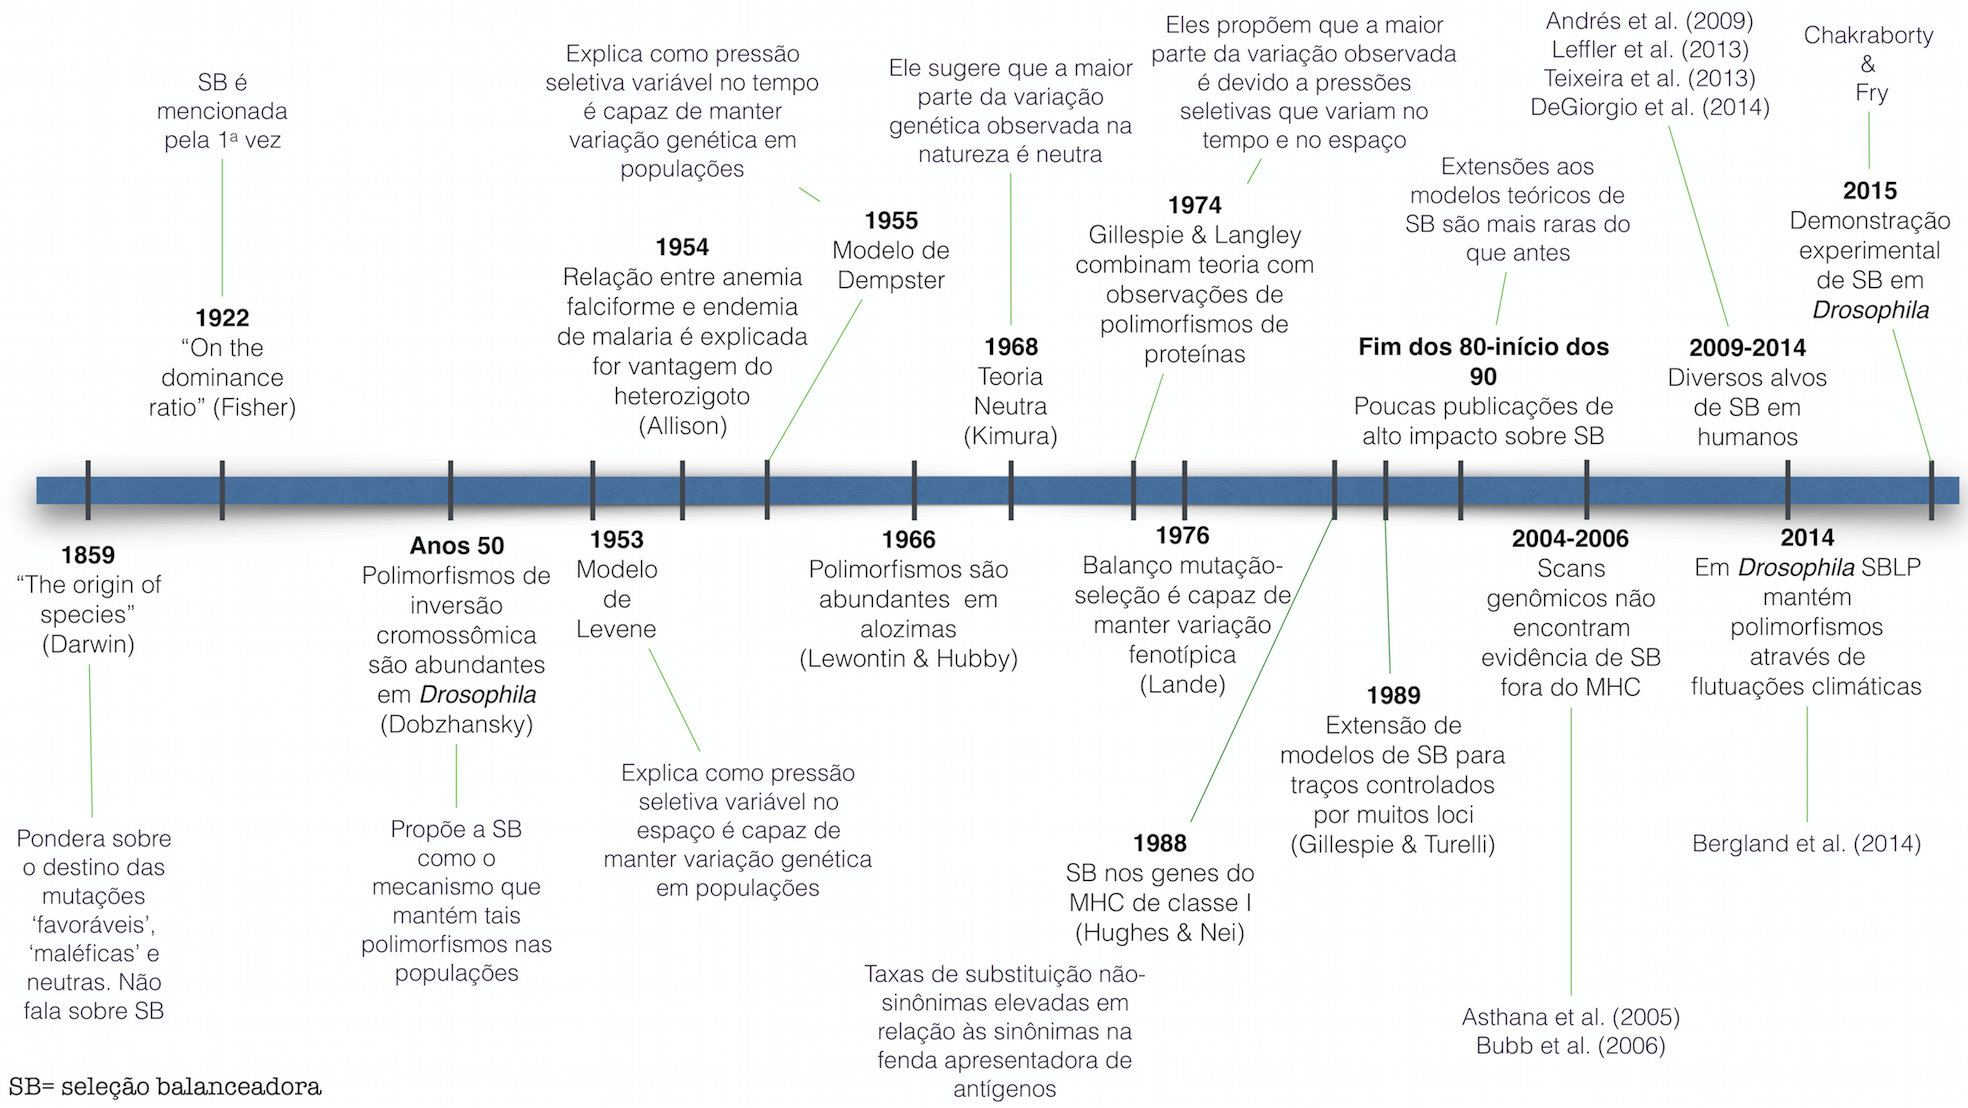
\includegraphics{chap1_folder/Figures/Figura_linha_do_tempo_v2.png}
\caption{\textbf{Linha do tempo do estudo da seleção balancedora} Adaptada a partir de \textcite{Gloss2016} resumindo as principais contribuições teóricas e empíricas para a compreensão da importância da seleção balanceadora para a manutenção de variação genética. SBLP, seleção balanceadora de longo prazo (ver texto).} %melhorar legenda pra essa fig.
\label{fig:LinhadoTempo}
\end{sidewaysfigure} 
%%%%%%%%%%%%%%%%%%%%%%%%%%%%%%%%%%%%%%%%%%%%%%%%%%%%%%%%%%%%%%%%%%%%%%%%%%%%%%%%%%%%%%%%%%%%%%%%%%%%%%%%%%%%%%%%%%
%%%%%%%%%%%%%%%%%%%%%%%%%%%%%%%%%%%%%%FIGURE FIGURE FIGURE%%%%%%%%%%%%%%%%%%%%%%%%%%%%%%%%%%%%%%%%%%%%%%%%%%%%%%%%
%%%%%%%%%%%%%%%%%%%%%%%%%%%%%%%%%%%%%%%%%%%%%%%%%%%%%%%%%%%%%%%%%%%%%%%%%%%%%%%%%%%%%%%%%%%%%%%%%%%%%%%%%%%%%%%%%%
%



%%%%%%%%%%%%%%%%%%%%%%%%%%%%%%%%%%%%%%%%%%%%%%%%%%%%%%%%%%%%%%%%%%%%%%%%%%%%%%%%%%%%%%%%%%%%%%%%%%%%%%%%%%%%%%%%%%
%%%%%%%%%%%%%%%%%%%%%%%%%%%%%%%%%%%%%FIGURE FIGURE FIGURE%%%%%%%%%%%%%%%%%%%%%%%%%%%%%%%%%%%%%%%%%%%%%%%%%%%%%%%%%
%%%%%%%%%%%%%%%%%%%%%%%%%%%%%%%%%%%%%%%%%%%%%%%%%%%%%%%%%%%%%%%%%%%%%%%%%%%%%%%%%%%%%%%%%%%%%%%%%%%%%%%%%%%%%%%%%%
\begin{figure}[h]
\centering
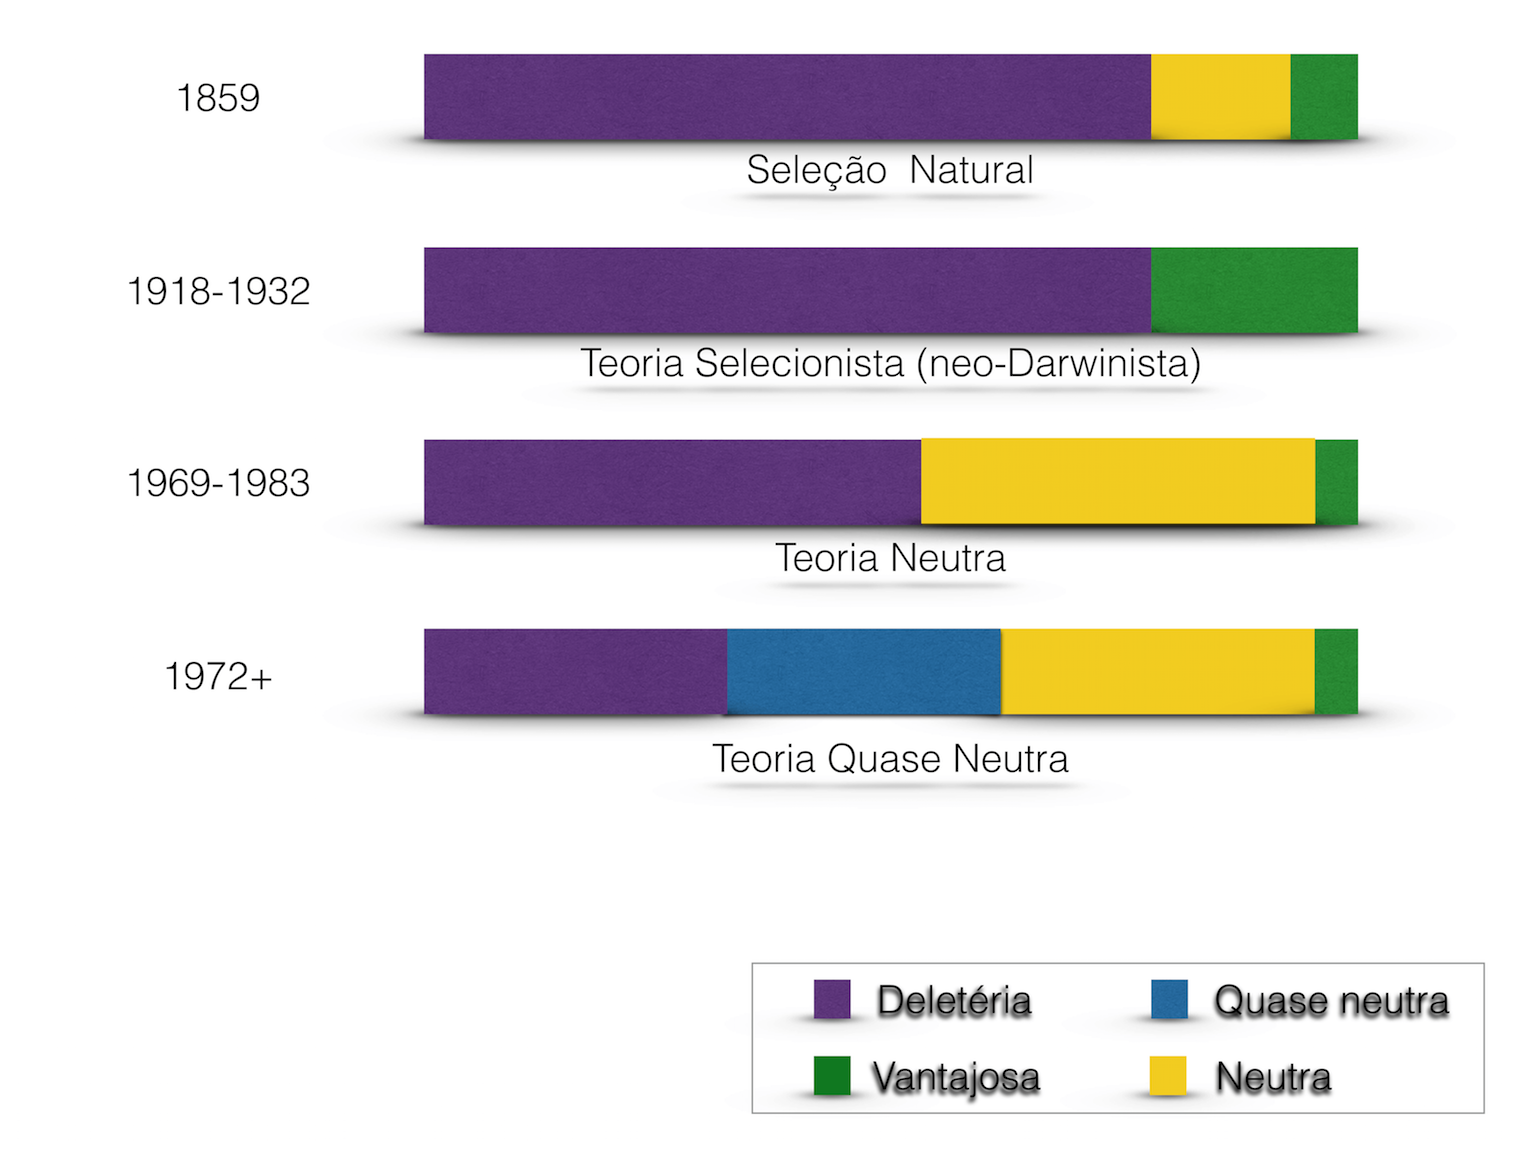
\includegraphics[height=7cm,keepaspectratio]{chap1_folder/Figures/proportion_mutations.png}
\caption{Modelos selecionista, neutro e quase neutro de evolução molecular. Figura adaptada a partir de \textcite{Bromham2003,Bernardi2007}. Em 1859, Darwin publica o livro "A origem das espécies", no qual descreve suas ideias sobre seleção natural\nocite{Darwin1979}. Darwin acredita que possam haver mutações neutras,  porém a maioria das mutações são deletérias e poucas são vantajosas. Na primeira metade do século 20 a seleção natural é conciliada com as bases do mecanismo molecular de herança (Neo-Darwinismo). Neste período, o foco selecionista aborda apenas mutações deletérias e vantajosas. Em 1968 Kimura publica a primeira versão do modelo neutro de evolução molecular (e uma atualização importante em 1983) e em 1973 Ohta \nocite{Ohta1973SlightlyEvolution} propõe o modelo quase neutro de evolução molecular. Esses dois últimos autores mostram que a deriva genética pode manter variantes neutras ou quase neutras nas populações. Ver também Figura ~\ref{fig:LinhadoTempo}.} 
\label{fig:ProportionMutations}
\end{figure}
%%%%%%%%%%%%%%%%%%%%%%%%%%%%%%%%%%%%%%%%%%%%%%%%%%%%%%%%%%%%%%%%%%%%%%%%%%%%%%%%%%%%%%%%%%%%%%%%%%%%%%%%%%%%%%%%%%
%%%%%%%%%%%%%%%%%%%%%%%%%%%%%%%%%%%%%FIGURE FIGURE FIGURE%%%%%%%%%%%%%%%%%%%%%%%%%%%%%%%%%%%%%%%%%%%%%%%%%%%%%%%%%
%%%%%%%%%%%%%%%%%%%%%%%%%%%%%%%%%%%%%%%%%%%%%%%%%%%%%%%%%%%%%%%%%%%%%%%%%%%%%%%%%%%%%%%%%%%%%%%%%%%%%%%%%%%%%%%%%%
%%%%%%%%%%%%%%%%%%%%%%%%%%%%%%%%%%%%%%%%%%%%%%%%%%%%%%%%%%%%%%%%%%%%%%%%%%%%%%%%%%%%%%%%%%%%%%%%%%%%%%
\subsection{Outra}%%%%%%%%%%%%%%%%%%%%%%%%%%%%%%%%%%%%%%%%%%%%%%%%%%%%%%
%%%%%%%%%%%%%%%%%%%%%%%%%%%%%%%%%%%%%%%%%%%%%%%%%%%%%%%%%%%%%%%%%%%%%%%%%%%%%%%%%%%%%%%%%%%%%%%%%%%%%%%%%%%%%%%%%%%%%%%%%%%%%%%%%%%%%%%%%%%%%%%%%%%%%%%%%%%%%%%%%%%%%%%%%%%%%%%%%%%%%%%%%%%%%%%%%%%%%%%%%%%%%%%%%%%%%%%%%%%%%%%%%%%%%%%%%%%%%%%%%%%%%%%%%%%%%%%%%%%%%%%%%%%%%%%%%%
\subsection{Mecanismos de manutenção de diversidade adaptativa}%%%%%%%%%%%%%%%%%%%%%%%%%%%%%%%%%%%%%%%%%%%%%%%%%%%%%%%%%%%%%%%%%%%%%%%%%%%%%%%%%
%%%%%%%%%%%%%%%%%%%%%%%%%%%%%%%%%%%%%%%%%%%%%%%%%%%%%%%%%%%%%%%%%%%%%%%%%%%%%%%%%%%%%%%%%%%%%%%%%%%%%%
%%%%%%%%%%%%%%%%%%%%%%%%%%%%%%%%%%%%%%%%%%%%% SEGUNDA PARTE DA INTRODUÇÃO %%%%%%%%%%%%%%%%%%%%%%%%%%%%%%%%%%%%%%%%
%%%%%%%%%%%%%%%%%%%%%%%%%%%%%%%%%%%%%%%%%%%%%%%%%%%%%%%%%%%%%%%%%%%%%%%%%%%%%%%%%%%%%%%%%%%%%%%%%%%%%%%%%%%%%%%%%%%%%%%%%%%%%%%%%%%%%%%%%%%%%%%%
\section{Outra seção} %%%%%%%%%%%%%%%%%%%%%%%%%%%%%%%%%%%%%%%%%%%%%%%%%%%%%%%%%%%%%%%%%%%%%%%%%%%%%%%%%%%%%%%%%%%%%%%%%
%%%%%%%%%%%%%%%%%%%%%%%%%%%%%%%%%%%%%%%%%%%%%%%%%%%%%%%%%%%%%%%%%%%%%%%%%%%%%%%%%%%%%%%%%%%%%%%%%%%%%%%%%%%%%%%%%%%%%%%%%%%%%%%%%%%%%%%%%%%%%%%%
\medskip
\begin{quotation}
\enquote{\emph{Algo bonito e relevant}}   (\cite{})
\end{quotation}
\medskip
%%%%%%%%%%%%%%%%%%%%%%%
%%%%%%%%%%%%%%%%%%%%%%%
Conteúdo.
%%%%%%%%%%%%%%%%%%%%%%%%%%%%%%%%%%%%%%%%%%%%%%%%%%%%%%%%%%%%%%%%%%%%%%%%%%%%%%%%%%%%%%%%%%%%%%%%%%%%%%%%%%%%%%%%%%%%%%%%%%%%%%%%%%%%%%%%%%%%%%%%
%%%%%%%%%%%%%%%%%%%%%%%%%%%%%%%%%%%%%%%%%%%%%%%%%%%%%%%%%%%%%%%%%%%%%%%%%%%%%%%%%%%%%%%%%%%%%%%%%%%%%%%%%%%%%%%%%%%%%%%%%%%%%%%%%%%%%%%%%%%%%%%%
%importante: tudo que for levantado aqui tem que ser respondido nos caps 1 e 2 e recapitulado nas conclusões.
%%%%%%%%%%%%%%%%%%%%%%%%%%%%%%%%%%%%%%%%%%%%%%%%%
%%%%%%%%%%%%%%%%%%%%%%%%%%%%%%%%%%%%%%%%%%%%%%%%%
\newpage
\section{Relevância, Questões \& Hipóteses}%%%%%%
%%%%%%%%%%%%%%%%%%%%%%%%%%%%%%%%%%%%%%%%%%%%%%%%%
%%%%%%%%%%%%%%%%%%%%%%%%%%%%%%%%%%%%%%%%%%%%%%%%%
%
\subsection{Relevância}
Importante falar da relevância e citar referências (\cite{Nielsen2005,Sabeti2006}).

%%%%%%%%%%%%%%%%%%%%%%%%%%%%%%%%%%%%%%%%%%%%%%%%%%%%%%%%%%%%%%%%
\subsection{\label{subsec:Perguntas}Questões \& Hipóteses}
%%%%%%%%%%%%%%%%%%%%%%%%%%%%%%%%%%%%%%%%%%%%%%%%%%%%%%%%%%%%%%%%
Essa parte crucial, crianças. Caprichem.
As hipóteses exploradas nesse contexto foram: 
\begin{itemize}
\item um item
\end{itemize}

%%%%%%%%%%%%%%%%%%%%%%%%%%%%%%%%%%%%%%%%%%%%%%%%%%%%%%%%%%%%%%%%%%%%%%%%%%%%%%%%%%%%%%%%%%%%%%%%%%%%%%%%%%%%%%%%%%%%%%%%%%%%%%%%%%%%%%%%%%%%%%%%

%%Referencias para este capítulo
\renewcommand*{\bibfont}{\footnotesize}
\printbibliography[heading=bibintoc]

\end{refsection}
%%%%%%%%%%%%%%%%%%%%%%%%%%%%
%%%%%%End of INTRO %%%%%%%%%
%%%%%%%%%%%%%%%%%%%%%%%%%%%%






\begin{refsection}
\chapter{Buscando alvos de seleção balanceadora no genoma humano}
%\addcontentsline{toc}{chapter}{Capítulo 1: Uncovering targets of balancing selection in humans}
\pagestyle{fancy}
\fancyhf{}
\fancyfoot[C]{\thepage}
\rhead{Capítulo 1}
\counterwithout{equation}{chapter}
%%%%%%%%%%%%%%%%%%%%%%%%%%%%%%%%%%%%
\section{Considerações Iniciais}%%%%
%%%%%%%%%%%%%%%%%%%%%%%%%%%%%%%%%%%%
Neste capítulo apresento um manuscrito -- atualmente em revisão final pelos co-autores -- em que desenvolvemos uma nova estatística para detecção de instâncias de seleção balanceadora no genoma humano. Ela quantifica diretamente as duas principais assinaturas de regimes de seleção balanceadora atuantes por longas escalas de tempo: um excesso de alelos segregando em frequências intermediárias e um excesso de sítios polimórficos em relação às expectativas sob um modelo nulo.

Cerca de um terço dos genes que detectamos com essa nova estatística tem evidência prévia de seleção balanceadora -- de acordo com métodos e dados bastante diferentes dos nossos. Contudo, descrevemos também mais de 150 novos genes candidatos, bem como regiões não-codificadoras candidatas e as propriedades dessas regiões.

Nosso método tem maior poder que outros  descritos na literatura, e é extremamente simples de ser implementado e interpretado, além de rodar rapidamente. Combinado a um dedicado controle de qualidade dos dados utilizados, e verificação das regiões candidatas obtidas, acreditamos ter fornecido um mapa extremamente confiável da extensão das assinaturas de seleção balanceadora no genoma humano. Com este trabalho, contribuímos para a literatura (não muito extensa) de seleção balanceadora em humanos, além de propormos um método com alto poder estatístico que, em princípio, pode ser utilizado em abordagens semelhantes para outras espécies.

Este trabalho foi feito em colaboração com a pesquisadora Aida M. Andrés, do Max Planck Institute for Evolutionary Anthropology (MPI-EVA, Leipzig), que concebeu a ideia do novo método. O trabalho começou em 2013, durante meu doutorado sanduíche, e contou com a co-supervisão de Diogo Meyer e A.M.A. Contei ainda com a colaboração dos alunos Cesare de Filippo (pós-doutorando, MPI-EVA) e João C. Teixeira (doutorando, MPI-EVA). J.C.T. realizou parte das análises de enriquecimento para as regiões candidatas, e C.F. colaborou nas etapas de simulações para avaliação da estatística e na implementação do \emph{scan} em si.  

O manuscrito foi redigido por mim, juntamente A.M.A. e D.M, e todos os autores contribuíram com comentários sobre a redação do mesmo. Ele será submetido para o períódico \emph{Plos Genetics}.

Todo o material suplementar citado no texto foi disponibilizado no fim do capítulo.
%

%%%%%%%%%%%%%%%%%%%

\newpage

\begin{otherlanguage}{english}
\begin{center}
\LARGE{Uncovering targets of balancing selection in the human genome}
\end{center}

\begin{center}
Bárbara Domingues Bitarello\textsuperscript{1}, Cesare de Fillipo\textsuperscript{2}, João Teixeira\textsuperscript{2}, Diogo Meyer\textsuperscript{1}*, and Aida M. Andrés\textsuperscript{2}*
\end{center}

\small{*, co-supervised the study}
\\
\small{1, Universidade de São Paulo, São Paulo, Brazil}
\\
\small{2,Max Planck Institute for Evolutionary Anthropology, Leipzig, Germany}

\section{Introduction}

%%%%%%%%%%%%%%%%%%%%%%%%%%%%%%%%%%%%%%%%%%%%%%%%%%%%%%%%%%%%%%%%%%%%%%%%%%%%%%%%%%%%%%%%%%%%%%%%%%%%%%%%%%%%%%%%%%%%%%%%%
%%%%%%%%%%%%%%%%%%%%%%%%%%%%%%%%%%%%%%%%%%%%%%%%%%%%%%%%%%%%%%%%%%%%%%%%%%%%%%%%%%%%%%%%%%%%%%%%%%%%%%%%%%%%%%%%%%%%%%%%%%%%%%%%%%%%%%%%%%%%%%%%
%%%%%%%%%%%%%%%%%%%%%%%%%%%%%%%%%%%%%%%%%%%%%%%%%%%%%%%%%%%%%%%%%%%%%%%%%%%%%%%%%%%%%%%%%%%%%%%%%%%%%%%%%%%%%%%%%%%%%%%%%%%%%%%%%%%%%%%%%%%%%%%%
\lettrine[lines=3]{\color{airforceblue}B}{alancing selection} refers to a class of selective mechanisms that maintain advantageous genetic diversity in populations. Although perhaps not a pervasive form of natural selection, balancing selection maintains genetic diversity with phenotypic relevance. For example, decades of research have established HLA genes as a prime example of balancing selection \parencite{Meyer2001a,Spurgin2010} with thousands of alleles segregating in humans, extensive support for the functional relevance of polymorphism (e.g., \cite{Hedrick1991,Prugnolle2005}) and various well-documented cases of association between selected alleles and disease resistance and susceptibility (e.g. \cite{Raychaudhuri2012,Howell2014}).

The catalog of well-understood non-HLA targets of balancing selection remains small, but genes identified are associated to phenotypes such as auto-immune diseases (\cite{Raychaudhuri2012}), malaria resistance (\cite{MalariaGenomicEpidemiologyNetwork2015}), resistance to HIV infection (\cite{Biasin2007}) and polycystic ovary syndrome (\cite{Day2015}). Thus, the relevance of balanced polymorphisms is not restricted to their historical influence on individual fitness: they also shape, today, human phenotypic diversity and susceptibility to disease.

Balancing selection encompasses several mechanisms (\cite{Andres2011,Charlesworth2010,Clarke1962,Fijarczyk2015}; reviewed in \cite{Andres2011,Key2014b}). These include heterozygote advantage (or overdominance) (\cite{Andres2011,Key2014b,Fijarczyk2015}), frequency-dependent selection, including rare allele advantage (\cite{Clarke1962,Charlesworth2010}), selective pressures that fluctuate in time (\cite{Andres2011,Bergland2014,Fijarczyk2015}) or in space in panmitic populations (\cite{Andres2011,Charlesworth1997,Charlesworth2006,Fijarczyk2015,Key2014b}) and cases of pleiotropy (\cite{Johnston2013}). For some mechanisms, including overdominance, pleiotropy, and some instances of selection that varies in space, a stable equilibrium can be reached (\cite{Charlesworth2010}). For other mechanisms the frequency of the selected allele can change in time with no theoretical equilibrium frequency, although the frequency of the balanced polymorphism will be strongly affected by the selective process. 

Regardless of the mechanism, balancing selection can increase genetic variation with respect to neutral expectations and has the potential to leave identifiable signatures in genomic data. These include local site-frequency spectra with an excess of alleles close to the frequency of the balanced allele and, when selection is old enough, an excess of polymorphisms relative to divergence (reviewed in \cite{Key2014b}). In some cases, very ancient balancing selection can maintain trans-species polymorphisms in sister species (\cite{Leffler2013a,Teixeira2015}), while recent balancing selection or selection that is transient (e.g., that predicted in the model of \cite{Sellis2011a}) will result in signatures that are probably difficult to distinguish from incomplete, recent positive selection sweeps (\cite{Key2014b}).


While balancing selection has been extensively explored from a theoretical perspective, an empirical understanding of its prevalence in the human genome lags behind our knowledge of positive selection. This stems from technical difficulties in detecting balancing selection, as well as the perception that balancing selection may be rare (\cite{Hedrick2012}). In fact, few methods have been developed to identify its targets, and only a handful of studies have sought to uncover targets of balancing selection genome-wide (\cite{Andres2009,Alonso2008,Kummerfeld2005,Bubb2006,Leffler2013a,DeGiorgio2014,Rasmussen2014,Teixeira2015}), with different methods and datasets. \textcite{Andres2009} and \textcite{DeGiorgio2014} identified, with different approaches, genes (\cite{Andres2009}) or genomic regions (\cite{DeGiorgio2014}) with an excess of polymorphism and with site-frequency spectra showing an excess of intermediate frequency alleles.


\textcite{Leffler2013a} and \textcite{Teixeira2015} identified trans-species polymorphisms between humans and other primates. Overall, these studies suggested that balancing selection may act on a relatively small portion of the genome, although the limited extent of the data available (e.g. exome data in \cite{Andres2009} and small sample size in \cite{DeGiorgio2014}), and the stringency of the criteria - e.g., balanced polymorphisms that pre-date human-chimpanzee divergence in \textcite{Leffler2013a, Teixeira2015} - may underlie the paucity of targets detected. 


Here, we developed two new test statistics that summarize, directly and in a simple way, the degree to which allele frequencies in a genomic region deviate from the frequencies expected under balancing selection. Through extensive simulations, we showed that one of our methods outperforms existing methods for realistic demographic scenarios for human populations. We applied our statistic to the genome-wide 1000 Genomes Project (\cite{Abecasis2012}) data in four human populations and used both outlier and simulation-based cut-offs to identify both known and new genomic regions that have evolved under long-term balancing selection.

%%%%%%%%%%%%%%%%%%%%%%%%%%%%%%%%%%%%%%%%%%END OF INTRO%%%%%%%%%%%
\section{Results}
\subsection{NCD Method}
\paragraph{Background} Owing to linkage, the signature of long term balancing selection (LTBS) on a site extends to the genetic neighborhood of the selected variant(s), so the patterns of polymorphism and divergence in a genomic region can be used to infer whether it evolved under balancing selection \parencite{Charlesworth2006,Andres2011}. LTBS leaves two distinctive signatures in linked variation, when compared with neutral expectations. The first is an increase in the ratio of polymorphic to divergent sites. This occurs because, by reducing the probability of fixation, balancing selection increases the local TMRCA \parencite{Hudson1988}. One commonly used test to detect this signature is the HKA test \parencite{Hudson1987}.

The second signature is an excess of alleles segregating at intermediate frequencies. In humans, the folded  site frequency spectrum (SFS), which is the distribution of the frequency of the minor alleles (MAF) regardless of whether they are ancestral or derived, is typically L-shaped, showing an excess of low-frequency alleles when compared to expectations under neutrality and demographic equilibrium. This is a consequence of recent population expansions (e.g. \cite{Coventry2010}), with the abundance of rare alleles further increased by purifying selection and recent selective sweeps. On the other hand, regions under LTBS are expected to show a markedly different SFS, with proportionally more alleles at intermediate frequency (Fig 1A-B). Such a deviation in the SFS is the signature identified by classical neutrality tests, such as Tajima’s D (\cite{tajima1989statistical}) and newer statistics such as MWU-high (\cite{Nielsen2009}).

%%%%%%%%%%%%%%%%%%%%%%%%%%%%%%%%%%%%%%%%%%%%%%%%%%%%%%%%%%%%%%%%%%%%%%%%%%%%%%%%%%%%%%%%%%%%%%%%%%%%%%%%%%%%%%%%%%%%%%%%
%%%%  Figure 1  %%%%%%
%%%%%%%%%%%%%%%%%%%%%%
\begin{figure}
\includegraphics[]{chap2_folder/Figures/Fig1.tiff}
\caption*{\textbf{Figure 1. Schema for NCD statistics definition}\\ 
\textbf{(A)} Schematic representation of distributions of derived allele frequencies (unfolded SFS) expected for loci under neutrality (grey), containing one site under balancing selection with frequency equilibrium of 0.5 (blue), 0.4 (orange) and 0.3 (pink). DAF is the derived allele frequency, ranging from 0 to 1. \textbf{(B)} Schematic representations of distributions of minor allele frequencies (folded SFS), ranging from 0 to 0.5. Colors as in \textbf{A}. \textbf{(C)} Schematic representation of density plots of the distribution of NCD expected under neutrality (grey) and under selection (following the $f_{\mathrm{eq}}$ values given in (A). 
}
\end{figure}
%%%%%%%%%%%%%%%%%%%%%%%%%%%%%%%%%%%%%%%%%%%%%%%%%%%%%%%%%%%%%%%%%%%%%%%%%%%%%%%%%%%%%%%%%%%%%%%%%%%%%%%%%%%%%%%%%%%%%%%%%%%%%%%%%%%%%%%%%%%%%%%%%%%%%%%%%%%%%%%%%%%%%%%%%%%%%%%%%%%%%%%%%%%%%%%%%%%%%%%%%%%%%%%%%%%%%%%%%%%%%%%%%%%%%%%%%%%%%%%%%%%%%%%%%%%

The signatures of LTBS on the SFS will depend on the selective regime and the intensity of selection on each genotype. For example, under overdominance the frequency equilibrium depends on the relative fitness of each genotype (\cite{Charlesworth2006,Charlesworth2010,Fijarczyk2015}). Given selection coefficients \emph{s} and \emph{t} against the AA and BB homozygotes, respectively, the deterministic frequency equilibrium ($f_{\mathrm{eq}}$) is given by:


\begin{equation}
f_{\mathrm{eq_{A}}}=\frac{s}{s+t}
\end{equation}


With symmetric overdominance ($s=t$), $f_{\mathrm{eq}}=0.5$. With asymmetric overdominance ($t \neq s$), which might be more prevalent in natural systems (\cite{Hedrick2012}), it follows that $f_{\mathrm{eq}} \neq 0.5$. A classic example of asymmetric overdominance is the case of $\beta$-globin and sickle cell anemia, where in regions of endemic malaria the fitness of the \emph{HbA} homozygote for the $\beta$-globin \label{page:HbS} locus is approximately 9 times higher than that of the \emph{HbS} homozygote, with the resulting equilibrium frequency of the \emph{HbS} allele being 0.13 (\cite{Allison1961}). Under frequency-dependent selection, $f_{\mathrm{eq}}$ will depend on the frequency of the favored allele. Under fluctuating selection the frequency of the selected allele will depend on the temporal and spatial scales of selection (\cite{Andres2011,Clarke1964,Pasvol1978}) and although no stable, long-term frequency equilibrium may be reached, the balanced polymorphism may be actively maintained (as long as the heterozygote fitness exceeds that of homozygotes in their harmonic and geometric means, for spatial and temporal models, respectively) (reviewed in \cite{Hedrick2006}). In these cases, $f_{\mathrm{eq}}$ can be thought of as the frequency, at the time of sampling, of the balanced polymorphism. 

\paragraph{Non-Central Deviation (NCD)} In the tradition of neutrality tests that analyze directly the SFS (e.g. \cite{Nielsen2005a,Nielsen2009,Williamson2007}), we propose two related test statistics that explore the abundance and frequency of polymorphisms in a given locus. Both tests measure a \enquote{Non-Central Deviation} (NCD), which we define as the degree to which the local SFS deviates from a pre-specified allele frequency (the \emph{target frequency}, $tf$). Under a model of balancing selection, $tf$ can be thought of as the deterministic frequency that would be attained given the selection parameters, with the NCD statistic querying how far SNP frequencies are from it. We propose two implementations for this statistic: $NCD1$ and $NCD2$. The $NCD1$ statistic is based solely on the SFS, using information on allelic frequency, $p_{i}$ , of each site in a locus:

\begin{equation}
NCD1_{tf}=\sqrt{\frac{\sum\limits_{i=1}^n(p_{i}-tf)^2}{n}}
\end{equation}

where $i={1,2,3,...,n}$ is the $i$-th polymorphism, $p_{i}$ is the MAF for the $i$-th polymorphism, and $tf$ is is the target frequency with respect to which the deviations of the observed alleles frequencies are computed. Thus, $NCD1$ is a non-central standard deviation that quantifies the dispersion of allelic frequencies from $tf$, rather than from the mean of the distribution. Because the frequencies of alleles at bi-allelic loci are complementary, and under balancing selection there is no prior expectation on the ancestral or the derived allele being maintained at higher frequency, we use the folded SFS (Fig 1). The minimum amount of data required for calculating $NCD1$ is one polymorphism, and for simplicity we consider only bi-allelic SNPs.

The $NCD2$ statistic is an extension of $NCD1$ that includes information not only on the frequency of polymorphisms, but also on the number of fixed differences (FDs):

\begin{equation}
NCD2_{tf}=\sqrt{\frac{n \cdot (0-tf)^2 + \sum\limits_{i=1}^n(p_{i}-tf)^2}{n_{fd}+n}}
\end{equation}

, where $n_{fd}$ is the number of FDs in the locus. In $NCD2$, all informative sites (IS = SNPs + FDs) are taken into account. FDs can be considered informative sites with a minor allele frequency (MAF) of 0, and as such they contribute to deviation from $tf$: the greater the number of fixed differences, the larger the $NCD2$ value and hence the weaker the support for LTBS. The minimal data required for calculating $NCD2$ is one informative site, and for simplicity only bi-allelic allelic SNPs and single nucleotide FDs are considered.

From equations 2 and 3 it follows that the maximum value for $NCD2_{tf}$ for a given $tf$ is the target frequency itself (i.e, no SNPs and one or more FDs in the locus, as in S1 Fig) and for $NCD1_{tf}$ the maximum value approaches - but never reaches - $tf$ when all SNPs are singletons. The minimum value for both $NCD1_{tf}$ and $NCD2_{tf}$ is 0, when all SNPs segregate at $tf$ and, in the case of $NCD2_{tf}$, there are no FDs (S2 Fig). Thus, low $NCD1$ and $NCD2$ values reflect a low deviation of the SFS from the pre-defined target frequency, which is expected in windows containing sites under LTBS (Fig 1C).
%%%%%%%%%%%%%%%%%%%%%%%%%%%%%%%%%%%%%%%%%%%%%%%%%%%%%%%%%%%%
\subsection{Power of the NCD statistics to detect LTBS}
%%%%%%%%%%%%%%%%%%%%%%%%%%%%%%%%%%%%%%%%%%%%%%%%%%%%%%%%%%%%
We evaluated the specificity and sensitivity of $NCD1$ and $NCD2$ by benchmarking their performance using simulations. Specifically, we considered demographic scenarios inferred for African, European, and Asian human populations (Fig 2), and simulated both neutrality and balancing selection using a model of heterozygote advantage (see Methods). We then explored the influence of the parameters that may affect the power of the NCD statistics: time since the onset of balancing selection (\emph{Tbs}), the deterministic frequency equilibrium defined by the selection coefficients ($f_{\mathrm{eq}}$), the demographic history of the sampled population, the chosen target frequency in NCD calculation (both for cases in which $f_{\mathrm{eq}}$ does and does not match $tf$), the length of the genomic region analyzed (\emph{L}), and the implementation of NCD ($NCD1$ or $NCD2$). Box 1 summarizes the nomenclature used throughout the text.

\fbox{\begin{minipage}{34em}
\textbf{BOX 1. List of Abbreviations}\\
LTBS, long-term balancing selection.\\
MAF, minor allele frequency.\\
SFS, site-frequency spectrum. \\
FD, fixed difference (between two species). \\
IS, informative sites (number of polymorphic sites in the ingroup species plus the number of fixed differences between ingroup and outgroup species).\\
$f_{\mathrm{eq}}$, deterministic equilibrium frequency achieved by site(s) under balancing selection as defined by the selection coefficients.\\
$tf$, target frequency, i.e, the frequency used in the NCD statistics as the value to which queried allele frequencies are compared to.\\
NCD statistics, non-central deviation statistics, with two implementations.\\
$NCD1$, NCD statistic that measures the average distance between polymorphic allele frequencies and a pre-determined frequency ($tf$). $NCD1_{tf}$ is $NCD1$ for that given $tf$. \\
$NCD2$, NCD statistic that measures the average distance between allelic frequencies and a pre-determined frequency ($tf$) considering both polymorphisms and fixed differences with an outgroup.  $NCD2_{tf}$ is $NCD2$ for that given $tf$.\\
$NCD_{tf}$ refers to the average of $NCD1_{tf}$ and $NCD2_{tf}$.\\
\end{minipage}}
\bigskip	
\bigskip


%%%%%%%%%%%%%%%%%%%%%%%%%%%%%%%%%%%%%%%%%%%%%%%%%%%%%%%%%%%%%%%%%%%%%%%%%%%%%%%%%%%%%%%%%%%%%%%%%%%%%%%%%%%%%%%%%%%%%%%%
%%%  Figure 2  %%%
%%%%%%%%%%%%%%%%%%
\begin{figure}
\begin{center}
\includegraphics[]{chap2_folder/Figures/Fig2.tiff}
\caption*{\textbf{Figure 2. Human demographic model and parameters used in simulations}\\ 
For all simulations, the human demographic model is the one inferred in Gravel et al. (2011) \nocite{Gravel2011}, including migration rates, population split times, and effective population sizes ($N_{e}$). Divergence with chimpanzees was added to this model. \emph{g}, generations; \emph{T} time in generations since different events: the split between human and chimpanzee lineages ($T_{div}$), the population growth in African ($T_{g_af}$), the out-of-Africa migration ($T_{ooa}$), and the European-Asian split ($T_{eu_as}$); \emph{N} refers to $N_{e}$ of different populations: the ancestral population ($N_{anc}$), the chimpanzee population ($N_{c}$), the ancestral human population ($N_{h}$), the African population after $T_{g_af}$ population growth ($N_{afr}$), the Eurasian ancestral population ($N_{ooa}$), the European population ($N_{eur}$) and the Asian population; \emph{r} are the growth rates of Asian and European populations. $Tbs$ is the time (in millions of years) since onset of balancing selection, and $f_{\mathrm{eq}}$ the frequency equilibrium of the balanced polymorphism.
}
\end{center}
\end{figure}
%%%%%%%%%%%%%%%%%%%%%%%%%%%%%%%%%%%%%%%%%%%%%%%%%%%%%%%%%%%%%%%%%%%%%%%%%%%%%%%%%%%%%%%%%%%%%%%%%%%%%%%%%%%%%%%%%%%%%%%%%%%%%%%%%%%%%%%%%%%%%%%%%%%%%%%%%%%%%%%%%%%%%%%

For simplicity we present power values (always at false positive rate of 5\%) averaged across NCD implementations ($NCD_{tf}$ being the average of $NCD1_{tf}$ and $NCD2_{tf}$), demographic models and sequence lengths. These averages are helpful in that they reflect the general changes in power when changing individual parameters. Nevertheless, because they often include conditions for which power is low, the averages underestimate the power that the test can reach under a given parameter. The full matrix of power results for each condition is presented in S1 Table, and some key points are discussed below.

\paragraph{Time since the onset of balancing selection and sequence length}

The signatures of LTBS are expected to be stronger the longer the time since the onset of balancing selection, because there will have been more time for linked mutations to accumulate and reach intermediate frequencies. We
simulated sequences with a balanced polymorphism with \emph{Tbs} of 1, 3, and 5 million years (myr) (Fig 2). For simplicity, in this section we consider only cases where $tf=f_{\mathrm{eq}}$ although this condition is relaxed in later sections.

For both $NCD1_{0.5}$ and $NCD2_{0.5}$ ($f_{\mathrm{eq}}=0.5$), power to detect balancing selection with $Tbs=1$ myr is low across all scenarios and for all $tf$ (always lower than 0.43, S1 Table). Nevertheless, power to identify older balanced
polymorphisms is high, for all $tf$, for both 3 myr (e.g. average $NCD_{0.5}$ is 0.70) and 5 myr (average $NCD_{0.5}$ 0.77) (S3-S8 Figs, S1 Table). We thus focus exclusively on long-term balancing selection: 3 and 5 myr.

\emph{Tbs} also affects the length of the region bearing the signature of balancing selection, as in the absence of epistasis the long-term effects of recombination result in narrower signatures with older \emph{Tbs} \parencite{Leffler2013a,Teixeira2015}. This is indeed the case for all $tf$ (S3-S8 Figs, S1 Table). For example, $NCD_{0.5}$ at $Tbs=5$ myr resulted in average power of 0.78, 0.76, and 0.67 for 3, 6, and 12 Kb, respectively (S3-S8 Figs, S1 Table), and a similar pattern emerges for $NCD_{0.4}$ and $NCD_{0.3}$. For $NCD1$ the power increment for shorter regions was less pronounced than for $NCD2$ (S1 Table), perhaps due to the lower number of informative sites. Again, a similar picture emerges for $NCD_{0.4}$ – with 21\% reduction in power for 12 Kb compared to 3 Kb – and $NCD_{0.3}$ – with 25\% reduction in power for 12 Kb compared to 3 Kb (S1 Table; S3-S8 Figs).

In summary, the power of the NCD statistics grows with the age of the balanced polymorphism and the narrowness of the analyzed window. These analyses suggest that the NCD statistics are well powered to detect balancing selection that started at least 3 myr ago in windows of 3 Kb centered on the selected site (S1 Table) and we therefore do not include 1 myr results in the remainder of the discussion.

\paragraph{Demography} Power is similar for samples simulated under the African (average $NCD_{0.5}$ of 0.86) and European (average $NCD_{0.5}$ of 0.87) demographic scenarios for both $NCD1_{0.5}$ and $NCD2_{0.5}$ and drastically lower for a population under the demographic model for Asians (average $NCD_{0.5}$ of 0.48; S3-S8 Figs, and S1 Table). Similar trends are observed for $NCD_{0.4}$ (75\% average reduction in Asia when compared with Africa) and $NCD_{0.3}$ (92\% reduction). One explanation for the lower power under the Asian demographic model is the stronger effect of random genetic drift in this population due to its lower $N_{e}$ (\cite{Gutenkunst2009,Gravel2011}), which affects both the SFS of neutral loci (putatively increasing the proportion of alleles at intermediate frequency) and those under balancing selection (reducing the efficacy of selection and putatively increasing the dispersion from the balanced frequency equilibrium). We thus focused our subsequent analyses on the African and European populations, for which power was high and comparable (thus allowing fair comparisons between these geographic regions).

\paragraph{Simulated and target frequencies} So far we discussed only cases where $tf=f_{\mathrm{eq}}$, which is expected to favor the performance of the method. In this case the NCD statistics have high power: on average 0.86, 0.79, and 0.70 for $f_{\mathrm{eq}}=$ 0.5, 0.4, and 0.3, respectively (S1 Table). Selection with $f_{\mathrm{eq}}$=0.2 resulted in low power across all parameters and $tf$ values (S3-S8 Figs), so we do not further explore this target frequency. 

In practice, though, one does not have \emph{a priori} knowledge about the equilibrium frequency of balanced polymorphisms. We thus explored the power of NCD when the simulated equilibrium and the target frequencies differ. The power to detect LTBS is very high for $NCD2_{0.5}$ and $NCD1_{0.5}$, even when selection is simulated with other $f_{\mathrm{eq}}$ values (average $NCD_{0.5}$  of 0.79, Table 1, S3-S8 Figs, and S1 Table) and similarly high for $NCD_{0.4}$ (average 0.78) and $NCD_{0.3}$ (average 0.70) (S1 Table). 

Conversely, power to detect LTBS with $f_{\mathrm{eq}}=0.4$ is similar with $NCD_{0.5}$ or $NCD_{0.4}$ (Table 1 and S1 Table), but for $f_{\mathrm{eq}}=0.3$ power is 10\% is higher for $NCD_{0.3}$ than for $NCD_{0.5}$ (Table 1 and S1 Table). Therefore, NCD statistics can be well powered both when the frequency of the balanced polymorphism is the same as the target frequency, and when it is not (as expected given correlations among these statistics; S9 Fig). Nevertheless, the closest $tf$ is to $f_{\mathrm{eq}}$, the highest the power to identify targets of LTBS (Table 1). Thus, information is gained by calculating NCD with different target frequencies. 

%%%%%%%%%%%%%%%%%%%%%%%%%%%%%%%%%%%%%%%%%%%%%%%%%%%%%%%%%%%%%%%
% Please add the following required packages to your document preamble:
% \usepackage{booktabs}
% \usepackage[table,xcdraw]{xcolor}

% If you use beamer only pass "xcolor=table" option, i.e. \documentclass[xcolor=table]{beamer}

%%%%%%%%%%%%%%%%%%%%%%%%%%%%%%%%
%%%%%%%%%%%%%%%%%%%%%%%%%%%%%%%%
%%%%%%%%%%%%%%%%%%%%%%%%%%%%%%%%
\begin{table}[]
\centering
\caption*{\textbf{Table 1. Power for simulations under the African and European demographic models}\\
\emph{Tbs}, time since onset of balancing selection (in millions of years); $f_{\mathrm{eq}}$, frequency equilibrium in the simulations. Power values are for a false positive rate of 0.05, for simulations of the African and European demographic scenarios, $L=3$ Kb.}
\label{table1manuscript}
\resizebox{\textwidth}{!}{%
\begin{tabular}{llllllllllllll}
 &  & \multicolumn{6}{c}{\cellcolor[HTML]{C0C0C0}Africa} & \multicolumn{6}{c}{\cellcolor[HTML]{C0C0C0}Europe} \\
 &  & \multicolumn{3}{c}{\cellcolor[HTML]{EFEFEF}$NCD2$} & \multicolumn{3}{c}{\cellcolor[HTML]{EFEFEF}$NCD1$} & \multicolumn{3}{c}{\cellcolor[HTML]{EFEFEF}$NCD2$} & \multicolumn{3}{c}{\cellcolor[HTML]{EFEFEF}$NCD1$}\\
 &  & \multicolumn{3}{c}{\cellcolor[HTML]{EFEFEF}$tf$} & \multicolumn{3}{c}{\cellcolor[HTML]{EFEFEF}$tf$} & \multicolumn{3}{c}{\cellcolor[HTML]{EFEFEF}$tf$} & \multicolumn{3}{c}{\cellcolor[HTML]{EFEFEF}$tf$} \\
\rowcolor[HTML]{C0C0C0} 
\cellcolor[HTML]{EFEFEF}\emph{Tbs} & $f_{\mathrm{eq}}$ & 0.5 & 0.4 & 0.3 & 0.5 & 0.4 & 0.3 & 0.5 & 0.4 & 0.3 & 0.5 & 0.4 & 0.3 \\
\cellcolor[HTML]{EFEFEF}5 & \cellcolor[HTML]{C0C0C0}0.5 & 0.96 & 0.94 & 0.84 & 0.93 & 0.91 & 0.39 & 0.97 & 0.95 & 0.83 & 0.92 & 0.85 & 0.20 \\
\cellcolor[HTML]{EFEFEF}5 & \cellcolor[HTML]{C0C0C0}0.4 & 0.94 & 0.94 & 0.89 & 0.89 & 0.89 & 0.67 & 0.95 & 0.94 & 0.91 & 0.85 & 0.82 & 0.59 \\
\cellcolor[HTML]{EFEFEF}5 & \cellcolor[HTML]{C0C0C0}0.3 & 0.90 & 0.91 & 0.93 & 0.72 & 0.80 & 0.84 & 0.84 & 0.85 & 0.89 & 0.47 & 0.57 & 0.74 \\
\cellcolor[HTML]{EFEFEF}3 & \cellcolor[HTML]{C0C0C0}0.5 & 0.91 & 0.88 & 0.68 & 0.86 & 0.80 & 0.24 & 0.93 & 0.89 & 0.68 & 0.81 & 0.69 & 0.14 \\
\cellcolor[HTML]{EFEFEF}3 & \cellcolor[HTML]{C0C0C0}0.4 & 0.88 & 0.86 & 0.76 & 0.78 & 0.78 & 0.56 & 0.89 & 0.87 & 0.79 & 0.74 & 0.71 & 0.46 \\
\cellcolor[HTML]{EFEFEF}3 & \cellcolor[HTML]{C0C0C0}0.3 & 0.75 & 0.77 & 0.81 & 0.56 & 0.64 & 0.71 & 0.73 & 0.76 & 0.79 & 0.39 & 0.48 & 0.63 \\ \hline
\end{tabular}%
}
\end{table}
%%%%%%%%%%%%%%%%%%%%%%%%%%%%%%%%%%%%%%%%%%%%%%%%%%%%%%%%%%%%%%%%%%%%%%%%%%%%%%%%%%%%%%%%%%%%%%%%%%%%%%%%%%%%%%%%%%%%%%%%%%%%%%%%%%%%%%%%%%%%%%%%
%%%%TABLE %%% TABLE %%% TABLE %%%% TABLE %%%%%%%TABLE %%% TABLE %%% TABLE %%%% TABLE %%%%%%%TABLE %%% TABLE %%% TABLE %%%% TABLE %%%%%%%TABLE %%
%%%%%%%%%%%%%%%%%%%%%%%%%%%%%%%%%%%%%%%%%%%%%%%%%%%%%%%%%%%%%%%%%%%%%%%%%%%%%%%%%%%%%%%%%%%%%%%%%%%%%%%%%%%%%%%%%%%%%%%%%%%%%%%%%%%%%%%%%%%%%%%%

\paragraph{NCD implementations}
The power for $NCD2$ is greater than for $NCD1$, for all $tf$: $f_{\mathrm{eq}}=0.5$ (average power of 0.94 for $NCD2_{0.5}$ and 0.88 for $NCD1_{0.5}$), $f_{\mathrm{eq}}=0.4$ (0.93 for $NCD2_{0.4}$ and 0.80 for $NCD1_{0.4}$) and for $f_{\mathrm{eq}}=0.3$ (0.85 for $NCD2_{0.3}$ and 0.73 for $NCD1_{0.3}$ (Table 1, Fig 3, S1 Table). The gain in power that occurs when using information on FDs was also explored by jointly considering $NCD1$ with HKA (see below). 


%%%%%%%%%%%%%%%%%%%%%%%%%%%%%%%%%%%%%%%%%%%%%%%%%%%%%%%%%%%%%%%%%%%%%%%%%%%%%%%%%%%%%%%%%%%%%%%%%%%%%%%%%%%%%%%%%%%%%%%%%%%  Figure 3 %%%
%%%%%%%%%%%%%%%%%
\begin{sidewaysfigure}
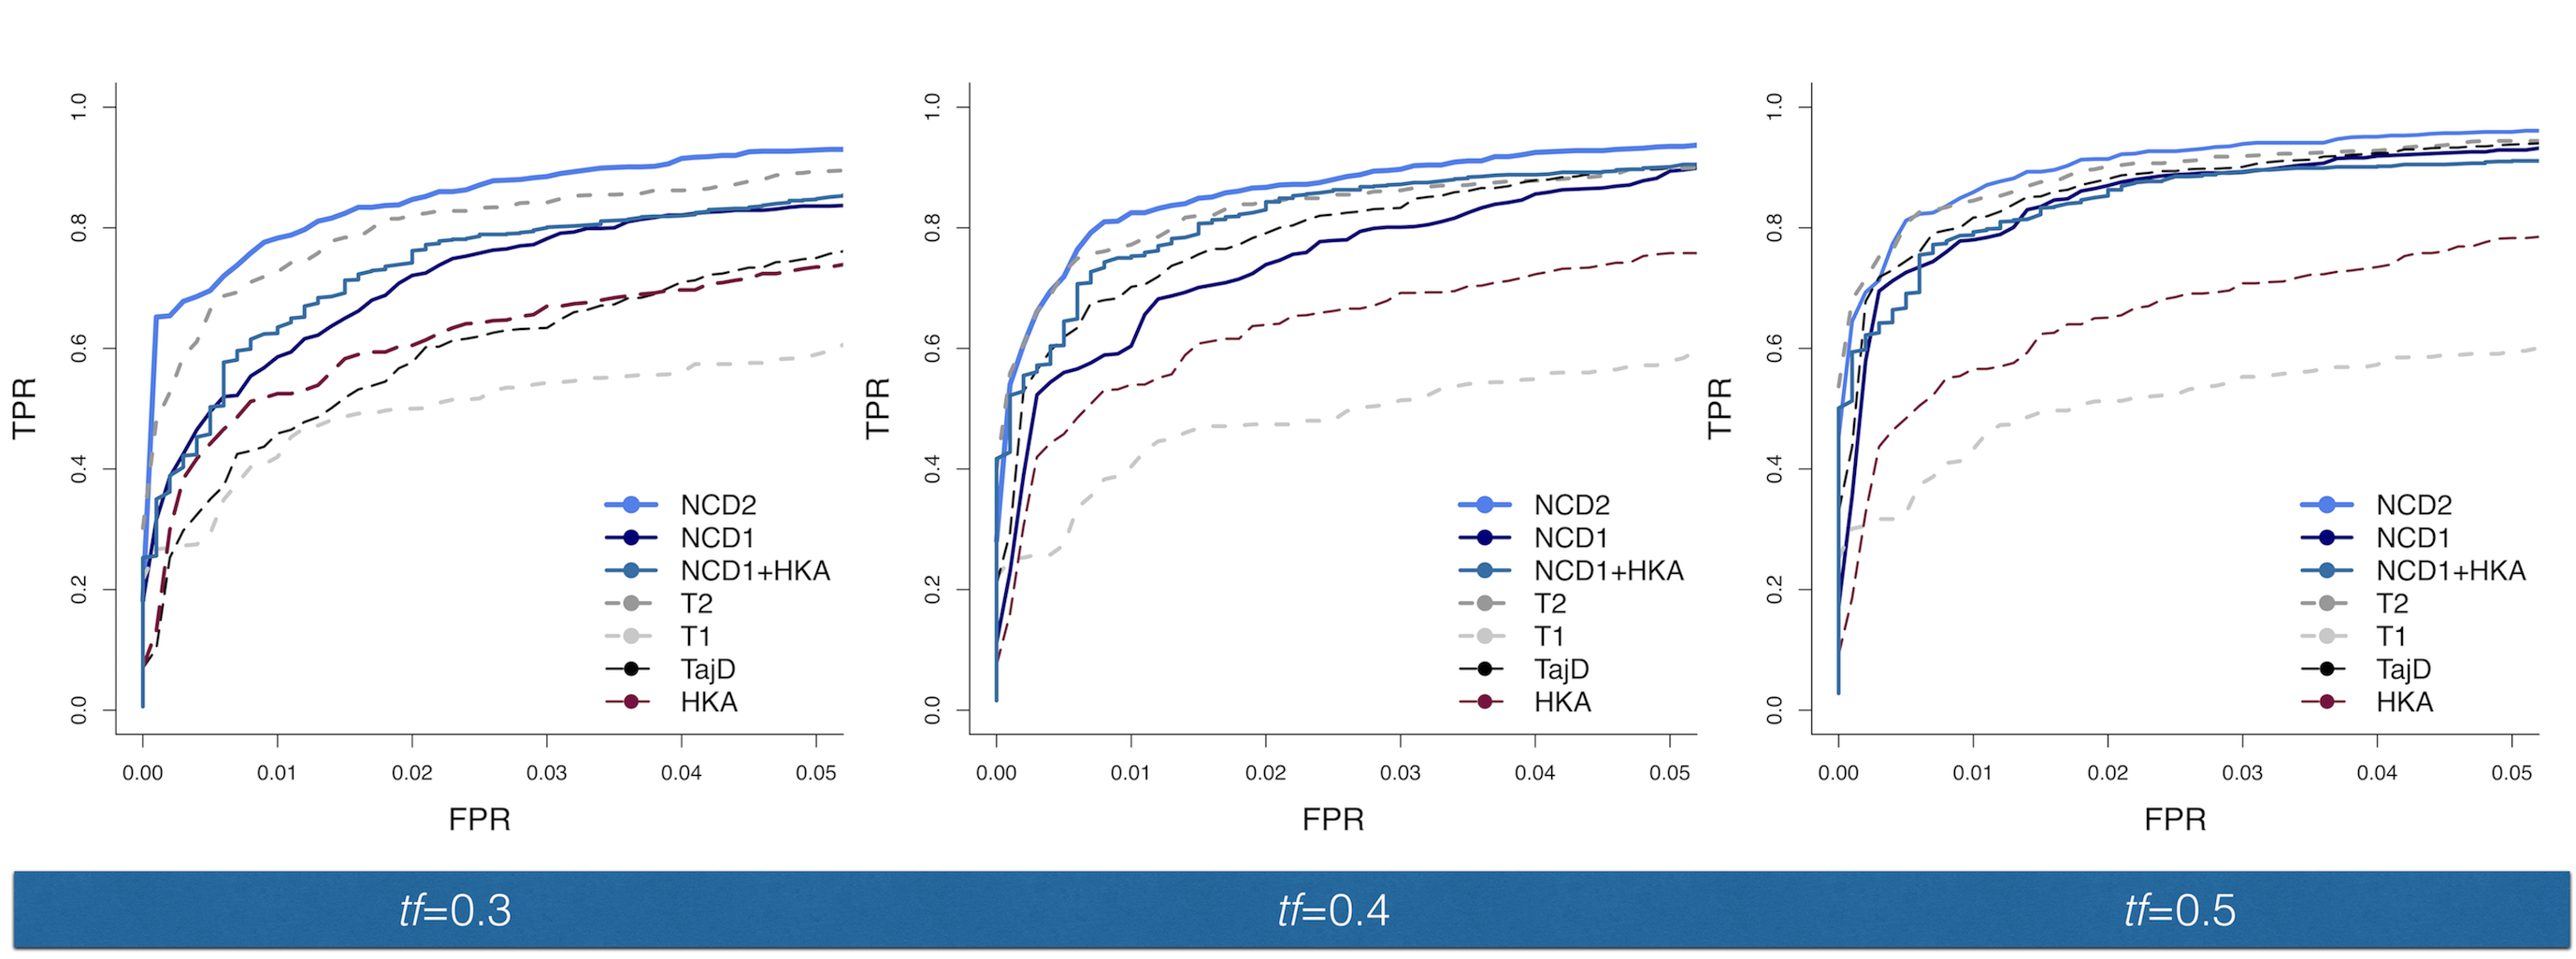
\includegraphics[]{chap2_folder/Figures/Fig3.png}
\caption*{\textbf{Figure 3. ROC curves for comparison between $NCD2_{0.5}$ and other tests}\\
Power to detect LTBS for simulations where the balanced polymorphism was modeled to achieve frequency equilibrium ($f_{\mathrm{eq}}$) of \textbf{A)} 0.3, \textbf{B)} 0.4, and \textbf{C)} 0.5. Plotted values are for African demography, $Tbs = 5$ myr, $L = 3$ kb, except for T1 and T2 \parencite{DeGiorgio2014}, which were evaluated based on 100 SNPs in 15 Kb simulated windows following the original publication (see Methods). Target frequency for $NCD1$ and $NCD2$ matches the simulated $f_{\mathrm{eq}}$. Similar results are observed for European demography (Fig S7).}
\end{sidewaysfigure}
%%%%%%%%%%%%%%%%%%%%%%%%%%%%%%%%%%%%%%%%%%%%%%%%%%%%%%%%%%%%%%%%%%%%%%%%%%%%%%%%%%%%%%%%%%%%%%%%%%%%%%%%%%%%%%%%%%%%%%%%%%%%%%%%%%%%%%%%%%%%%%%%%%%%%%%%%%%%%%%%%%%%%%%%%%%%%%%%%%%%%%%%%%%%%%%%%%%%%%%%%%%%%%%%%%%%%%%%%%%%%%%%%%%%%%%%%%%%%%%%%%%%%%%%%%%


\paragraph{NCD statistics compared to existing methods} We compared the power of $NCD2_{0.5}$ to other statistics commonly used to detect balancing selection. We focused on Tajima’s \emph{D} (Taj\emph{D}) and HKA (\cite{Hudson1987,tajima1989statistical}), a pair of composite likelihood-based measures recently developed by \textcite{DeGiorgio2014} termed T1 and T2 (T1 only looks at the SFS, T2 includes information on FDs), and $NCD1$ and $NCD2$. We additionally explored the power of a composite statistic, where the \emph{p}-value was jointly computed as a function of $NCD1$ and HKA statistics ($NCD1$+HKA), with the goal of quantifying the contribution of FDs to NCD power (see Methods). For simplicity we considered $Tbs=5$ my and 3 Kb for all comparisons. The only exceptions are T1 and T2, for which a larger window size (100 informative sites) was used, following \textcite{DeGiorgio2014}, to compare the methods using their optimal window size. 

When $f_{\mathrm{eq}}=0.5$, $NCD2_{\mathrm{0.5}}$ has the highest power: 0.96 (0.94 for T2, 0.93 for Taj\emph{D}, 0.91 for $NCD1_{0.5}$+HKA, 0.78 for HKA, and 0.5 for T1; Fig 3). The gain in power provided by $NCD2_{0.5}$ is much higher when $f_{\mathrm{eq}}$ departs from 0.5, where $NCD2$ clearly outperforms all other tests if $tf=f_{\mathrm{eq}}$ (Fig 3). For $f_{\mathrm{eq}}=0.4$, the power of $NCD2_{0.4}$ is 0.94 (0.9 for Taj\emph{D}, T2, and $NCD1_{0.5}$+HKA; 0.76 for HKA, and 0.58 for T1; Fig 3 and Table 1) and for $f_{\mathrm{eq}}=0.3$ $NCD2_{0.3}$ power is 0.91 (0.89 for T2, 0.85 for $NCD1_{0.5}$+HKA, 0.75 for Taj\emph{D}, 0.73 for HKA, 0.59 for T1; Fig 3). These patterns are consistent in both African and European simulations (Fig 3, Table 1, S10 Fig). Thus, $NCD2$ has greater or comparable power to detect LTBS than Taj\emph{D}, HKA, T1 and T2, and a combined test of $NCD1$+HKA for African and European scenarios (Fig 3, Table 1, S7 Fig). Notably, as the simulated frequency equilibrium moves away from 0.5, its advantage over Taj\emph{D} increases (Fig 3).

\paragraph{Recommendations based on power analyses.} Overall, $NCD1$ and $NCD2$ perform very well in regions of 3 Kb (Table 1, Fig 3). In fact, $NCD2$ outperforms all other methods tested (Table1 , Fig 3) and it reaches very high power when $tf=f_{\mathrm{eq}}$ (higher than 0.9 for 5 myr alleles and than 0.79 for 3 myr alleles). While the $f_{\mathrm{eq}}$ of a putatively balanced allele is unknown, the simplicity of the statistic makes it trivial to run it for several $tf$ values. Importantly, power was very similar under the African and European models (Table 1, Fig 3, S10 Fig). Because $NCD2$ outperforms $NCD1$ we recommend using of $NCD2$ in humans, although $NCD1$ is a good choice when outgroup data is lacking.



%%%%%%%%%%%%%%%%%%%%%%%%%%%%%%%%%%%%%%%%%%%%%%%%%%%%%%
%i stopped here 26.5

\subsection{Identifying signatures of LTBS in the human genome}

We aimed to identify regions of the genome under LTBS. Based on the power analyses, we used $NCD2_{0.5}$, $NCD2_{0.4}$ and $NCD2_{0.3}$, which are well powered to detect LTBS and do not provide fully overlapping sets of candidate windows. We calculated these statistics for 3kb windows (1.5kb step size) and tested for significance using two complementary approaches: one based on neutral expectations, and one based on the empirical data. We analyzed genome-wide data from two of African (YRI: Yoruba in Ibadan, Nigeria; LWK: Luhya in Webuye, Kenya) and two European populations (GBR: British from England and Scotland; TSI:Toscani in Italy) (\cite{Abecasis2012}). We filtered for mappability, segmental duplications, and orthology with the outgroup genome (chimpanzee, see Methods and S13 Fig).

In addition, because windows with a low number of IS have high $NCD2$ variance due to noisy SFS (S18 Fig), a pattern also observed in neutral simulations (S11 Fig), we excluded windows with less than 19 and 15 IS in African and European populations, respectively. This filter removed only 4\% of the windows while keeping a set of windows for which $NCD2$ values remain quite stable regardless of the number of IS (S11-S18 Figs). After all filters, the genomic coordinates defining the windows were identical in all populations, allowing comparisons among them. We analyzed 1,631,372 windows throughout the genome (Table 2, S13 Fig). These windows overlapped 18,308 protein-coding genes (95\% of all human autosomal genes). For each window we calculated a \emph{p}-value that reflects the quantile of its $NCD2$ value, when compared with the $NCD2$ distribution of 10,000 neutral simulations under the inferred demographic history of each population, and conditioned on the same number of IS (to account for the higher variance in sets of windows witlow number of IS, Methods).

Over all populations, between 4,826 and 5,910 (0.30-0.36\%) of the genomic windows have a lower $NCD2_{0.5}$ value than any of the 10,000 neutral simulations (\emph{p}-value < 0.0001, Table 2). The
proportions were very similar for $NCD2_{0.4}$ and $NCD2_{0.3}$: between 0.34-0.39\% and 0.33-0.38\%,
respectively (Table 2). We refer to these simulation-based sets, whose patterns we cannot explain under neutrality, as the \emph{significant} windows.

Due to our criterion for defining significance, all significant windows had an identical \emph{p}-value ($p<0.0001$). To quantify the degree of departure from neutral expectations, $NCD2$ was compared to the mean of $NCD2$ values for the 10,000 simulations with the same number of IS. We defined, for each genomic window, $Z_{\mathrm{tf}}$ (Equation 4) as the number of standard deviations that its NCD value for each window lies from the neutral expectation, conditioned on the number of informative sites of that window. To identify the most extreme signatures of LTBS, we selected the windows with the 0.05\% most extreme $Z_{\mathrm{tf}}$ values for each population and $tf$ value (resulting in 816 outlier windows), which we refer to as the outlier windows (Table 2). The empirical outlier windows, which represent a smaller and more conservative set of genes, are almost entirely a subset of the significant windows (Methods). Below, we discuss properties of the union of all significant (or outlier) windows (Table 2) taken over all of the target(s) frequency(s) under which they reached significance (“U” set, Table 2).

%%%%%%%%%%%%%%%%%%%%%%%%%%%%%%%%%%%%%%%%%%%%%%%%%%%%%%%%%%%%%%%%%%%%%%%%
\subsection{Reliability of significant and outlier windows}
%%%%%%%%%%%%%%%%%%%%%%%%%%%%%%%%%%%%%%%%%%%%%%%%%%%%%%%%%%%%%%%%%%%%%%%%
The significant windows are extremely rich both in polymorphic sites (Fig 4) and number of intermediate-frequency alleles (Fig 5), with the shape of the SFS depending on the $tf$ at which they reach significance. These patterns are not unexpected, since they were used to identify these windows. Nevertheless, they show that neither SNP density nor the SFS dominate the selection process, as significant windows are unusual in both aspects. Also, the striking differences with respect to the background empirical distribution, combined with the fact that no neutral simulation had lower NCD value than any significant window, discard relaxation of selective constraint as a plausible explanation (\cite{Andres2009}).

%%%%%%%%%%%%%%%%%%%%%%%%%%%%%%%%%%%%%%%%%%%%%%%%%%%%%%%%%%%%%%%%%%%%%%%%%%%%%%%%%%%%%%%%%%%%%%%%%%%%%%%%%%%%%%%%%%%%%%%%%%%%%%%%%%%%%%%%%%%%%%%%%%%%%%%%%%%%%%%%%%%%%%%%%%%%%%%%%%%%%%%%%%%%%%%%%%%%%%%%%%%%
%%%  Figure 4  %%%%
%%%%%%%%%%%%%%%%%%%
\begin{figure}[!ht]
\includegraphics[width=\textwidth]{chap2_folder/Figures/Fig4.tiff}
\caption*{\textbf{Figure 4. Polymorphism to divergence}\\
\textbf{A)} LWK population. \textbf{B)} GBR population. P/(FD+1) measures the proportion of polymorphisms with respect to all informative sites. Background (grey) are all non-significant windows. Significant windows are the union of significant windows for all $tf$ values.
}
\end{figure}
%%%%%%%%%%%%%%%%%%%%%%%%%%%%%%%%%%%%%%%%%%%%%%%%%%%%%%%%%%%%%%%%%%%%%%%%%%%%%%%%%%%%%%%%%%%%%%%%%%%%%%%%%%%%%%%%%%%%%%%%%%%%%%%%%%%%%%%%%%%%%%%%%%%%%%%%%%%%%%%%%%%%%%%%%%%%%%%%%%%%%%%%%%%%%%%%%%%%%%%%%%%%%%%%%%%%%%%%%%%%%%%%%%%%%%%%%%%%%%%%%%%%%%%%%%%

To avoid technical artifacts among significant windows we carefully considered mapping errors due to genomic duplicates (e.g. we removed positions with poor mappability, and those that fall within tandem repeats and segmental duplications; S13 Fig and Methods). Also, we found that the significant windows have extremely similar coverage to the rest of the genome (S14 Fig), showing that they are not enriched in unannotated, polymorphic duplications.

%%%%%%%%%%%%%%%%%%%%%%%%%%%%%%%%%%%%%%%%%%%%%%%%%%%%%%%%%%%%%%%%%%%%%%%%%%%%%%%%%%%%%%%%%%%%%%%%%%%%%%%%%%%%%%%%%%%%%%%%%%%
%%%  Figure 5  %%%
%%%%%%%%%%%%%%%%%%
\begin{sidewaysfigure}[!ht]
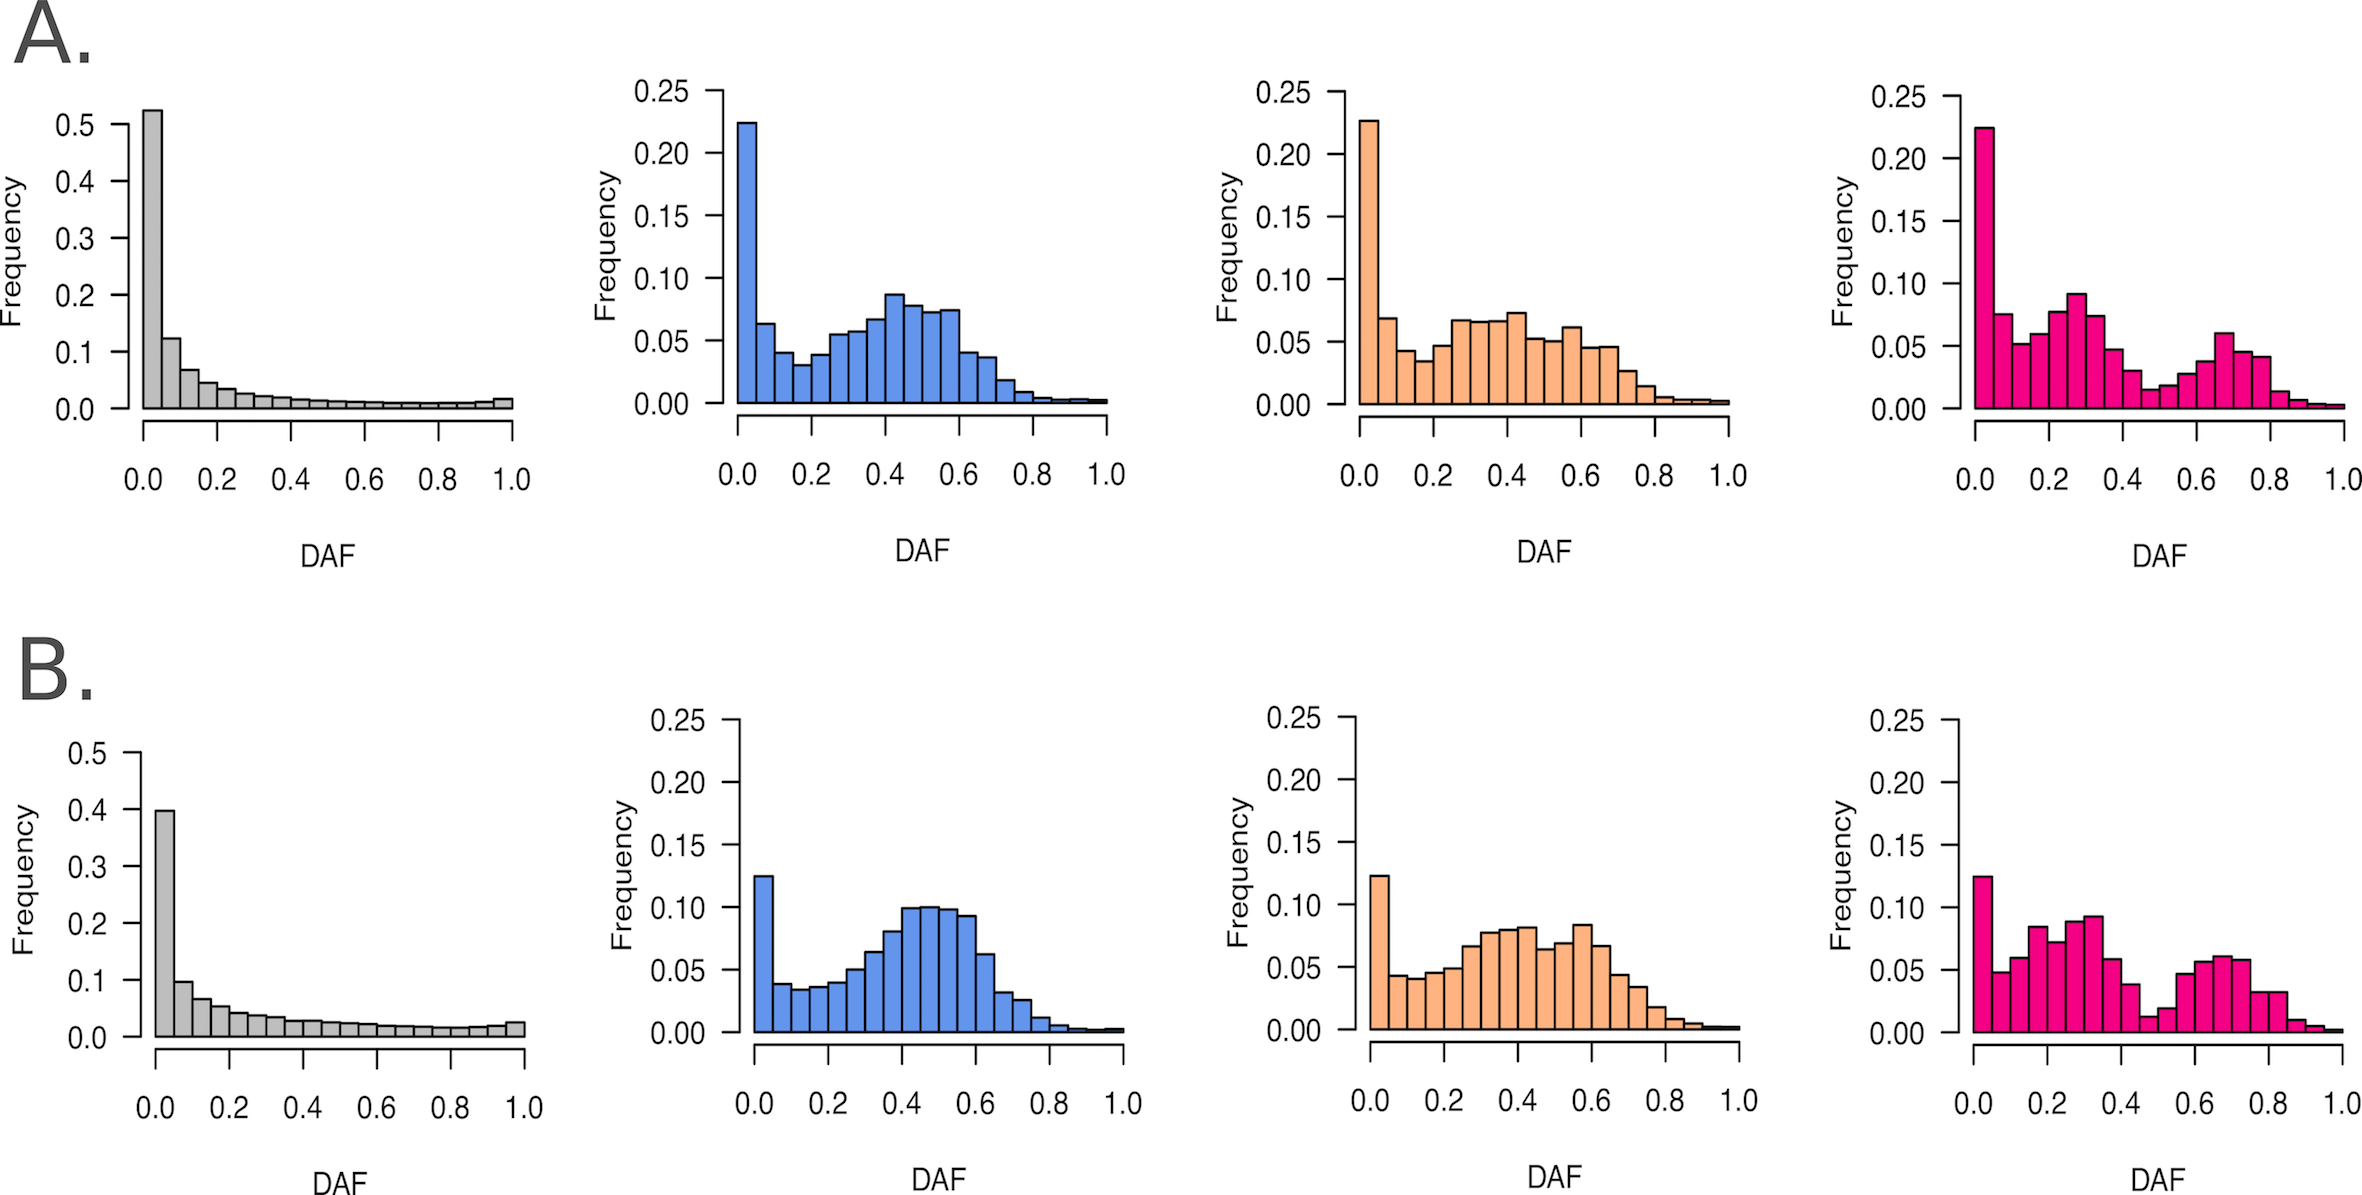
\includegraphics[]{chap2_folder/Figures/Fig5.png}
\caption*{\textbf{Figure 5. Site frequency spectra}\\
SFS in \textbf{A)} LWK population and \textbf{B)} GBR population of background windows (all windows in chromosome 1, in grey), significant windows for $NCD2_{0.5}$ (blue), significant windows for $NCD2_{0.4}$ (orange), and significant windows for $NCD2_{0.3}$ (pink).}
\end{sidewaysfigure}
%%%%%%%%%%%%%%%%%%%%%%%%%%%%%%%%%%%%%%%%%%%%%%%%%%%%%%%%%%%%%%%%%%%%%%%%%%%%%%%%%%%%%%%%%%%%%%%%%%%%%%%%%%%%%%
We also examined whether evidence of selection could be driven by two biological mechanisms other than balancing selection: introgression and gene conversion. The outlier windows are significantly depleted of SNPs annotated as introgressed from Neanderthals (S17 Fig, S1 Text), and significant windows do not show a different proportion of introgressed SNPs from controls, showing that introgression is not a confounding mechanism leading to significant or outlier regions (S7 Fig, S1 text). Finally, the genes overlapped by significant windows are not predicted to be particularly affected by non-homologous gene conversion with neighboring paralogs, with the exception of olfactory receptors (S16 and S19 Figs, S1 Text). Thus, the significant and outlier windows represent a catalog of strong candidate targets of balancing selection in human populations that are not likely to be driven by introgression or gene conversion (S16, S17, S19 Figs, S1 Text).


\subsection{Non-random distribution across the genome}
Significant and outlier windows were not randomly distributed across the genome. Chromosome 6 is the most enriched for signatures of LTBS, contributing 11.2\% of significant windows genome-wide (24.5\% of outlier windows) while having only 6.4\% of analyzed windows (S12 Fig). This is due to the presence of the MHC region, rich in genes with well-supported evidence for balancing selection. In fact, several HLA genes known to be targets of LTBS appear among our outlier windows, i.e, the strongest candidates. For the outlier windows, 10 HLA genes are found in all four populations, most of which have prior evidence for balancing selection (Table 3): \emph{HLA-B},\emph{HLA-C}, \emph{HLA-DPA1}, \emph{HLA-DPB1}, \emph{HLA-DQA1}, \emph{HLA-DQB1}, \emph{HLA-DQB2}, \emph{HLA-DRB1}, \emph{HLA-DRB5}, \emph{HLA-G} (\cite{DeGiorgio2014,Liu2006,Meyer2006,Sanchez-Mazas2007,Solberg2008,Tan2005}).

\subsection{The biological pathways influenced by LTBS}

Although the union of significant windows considering all $tf$ values span on average only 0.51\% of the genome (Table 2), 37.8\% of those windows overlap protein-coding genes. To gain insight on the biological pathways influenced by balancing selection, we focused on protein-coding
genes that contain at least one significant or outlier window (“U” set, Table 2), and investigated the functional categories they belong to.

We found enrichment for 30 GO (Gene Ontology) categories for the significant genes (S2 Table), 22 of which are shared by at least two populations. Three significant categories are driven by olfactory receptor genes (OR), which we could not rule out as artifacts (S1 Text), although they do not appear in the more conservative outlier set of genes (S3 Table). Among the remaining categories, at least half of them are directly related to immune response (e.g.
“type I interferon signaling pathway”, “MHC class I protein complex”, “positive regulation of T cell mediated cytotoxicity”) and 11 are involved in antigen presentation by MHC molecules (e.g. “MHC class I protein complex”, “MHC class II protein complex”, “peptide antigen binding”, among others). For the outlier genes, 27 enriched categories were found, at least 18 of which are immune-related, and 10 of which are directly related to antigen presentation by MHC molecules (S3 Table).

When classical HLA genes are removed from the sets, no categories remain enriched for the outlier genes (S3 Table; but note that this resulted in a small set of 162-192 genes per population, with lower power to detect GO
category enrichment), as in \textcite{DeGiorgio2014}. For the larger set of significant genes, the immune related category “peptide antigen
binding” remains significant in LWK , driven by \emph{TAP1}, \emph{TAP2}, and \emph{HLA-G}, all previously reported candidate targets of balancing selection (\cite{Cagliani2011a,Tan2005}). These results
show the strong influence of the classical HLA genes to signatures of LTBS. However, “extracellular region” and “keratin filament” are enriched in the set of significant genes, in several populations, even after the removal of HLA genes, in agreement with previous findings pointing that balancing selection targets genes related to extracellular and cell-surface
proteins (\cite{Key2014b}).

Nevertheless, for the significant genes only about half of the immune-related enriched categories are directly linked to peptide presentation by MHC molecules. Other categories (e.g. “type I interferon signaling pathway”, “cytokine mediated pathway”, “T cell co-stimulation”, “immune response”), even if they cease to be significantly enriched after the removal of HLA genes (S2 Table), are not strictly composed of HLA genes. 

In order to gain more insight on the importance of non-HLA immune related genes to the outlier set of genes, we verified that the GO categories of 62 outlier genes shared by at least two populations (Table 3) are immune-related, although only 10 HLA genes compose that set (S8 Table). This shows that not only \emph{HLA}-related categories are enriched among the significant genes,
pointing that immune response, in a broader sense, is enriched for LTBS (reviewed in \cite{Key2014b}).

Regarding tissue of expression, among the genes overlapped by significant windows, we found enrichment for genes preferentially expressed in “adrenal” (TSI, p-value=0.003, S5 Table) and “lung” (GBR, p-value=0.004, S5 Table, S1 Text).

%%%%%%%%%%%%%%%%%%%%%%%%%%%%%%%%%%%%%%%%%%%%%%%%%%%%%%
%%%%%%%%%% %%%%%%%%%%%%%%%%%%%%%%%%%%%%%%%%%%%%%%%%%%%
%%%%%%%%%%%%%%%%%%%%%%%%%%%%%%%%%%%%%%%%%%%%%%%%%%%%%%
%%%%%%%%%% %%%%%%%%%%%%%%%%%%%%%%%%%%%%%%%%%%%%%%%%%%%
%%%%%%%%%%%%%%%%%%%%%%%%%%%%%%%%%%%%%%%%%%%%%%%%%%%%%%
%%%%%%%%%% %%%%%%%%%%%%%%%%%%%%%%%%%%%%%%%%%%%%%%%%%%%
%%%%%%%%%%%%%%%%%%%%%%%%%%%%%%%%%%%%%%%%%%%%%%%%%%%%%%
%%%%%%%%%% %%%%%%%%%%%%%%%%%%%%%%%%%%%%%%%%%%%%%%%%%%%

\begin{sidewaystable}[!ht]
\centering
\caption*{\textbf{Table 2. Significant and outlier windows and protein-coding genes across populations}\\
Significant and outliers, see main text.
U, union of all windows found with all target frequencies ($tf$).
}
\label{table2manuscript}
\resizebox{\textwidth}{!}{%
\begin{tabular}{ccccccccccccccccc}
\hline
\rowcolor[HTML]{656565} 
Population & \multicolumn{4}{c}{\cellcolor[HTML]{656565}LWK} & \multicolumn{4}{c}{\cellcolor[HTML]{656565}YRI} & \multicolumn{4}{c}{\cellcolor[HTML]{656565}GBR} & \multicolumn{4}{c}{\cellcolor[HTML]{656565}TSI} \\ \hline
\rowcolor[HTML]{EFEFEF} 
\cellcolor[HTML]{C0C0C0}tf & 0.3 & 0.4 & 0.5 & U & 0.3 & 0.4 & 0.5 & U & 0.3 & 0.4 & 0.5 & U & 0.3 & 0.4 & 0.5 & U \\ \cline{2-17} 
\cellcolor[HTML]{C0C0C0}\begin{tabular}[c]{@{}c@{}}Significant\\  windows\end{tabular} & 5,620 & 5,516 & 4,826 & 7,770 & 6,137 & 5,919 & 5,213 & 8,436 & 5,465 & 6,312 & 5,904 & 8,526 & 5,464 & 6,183 & 5,801 & 8,395 \\
\cellcolor[HTML]{C0C0C0}\begin{tabular}[c]{@{}c@{}}Outlier \\ windows\end{tabular} & 816 & 816 & 816 & 1,139 & 816 & 816 & 816 & 1,142 & 816 & 816 & 816 & 1,131 & 816 & 816 & 816 & 1,163 \\
\cellcolor[HTML]{C0C0C0}\begin{tabular}[c]{@{}c@{}}Significant \\ genes\end{tabular} & 1,037 & 1,003 & 878 & 1,321 & 1,129 & 1,044 & 928 & 1,400 & 967 & 1,025 & 971 & 1,321 & 983 & 1,047 & 1,009 & 1,378 \\
\cellcolor[HTML]{C0C0C0}\begin{tabular}[c]{@{}c@{}}Outlier \\ genes\end{tabular} & 128 & 130 & 147 & 202 & 124 & 120 & 131 & 187 & 107 & 114 & 123 & 172 & 116 & 121 & 137 & 189 \\
\cellcolor[HTML]{C0C0C0}\begin{tabular}[c]{@{}c@{}}Queried\\  windows\end{tabular} & \multicolumn{4}{c}{1,631,372} & \multicolumn{4}{c}{1,631,372} & \multicolumn{4}{c}{1,631,372} & \multicolumn{4}{c}{1,631,372} \\ \hline
\end{tabular}%
}
\end{sidewaystable}

%%%%%%%%%%%%%%%%%%%%%%%%%%%%%%%%%%%%%%%%%%%%%%%%%%%%%%%%%%%%%%%%%%%%%%%%%%%%%%%%%%%%%%%%%%%%%%%%%%%%%%%%%%%%%%%%%%%%%%%%%%%%%%%%%%%%%%%%%%%%%%%%
%%%%TABLE %%% TABLE %%% TABLE %%%% TABLE %%%%%%%TABLE %%% TABLE %%% TABLE %%%% TABLE %%%%%%%TABLE %%% TABLE %%% TABLE %%%% TABLE %%%%%%%TABLE %%
%%%%%%%%%%%%%%%%%%%%%%%%%%%%%%%%%%%%%%%%%%%%%%%%%%%%%%%%%%%%%%%%%%%%%%%%%%%%%%%%%%%%%%%%%%%%%%%%%%%%%%%%%%%%%%%%%%%%%%%%%%%%%%%%%%%%%%%%%%%%%%%%
%%%%%%%%%%%%%%%%%%%%%%%%%%%%%%%%%%%%%%%%%%%%%%%%%%%%%%%%%%%%%%%%
\subsection{Overlap of significant windows across populations}
%%%%%%%%%%%%%%%%%%%%%%%%%%%%%%%%%%%%%%%%%%%%%%%%%%%%%%%%%%%%%%%%
%%%%%%%%%%%%%%%%%%%%%%%%%%%%%%%%%%%%%%%%%%%%%%%%%%%%%%%%%%%%%%%%
Most windows were found to be significant (S20A Fig) or outliers (S20B Fig) in multiple populations. On average 81\% of significant windows in any one population are shared between any two populations, and 69\% of the windows are shared between two populations within the same continent (66\% between African and 71\% between European populations, see S20A Fig). For the more restrictive set of outlier windows, the sharing increased to 87\% between any two populations, and 78\% within continent (75\% of African windows were shared, and 80\% of European (S20B Fig). There was also similar sharing considering $tf$ values separately (S21-S22 Figs).
%%%%%%%%%%%%%%%%%%%%%%%%%%%%%%%%%%%%%%%%%%%%%%%%%%%%%%%%%%%%%%%%
\subsection{The putative function of balanced SNPs}
%%%%%%%%%%%%%%%%%%%%%%%%%%%%%%%%%%%%%%%%%%%%%%%%%%%%%%%%%%%%%%%%
\paragraph{Functional protein-coding sites} To further investigate the differences among outlier and non-outliers (background) windows, we examined the degree to which they overlap exons. On average, 31.2\% of the windows that overlap protein-coding genes overlap their exons, very similar to the 30.8\% for the background distribution (S15 Fig). In fact, significant windows contain a higher (but non-significant) proportion of protein-coding SNPs than background windows (Fig 6A,C).


%%%%%%%%%%%%%%%%%%%%%%%%%%%%%%%%%%%%%%%%%%%%%%%%%%%%%%%%%%%%%%%%%%%%%%%%%%%%%%%%%%%%%%%%%%%%
%%%  Figure 7  %%%
%%%%%%%%%%%%%%%%%%
\begin{figure}[!ht]
\centering
\includegraphics[]{chap2_folder/Figures/Fig6.tiff}
\caption*{\textbf{Figure 6. Enrichment in protein-coding and non-synonymous SNPs}\\ 
Proportion of SNPs that are protein-coding \textbf{(A,C)} and proportion of protein-coding SNPs that are nonsynonymous \textbf{(B,D)} for all SNPs \textbf{(A,B)} or SNPs with intermediate MAF in the significant and background windows \textbf{(C,D)}. NS, nonsynonymous; S, synonymous; C, coding; I, intergenenic. In gray, distribution obtained from 1,000 samplings of a set of windows from the background (see Methods). In orange, significant windows.}
\end{figure}
%%%%%%%%%%%%%%%%%%%%%%%%%%%%%%%%%%%%%%%%%%%%%%%%%%%%%%%%%%%%%%%%%%%%%%%%%%%%%%%%%%%%%%%%%%%%%%%%%%%%%%%%%%%%%%%%%%%%%%%%%%%%%%%%%%%%%%%%%%%%%%%%%%

When these sites are divided as synonymous (putatively neutral) and non-synonymous, significant windows are enriched for non-synonymous SNPs when compared with controls sampled from the background distribution (Fig 6A,C). This is also true when only intermediate frequency alleles are considered (MAF>0.20, Fig 6B,D). Taken together, our results indicate that balancing selection is associated to regions of increased non-synonymous polymorphism.

\paragraph{Regulatory function} It has been suggested that balancing selection may have a particularly important role in maintaining genetic diversity that affects gene expression (\cite{Leffler2013a,Savova2016}). Because the identification of significant and outlier windows is independent from functional annotation, we are in a position to test the hypothesis that LTBS has preferentially targeted regulatory regions. Significant windows were enriched in SNPs that have regulatory functions (Fig 7A, p<0.001), annotated as eQTLs (Regulome Category 1).

Nevertheless, power to annotate a SNP as an eQTL increases with its frequency, so allele frequency must be accounted for. When only SNPs with intermediate frequency alleles are considered, significant windows no longer show a statistical enrichment in eQTLs (Fig 7D); rather, in most populations there is a significant depletion of eQTLs (Fig 7D). Accordingly, we observed a depletion of SNPs overlapping putatively regulatory regions when considering a more inclusive category that depends exclusively on genomic context (rather than on eQTL annotation, RegulomeDB categories 1 and 2, see Methods; Fig 7B-E). Regardless of allele frequency, SNPs in significant windows are enriched in sites with no evidence of a role in gene regulation (RegulomeDB category 7, Fig 7C-F). Although the annotation of each of these RegulomeDB categories is not perfect, these results suggest that balancing selection does not preferentially target, in human populations, sites with a role in gene expression regulation. 
%%%%%%%%%%%%%%%%%%%%%%%%%%%%%%%%%%%%%%%%%%%%%%%%%%%%%%%%%%%%%%%%%%%%%%%%%%%%%%%%%%%%%%%%%%%%
%%%  Figure 7  %%%
%%%%%%%%%%%%%%%%%%
\begin{sidewaysfigure}[!ht]
\centering
\includegraphics[]{chap2_folder/Figures/Fig7.tiff}
\caption*{\textbf{Figure 7. RegulomeDB enrichment analysis for scores 1 and 7}\\
Proportion of SNPs in \textbf{(A,D)} RegulomeDB category 1 (eQTLs), \textbf{(B,E)} RegulomeDB categories 1 and 2 (overlapping a putatively regulatory site) or \textbf{(C,F)} RegulomeDB category 7 (no evidence for regulatory role) for \textbf{(A,B,C)} all SNPs or \textbf{(D,E,F)} SNPs with intermediate MAF in both the significant and background windows. In gray, distribution obtained from 1,000 samplings of a set of windows from the background (see Methods). In orange, significant windows. 
}
\end{sidewaysfigure}
%%%%%%%%%%%%%%%%%%%%%%%%%%%%%%%%%%%%%%%%%%%%%%%%%%%%%%%%%%%%%%%%%%%%%%%%%%%%%%%%%%%%%%%%%%%%%%%%%%%%%%%%%%%%%%%%%%%%%%%%%%%%%%%%%%%%%%%%%%%%%%%%%%


Finally, in agreement with \textcite{Savova2016} we find a modest yet significant enrichment for genes with mono-allelic expression (MAE) among the outlier genes shared by at least two populations (Table 3): 26\% of them are MAE genes, while only 22\% of the non-outliers are MAE (p=0.03, Fisher Exact Test, one-sided).

\subsection{The top candidate genes}
The signatures of long-term balancing selection may not be shared between populations due to changes in selective pressure, which may be important during fast, local adaptation (\cite{DeFilippo2016}). Still, loci with signatures across human populations are more likely to represent old, stable events of balancing selection in human populations.  We considered as “African” those outlier genes resulting from the union of outlier windows for all $tf$ values (Table 2) that are shared between YRI and LWK (but neither or only one of the European populations), and as “European” those that shared between GBR and TSI (but neither or only one of the African populations). Those shared by all four populations were considered as “African and European” (Table 3). Importantly, these designations do not imply that the genes referred to as “African” or “European” in Table 3 are putative targets of LTBS for only one of the continents, as there are power differences between Africa and Europe, particularly for $tf=0.3$ (Fig 3, Table 1, S10 Fig), but rather serve the purpose of quantifying the extent of sharing across populations.

The combined set of “African” (69 genes), “European” (71 genes) and “African and European” (75 genes) contains 213 genes (~1.1\% of all queried genes) (Table 3). When applying the same criteria for the significant windows, the set contains 1,470 genes (~8\% of all queried genes, see S2 Text and S8 Table). We focus the following discussion on the set of 213 outlier genes, since they constitute the most restricted set. Of these, 61 (29\%) have evidence of balancing selection in at least one previous genome-wide analysis (\cite{Andres2009,DeGiorgio2014,Leffler2013a}), and others were detected in individual gene studies (Table 3 and Discussion). Overall, about 70\% of the outlier genes reported here have not been reported as having signatures of LTBS in previous studies.

Obviously, a given window can be significant for more than one $tf$ value. Because our simulations suggest that the $tf$ is informative about the frequency of the balanced allele, we use the lowest $Z_{\mathrm{tf}}$ to assign a $tf$ value to each window (for a given population), providing information on the nature of the SFS skew (S7 Table). For 50\% of the outlier windows, the assigned $tf$ is 0.3, and ~36\% have 0.5 as assigned $tf$; only ~14\% have assigned $tf=0.4$ (S6 Table). 

Based on the p-values of the most extreme window for each of the outlier genes, we were able to rank them. The top 10 genes are highlighted in Table 3. Among the top ten candidates, two (\emph{HLA-DRB5} and \emph{HLA-DQA1}) are related to adaptive immunity, two (\emph{PCDH15} and \emph{NDUFA10}) are related to sensory perception of mechanical stimulus, including sound and two (\emph{PROKR2} and \emph{CPE}) are related to neuropeptide signaling pathway. Six of the top 10 genes (\emph{PROKR2}, \emph{HLA-DQA1}, \emph{CPE}, \emph{HLA-DRB5}, \emph{LUZP2}, and \emph{MYO3A}) have been previously described as having signatures of LTBS in humans (Table 3). The four among them that are novel (\emph{B4GALNT2}, \emph{C1orf101}, \emph{NDUFA10}, and \emph{PCDH15}) are discussed in more detail in the discussion.

%%%%%%%%%%%%%%%%%%%%%%%%%%%
\begin{scriptsize}
\begin{longtable}{ccc}
\caption*{\textbf{Table 3. Outlier genes} All reported genes have are overlapped by at least one outlier window for at least one $tf$ value (Table 2 and Methods). Outliers for both African populations (“African”), for both European populations (“European") or for all four populations ("African \& European"). A version of this table with p-values and assigned $tf$ values is provided in S7 Table. When a gene has been previously reported as having signatures of LTBS, the reference is provided. [A], \textcite{Andres2009}, [D], \textcite{DeGiorgio2014}, [L], \textcite{Leffler2013a}, [S], reported as being under balancing selection in \textcite{Savova2016}, [T] \textcite{Tan2005}. * top 10 most highly ranked genes (for YRI).}\\

\toprule
\rowcolor[HTML]{C0C0C0} 
African & European & African and European \\ \midrule
\textit{ABO\textsuperscript{{[}SG{]}{[}S{]}}} & \textit{AC121757.1} & \textit{APBB1IP	\textsuperscript{{[}D{]}}} \\
\textit{ADAM29} & \textit{ADAM12} & \textit{B4GALNT2**} \\
\textit{AIM1} & \textit{ADRA1D} & \textit{BICD1} \\
\textit{ALDH1L1} & \textit{AL590867.1} & \textit{CAMK1D} \\
\textit{ALK} & \textit{ALG8\textsuperscript{{[}D{]}}} & \textit{CDSN\textsuperscript{{[}D{]}{[}A{]}{[}S{]}}} \\
\textit{ARHGAP8} & \textit{ATP10D} & \textit{CHST11} \\
\textit{ATXN3} & \textit{B3GNTL1} & \textit{CPE\textsuperscript{{[}D{]}}} \\
\textit{BCAR3} & \textit{BICC1\textsuperscript{{[}D{]}}} & \textit{CTNNA3} \\
\textit{C1orf54} & \textit{C1orf222} & \textit{DMBT1		\textsuperscript{{[}D{]}}} \\
\textit{C15orf48} & \textit{CCDC169\textsuperscript{{[}D{]}}} & \textit{EDARADD} \\
\textit{C1orf101*} & \textit{CCDC169-SOHLH2\textsuperscript{{[}D{]}}} & \textit{EGLN3} \\
\textit{C22orf34} & \textit{CDH5} & \textit{ERO1LB} \\
\textit{CCHCR1} & \textit{CEP112\textsuperscript{{[}D{]}}} & \textit{FAM101A} \\
\textit{CELSR1} & \textit{CNR2} & \textit{FAM19A5} \\
\textit{CLDN16} & \textit{CNTNAP2} & \textit{FCER2} \\
\textit{COG6} & \textit{COL4A3\textsuperscript{{[}D{]}}} & \textit{FMN2} \\
\textit{COL25A1} & \textit{CPNE4\textsuperscript{{[}D{]}}} & \textit{GPR137B} \\
\textit{COMMD10} & \textit{CRHR1} & \textit{GPRIN3} \\
\textit{CUBN\textsuperscript{{[}D{]}}} & \textit{CSMD1\textsuperscript{{[}D{]}}} & \textit{HBE1 **} \\
\textit{DIRC3} & \textit{DOK6} & \textit{HBG2 **} \\
\textit{DTNA} & \textit{FRAS1\textsuperscript{{[}D{]}}} & \textit{HIP1} \\
\textit{EPHA6} & \textit{FXN\textsuperscript{{[}D{]}}} & \textit{HLA-B\textsuperscript{{[}A{]}{[}D{]}{[}S{]}}} \\
\textit{EXTL3} & \textit{GABBR2} & \textit{HLA-C		\textsuperscript{{[}D{]}}} \\
\textit{FRMD4B\textsuperscript{{[}D{]}}} & \textit{GNA15} & \textit{HLA-DPA1\textsuperscript{{[}D{]}}} \\
\textit{GPR114} & \textit{GRAMD4} & \textit{HLA-DPB1		\textsuperscript{{[}D{]}}} \\
\textit{GTF2IRD1} & \textit{GRID1} & \textit{HLA-DQA1\textsuperscript{{[}D{]}*}} \\
\textit{HLA-DQA2} & \textit{GRIP1} & \textit{HLA-DQB1\textsuperscript{{[}D{]}}} \\
\textit{IGFBP7\textsuperscript{{[}D,L{]}}} & \textit{HLA-DRA\textsuperscript{{[}D{]}}} & \textit{HLA-DQB2} \\
\textit{IL37{[}S{]}} & \textit{HUS1{[}L{]}} & \textit{HLA-DRB1	
\textsuperscript{{[}D{]}}} \\
\textit{LGALS8\textsuperscript{{[}D,A,S{]}}} & \textit{IDO2} & \textit{HLA-DRB5		\textsuperscript{{[}D{]}}} \\
\textit{LGI2} & \textit{IL18R1\textsuperscript{{[}S{]}}} & \textit{HLA-G} \\
\textit{LUZP222} & \textit{IL1RL1\textsuperscript{{[}S{]}}} & \textit{LRP1B		\textsuperscript{{[}D{]}}} \\
\textit{MLPH} & \textit{ITGA1\textsuperscript{{[}D{]}}} & \textit{MANBA} \\
\textit{MYOM2\textsuperscript{{[}D{]}}} & \textit{KALRN} & \textit{MMP26} \\
\textit{NEDD4L} & \textit{KANSL1} & \textit{BICD1} \\
\textit{NFATC1} & \textit{KDM4C\textsuperscript{{[}D{]}}} & \textit{MROH2A} \\
\textit{NR3C1} & \textit{KL\textsuperscript{{[}D{]}}} & \textit{MYO3A\textsuperscript{{[}D{]}}} \\
\textit{OR52A1} & \textit{KRT83\textsuperscript{{[}D{]}}} & \textit{MYRIP\textsuperscript{{[}D{]}}} \\
\textit{OR6J1} & \textit{LAMC2} & \textit{NCAM2} \\
\textit{PACRG\textsuperscript{{[}D{]}}} & \textit{LDLRAD4\textsuperscript{{[}D{]}}} & \textit{NDUFA10} \\
\textit{PADI2} & \textit{MYO7A} & \textit{OLAH} \\
\textit{PARP15} & \textit{NRXN3} & \textit{PARK2} \\
\textit{PDE10A} & \textit{NSUN4} & \textit{PCDH15*} \\
\textit{PGLYRP4\textsuperscript{{[}D{]}}} & \textit{NTN4\textsuperscript{{[}D{]}}} & \textit{PDSS1} \\
\textit{PRR5-ARHGAP8} & \textit{OAS1{[}S{]}} & \textit{PHACTR2} \\
\textit{PTPRB\textsuperscript{{[}D{]}}} & \textit{ORC5} & \textit{PLCB4\textsuperscript{{[}D{]}}} \\
\textit{PTS} & \textit{OVCH1-AS1} & \textit{PRDM15} \\
\textit{RNF39} & \textit{PGBD5\textsuperscript{{[}D{]}}} & \textit{PREX2\textsuperscript{{[}A{]}}} \\
\textit{RP11-96O20.4} & \textit{PKHD1} & \textit{PROKR2\textsuperscript{{[}L{]}*}} \\
\textit{SFTPD} & \textit{POLR1E\textsuperscript{{[}D{]}}} & \textit{PSORS1C1\textsuperscript{{[}D{]}}} \\
\textit{SGCZ\textsuperscript{{[}D{]}}} & \textit{PPAP2B} & \textit{RIMKLA} \\
\textit{SLC17A5} & \textit{PSMC1} & \textit{RP11-257K9.8} \\
\textit{SLC22A16} & \textit{RASSF6} & \textit{SH3RF3		\textsuperscript{{[}D{]}}} \\
\textit{SLC27A6} & \textit{RBFOX1\textsuperscript{{[}D{]}}} & \textit{SIRPA} \\
\textit{SLC35F2} & \textit{REG4} & \textit{SLA} \\
\textit{SPRR3} & \textit{RUNX2} & \textit{SNX19\textsuperscript{{[}D{]}}} \\
\textit{SPTLC3} & \textit{SEPT11} & \textit{SPAG16} \\
\textit{SQRDL} & \textit{SGCG\textsuperscript{{[}D{]}}} & \textit{SPATA16} \\
\textit{STAU2} & \textit{SKAP2} & \textit{SUCLG2} \\
\textit{STK32A\textsuperscript{{[}D{]}}} & \textit{SLC1A6} & \textit{SV2C} \\
\textit{STXBP6} & \textit{SLC2A9\textsuperscript{{[}D{]} {[}A{]}{[}S{]}}} & \textit{TG} \\
\textit{SUMF1} & \textit{SOHLH2} & \textit{THSD7B\textsuperscript{{[}D{]}}} \\
\textit{TGM6} & \textit{SVEP1} & \textit{TMPRSS2} \\
\textit{TMCO3} & \textit{TCP11L1} & \textit{TMTC2} \\
\textit{TMEM132D} & \textit{TEC} & \textit{UGT2B4\textsuperscript{{[}S{]}{[}T{]}}} \\
\textit{TMEM135} & \textit{TNN} & \textit{WNT7A} \\
\textit{WSCD1} & \textit{TNS1\textsuperscript{{[}A{]}}} & \textit{ZC3H12D} \\
\textit{WWOX} & \textit{TRIM5\textsuperscript{{[}S{]}}} & \textit{ZNF385D} \\
\textit{ZNF331} & \textit{TRPM3} & \textit{ZNF83} \\
\textit{ZNF670} & \textit{VPS8} &  \\
\textit{ZNF695} & \textit{WDYHV1} &  \\
\textit{ZZEF1} & \textit{ZNF254} &  \\ \bottomrule
\end{longtable}
\end{scriptsize}


\afterpage{\FloatBarrier}
%%%%%%%%%%%%%%%%%%%%%%%%%%%%%%%%%%%%%%%%%%%%%%%%

\newpage
\section{Discussion}

\subsection{NCD Method}

We present two new summary statistics, which are simple and fast to compute and to run, and which allow, unlike classical approaches such as Tajima’s \emph{D} (\cite{tajima1989statistical}) or the Mann-Whitney U for comparing local and global SFS (\cite{Andres2009,Nielsen2009}), explicit exploration of different target frequencies - a property also shared by the T1 and T2 tests (\cite{DeGiorgio2014}), albeit in a likelihood framework. We show that the NCD statistics are well powered to detect balancing selection for a complex demographic scenario, such as that of human populations.

The NCD statistics can be used to detect selected regions using null distributions based on neutral simulations (identifying significant windows whose signatures are not expected under neutrality) or by an empirical outlier approach, which allows the investigation of balancing selection when there is limited knowledge on demographic history. Furthermore, $NCD1$ can be used in the absence of a close outgroup species, which extends further the set of possible species. This allows exploring the genomes of species where balancing selection remains completely unexplored.

Many previous and well-supported targets of balancing selection are present in our list of selected genes, but approximately 70\% of the protein-coding genes we identify are novel candidate targets of balancing selection (Table 3). 


%%%%%%%%%%%%%%%%%%%%%%%%%%%%%%%%%%%%%%%%%%%%%%%%%%%%%%%%%%%%
\subsection{Pervasiveness of LTSB in the human genome}
%%%%%%%%%%%%%%%%%%%%%%%%%%%%%%%%%%%%%%%%%%%%%%%%%%%%%%%%%%%%
On average 0.51\% of the windows show, per population, signatures of LTBS that are significant under our simulation-based criteria: we never observed comparable signatures of LTBS with neutral simulations. We showed that these windows are unlikely to be affected by technical or biological artifacts. 

Although the total proportion of the genome under balancing selection may be small, our results show that many genes contain putatively selected regions. For example, under a restrictive criterion of being significant in at least two populations from a continent, 8\% of the protein-coding genes contain a significant window, and 1\% contain an outlier window. Because our statistic is powerful for detecting selection in relatively narrow genomic regions (3kb), it is possible that we are identifying signatures that would not be found when analyzing properties of entire genes or larger genomic regions.

\subsection{Protein-coding and intergenic targets}
Long-term balancing selection is known to maintain both coding -- e.g., \emph{HLA-B}, \emph{HLA-C}, \emph{ABO}
(\cite{Hughes1988,Hughes1989,Segurel2012,Segurel2013}) -- and regulatory diversity -- e.g. \emph{HLA-G}, \emph{UGT2B} (\cite{Tan2005,Sun2011}) (we confirm these targets in Table 3). We are in a particularly good position to quantify the relative proportion of cases of selection acting on coding or regulatory regions in humans. We found no excess of eQTLs within selected windows once the frequency of the alleles is accounted for, and also no evidence for enrichment of regulatory function.

A recent study suggested that there is enrichment for genes with mono-allelic expression (MAE) among those with signatures of balancing selection (\cite{Savova2016}). In agreement with this observation, we found a small but significant enrichment for MAE genes among the outlier genes reported in Table 3 ($p=0.03$, Fisher Exact Test). We note that this overlap would be even
greater if HLA genes had not been excluded by the MAE genes list provided in \textcite{Savova2016}. This result is consistent with the claim for a biological link between balancing selection and MAE
(\cite{Savova2016}). Nevertheless, it remains elusive whether the detection of MAE genes is correlated with allelic frequency, as is the case for eQTLs which could this explain this enrichment.

Although significant windows show a depletion of overlap with protein-coding genes more often than expected by chance, the proportion of the windows overlapping genes that overlap exons is the same for significant and background windows, showing that there is a depletion of introns in the significant windows. Finally, significant and outlier windows show an enrichment for
nonsynonymous SNPs. This result is compatible with two scenarios: (a) direct selection on multiple coding sites or (b) an accumulation of slightly deleterious variants as a bi-product of selection (e.g. \cite{Chun2011}).




%%%%%%%%%%%%%%%%%%%%%%%%%%%%%%%%%%
\subsection{The frequency of the balanced allele(s)}
For both new and previously known targets, an advantage of our method is that it provides an assigned target frequency for each window, and consequently information on the shape of its SFS (Table 3, S7 Table). In some candidate genes – the HLA genes – we know that LTBS has targeted not one, but several sites (\cite{Hughes1988,Hughes1989}). In this case, the theoretical expectation of the shape of the resulting local SFS is unclear. Nevertheless, in loci with a single balanced polymorphism, which we assume may be common outside of the MHC, our simulations suggest that the assigned $tf$ can be informative about the frequency of the balanced allele. Our results indicate that a large proportion of significant windows (50 \%) have minor allele frequencies which lie closer the target allele frequency of 0.3 than to 0.5, as would be expected, for instance, under asymmetric overdominance. This highlights the importance of considering balancing selection regimes with different frequencies of the balanced polymorphism.


%%%%%%%%%%%%%%%%%%%%%%%%%%%%%%%%%%

%%%%%%%%%%%%%%%%%%%%%%%%%%%%%%%%%%
\subsection{The candidate genes}
%%%%%%%%%%%%%%%%%%%%%%%%%%%%%%%%%%

Whereas studies of positive selection show a remarkably low overlap with respect to the genes they identify, with \textcite{Akey2009} reporting that only 14\% of protein-coding loci appear in more than a single study, we identified 61 of the outlier genes (29\%) with evidence of balancing selection in at least one previous genomic analyses (\cite{Andres2009,DeGiorgio2014,Leffler2013a}) (Table 3), and a few other genes detected in individual gene studies (Tables 3 and S7).
This is a reasonable overlap as these studies used both different approaches and datasets. 

Many candidates for balancing selection from previous studies are also identified here. For example, \textcite{Leffler2013a} identified 6 genes with particularly strong evidence of trans-species polymorphisms, 3 of which are outliers in our study (\emph{HUS1}, \emph{PROKR2}, \emph{IGFBP7}; Table 3). Of the 5 genes identified by both \textcite{Andres2009} (an exon-based approach) and \textcite{DeGiorgio2014} (a genome-wide study), 4 are among our outlier genes (\emph{HLA-B}, \emph{CDSN}, \emph{LGALS8}, \emph{SLC2A9}; Table 3), and one (\emph{RCBTB1}) among our significant genes (S8 Table). We find 2 additional genes from \textcite{Andres2009} (\emph{PREX2} and \emph{TNS1}; Table 3) and 53 genes from \textcite{DeGiorgio2014} (Table 3).

Other outlier genes have prior evidence for balancing selection in candidate gene studies. Among the oldest known cases of genetic polymorphisms in humans are the blood-group genes (\cite{Segurel2012,Segurel2013}), including the \emph{ABO} gene, which we also identify (Table 3). \emph{TRIM5} has prior evidence of balancing selection in humans and Old World Monkeys (\cite{Cagliani2010}) and \emph{OAS1} since the split between humans, chimpanzees and gorillas (reviewed in \cite{Fijarczyk2015}); both are involved in innate immune defense. Additional examples include \emph{UGT2B4} - an enzyme that metabolizes steroid hormones and bile acids and is associated to predisposition to breast cancer (\cite{Sun2011}) – and HLA-G – a non-classic HLA gene that has tightly-regulated expression patterns between fetal and adult life (\cite{Tan2005}).

Among the top 10 ranked genes (which we manually checked for undetected duplications and non-homologus gene conversion, S3 Text), we find \emph{B4GALNT2}, \emph{C1orf101}, \emph{NDUFA10}, and \emph{PCDH15}. \emph{NDUFA10} produces a subunit of the enzyme NADH, the largest among the complexes of the
electron-transport chain, and is associated to neurodegenerative diseases such as Leygh’s syndrome, Huntingston’s and Parkinson’s. \emph{C1orf101} is a protein of unknown function which is highly expressed in human testicular tissues (\cite{Petit2015}). \emph{PCDH15} is a protocadherin protein that is essential for normal retinal and cochlear function. Interestingly, this gene shows strong signatures of positive selection in East Asian populations
(\cite{Sabeti2007}). Moreover, two other outlier genes (not among the top 10 ranked genes) are members of the beta-globin cluster and have evidence for recent positive selection in Andean (\emph{HBE1}, \emph{HBG2}) and Tibetan populations (\emph{HBG2}) (\cite{Bigham2010,ROTTGARDT2010,Yi2010}). It is plausible that these genes have been under LTBS in Africa and Europe, and recently been subjected to strong positive selection in non-African populations, a pattern of shift in selective regime recently detected for other loci (e.g. \cite{DeFilippo2016}).

Finally, \emph{B4GALNT2} encodes a blood-group enzyme that has evidence for trans-species polymorphism maintaining two classes of alleles with high divergence, which are responsible for alternative tissue-specific expression patterns (\cite{Linnenbrink2011}). Moreover, variation in this gene in mice seems to be associated with the presence of \emph{Helicobacter} species in the gut (\cite{Staubach2012,Segurel2013}). Finally, a deletion encompassing the first exon of this gene has been described and it is possible that it became fixed in chimpanzees by positive selection (\cite{Perry2008}). To date, our study is the first to confirm evidence of LTBS on \emph{B4GALNT2}  in humans.
%%%%%%%%%%%%%%%%%%%%%%%%%%%%%%%
\section{Conclusions}
We have developed a tool to identify genomic regions under long-term balancing selection that is simple, fast, and has a high degree of sensitivity for different frequencies of the balanced polymorphism. The NCD statistics can be applied to single loci of to the whole genome, in species with sufficient demographic information and those without it, and both in the presence and in the absence of an appropriate outgroup.

Our analyses indicate that, in humans, balancing selection may be shaping variation in about 0.5\% of the genome including at least 1\% of the human protein-coding genes. Because there are so many genes, and since although they affect mostly immunity they also affect other pathways and phenotypes, we provide evidence that balanced polymorphisms appear to be relevant to many biological processes. %check this. see aida's comments on manuscript.

Besides, we provide a catalog of candidate targets of long-term balancing selection, including many completely novel targets. These shall be further investigated, for example, to infer the selective force maintaining the balanced polymorphisms, to determine their phenotypic consequences in present-day human populations. Although about 80\% of windows are shared across populations, the remaining show signatures in individual populations; these will be particularly interesting to investigate their putative influence in subsequent local adaptations through shifts in selective pressure (as in \cite{DeFilippo2016}).


%%%%%%%%%%%%%%%%%%%%%%%%%%%%%%%%%%%%%%%%%%%%%%%%%%%%%%%%%%%%%%%%%%%%%%%%%%%%%%%%%%%%%%%%%%%%%%%%%%%%%%%%%%%%%%%%%%%%%%%%%%%%%%%%%%%%%%%%%%%%%%%%
\section{Materials and Methods} %%%%%%%%%%%%%%%%%%%%%%%%%%%%%%%%%%%%%%%%%%%%%%%%%%%%%%%%%%%%%%%%%%%%%%%%%%%%%%%%%%%%%%%%%%%%%%%%%%%%%%%%%%%%%%%%%
%%%%%%%%%%%%%%%%%%%%%%%%%%%%%%%%%%%%%%%%%%%%%%%%%%%%%%%%%%%%%%%%%%%%%%%%%%%%%%%%%%%%%%%%%%%%%%%%%%%%%%%%%%%%%%%%%%%%%%%%%%%%%%%%%%%%%%%%%%%%%%%%
%%%%%%%%%%%%%%%%%%%%%%%%%%%%%%%%%%%%%%%%%%%%%%%%%%%%%%%%%%%%%%%%%%%%%%%%%%%%%%%%%%%%%%%%%%%%%%%%%%%%%%%%%%%%%%%%%%%%%%%%%%%%%%%%%%%%%%%%%%%%%%%%
\subsection{Simulations}
%%%%%%%%%%%%%%%%%%%%%%%%%%%%%%%%%%%%%%%%%%%%%%%%%%%%%%%%%%%%%%%%%%%%%%%%%%%%%%%%%%%%%%%%%%%%%%%%%%%%%%%%%%%%%%%%%%%%%%%%%%%%%%%%%%%%%%%%%%%%%%%%
%%%%%%%%%%%%%%%%%%%%%%%%%%%%%%%%%%%%%%%%%%%%%%%%%%%%%%%%%%%%%%%%%%%%%%%%%%%%%%%%%%%%%%%%%%%%%%%%%%%%%%%%%%%%%%%%%%%%%%%%%%%%%%%%%%%%%%%%%%%%%%%%

	Performance of $NCD2$ and $NCD1$ was evaluated by extensive simulations with MSMS \parencite{Ewing2010}. The simulations followed a realistic demographic model for African, European and East Asian human populations described in \textcite{Gravel2011}, including the effective populations sizes ($N_{e}$) and migration rates. A generation time of 25 years, a mutation rate of $2.5 * 10^{-8}$ mutations per site \parencite{Nachman2000} and a recombination rate of $1 * 10^{-8}$ were used. The human-chimpanzee split at 6.5 million years ago was added to the model. This was our null demographic model (Fig 2), used to obtain the neutral distributions of NCD.

For simulations with selection, a balanced polymorphism was added to the center of the simulated sequence. The frequency equilibrium ($f_{\mathrm{eq}}$) achieved by the balanced polymorphism was modeled following an overdominant model, as follows. Under the overdominance model, for a bi-allelic locus with alelles A and B, the relative fitnesses of the three genotypes are: $w_{\mathrm{AA}} = 1 - s_{1}$, $w_{\mathrm{AB}} = 1$, and $w_{\mathrm{BB}} = 1 - s_{2}$, where $s_{1}$ and $s_{2}$ are the selection coefficients in the two homozygous genotypes, and the frequency equilibrium ($f_{\mathrm{eq}}$) is equal to $s_{1}/(s_{1}+s_{2})$, as in Equation 4. 

In MSMS, in order to achieve the $f_{\mathrm{eq}}$ we are interested in, we parameterized selection in the following way:  $w_{\mathrm{AB}} = 1+(2N_{e}s)$, $w_{\mathrm{BB}} =1 + [2w_{\mathrm{AB}} - \frac{w_{AB}}{1-f_{\mathrm{eq}}}]$, and $w_{\mathrm{AA}} = 1$, where $N_{e}$ is the effective population size used to scale the coalescent simulations and s is the selection coefficient for the mutant allele (B). The selection coefficient (\emph{s}) was set to 0.01 (the influence of \emph{s} is modest once the frequency equilibrium is reached, as in the case of LTBS). We considered four frequency equilibria: $f_{\mathrm{eq}}$ = 0.2, 0.3, 0.4, 0.5. Simulations with and without selection were run for different sequence lengths (\emph{L}), such that \emph{L} = 3, 6, 12 kb and time of onset of balancing selection (\emph{Tbs}), such that \emph{Tbs} = 1, 3, 5 myr (Fig 2).

%%%%%%%%%%%%%%%%%%%%%%%%%%%%%%%%%%%%%%%%%%%%%%%%%%%%%%%%%%%%%%%%%%%%%%%%%%%%%%%%%%%%%%%%%%%%%%%%%%%%%%%%%%%%%%%%%%%%%%%%%%%%%%%%%%%%%%%%%%%%%%%%
%%%%%%%%%%%%%%%%%%%%%%%%%%%%%%%%%%%%%%%%%%%%%%%%%%%%%%%%%%%%%%%%%%%%%%%%%%%%%%%%%%%%%%%%%%%%%%%%%%%%%%%%%%%%%%%%%%%%%%%%%%%%%%%%%%%%%%%%%%%%%%%%
\subsection{Power analyses} %%%%%%%%%%%%%%%%%%%%%%%%%%%%%%%%%%%%%%%%%%%%%%%%%%%%%%%%%%%%%%%%%%%%%%%%%%%%%%%%%%%%%%%%%%%%%%%%%%%%%%%%%%%%%%%%
%%%%%%%%%%%%%%%%%%%%%%%%%%%%%%%%%%%%%%%%%%%%%%%%%%%%%%%%%%%%%%%%%%%%%%%%%%%%%%%%%%%%%%%%%%%%%%%%%%%%%%%%%%%%%%%%%%%%%%%%%%%%%%%%%%%%%%%%%%%%%%%%
%%%%%%%%%%%%%%%%%%%%%%%%%%%%%%%%%%%%%%%%%%%%%%%%%%%%%%%%%%%%%%%%%%%%%%%%%%%%%%%%%%%%%%%%%%%%%%%%%%%%%%%%%%%%%%%%%%%%%%%%%%%%%%%%%%%%%%%%%%%%%%%%
%
For each set of parameters, 1,000 neutral simulations were compared to 1,000 matching simulations with balancing selection for evaluation of the performance of the NCD statistics. The relationship between the true positive (TPR, the power of the statistic) and false positive (FPR) rates is represented through receiver operating characteristic (ROC) curves. For comparisons between statistics and across demographic scenarios, NCD implementations ($NCD1$ and $NCD2$) and other parameters, the power at the FPR = 0.05 threshold was considered. When comparing performance under a given conditions (e.g. \emph{L} values), power values were averaged across implementations ($NCD1$ and $NCD2$), demographic scenarios (Africa, Europe, Asia), and the other parameters, unless explicitly stated otherwise.

The same simulations and procedures were used to evaluate the comparative performance of the different methods. $NCD2$ and $NCD1$ were run using 3kb windows and \emph{L}=3kb and \emph{Tbs} = 5 myr. They were compared with Tajima’s D (Taj\emph{D}), HKA (\cite{tajima1989statistical,Hudson1987}), and the combined $NCD1$+HKA test (a joint distribution of the two summary statistics) also in 3kb windows. \textcite{DeGiorgio2014} report the performance of T1/T2 based on windows of 100 informative sites upstream and downstream of the target site (on average 13.7 Kb in YRI and 14.7 Kb in CEU). Therefore, we divided 15kb simulations in windows of 100 informative sites and calculated T1 and T2 using BALLET (\cite{DeGiorgio2014}). We selected the highest T1 or T2 value from each simulations to perform the power evaluation.

%%%%%%%%%%%%%%%%%%%%%%%%%%%%%%%%%%%%%%%%%%%%%%%%%%%%%%%%%%%%%%%%%%%%%%%%%%%%%%%%%%%%%%%%%%%%%%%%%%%%%%%%%%%%%%%%%%%%%%%%%%%%%%%%%%%%%%%%%%%%%%%%
%%%%%%%%%%%%%%%%%%%%%%%%%%%%%%%%%%%%%%%%%%%%%%%%%%%%%%%%%%%%%%%%%%%%%%%%%%%%%%%%%%%%%%%%%%%%%%%%%%%%%%%%%%%%%%%%%%%%%%%%%%%%%%%%%%%%%%%%%%%%%%%%
\subsection{Human population genetic data and filtering} %%%%%%%%%%%%%%%%%%%%%%%%%%%%%%%%%%%%%%%%%%%%%%%%%%%%%%%%%%%%%%%%%%%%%%%%%%%%%%%%%%%%%%%
%%%%%%%%%%%%%%%%%%%%%%%%%%%%%%%%%%%%%%%%%%%%%%%%%%%%%%%%%%%%%%%%%%%%%%%%%%%%%%%%%%%%%%%%%%%%%%%%%%%%%%%%%%%%%%%%%%%%%%%%%%%%%%%%%%%%%%%%%%%%%%%%
%%%%%%%%%%%%%%%%%%%%%%%%%%%%%%%%%%%%%%%%%%%%%%%%%%%%%%%%%%%%%%%%%%%%%%%%%%%%%%%%%%%%%%%%%%%%%%%%%%%%%%%%%%%%%%%%%%%%%%%%%%%%%%%%%%%%%%%%%%%%%%%%
\paragraph{Data} We analyzed genome-wide data from the 1000 Genomes Project phase I \parencite{Abecasis2012}. SNPs that were only detected in the high coverage exome sequencing of the 1000G were not considered because the difference in coverage between the low versus high coverage-exclusive SNPs make the exome dataset biased in the sense that coding regions have higher SNP density, potentially biasing our results. 

The genomes of individuals from African and European populations were queried (excluding the recently admixed AWS population), but not those from Asian populations due to lower performance in this population (see “Demography” in the Results section). We considered two African populations (YRI and LWK), and two European populations (GBR and TSI). For comparisons between continents only two European populations were considered (GBR and TSI). 

To equalize sample size, we randomly sampled 50 unrelated individuals from each population \parencite{Key2014}. We used the minor allele frequency (MAF) in the NCD statistics calculations to analyze the folded SFS (Fig 1). This allows us to retain SNPs where the ancestry could not be determined by the 1000G.\nocite{Abecasis2012}

\paragraph{Filtering} Genome analyses require extensive filtering in order to avoid the inclusion of errors that may bias the results. We dedicated extensive efforts to obtain a filtered dataset (see Fig S13). We disregarded positions not present in the 50mer CRG Alignability track \parencite{Derrien2012}, which requires that 50 bp segments should map uniquely (only one region of the genome, allowing up to two mismatches). We filtered out all regions annotated as segmental duplications \parencite{Alkan2009,Cheng2005} and positions that are simple units of repeat detected by the Tandem Repeat Finder \parencite{Benson1999}. We also required that all scanned positions be orthologous to the PanTro2 chimpanzee reference sequence, because $NCD2$ includes FDs. After this filtering, $NCD2$ was calculated for the remaining windows (1,705,970 windows per population). 
%%%%%%%%%%%%%%%%%%%%%%%%%%%%%%%%%%%%%%%%%%%%%%%%%%%%%%%%%%%%%%%%%%%%%%%%%%%%%%%%%%%%%%%%%%%%%%%%%%%%%%%%%%%%%%%%%%%%%%%%%%%%%%%%%%%%%%%%%%%%%%%%
%%%%%%%%%%%%%%%%%%%%%%%%%%%%%%%%%%%%%%%%%%%%%%%%%%%%%%%%%%%%%%%%%%%%%%%%%%%%%%%%%%%%%%%%%%%%%%%%%%%%%%%%%%%%%%%%%%%%%%%%%%%%%%%%%%%%%%%%%%%%%%%%
\subsection{Identifying signatures of LTBS} %%%%%%%%%%%%%%%%%%%%%%%%%%%%%%%%%%%%%%%%%%%%%%%%%%%%%%%%%%%%%%%%%%%%%%%%%%%%%%%%%%%%%%%%%%%%%%%%%%%%
%%%%%%%%%%%%%%%%%%%%%%%%%%%%%%%%%%%%%%%%%%%%%%%%%%%%%%%%%%%%%%%%%%%%%%%%%%%%%%%%%%%%%%%%%%%%%%%%%%%%%%%%%%%%%%%%%%%%%%%%%%%%%%%%%%%%%%%%%%%%%%%%
%%%%%%%%%%%%%%%%%%%%%%%%%%%%%%%%%%%%%%%%%%%%%%%%%%%%%%%%%%%%%%%%%%%%%%%%%%%%%%%%%%%%%%%%%%%%%%%%%%%%%%%%%%%%%%%%%%%%%%%%%%%%%%%%%%%%%%%%%%%%%%%%
Because \emph{L} = 3 Kb yielded the best performance for $NCD2$ for both African and European simulations (see Results, Figs 3, S1, S2), we queried the human population genetic data with sliding windows of \emph{L} = 3 Kb with 1.5 Kb step size. Windows are defined in physical distance since the presence of balancing selection may affect the population-based estimates of recombination rate. Variable positions were categorized as a SNP (if polymorphic in the sample) or a FD (if all humans differ from the chimpanzee); the only exception are polymorphic sites where both allelic states differ from the chimpanzee reference state, as this position was considered both a SNP and a FD. Each population was queried separately, and $NCD2$ was calculated considering three target frequencies: 0.3, 0.4, 0.5. For each queried window, the number of SNPs, FDs, IS, SNP/(FD+1) and $NCD2$ ($tf$ = 0.3, 0.4, 0.5) was computed for each window. 
%%%%%%%%%%%%%%%%%%%%%%%%%%%%%%%%%%%%%%%%%%%%%%%%%%%%%%%%%%%%%%%%%%%%%%%%%%%%%%%%%%%%%%%%%%%%%%%%%%%%%%%%%%%%%%%%%%%%%%%%%%%%%%%%%%%%%%%%%%%%%%%%
%%%%%%%%%%%%%%%%%%%%%%%%%%%%%%%%%%%%%%%%%%%%%%%%%%%%%%%%%%%%%%%%%%%%%%%%%%%%%%%%%%%%%%%%%%%%%%%%%%%%%%%%%%%%%%%%%%%%%%%%%%%%%%%%%%%%%%%%%%%%%%%%
\paragraph{Filtering and correction for number of informative sites (IS)}

Neutrality tests typically place a threshold on the minimum number of informative sites necessary -- e.g. at least 10 IS in \textcite{Andres2009}, and 100 informative sites in \textcite{DeGiorgio2014}. We observe considerable variance in the number of IS per 3 Kb window in the real human genomic data, and find $NCD2$ has high variance when the number of IS is low (S18 Fig). We therefore required that each window has at least 19 (African populations) or 15 (European populations) IS, and the same sets of windows were queried in all 4 populations (Figs S9 and S10). These values where chosen because beyond them $NCD2$ stabilizes (Figs S18 and S19). This final filter resulted in 1,631,372 considered windows  (4\% of the queried windows were excluded) (Fig S13). Furthermore, neutral simulations with different mutation rates were performed in order to retrieve 10,000 simulations for each bin of IS ranging from 4-229 (Africa) and 4-199 (Europe); this range is compatible with the range seen in the actual data. Next, $NCD2$ ($tf$ = 0.3,0.4,0.5) was calculated for all simulations. These simulations per bin of IS allowed both the assignment of significant windows, and the calculation of $Z_{tf}$ (Equation 4, see below).

%%%%%%%%%%%%%%%%%%%%%%%%%%%%%%%%%%%%%%%%%%%%%%%%%%%%%%%%%%%%%%%%%%%%%%%%%%%%%%%%%%%%%%%%%%%%%%%%%%%%%%%%%%%%%%%%%%%%%%%%%%%%%%%%%%%%%%%%%%%%%%%%
%%%%%%%%%%%%%%%%%%%%%%%%%%%%%%%%%%%%%%%%%%%%%%%%%%%%%%%%%%%%%%%%%%%%%%%%%%%%%%%%%%%%%%%%%%%%%%%%%%%%%%%%%%%%%%%%%%%%%%%%%%%%%%%%%%%%%%%%%%%%%%%%
\paragraph{Significant windows}
We defined two sets of windows with signatures of LTBS: the significant windows (obtained based on the simulations) and the outlier windows (obtained based on the
empirical distribution). The significant windows were defined as those that fulfill the criterion whereby the observed $NCD2_{tf}$ value is lower than any of the 10,000 values obtained for simulations with the same number of IS. Based on this criterion, all significant windows have the same \emph{p}-value ($p<0.0001$).

%%%%%%%%%%%%%%%%%%%%%%%%%%%%%%%%%%%%%%%%%%%%%%%%%%%%%%%%%%%%%%%%%%%%%%%%%%%%%%%%%%%%%%%%%%%%%%%%%%%%%%%%%%%%%%%%%%%%%%%%%%%%%%%%%%%%%%%%%%%%%%%%
%%%%%%%%%%%%%%%%%%%%%%%%%%%%%%%%%%%%%%%%%%%%%%%%%%%%%%%%%%%%%%%%%%%%%%%%%%%%%%%%%%%%%%%%%%%%%%%%%%%%%%%%%%%%%%%%%%%%%%%%%%%%%%%%%%%%%%%%%%%%%%%%
\paragraph{Outlier windows}
In order to rank the queried windows and apply an outlier approach, we developed a standardized distance measure between the observed $NCD2_{tf}$ (for the queried window) and the mean of the $NCD2_{tf}$ values for the 10,000 simulations for the matching number of IS. This distance ($Z_{\mathrm{tf}}$) is given by: 

%
\begin{equation}
Z_{tf}=\frac{NCD2_{tf}-\overline{NCD2}_{IS}}{sd_{IS}}
\end{equation}
%

, where $Z_{\mathrm{tf}}$ is the corrected $NCD2_{tf}$ distance by the number of IS, $NCD2_{tf}$ is the $NCD2$ value for the \emph{n}-th empirical window, $NCD2_{IS}$ is the mean $NCD2$ for 10,000 neutral simulations for the corresponding value of IS, and $sd_{IS}$ is the standard deviation of $NCD2$ for 10,000 simulation values with the matching number of IS.

This standardized distance measure takes into account the range of possible values within each IS value, and also the different ranges of values across different target frequencies. Therefore, $Z_{tf}$ allows not only the ranking of all windows for a given $tf$, but also takes into account the residual effect that the number of IS has on $NCD2_{tf}$ (even after filtering for a minimum number of IS, see S11 and S18 Figs) and, finally, allows a comparison between the rankings of a window considering different target frequencies. Once the $Z_{tf}$ scores were calculated, the outlier sets of windows were ranked according to $Z_{0.5}$, $Z_{0.4}$, and $Z_{0.3}$. An empirical \emph{p}-value was attributed to each window based on the $Z_{tf}$ values, and the windows corresponding to the 0.05\% lower tail (816 windows) of the genomic distribution of $Z_{tf}$ values were defined as the “outlier windows”. All outlier windows are contained within the significant windows except four windows in LWK, and one window in TSI.

%
%%%%%%%%%%%%%%%%%%%%%%%%%%%%%%%%%%%%%%%%%%%%%%%%%%%%%%%%%%%%%%%%%%%%%%%%%%%%%%%%%%%%%%%%%%%%%%%%%%%%%%%%%%%%%%%%%%%%%%%%%%%%%%%%%%%%%%%%%%%%%%%%
%%%%%%%%%%%%%%%%%%%%%%%%%%%%%%%%%%%%%%%%%%%%%%%%%%%%%%%%%%%%%%%%%%%%%%%%%%%%%%%%%%%%%%%%%%%%%%%%%%%%%%%%%%%%%%%%%%%%%%%%%%%%%%%%%%%%%%%%%%%%%%%%
\paragraph{Assigned $tf$ values}

As mentioned above, the \emph{p}-values obtained from $Z_{tf}$ can be directly compared across $tf$ values. When a window is an outlier for several $tf$ values, this property allowed an assignment, for each window, of the $tf$ value that minimizes the $NCD2_{tf}$. For the significant and outlier windows, we assigned a $tf$ value as the $tf$ that yields the lowest empirical \emph{p}-value for the window (S6 Table). For the outlier genes in Table 3, a $tf$ value was assigned to a gene by asking: (1) which window overlapping the gene has the lowest \emph{p}-value; and (2) which $tf$ value is associated with the \emph{p}-value in 1. Thus, the assigned $tf$ value for a gene is the assigned $tf$ for the window that has the lowest empirical \emph{p}-value. This was done for each population separately as seen in S7 Table.

%%%%%%%%%%%%%%%%%%%%%%%%%%%%%%%%%%%%%%%%%%%%%%%%%%%%%%%%%%%%%%%%%%%%%%%%%%%%%%%%%%%%%%%%%%%%%%%%%%%%%%%%%%%%%%%%%%%%%%%%%%%%%%%%%%%%%%%%%%%%%%%%
%%%%%%%%%%%%%%%%%%%%%%%%%%%%%%%%%%%%%%%%%%%%%%%%%%%%%%%%%%%%%%%%%%%%%%%%%%%%%%%%%%%%%%%%%%%%%%%%%%%%%%%%%%%%%%%%%%%%%%%%%%%%%%%%%%%%%%%%%%%%%%%%
\paragraph{Coverage}

To test whether the signatures of LTBS are driven by undetected duplications, which can produce mapping error and false SNPs, we analyzed modern human shotgun genome-wide data that has been sequenced to an average coverage per individual between 20x and 30x (\cite{Meyer2012,Prufer2013}). We used an independent dataset because read coverage data is low and cryptic in the 1000G and because putative duplications that affect the SFS must be at appreciable frequency and should be present in other datasets. We considered 12 genomes, two genomes per population, and two populations per continent: Yoruba and San (Africa), French and Sardinian (Europe), Dai and Han Chinese (Asia).

For each sample, we retrieved the positions that have coverage higher than the 97.5\% of the coverage distribution specific for that sample (termed “high coverage” positions). For each window in our analysis for signatures of LTBS, we calculated the proportion of positions having high coverage in at least two samples (pHC), and plot the distributions for different $NCD2$ empirical \emph{p}- values -- i.e, those based on the $Z_{tf}$ scores (S14 Fig). Our significant and outlier windows are not enriched in positions with high coverage in the samples considered herein, but rather the opposite: the significant windows show a significant reduction in the proportion of positions with high coverage when compared with non-significant windows (all Mann-Whitney U test two-tail \emph{p}-value < 0.001).



%%%%%%%%%%%%%%%%%%%%%%%%%%%%%%%%%%%%%%%%%%%%%%%%%%%%%%%%%%%%%%%%%%%%%%%%%%%%%%%%%%%%%%%%%%%%%%%%%%%%%%%%%%%%%%%%%%%%%%%%%%%%%%%%%%%%%%%%%%%%%%%%%%%%%%%%%%%%%%%%%%%%%%%%%%%%%%%%%%%%%%%%%%%%%%%%%%%%%%%%%%%%%%%%%%%%%%%%%%%%%%%%%%%%%%%%%%%%%%%%%%%%%%%%%%%%%%%%%%%%%%%
\subsection{Enrichment Analyses} %%%%%%%%%%%%%%%%%%%%%%%%%%%%%%%%%%%%%%%%%%%%%%%%%%%%%%%%%%%%%%%%%%%%%%%%%%%%%%%%%%%%%%%%%%%%%%%%%%%%%%%%%%%%%%%
%%%%%%%%%%%%%%%%%%%%%%%%%%%%%%%%%%%%%%%%%%%%%%%%%%%%%%%%%%%%%%%%%%%%%%%%%%%%%%%%%%%%%%%%%%%%%%%%%%%%%%%%%%%%%%%%%%%%%%%%%%%%%%%%%%%%%%%%%%%%%%%%
%%%%%%%%%%%%%%%%%%%%%%%%%%%%%%%%%%%%%%%%%%%%%%%%%%%%%%%%%%%%%%%%%%%%%%%%%%%%%%%%%%%%%%%%%%%%%%%%%%%%%%%%%%%%%%%%%%%%%%%%%%%%%%%%%%%%%%%%%%%%%%%%
\paragraph{Gene and Phenotype Ontology}
Whenever a candidate window overlaps a protein coding gene to any extent, this gene is considered a “candidate gene”. This includes windows that fall within intronic regions. GO (gene ontology) and PO (phenotype ontology) enrichment analyses were performed using the software GOWINDA \parencite{Kofler2012}, which avoids common biases that result from gene length (longer genes with more windows have by chance a higher probability of containing a candidate window) and/or gene clustering. We ran the analysis in mode: gene and performed 100,000 simulations for FDR estimation. Significant categories were obtained by considering an FDR<0.05. 
%

GOWINDA was designed for SNP-based analysis so we considered the middle position of every scanned window as the target site. To correct for this, we extended gene coordinates by 1500bp up/down-stream by using the option updownstream1500 in SNP to gene mapping, so we consider the correct coordinates of each window. We used the annotation file (.gtf) and the gene set file for Gene Ontology from Ensembl (http://www.ensembl.org/index.html), and the Phenotype Ontology file from the Human Phenotype Ontology database (http://human-phenotype-ontology.github.io/). 
%
Separate analyses were performed for each population and considering a combination of different sets of genes: 1) different types of candidate windows (outliers \emph{vs} significant windows); 2) different $tf$ (0.5, 0.4 and 0.3); 3) the union of candidate windows for all $tf$; 4) excluding the classical HLA genes with previous evidence of balancing selection (\emph{HLA-B}, \emph{HLA-C}, \emph{HLA-DRB1}, \emph{HLA-DRB5}, \emph{HLA-DPA1}, \emph{HLA-DPA2}, \emph{HLA-DPB1}, \emph{HLA-DPB2}, \emph{HLA-DQB1}, \emph{HLA-DQB2}, \emph{HLA-DQA1}, \emph{HLA-DQA2}).
%
%
%%%%%%%%%%%%%%%%%%%%%%%%%%%%%%%%%%%%%%%%%%%%%%%%%%%%%%%%%%%%%%%%%%%%%%%%%%%%%%%%%%
\paragraph{Enrichment for coding and non-synonymous SNPs} 
%confirmar com o João se ele usou anotação e SNPs do Phase I, ou se foi phase 3.
We used annotation from the 1000 Genomes (\cite{Abecasis2012}) to define coding, intergenic, synonymous and non-synonymous SNPs. Every SNP used in NCD2 calculation and overlapping NCD2-analyzed windows was considered in this analysis. A GOWINDA re-sampling approach as described above was used to perform the enrichment analysis. To control for possible effects of allele frequency on the enrichment for specific features such as eQTLs, a separate analysis only included SNPs at intermediate frequencies (MAF >= 20\%) in each of the four populations.
%
%%%%%%%%%%%%%%%%%%%%%%%%%%%%%%%%%%%%%%%%%%%%%%%%%%%%%%%%%%%%%%%%%%%%%%%%%%%%%%%%%%%%%%%%%%%%%%%%%%%%%%%%%%%%%%%%%%%%%%%%%%%%%%%%%%%%%%%%%%%%%%%%
%%%%%%%%%%%%%%%%%%%%%%%%%%%%%%%%%%%%%%%%%%%%%%%%%%%%%%%%%%%%%%%%%%%%%%%%%%%%%%%%%%%%%%%%%%%%%%%%%%%%%%%%%%%%%%%%%%%%%%%%%%%%%%%%%%%%%%%%%%%%%%%%
\paragraph{RegulomeDB}

To test for enrichment of putatively regulatory sites among targets of balancing selection we used RegulomeDB, which is a SNP-based annotation for known and predicted regulatory elements (\cite{Boyle2012}). Specifically, we considered RegulomeDB scores of 1 (eQTL + $tf$ binding + matched $tf$ motif + matched DNase Footprint + DNase peak) score 2 (TF + binding + matched $tf$ motif + matched DNase Footprint + DNase peak), and 1+2 together (sites that are annotated as eQTL and those that are not), as well as 7 (no regulatory annotation). These represent SNPs with the highest and the lowest evidence for regulatory function, respectively. We also considered score 2 alone (TF binding + matched $tf$ motif + matched DNase Footprint + DNase peak). 
%

For each candidate window we sum the number of SNPs with each score that overlap the window. The expectation in the absence of LTBS is obtained by randomly sampling from the genome the same number of windows as there are with evidence for LTBS (Table 2). This enabled the calculation of an empirical \emph{p}-value of the enrichment of RegulomeDB scores in candidate windows when compared with the empirical background distribution while accounting for the size of each candidate windows set (significance when $p<0.05$). Because we considered the sum of scores across all windows, considering each SNP only once even if it overlapped more than one window, our strategy is insensitive to window length. We conducted similar analyses by considering only alleles found at intermediate frequencies (MAF >= 20\%) as described above.

%%%%%%%%%%%%%%%%%%%%%%%%%%%%%%%%%%%%%%%%%%%%%%%%%%%%%%%%%%%%%%%%%%%%%%%%%%%%%%%%%%%%%%%%%%%%%%%%%%%%%%%%%%%%%%%%%%%%%%%
%%%%%%%%%%%%%%%%%%%%%%%%%%%%%%%%%%%%%%%%%%%%%%%%%%%%%%%%%%%%%%%%%%%%%%%%%%%%%%%%%%%%%%%%%%%%%%%%%%%%%%%%%%%%%%%%%%%%%%%
%%%%%%%%%%%%%%%%%%%%%%%%%%%%%%%%%%%%%%%%%%%%%%%%%%%%%%%%%%%%%%%%%%%%%%%%%%%%%%%%%%%%%%%%%%%%%%%%%%%%%%%%%%%%%%%%%%%%%%%
\paragraph{Immune-related genes}
To specifically test for enrichment for significant genes related to immunity, we used a list of 386 immune-related keywords from the Comprehensive List of Immune Relate Genes from Immport (\url{https://immport.niaid.nih.gov/}) to query the GO categories of the outlier genes. In total, 200 out of our 212 outlier genes have at least one associated GO category, of which 62 have at least one GO category that matches at least one of the keywords on the list and was thus considered to be “immune-related”.

%%%%%%%%%%%%%%%%%%%%%%%%%%%%%%%%%%%%%%%%%%%%%%%%%%%%%%%%%%%%%%%%%%%%%%%%%%%%%%%%%%%%%%%%%%%%%%%%%%%%%%%%%%%%%%%%%%%%%%%%%%%%%%%%%%%%%%%%%%%%%%%%%%%%%%%%%%%%%%%%%%%%%%%%%%%%%%%%%%%%%%%%%%%%%%%%%%%%%%%%%%%%%%%%%%%%%%%%%%%%%%%%%%%%%%%%%%%%%%%%%%%%%%%%%%%%%%%%%%%%%%%%%%%%%%%%%%%%%%%%%%%%%%%%
%\section{Acknowledgements}
%\begin{small}


%We would like to thank Scott Williamson, in memoriam, for having first conceived the idea of this statistic, and Warren Kretszchmar, for doing preliminary analyses on the properties of the NCD statistics. We thank Michael DeGiorgio for assisting with the implementation of the T1 and T2 tests. Additionally, we acknowledge Felix Key, Fabrizio Mafessoni, Kelly Nunes, Philip Klein, Débora YC Brandt, Vitor Aguiar, Joshua Schmidt, Romain Laurent, Jonatas E. Cesar, Sergi Castellano, Michael Dannemann, Bruce Weir, Richard Single, Kay Prüfer, Tatiana T. Torres and Svante Päabo for helpful discussions

%\end{small}
%%%%%%%%%%%%%%%%%%%%%%%%%%%%%%%%%%%%%%%%%%%%%%%%%%%%%%%%%%%%%%%%%%%%%%%%%%%%%%%%%%%%%%%%%%%%%%%%%%%%%%%%%%%%%%%%%%%%%%%%%%%%%%%%%%%%%%%%%%%%%%%%%%%%%%%%%%%%%%%%%%%%%%%%%%%%%%%%%%%%%%%%%%%%%%%%%%%%%%%%%%%%%%%%%%%%%%%%%%%%%%%%%%%%%%%%%%%%%%%%%%%%%%%%%%%%%%%%%%%%%%%%%%%%%%%%%%%%%%%%%%%%%%%%
%% FIGURE %%% FIGURE %%% FIGURE %%% FIGURE %%% FIGURE %%% FIGURE %%% FIGURE %%% FIGURE %%% FIGURE %%% FIGURE %%% FIGURE %%% FIGURE %%% FIGURE %%
%%%%%%%%%%%%%%%%%%%%%%%%%%%%%%%%%%%%%%%%%%%%%%%%%%%%%%%%%%%%%%%%%%%%%%%%%%%%%%%%%%%%%%%%%%%%%%%%%%%%%%%%%%%%%%%%%%%%%%%%%%%%%%%%%%%%%%%%%%%%%%%%%%%%%%%%%%%%%%%%%%%%%%%%%%%%%%%%%%%%%%%%%%%%%%%%%%%%%%%%%%%%%
%% FIGURE %%% FIGURE %%% FIGURE %%% FIGURE %%% FIGURE %%% FIGURE %%% FIGURE %%% FIGURE %%% FIGURE %%% FIGURE %%% FIGURE %%% FIGURE %%% FIGURE %%
%%%%%%%%%%%%%%%%%%%%%%%%%%%%%%%%%%%%%%%%%%%%%%%%%%%%%%%%%%%%%%%%%%%%%%%%%%%%%%%%%%%%%%%%%%%%%%%%%%%%%%%%%%%%%%%%%%%%%%%%%%%%%%%%%%%%%%%%%%%%%%%%%%%%%%%%%%%%%%%%%%%%%%%%%%%%%%%%%%%%%%%%%%%%%%%%%%%%%%%%%%%%%%%%%%%%%%%%%%%%%%%%%%%%%%%%%%%%%%%%%%%%%%%%%%%%%%%%%%%%%%%%%%%%%%%%%%%%%%%%%%%%%%%%%
%% FIGURE %%% FIGURE %%% FIGURE %%% FIGURE %%% FIGURE %%% FIGURE %%% FIGURE %%% FIGURE %%% FIGURE %%% FIGURE %%% FIGURE %%% FIGURE %%% FIGURE %%
%%%%%%%%%%%%%%%%%%%%%%%%%%%%%%%%%%%%%%%%%%%%%%%%%%%%%%%%%%%%%%%%%%%%%%%%%%%%%%%%%%%%%%%%%%%%%%%%%%%%%%%%%%%%%%%%%%%%%%%%%%%%%%%%%%%%%%%%%%%%%%%%%%%%%%%%%%%%%%%%%%%%%%%%%%%%%%%%%%%%%%%%%%%%%%%%%%%%%%%%%%%%%%%%%%%%%%%%%%%%%%%%%%%%%%%%%%%%%%%%%%%%%%%%%%%%%%%%%%%%%%%%%%%%%%%%%%%%%%%%%%%%%%%%
%% FIGURE %%% FIGURE %%% FIGURE %%% FIGURE %%% FIGURE %%% FIGURE %%% FIGURE %%% FIGURE %%% FIGURE %%% FIGURE %%% FIGURE %%% FIGURE %%% FIGURE %%
%%%%%%%%%%%%%%%%%%%%%%%%%%%%%%%%%%%%%%%%%%%%%%%%%%%%%%%%%%%%%%%%%%%%%%%%%%%%%%%%%%%%%%%%%%%%%%%%%%%%%%%%%%%%%%%%%%%%%%%%%
%% FIGURE %%% FIGURE %%% FIGURE %%% FIGURE %%% FIGURE %%% FIGURE %%% FIGURE %%% FIGURE %%% FIGURE %%% FIGURE %%% FIGURE %%% FIGURE %%% FIGURE %%
%%%%%%%%%%%%%%%%%%%%%%%%%%%%%%%%%%%%%%%%%%%%%%%%%%%%%%%%%%%%%%%%%%%%%%%%%%%%%%%%%%%%%%%%%%%%%%%%%%%%%%%%%%%%%%%%%%%%%%%%%%%%%%%%%%%%%%%%%%%%%%%%%%%%%%%%%%%%%%%%%%%%%%%%%%%%%%%%%%%%%%%%%%%%%%%%%%%%%%%%%%%%%%%%%%%%%%%%%%%%%%%%%%%%%%%%%%%%%%%%%%%%%%%%%%%%%%%%%%%%%%%%%%%%%%%%%%%%%%%%%%%%%%%%%%%%%%%%%%%%%%%%%%%%%%%%%%%%%%%%%%%%%%%%%%%%%%%%%%%%%%%
%% FIGURE %%% FIGURE %%% FIGURE %%% FIGURE %%% FIGURE %%% FIGURE %%% FIGURE %%% FIGURE %%% FIGURE %%% FIGURE %%% FIGURE %%% FIGURE %%% FIGURE %%
%%%%%%%%%%%%%%%%%%%%%%%%%%%%%%%%%%%%%%%%%%%%%%%%%%%%%%%%%%%%%%%%%%%%%%%%%%%%%%%%%%%%%%%%%%%%%%%%%%%%%%%%%%%%%%%%%%%%%%%%%%%%%%%%%%%%%%%%%%%%%%%%%%%%%%%%%%%%%%%%%%%%%%%%%%%%%%%%%%%%%%%%%%%%%%%%%%%%%%%%%%%%%%%%%%%%%%%%%%%%%%%%%%%%%%%%%%%%%%%%%%%%%%%%%%%%%%%%%%%%%%%%%%%%%%%%%%%%%%%%%%%%%%%%%%%%%%%%%%%%%%%%%%%%%%%%%%%%%%%%%%%%%%%%%%%%%%%%%%
%% FIGURE %%% FIGURE %%% FIGURE %%% FIGURE %%% FIGURE %%% FIGURE %%% FIGURE %%% FIGURE %%% FIGURE %%% FIGURE %%% FIGURE %%% FIGURE %%% FIGURE %%
%%%%%%%%%%%%%%%%%%%%%%%%%%%%%%%%%%%%%%%%%%%%%%%%%%%%%%%%%%%%%%%%%%%%%%%%%%%%%%%%%%%%%%%%%%%%%%%%%%%%%%%%%%%%%%%%%%%%%%%%%%%%%%%%%%%%%%%%%%%%%%%%%%%%%%%%%%%%%%%%%%%%%%%%%%%%%%%%%%%%%%%%%%%%%%%%%%%%%%%%%%%%%%%%%%%%%%%%%%%%%%%%%%%%%%%%%%%%%%%%%%%%%%%%%%%%%%%%%%%%%%%%%%%%%%%%%%%%%%%%%%%%%%%%
%%%  Figure 7 %%%
%%%%%%%%%%%%%%%%%
%\begin{sidewaysfigure}
%\includegraphics[width=\textwidth, keepaspectratio]{chap2_folder/Figures/Fig7.tiff}
%\caption*{\textbf{Figure 7. Enrichment in protein-coding and non-synonymous SNPs}\\ 
%Proportion of SNPs that are protein-coding \textbf{(A,C)} and proportion of protein-coding SNPs that are nonsynonymous \textbf{(B,D)} for all SNPs \textbf{(A,B)} or SNPs with intermediate MAF in the significant and background windows \textbf{(C,D)}. NS, nonsynonymous; S, synonymous; C, coding; I, intergenenic. In gray, distribution obtained from 1,000 samplings of a set of windows from the background (see Methods). In orange, significant windows.
%}
%\end{sidewaysfigure}
%%%%%%%%%%%%%%%%%%%%%%%%%%%%%%%%%%%%%%%%%%%%%%%%%%%%%%%%%%%%%%%%%%%%%%%%%%%%%%%%%%%%%%%%%%%%%%%%%%%%%%%%%%%%%%%%%%%%%%%%%%%%%%%%%%%%%%%%%%%%%%%%%%%%%%%%%%%%%%%%%%%%%%%%%%%%%%%%%%%%%%%%%%%%%%%%%%%%%%%%%%%%%%%%%%%%%%%%%%%%%%%%%%%%%%%%%%%%%%%%%%%%%%%%%%%%%%%%%%%%%%%%%%%%%%%%%%%%%%%%%%%%%%%%
%% FIGURE %%% FIGURE %%% FIGURE %%% FIGURE %%% FIGURE %%% FIGURE %%% FIGURE %%% FIGURE %%% FIGURE %%% FIGURE %%% FIGURE %%% FIGURE %%% FIGURE %%
%%%%%%%%%%%%%%%%%%%%%%%%%%%%%%%%%%%%%%%%%%%%%%%%%%%%%%%%%%%%%%%%%%%%%%%%%%%%%%%%%%%%%%%%%%%%%%%%%%%%%%%%%%%%%%%%%%%%%%%%%%%%%%%%%%%%%%%%%%%%%%%%%%%%%%%%%%%%%%%%%%%%%%%%%%%%%%%%%%%%%%%%%%%%%%%%%%%%%%%%%%%%%%%%%%%%%%%%%%%%%%%%%%%%%%%%%%%%%%%%%%%%%%%%%%%%%%%%%%%%%%%%%%%%%%%%%%%%%%%%%%%%%%%%

%%%%%%%%%%%%%%%%%%%%%%%%%%%%%%%%%%%%%%%%%%%%%%%%%%%%%%%%%%%%%%%%%%%%%%%%%%%%%%%%%%%%%%%%%%%%%%%%%%%%%%%%%%%%%%%%%%%%%%%%%%%%%%%%%%%%%%%%%%%%%%%%%%%%%%%%%%%%%%%%%%%%%%%%%%%%%%%%%%%%%%%%%%%%%%%%%%%%%%%%%%%%%%%%%%%%%%%%%%%%%%%%%%%%%%%%%%%%%%%%%%%%%%%%%%%%%%%%%%%%%%%%%%%%%%%%%%%%%%%%%%%%%%%%
%% FIGURE %%% FIGURE %%% FIGURE %%% FIGURE %%% FIGURE %%% FIGURE %%% FIGURE %%% FIGURE %%% FIGURE %%% FIGURE %%% FIGURE %%% FIGURE %%% FIGURE %%
%%%%%%%%%%%%%%%%%%%%%%%%%%%%%%%%%%%%%%%%%%%%%%%%%%%%%%%%%%%%%%%%%%%%%%%%%%%%%%%%%%%%%%%%%%%%%%%%%%%%%%%%%%%%%%%%%%%%%%%%%%%%%%%%%%%%%%%%%%%%%%%%%%%%%%%%%%%%%%%%%%%%%%%%%%%%%%%%%%%%%%%%%%%%%%%%%%%%%%%%%%%%%%%%%%%%%%%%%%%%%%%%%%%%%%%%%%%%%%%%%%%%%%%%%%%%%%%%%%%%%%%%%%%%%%%%%%%%%%%%%%%%%%%%
\renewcommand\bibname{References} %need to put 'Bibliografia' in English here.

\renewcommand*{\bibfont}{\footnotesize}
\printbibliography[heading=bibintoc]



%%%%%%%%%%%%%%%%%%%%%%%%%%%%%%%%%%%%%%%%%%%%%%%%%%%%%%%%%%%%%%%%%%%%%%%%%%%%%%%%%%%%%%%%%%%%%%%%%%%%%%%%%%%%%%%%%%%%%%%%%%%%%%%%%%%%%%%%%%%%%%%%%%%%%%%%%%%%%%%%%%%%%%%%%%%%%%%%%%%%%%%%%%%%%%%%%%%%%%%%%%%%%%%%%%%%%%%%%%%%%%%%%%%%%%%%%%%%%%%%%%%%%%%%%%%%%%%%%%%%%%%%%%%%%%%%%%%%%%%%%%%%%%%%
%%%%%%%%%%%%%%%%%%%%%%%%%%%%%%%%%%%%%%
\newpage

%%%%%%%%%%%%%%%%%%%%%%%%%%%%%%%%%%%%%%%%%%%%%%%%%%%%%%%%%%%%%%
%%%%%%%%%%%%%%%%%%%%%%%%%%%%%%%%%%%%%%%%%%%%%%%%%%%%%%%%%%%%%%
%%%%%%%%%%%%%%%%%%%%%%%%%%%%%%%%%%%%%%%%%%%%%%%%%%%%%%%%%%%%%%
\section{Supplementary Text}
%%%%%%%%%%%%%%%%%%%%%%%%%%%%%%%%%%%%%%%%%%%%%%%%%%%%%%%%%%%%%%
%%%%%%%%%%%%%%%%%%%%%%%%%%%%%%%%%%%%%%%%%%%%%%%%%%%%%%%%%%%%%%
%%%%%%%%%%%%%%%%%%%%%%%%%%%%%%%%%%%%%%%%%%%%%%%%%%%%%%%%%%%%%%
\subsection{S1 Text: Additional analyses for significant and outlier windows and genes}

\begin{footnotesize}
\subsubsection{Ruling out possible biological confounding factors}




In all the analyses below, the set of significant or outlier windows (or genes) consists on the union of windows or genes overlapped by them considering all $tf$ values.


\subsubsection{Neanderthal introgression}

\paragraph{Background} Genomic segments that contain introgressed haplotypes from archaic human forms (\cite{Meyer2012,Prufer2013}) have, on average, older TMRCA and higher diversity than the rest of the genome. In the absence of positive (or balancing) selection, though, introgressed segments are not expected to reach intermediate frequencies and contribute to the significant and outlier windows defined in the main paper.

\paragraph{Results} Accordingly, the significant and outlier windows in European populations are not enriched in putatively introgressed SNPs (defined as those with an allele absent in the Africans, shared between Europeans and Neanderthals, and that fall in previously identified introgressed regions (Vernot and Akey, 2014) (S17 Fig and Methods in main paper). In fact, the outlier windows are significantly depleted of introgressed SNPs (S17 Fig). 

\paragraph{Methods} We tested the enrichment of Neanderthal introgression among candidate windows in TSI and GBR by using the resampling approach described for RegulomeDB functional enrichment analysis. Putative Neanderthal-introgressed SNPs were ascertained by considering SNPs that overlap annotated Neanderthal introgressed haplotypes in (\cite{Vernot2014}) and that in the 1000 genomes data show a derived allele shared between TSI/GBR and Neanderthals and absent in YRI and LWK (\cite{Abecasis2012}). The remaining SNPs overlapping scanned windows were considered as non-introgressed.

\subsubsection{Non-homologous gene conversion}

\paragraph{Results and Methods} We also investigated the possibility of non-homologous gene conversion, which is another biological phenomenon that may increase diversity. To do so, for each significant or outlier gene (see Table 2 in main text) we analyzed the distribution of the number of paralogs that reside on the same chromosome. Significant genes show no tendency towards having more paralogs on the same chromosome than all autosomal genes (see S16 Fig), showing that this is not a general issue. In both cases, more than 60\% of the genes have no paralogs on the same chromosome (S16 Fig). 
We nevertheless singled out olfactory receptor (OR) genes (see below), which often appear in tandem and may undergo gene conversion. Unlike the other significant and background genes, more than 80\% of the OR genes present in all populations for at least one $tf$ value have at least one paralog on the same chromosome (S19 Fig). Thus, non-homologous gene conversion does not appear to be a general issue among significant genes, with the exception of the OR genes. 

\subsubsection{Olfactory receptor genes}

Among the windows believed to have less false positive candidates to LTBS, only two OR genes are present: \emph{OR52A1} and \emph{OR6J1} (Table 3). Although patterns compatible with overdominance have been reported for human olfactory receptor activity genes (\cite{Alonso2008}), we cannot rule out that the enrichment signature detected in the genes pertaining to the olfactory receptor (OR) gene family is due to paralogous gene conversion (S19 Fig). Moreover, OR52A1 has 10 paralogues on the same chromosome, and OR6J1 has 1 (Table 3). We therefore recommend that the results concerning OR genes be interpreted with caution.

\subsubsection{Phenotype Ontology Analyses}

\paragraph{Results} A phenotype ontology analysis uncovered “abnormality of the sclera” as the only significant category in YRI, and no significant categories appear in the other three populations analyzed (S4 Table).

\paragraph{Methods} See Methods section in main paper (“Gene and phenotype ontology”).

\subsubsection{Tissue-specific expression}

\paragraph{Results} Interestingly, though, when we perform enrichment analysis among significant windows for tissue-specific expression, we find that targets of LTBS are significantly enriched in genes that are highly expressed in adrenal gland in both TSI and in the lung in GBR European populations (S5 Table). These results are mirrored in African populations when considering outlier windows, albeit the results are not significant. 

\paragraph{Methods} We performed an enrichment analysis using genes showing tissue-specific expression also using GOWINDA, with the same parameters and strategy described above, except here we only considered two criteria for defining different sets in each population: 1) different ascertainment of candidate windows (outlier vs significant); 2) the union of windows for different target frequencies. We used Illumina BodyMap 2.0 (\cite{Derrien2012}) expression data for 16 different tissues, and developed a tissue-specific expression metric that considers genes that are significantly higher expressed in a particular tissue when compared to the remaining 15 tissues using the DESeq package (\cite{Anders2010}). 

%%%%%%%%%%%%%%%%%%%%%%%%%%%%%%%%%%%%%%%%%%%%%%%%%%%%%%%%%%%%%%

\subsection{S2 Text: A set of significant genes}

We considered the union of significant genes (between 1,321 and 1,400 genes for each population, Table 2), and defined as “African” those shared by YRI and LWK and neither or only one of the European populations, as “European” those shared by GBR and TSI and neither or only one of the African populations, and as ‘African and European’ those shared by all four populations. This resulted in 1,051 genes shared between LWK and YRI and 1,089 shared between GBR and TSI. In total, this amounts to 1,470 genes ($\sim8$\% of all queried genes): 670 are considered as “African and European”, 381 are considered as “African” and 419 are considered as “European”. These genes are presented in S8 Table.

%%%%%%%%%%%%%%%%%%%%%%%%%%%%%%%%%%%%%%%%%%%%%%%%%%%%%%%%%%%%%%

\subsection{S3 Text: Manual verification of reliability of SNPs contained in four of the outlier genes}

\subsubsection{Description}

In the main text, we mention that among the top 10 outlier genes from Table 3 (considering the p-values for YRI), 6 have been reported previously as having signatures of LTBS: \emph{PROKR2} (\cite{Leffler2013a}), \emph{HLA-DQA1} (\cite{DeGiorgio2014}), \emph{CPE} (\cite{DeGiorgio2014}), \emph{HLA-DRB5} (\cite{DeGiorgio2014}), \emph{LUZP2} (\cite{DeGiorgio2014}), and \emph{MYO3A} (\cite{Kummerfeld2005,DeGiorgio2014}) (Tables 3 and S7). %fix refs

Thus, the novel top candidates are: \emph{B4GALNT2} (Beta-1,4-N-Acetyl-Galactosaminyl Transferase 2), \emph{C1orf101} (Chromosome 1 Open Reading Frame 101),  \emph{NDUFA10} (NADH-Ubiquinone Oxidoreductase 42 KDa Subunit), and \emph{PCDH15} (Protocadherin-Related 15). In the main text, we discuss these genes in more detail, given that they have extreme signatures of LTBS shared across populations. 

In order to certify that these genes have genuine extreme signatures of LTBS due to balancing selection, and not: (a) bad SNP calls by collapsed reads of duplicates, and (b) non-homologous gene conversion between close paralogs, we performed a manual verification using BLAT (\url{http://www.ensembl.org/Multi/Tools/Blast?db=core}).

\subsubsection{Methods}

For each gene, the corresponding FASTA sequence was taken from the hg19 reference genome and queried in BLAT. We only considered the top 100 hits for each gene. For each of the 100 hits, positions that coincide with a SNP position for the gene in the Phase 1 1000 Genomes data set (\cite{Abecasis2012}) were manually verified. If the position is a match between the query and the hit, i.e, both have the same variant in the SNP position, this SNP is considered a match. If the position is a mismatch between the query and the hit, i.e, query and hit have different variants in the SNP position, this SNP is considered a mismatch. 

A mismatched SNP could either have the alternate allele in the hit (alternate mismatch*) or an allele which is not the alternate allele in the 1000 G data set (simple mismatch). Further, we considered as more relevant and likely problematic those SNPs that not only are classified as alternate mismatch, but have somewhat intermediate frequencies ($>0.10$). Results are provided for each gene separately, below. Location of the gene is provided, for reference.

\subsubsection{Results}

\paragraph{B4GALNT2}

\paragraph{Description} Position: chr17:47203660-47211160 (7,500 bp in total).
In total, 96 SNPs in our filtered data (see Methods in main). Roughly 36 of them have somewhat intermediate frequencies.

\paragraph{BLAT} After looking at all hits, we found three alternate mismatch SNPs. Only two of them have intermediate frequency: rs78050610,rs11654406), while the other is a singleton (rs140853454).

\paragraph{Conclusion} Roughly 94 intermediate SNPs remain for this gene, making it thus unlikely that its signatures are dependent on problematic SNPs.

\medskip
\paragraph{NDUFA10}

\paragraph{Description} Position: chr2:240850012-240854512 (4,500 bp in total). 
In total, 74 SNPs in our filtered data set (see Methods in main). Roughly 41 are intermediate in frequency in most Afr and Eur populations.

\paragraph{BLAT} After looking at all hits, we found two alternate mismatch SNPs, one of which is intermediate frequency (rs6759128) and the other is low to intermediate (rs28429725). 

\paragraph{Conclusion} Roughly 29 intermediate SNPs remain for this gene, making it thus unlikely that its signatures are dependent on problematic SNPs.

\medskip

\paragraph{PCDH15}

\paragraph{Description} Position: chr10:56902047-56911047 (9,000bp in total)
145 SNPs in our filtered data set (see Methods in main), roughly 63 at intermediate frequency.

\paragraph{BLAT} After looking at all hits, we found 1 alternate mismatch SNP (rs188658080), which has verylow frequency in all populations or is absent for some populations (considering only African and European populations).

\paragraph{Conclusion} Although this SNP is likely unreliable, it has low frequency. Coupled with the fact that only this position clearly appears to be problematic, we concluded that the signature observed for this gene is reliable. 

\medskip

\paragraph{C1orf101}

\paragraph{Description} Position: chr1: 244,617,679-244,804,479 (10,500 pb in total), 143 SNPs, roughly 76 at intermediate frequency.

\paragraph{BLAT} After looking at all hits, we found 19 alternate mismatch SNPs. This seemed to be a potentially problematic candidate for LTBS, so we looked at in in further detail. Of the 19 alternate mismatch SNPs, between 7 and 12 have intermediate frequency. They are listed below.

Alternate mistmatch SNPs for \emph{C1orf101} (the ones with * have intermediate frequency and are thus more likely to be sources of bias for observed $NCD2$ values):
rs3003250, rs3005972, rs3005973, rs138545291 (singleton), rs114536159, rs142620294, rs189591539(singleton), rs3003251*, rs3005938*, rs3005945*, rs3005947*, rs3005957*, rs3005958*, rs3005968*, rs3005969*, rs3005971*, rs3005975*, rs7538776*, rs9429008 *

Given that several SNPs for this gene are likely problematic (alternate mismatch with intermediate frequencies, we thus recalculated NCD2 for the windows that overlap this gene, after removing those SNPs. We removed the 19 SNPs (including the low/high frequency ones and singletons) from our data set (Methods in main), and recalculated $NCD2_{0.5}$ for the six outlier windows (Table 2) that overlap this gene for YRI. The six outlier windows that overlapped this gene have zero FDs. For the first of the six window, the removal of the problematic SNPs resulted in it going from 19 to 17 SNPs (IS=17), so it does not fulfill our criteria of having at least 19 IS in Africa (see Methods in main). The second windows goes from having 22 to 19 IS. It passes the "significance criterion" (simulation based $p<0.0001$) and has $Z_{tf}$ value within the observed range for outlier windows. 

\paragraph{Conclusion} 19 SNPs are alternate mismatches, and 7-12 also have intermediate frequencies in most African and European populations. Even if all (19) SNPs are removed and $NCD2_{0.5}$ is re-calculated, at least one window remains as significant and probably outlier, demonstrating that this gene is likely a true positive. Moreover, there is an entire an entire range of the query (between positions 8,000-10,500) for which there are no hits, and this range contains 37 SNPs (around 12 intermediate frequency), further supporting the signatures observed for this gene. 

\end{footnotesize}
%%%%%%%%%%%%%%%%%%%%%%%%%%%%%%%%%%%%%%%%%%%%%%%%%%%%%%%%%%%
%%%%%%%%%%%%%%%%%%%%%%%%%%%%%%%%%%%%%%%%%%%%%%%%%%%%%%%%%%%%%%
%%%%%%%%%%%%%%%%%%%%%%%%%%%%%%%%%%%%%%%%%%%%%%%%%%%%%%%%%%%%%%
\section{Supplementary Tables}
%%%%%%%%%%%%%%%%%%%%%%%%%%%%%%%%%%%%%%%%%%%%%%%%%%%%%%%%%%%%%%
%%%%%%%%%%%%%%%%%%%%%%%%%%%%%%%%%%%%%%%%%%%%%%%%%%%%%%%%%%%%%%
%%%%%%%%%%%%%%%%%%%%%%%%%%%%%%%%%%%%%%%%%%%%%%%%%%%%%%%%%%%%%%
\begin{scriptsize}
\begin{longtable}{lllllllll}
\caption*{\textbf{S1-A Table. Power analyses based on simulations (Africa).} Reported values are for simulations following African demographic scenarios (see Methods). $f_{\mathrm{eq}}$, frequency equilibrium used in the simulations; target frequency is the $tf$ value used in $NCD1$ and $NCD2$; \emph{Tbs}, time since onset of balancing selection; \emph{L}, length of the simulated sequence. Reported values are always for a false positive rate of 0.05.}\\
%\begin{tabular}
\cline{4-9}
\multicolumn{3}{l}{} & \multicolumn{3}{c}{\cellcolor[HTML]{C0C0C0}\textit{NCD2}} & \multicolumn{3}{c}{\cellcolor[HTML]{C0C0C0}\textit{NCD1}} \\ \cline{4-9} 
\multicolumn{3}{l}{} & \multicolumn{6}{c}{\cellcolor[HTML]{9B9B9B}\textbf{Target Frequency}} \\
\cellcolor[HTML]{9B9B9B}\textit{\textbf{Tbs}} & \cellcolor[HTML]{9B9B9B}\textit{\textbf{$f_{\mathrm{eq}}$}} & \cellcolor[HTML]{9B9B9B}\textit{\textbf{L}} & \textbf{0.5} & \textbf{0.4} & \textbf{0.3} & \textbf{0.5} & \textbf{0.4} & \textbf{0.3} \\
\cellcolor[HTML]{C0C0C0}5 & \cellcolor[HTML]{C0C0C0}0.5 & \cellcolor[HTML]{C0C0C0}3 & 0.959 & 0.944 & 0.835 & 0.929 & 0.911 & 0.393 \\
\cellcolor[HTML]{C0C0C0}5 & \cellcolor[HTML]{C0C0C0}0.5 & \cellcolor[HTML]{C0C0C0}6 & 0.917 & 0.885 & 0.728 & 0.903 & 0.847 & 0.392 \\
\cellcolor[HTML]{C0C0C0}5 & \cellcolor[HTML]{C0C0C0}0.5 & \cellcolor[HTML]{C0C0C0}12 & 0.829 & 0.789 & 0.548 & 0.846 & 0.772 & 0.325 \\
\cellcolor[HTML]{C0C0C0}5 & \cellcolor[HTML]{C0C0C0}0.4 & \cellcolor[HTML]{C0C0C0}3 & 0.939 & 0.935 & 0.886 & 0.886 & 0.894 & 0.674 \\
\cellcolor[HTML]{C0C0C0}5 & \cellcolor[HTML]{C0C0C0}0.4 & \cellcolor[HTML]{C0C0C0}6 & 0.871 & 0.860 & 0.790 & 0.838 & 0.819 & 0.651 \\
\cellcolor[HTML]{C0C0C0}5 & \cellcolor[HTML]{C0C0C0}0.4 & \cellcolor[HTML]{C0C0C0}12 & 0.742 & 0.726 & 0.612 & 0.745 & 0.717 & 0.534 \\
\cellcolor[HTML]{C0C0C0}5 & \cellcolor[HTML]{C0C0C0}0.3 & \cellcolor[HTML]{C0C0C0}3 & 0.895 & 0.908 & 0.929 & 0.717 & 0.801 & 0.836 \\
\cellcolor[HTML]{C0C0C0}5 & \cellcolor[HTML]{C0C0C0}0.3 & \cellcolor[HTML]{C0C0C0}6 & 0.776 & 0.796 & 0.833 & 0.659 & 0.709 & 0.794 \\
\cellcolor[HTML]{C0C0C0}5 & \cellcolor[HTML]{C0C0C0}0.3 & \cellcolor[HTML]{C0C0C0}12 & 0.572 & 0.597 & 0.638 & 0.509 & 0.570 & 0.663 \\
\cellcolor[HTML]{C0C0C0}3 & \cellcolor[HTML]{C0C0C0}0.5 & \cellcolor[HTML]{C0C0C0}3 & 0.911 & 0.882 & 0.681 & 0.855 & 0.797 & 0.236 \\
\cellcolor[HTML]{C0C0C0}3 & \cellcolor[HTML]{C0C0C0}0.5 & \cellcolor[HTML]{C0C0C0}6 & 0.856 & 0.809 & 0.574 & 0.854 & 0.770 & 0.266 \\
\cellcolor[HTML]{C0C0C0}3 & \cellcolor[HTML]{C0C0C0}0.5 & \cellcolor[HTML]{C0C0C0}12 & 0.727 & 0.666 & 0.410 & 0.768 & 0.678 & 0.232 \\
\cellcolor[HTML]{C0C0C0}3 & \cellcolor[HTML]{C0C0C0}0.4 & \cellcolor[HTML]{C0C0C0}3 & 0.878 & 0.864 & 0.759 & 0.781 & 0.783 & 0.557 \\
\cellcolor[HTML]{C0C0C0}3 & \cellcolor[HTML]{C0C0C0}0.4 & \cellcolor[HTML]{C0C0C0}6 & 0.803 & 0.785 & 0.678 & 0.770 & 0.753 & 0.527 \\
\cellcolor[HTML]{C0C0C0}3 & \cellcolor[HTML]{C0C0C0}0.4 & \cellcolor[HTML]{C0C0C0}12 & 0.659 & 0.621 & 0.500 & 0.654 & 0.629 & 0.441 \\
\cellcolor[HTML]{C0C0C0}3 & \cellcolor[HTML]{C0C0C0}0.3 & \cellcolor[HTML]{C0C0C0}3 & 0.749 & 0.774 & 0.811 & 0.561 & 0.640 & 0.706 \\
\cellcolor[HTML]{C0C0C0}3 & \cellcolor[HTML]{C0C0C0}0.3 & \cellcolor[HTML]{C0C0C0}6 & 0.628 & 0.648 & 0.700 & 0.526 & 0.570 & 0.658 \\
\cellcolor[HTML]{C0C0C0}3 & \cellcolor[HTML]{C0C0C0}0.3 & \cellcolor[HTML]{C0C0C0}12 & 0.425 & 0.456 & 0.509 & 0.388 & 0.443 & 0.536 \\
\cellcolor[HTML]{C0C0C0}1 & \cellcolor[HTML]{C0C0C0}0.5 & \cellcolor[HTML]{C0C0C0}3 & 0.419 & 0.336 & 0.159 & 0.389 & 0.321 & 0.087 \\
\cellcolor[HTML]{C0C0C0}1 & \cellcolor[HTML]{C0C0C0}0.5 & \cellcolor[HTML]{C0C0C0}6 & 0.356 & 0.283 & 0.107 & 0.395 & 0.294 & 0.086 \\
\cellcolor[HTML]{C0C0C0}1 & \cellcolor[HTML]{C0C0C0}0.5 & \cellcolor[HTML]{C0C0C0}12 & 0.273 & 0.217 & 0.100 & 0.359 & 0.268 & 0.096 \\
\cellcolor[HTML]{C0C0C0}1 & \cellcolor[HTML]{C0C0C0}0.4 & \cellcolor[HTML]{C0C0C0}3 & 0.372 & 0.338 & 0.247 & 0.348 & 0.340 & 0.185 \\
\cellcolor[HTML]{C0C0C0}1 & \cellcolor[HTML]{C0C0C0}0.4 & \cellcolor[HTML]{C0C0C0}6 & 0.305 & 0.278 & 0.206 & 0.355 & 0.324 & 0.195 \\
\cellcolor[HTML]{C0C0C0}1 & \cellcolor[HTML]{C0C0C0}0.4 & \cellcolor[HTML]{C0C0C0}12 & 0.252 & 0.232 & 0.156 & 0.304 & 0.274 & 0.174 \\
\cellcolor[HTML]{C0C0C0}1 & \cellcolor[HTML]{C0C0C0}0.3 & \cellcolor[HTML]{C0C0C0}3 & 0.229 & 0.239 & 0.280 & 0.194 & 0.249 & 0.279 \\
\cellcolor[HTML]{C0C0C0}1 & \cellcolor[HTML]{C0C0C0}0.3 & \cellcolor[HTML]{C0C0C0}6 & 0.190 & 0.203 & 0.233 & 0.210 & 0.232 & 0.277 \\
\cellcolor[HTML]{C0C0C0}1 & \cellcolor[HTML]{C0C0C0}0.3 & \cellcolor[HTML]{C0C0C0}12 & 0.142 & 0.150 & 0.169 & 0.159 & 0.182 & 0.219 \\ \hline
\end{longtable}
\end{scriptsize}

%%%%%%%%%%%%%%%%%%%%%%%%%%%%%%%%%%%%%%%%%%%%%%%%%%%%%%%%%%%%%%%%%%%%%%%%%%%%%%%%%%%%%%%%%
\begin{scriptsize}
\begin{longtable}{lllllllll}
\caption*{\textbf{S1-B Table. Power analyses based on simulations (Europe).} Reported values are for simulations following European demographic scenarios (see Methods). $f_{\mathrm{eq}}$, frequency equilibrium used in the simulations; target frequency is the $tf$ value used in $NCD1$ and $NCD2$; \emph{Tbs}, time since onset of balancing selection; \emph{L}, length of the simulated sequence. Reported values are always for a false positive rate of 0.05.} \\
%\begin{tabular}
\cline{4-9}

\multicolumn{3}{c}{} & \multicolumn{3}{c}{\cellcolor[HTML]{C0C0C0}\textit{NCD2}} & \multicolumn{3}{c}{\cellcolor[HTML]{C0C0C0}\textit{NCD1}} \\ \cline{4-9} 
\multicolumn{3}{c}{} & \multicolumn{6}{c}{\cellcolor[HTML]{9B9B9B}\textbf{Target Frequency}} \\
\cellcolor[HTML]{9B9B9B}\textit{\textbf{Tbs}} & \cellcolor[HTML]{9B9B9B}\textit{\textbf{feq}} & \cellcolor[HTML]{9B9B9B}\textit{\textbf{L}} & \textbf{0.5} & \textbf{0.4} & \textbf{0.3} & \textbf{0.5} & \textbf{0.4} & \textbf{0.3} \\
\cellcolor[HTML]{C0C0C0}5 & \cellcolor[HTML]{C0C0C0}0.5 & \cellcolor[HTML]{C0C0C0}3 & 0.968 & 0.951 & 0.835 & 0.921 & 0.846 & 0.197 \\
\cellcolor[HTML]{C0C0C0}5 & \cellcolor[HTML]{C0C0C0}0.5 & \cellcolor[HTML]{C0C0C0}6 & 0.941 & 0.907 & 0.747 & 0.916 & 0.871 & 0.234 \\
\cellcolor[HTML]{C0C0C0}5 & \cellcolor[HTML]{C0C0C0}0.5 & \cellcolor[HTML]{C0C0C0}12 & 0.849 & 0.80 & 0.573 & 0.847 & 0.767 & 0.201 \\
\cellcolor[HTML]{C0C0C0}5 & \cellcolor[HTML]{C0C0C0}0.4 & \cellcolor[HTML]{C0C0C0}3 & 0.948 & 0.944 & 0.907 & 0.849 & 0.826 & 0.596 \\
\cellcolor[HTML]{C0C0C0}5 & \cellcolor[HTML]{C0C0C0}0.4 & \cellcolor[HTML]{C0C0C0}6 & 0.901 & 0.892 & 0.832 & 0.849 & 0.850 & 0.633 \\
\cellcolor[HTML]{C0C0C0}5 & \cellcolor[HTML]{C0C0C0}0.4 & \cellcolor[HTML]{C0C0C0}12 & 0.779 & 0.757 & 0.687 & 0.750 & 0.744 & 0.536 \\
\cellcolor[HTML]{C0C0C0}5 & \cellcolor[HTML]{C0C0C0}0.3 & \cellcolor[HTML]{C0C0C0}3 & 0.836 & 0.855 & 0.892 & 0.471 & 0.569 & 0.740 \\
\cellcolor[HTML]{C0C0C0}5 & \cellcolor[HTML]{C0C0C0}0.3 & \cellcolor[HTML]{C0C0C0}6 & 0.726 & 0.758 & 0.810 & 0.497 & 0.606 & 0.722 \\
\cellcolor[HTML]{C0C0C0}5 & \cellcolor[HTML]{C0C0C0}0.3 & \cellcolor[HTML]{C0C0C0}12 & 0.551 & 0.595 & 0.670 & 0.387 & 0.493 & 0.644 \\
\cellcolor[HTML]{C0C0C0}3 & \cellcolor[HTML]{C0C0C0}0.5 & \cellcolor[HTML]{C0C0C0}3 & 0.928 & 0.892 & 0.678 & 0.814 & 0.693 & 0.145 \\
\cellcolor[HTML]{C0C0C0}3 & \cellcolor[HTML]{C0C0C0}0.5 & \cellcolor[HTML]{C0C0C0}6 & 0.875 & 0.833 & 0.607 & 0.841 & 0.755 & 0.195 \\
\cellcolor[HTML]{C0C0C0}3 & \cellcolor[HTML]{C0C0C0}0.5 & \cellcolor[HTML]{C0C0C0}12 & 0.761 & 0.704 & 0.451 & 0.759 & 0.670 & 0.187 \\
\cellcolor[HTML]{C0C0C0}3 & \cellcolor[HTML]{C0C0C0}0.4 & \cellcolor[HTML]{C0C0C0}3 & 0.888 & 0.875 & 0.794 & 0.738 & 0.709 & 0.461 \\
\cellcolor[HTML]{C0C0C0}3 & \cellcolor[HTML]{C0C0C0}0.4 & \cellcolor[HTML]{C0C0C0}6 & 0.828 & 0.809 & 0.723 & 0.782 & 0.765 & 0.517 \\
\cellcolor[HTML]{C0C0C0}3 & \cellcolor[HTML]{C0C0C0}0.4 & \cellcolor[HTML]{C0C0C0}12 & 0.678 & 0.662 & 0.567 & 0.682 & 0.676 & 0.462 \\
\cellcolor[HTML]{C0C0C0}3 & \cellcolor[HTML]{C0C0C0}0.3 & \cellcolor[HTML]{C0C0C0}3 & 0.733 & 0.757 & 0.795 & 0.389 & 0.480 & 0.634 \\
\cellcolor[HTML]{C0C0C0}3 & \cellcolor[HTML]{C0C0C0}0.3 & \cellcolor[HTML]{C0C0C0}6 & 0.609 & 0.643 & 0.703 & 0.425 & 0.512 & 0.632 \\
\cellcolor[HTML]{C0C0C0}3 & \cellcolor[HTML]{C0C0C0}0.3 & \cellcolor[HTML]{C0C0C0}12 & 0.433 & 0.473 & 0.558 & 0.332 & 0.402 & 0.548 \\
\cellcolor[HTML]{C0C0C0}1 & \cellcolor[HTML]{C0C0C0}0.5 & \cellcolor[HTML]{C0C0C0}3 & 0.472 & 0.388 & 0.161 & 0.430 & 0.305 & 0.054 \\
\cellcolor[HTML]{C0C0C0}1 & \cellcolor[HTML]{C0C0C0}0.5 & \cellcolor[HTML]{C0C0C0}6 & 0.404 & 0.325 & 0.139 & 0.467 & 0.347 & 0.064 \\
\cellcolor[HTML]{C0C0C0}1 & \cellcolor[HTML]{C0C0C0}0.5 & \cellcolor[HTML]{C0C0C0}12 & 0.337 & 0.264 & 0.120 & 0.430 & 0.306 & 0.058 \\
\cellcolor[HTML]{C0C0C0}1 & \cellcolor[HTML]{C0C0C0}0.4 & \cellcolor[HTML]{C0C0C0}3 & 0.425 & 0.386 & 0.286 & 0.371 & 0.332 & 0.218 \\
\cellcolor[HTML]{C0C0C0}1 & \cellcolor[HTML]{C0C0C0}0.4 & \cellcolor[HTML]{C0C0C0}6 & 0.362 & 0.330 & 0.260 & 0.398 & 0.398 & 0.249 \\
\cellcolor[HTML]{C0C0C0}1 & \cellcolor[HTML]{C0C0C0}0.4 & \cellcolor[HTML]{C0C0C0}12 & 0.296 & 0.269 & 0.216 & 0.380 & 0.392 & 0.208 \\
\cellcolor[HTML]{C0C0C0}1 & \cellcolor[HTML]{C0C0C0}0.3 & \cellcolor[HTML]{C0C0C0}3 & 0.229 & 0.249 & 0.287 & 0.145 & 0.170 & 0.259 \\
\cellcolor[HTML]{C0C0C0}1 & \cellcolor[HTML]{C0C0C0}0.3 & \cellcolor[HTML]{C0C0C0}6 & 0.190 & 0.206 & 0.263 & 0.172 & 0.233 & 0.299 \\
\cellcolor[HTML]{C0C0C0}1 & \cellcolor[HTML]{C0C0C0}0.3 & \cellcolor[HTML]{C0C0C0}12 & 0.151 & 0.161 & 0.220 & 0.140 & 0.164 & 0.256 \\ \hline
\end{longtable}
\end{scriptsize}
%%%%%%%%%%%%%%%%%%%%%%%%%%%%%%%%%%%%%%%%%%%%%%%%%%%%%%%%%%%%%%%%%%%%%%%%%%%%%%%%%%%%%%%%
\begin{scriptsize}
\begin{longtable}{lllllllll}
\caption*{\textbf{S1-C Table. Power analyses based on simulations (Asia).} Reported values are for simulations following Asian demographic scenarios (see Methods). $f_{\mathrm{eq}}$, frequency equilibrium used in the simulations; target frequency is the $tf$ value used in $NCD1$ and $NCD2$; \emph{Tbs}, time since onset of balancing selection; \emph{L}, length of the simulated sequence. Reported values are always for a false positive rate of 0.05.} \\
%\begin{tabular}
\cline{4-9}
\multicolumn{3}{c}{} & \multicolumn{3}{c}{\cellcolor[HTML]{C0C0C0}\textit{NCD2}} & \multicolumn{3}{c}{\cellcolor[HTML]{C0C0C0}\textit{NCD1}} \\ \cline{4-9} 
\multicolumn{3}{c}{} & \multicolumn{6}{c}{\cellcolor[HTML]{9B9B9B}\textbf{Target Frequency}} \\
\cellcolor[HTML]{9B9B9B}\textit{\textbf{Tbs}} & \cellcolor[HTML]{9B9B9B}\textit{\textbf{feq}} & \cellcolor[HTML]{9B9B9B}\textit{\textbf{L}} & \textbf{0.5} & \textbf{0.4} & \textbf{0.3} & \textbf{0.5} & \textbf{0.4} & \textbf{0.3} \\
\cellcolor[HTML]{C0C0C0}5 & \cellcolor[HTML]{C0C0C0}0.5 & \cellcolor[HTML]{C0C0C0}3 & 0.666 & 0.687 & 0.705 & 0.448 & 0.476 & 0.365 \\
\cellcolor[HTML]{C0C0C0}5 & \cellcolor[HTML]{C0C0C0}0.5 & \cellcolor[HTML]{C0C0C0}6 & 0.584 & 0.605 & 0.614 & 0.438 & 0.465 & 0.378 \\
\cellcolor[HTML]{C0C0C0}5 & \cellcolor[HTML]{C0C0C0}0.5 & \cellcolor[HTML]{C0C0C0}12 & 0.469 & 0.476 & 0.450 & 0.398 & 0.401 & 0.332 \\
\cellcolor[HTML]{C0C0C0}5 & \cellcolor[HTML]{C0C0C0}0.4 & \cellcolor[HTML]{C0C0C0}3 & 0.343 & 0.372 & 0.430 & 0.136 & 0.167 & 0.225 \\
\cellcolor[HTML]{C0C0C0}5 & \cellcolor[HTML]{C0C0C0}0.4 & \cellcolor[HTML]{C0C0C0}6 & 0.262 & 0.291 & 0.356 & 0.135 & 0.167 & 0.224 \\
\cellcolor[HTML]{C0C0C0}5 & \cellcolor[HTML]{C0C0C0}0.4 & \cellcolor[HTML]{C0C0C0}12 & 0.187 & 0.206 & 0.241 & 0.116 & 0.133 & 0.189 \\
\cellcolor[HTML]{C0C0C0}5 & \cellcolor[HTML]{C0C0C0}0.3 & \cellcolor[HTML]{C0C0C0}3 & 0.113 & 0.135 & 0.186 & 0.015 & 0.022 & 0.055 \\
\cellcolor[HTML]{C0C0C0}5 & \cellcolor[HTML]{C0C0C0}0.3 & \cellcolor[HTML]{C0C0C0}6 & 0.062 & 0.071 & 0.113 & 0.012 & 0.024 & 0.046 \\
\cellcolor[HTML]{C0C0C0}5 & \cellcolor[HTML]{C0C0C0}0.3 & \cellcolor[HTML]{C0C0C0}12 & 0.030 & 0.041 & 0.068 & 0.011 & 0.015 & 0.037 \\
\cellcolor[HTML]{C0C0C0}3 & \cellcolor[HTML]{C0C0C0}0.5 & \cellcolor[HTML]{C0C0C0}3 & 0.611 & 0.627 & 0.616 & 0.393 & 0.404 & 0.344 \\
\cellcolor[HTML]{C0C0C0}3 & \cellcolor[HTML]{C0C0C0}0.5 & \cellcolor[HTML]{C0C0C0}6 & 0.532 & 0.545 & 0.529 & 0.411 & 0.422 & 0.374 \\
\cellcolor[HTML]{C0C0C0}3 & \cellcolor[HTML]{C0C0C0}0.5 & \cellcolor[HTML]{C0C0C0}12 & 0.412 & 0.418 & 0.389 & 0.371 & 0.370 & 0.298 \\
\cellcolor[HTML]{C0C0C0}3 & \cellcolor[HTML]{C0C0C0}0.4 & \cellcolor[HTML]{C0C0C0}3 & 0.245 & 0.269 & 0.332 & 0.111 & 0.141 & 0.173 \\
\cellcolor[HTML]{C0C0C0}3 & \cellcolor[HTML]{C0C0C0}0.4 & \cellcolor[HTML]{C0C0C0}6 & 0.189 & 0.208 & 0.252 & 0.101 & 0.128 & 0.166 \\
\cellcolor[HTML]{C0C0C0}3 & \cellcolor[HTML]{C0C0C0}0.4 & \cellcolor[HTML]{C0C0C0}12 & 0.128 & 0.144 & 0.178 & 0.085 & 0.111 & 0.142 \\
\cellcolor[HTML]{C0C0C0}3 & \cellcolor[HTML]{C0C0C0}0.3 & \cellcolor[HTML]{C0C0C0}3 & 0.073 & 0.087 & 0.126 & 0.011 & 0.022 & 0.050 \\
\cellcolor[HTML]{C0C0C0}3 & \cellcolor[HTML]{C0C0C0}0.3 & \cellcolor[HTML]{C0C0C0}6 & 0.036 & 0.052 & 0.072 & 0.012 & 0.017 & 0.046 \\
\cellcolor[HTML]{C0C0C0}3 & \cellcolor[HTML]{C0C0C0}0.3 & \cellcolor[HTML]{C0C0C0}12 & 0.019 & 0.029 & 0.047 & 0.010 & 0.018 & 0.037 \\
\cellcolor[HTML]{C0C0C0}1 & \cellcolor[HTML]{C0C0C0}0.5 & \cellcolor[HTML]{C0C0C0}3 & 0.287 & 0.274 & 0.222 & 0.245 & 0.225 & 0.145 \\
\cellcolor[HTML]{C0C0C0}1 & \cellcolor[HTML]{C0C0C0}0.5 & \cellcolor[HTML]{C0C0C0}6 & 0.222 & 0.212 & 0.159 & 0.235 & 0.215 & 0.167 \\
\cellcolor[HTML]{C0C0C0}1 & \cellcolor[HTML]{C0C0C0}0.5 & \cellcolor[HTML]{C0C0C0}12 & 0.181 & 0.173 & 0.132 & 0.205 & 0.188 & 0.135 \\
\cellcolor[HTML]{C0C0C0}1 & \cellcolor[HTML]{C0C0C0}0.4 & \cellcolor[HTML]{C0C0C0}3 & 0.092 & 0.098 & 0.116 & 0.048 & 0.061 & 0.092 \\
\cellcolor[HTML]{C0C0C0}1 & \cellcolor[HTML]{C0C0C0}0.4 & \cellcolor[HTML]{C0C0C0}6 & 0.0.68 & 0.074 & 0.098 & 0.044 & 0.049 & 0.084 \\
\cellcolor[HTML]{C0C0C0}1 & \cellcolor[HTML]{C0C0C0}0.4 & \cellcolor[HTML]{C0C0C0}12 & 0.055 & 0.065 & 0.076 & 0.041 & 0.051 & 0.075 \\
\cellcolor[HTML]{C0C0C0}1 & \cellcolor[HTML]{C0C0C0}0.3 & \cellcolor[HTML]{C0C0C0}3 & 0.028 & 0.028 & 0.042 & 0.016 & 0.018 & 0.028 \\
\cellcolor[HTML]{C0C0C0}1 & \cellcolor[HTML]{C0C0C0}0.3 & \cellcolor[HTML]{C0C0C0}6 & 0.015 & 0.020 & 0.030 & 0.008 & 0.014 & 0.026 \\
\cellcolor[HTML]{C0C0C0}1 & \cellcolor[HTML]{C0C0C0}0.3 & \cellcolor[HTML]{C0C0C0}12 & 0.016 & 0.018 & 0.026 & 0.010 & 0.012 & 0.018 \\ \hline
\end{longtable}
\end{scriptsize}
%%%%%%%%%%%%%%%%%%%%%%%%%%%%%%%%%%%%%%%%%%%%%%%%%%%%%%%%
\begin{scriptsize}
\begin{longtable}{llllll}
\caption*{\textbf{S2 Table. Gene ontology enrichment analyses for significant windows.} The union of significant windows for at least one of the $tf$ values is used. $tf$, target frequency used in NCD equation. FDR, false discovery rate. genes (sims), expected number of genes in this category (see Methods). genes (data), actual number of genes in the category in the analyzed set.} \\
\toprule
\rowcolor[HTML]{C0C0C0} 
GO term & \# genes (sims) & \#  genes  (data) & \textit{p-value} & FDR & Category description \\ \midrule
& \multicolumn{5}{c}{\cellcolor[HTML]{EFEFEF}LWK} \\
GO:0007186 & 35.17 & 61 & 0.00001 & 0.00104 & \begin{tabular}[c]{@{}l@{}}G-protein\_coupled\_receptor\_ \\ signaling\_pathway\end{tabular} \\
GO:0042612 & 0.13 & 4 & 0.00001 & 0.00104 & MHC\_class\_I\_protein\_complex \\
GO:0042613 & 0.291 & 10 & 0.00001 & 0.00104 & MHC\_class\_II\_protein\_complex \\
GO:0045095 & 0.961 & 9 & 0.00001 & 0.00104 & keratin\_filament \\
GO:0042605 & 0.564 & 8 & 0.00001 & 0.00104 & peptide\_antigen\_binding \\
GO:0071556 & 0.689 & 12 & 0.00001 & 0.00104 & \begin{tabular}[c]{@{}l@{}}integral\_to\_lumenal\_side\_of\_endoplasmic\_ \\ reticulum\_membrane\end{tabular} \\
GO:0032395 & 0.124 & 6 & 0.00001 & 0.00104 & MHC\_class\_II\_receptor\_activity \\
GO:0001916 & 0.659 & 7 & 0.00001 & 0.00104 & \begin{tabular}[c]{@{}l@{}}positive\_regulation\_of\_T\_cell\_ \\ mediated\_cytotoxicity\end{tabular} \\
GO:0016021 & 314.878 & 394 & 0.00001 & 0.00104 & integral\_to\_membrane \\
GO:0002504 & 0.216 & 7 & 0.00001 & 0.00104 & \begin{tabular}[c]{@{}l@{}}antigen\_processing\_and\_presentation\_of\_ \\ peptide\_or\_polysaccharide\_antigen\_via \\ \_MHC\_class\_II\end{tabular} \\
GO:0006955 & 14.317 & 33 & 0.00001 & 0.00104 & immune\_response \\
GO:0060333 & 3.3 & 13 & 0.00001 & 0.00104 & \begin{tabular}[c]{@{}l@{}}interferon-gamma-mediated\_ \\ signaling\_pathway\end{tabular} \\
GO:0002480 & 0.223 & 4 & 0.00001 & 0.00104 & \begin{tabular}[c]{@{}l@{}}antigen\_processing\_and\_presentation\_of\_ \\ exogenous\_peptide\_antigen\_via\_ \\ MHC\_class\_I,\_TAP-independent\end{tabular} \\
GO:0019882 & 1.306 & 15 & 0.00001 & 0.00104 & antigen\_processing\_and\_presentation \\
GO:0030658 & 2.507 & 11 & 0.00001 & 0.00104 & transport\_vesicle\_membrane \\
GO:0030669 & 0.972 & 8 & 0.00001 & 0.00104 & clathrin-coated\_endocytic\_vesicle\_membrane \\
GO:0004984 & 2.255 & 26 & 0.00001 & 0.00104 & olfactory\_receptor\_activity \\
GO:0012507 & 1.324 & 12 & 0.00001 & 0.00104 & ER\_to\_Golgi\_transport\_vesicle\_membrane \\
GO:0004930 & 24.693 & 55 & 0.00001 & 0.00104 & G-protein\_coupled\_receptor\_activity \\
GO:0005887 & 89.892 & 126 & 0.00002 & 0.00194 & integral\_to\_plasma\_membrane \\
GO:0032588 & 3.136 & 11 & 0.00002 & 0.00194 & trans-Golgi\_network\_membrane \\
GO:0007608 & 4.93 & 14 & 0.00004 & 0.00387 & sensory\_perception\_of\_smell \\
GO:0002479 & 2.565 & 10 & 0.00014 & 0.01231 & \begin{tabular}[c]{@{}l@{}}antigen\_processing\_and\_presentation\_of\_ \\ exogenous\_peptide\_antigen\_via\_ \\ MHC\_class\_I,\_TAP-dependent\end{tabular} \\
GO:0019885 & 0.167 & 3 & 0.00014 & 0.01231 & \begin{tabular}[c]{@{}l@{}}antigen\_processing\_and\_presentation\_of\_ \\ endogenous\_peptide\_antigen\_via\_ \\ MHC\_class\_I\end{tabular} \\
GO:0042590 & 2.749 & 10 & 0.00024 & 0.02308 & \begin{tabular}[c]{@{}l@{}}antigen\_processing\_and\_presentation\_of\_ \\ exogenous\_peptide\_antigen\_via\_ \\ MHC\_class\_I\end{tabular} \\
GO:0046967 & 0.039 & 2 & 0.00027 & 0.02518 & cytosol\_to\_ER\_transport \\
& \multicolumn{5}{c}{\cellcolor[HTML]{EFEFEF}LWK (without HLA)} \\
GO:0007186 & 34.905 & 61 & 0.00001 & 0.00393 & \begin{tabular}[c]{@{}l@{}}G-protein\_coupled\_receptor\_ \\ signaling\_pathway\end{tabular} \\
GO:0045095 & 0.956 & 9 & 0.00001 & 0.00393 & keratin\_filament \\
GO:0016021 & 312.414 & 387 & 0.00001 & 0.00393 & integral\_to\_membrane \\
GO:0004984 & 2.239 & 26 & 0.00001 & 0.00393 & olfactory\_receptor\_activity \\
GO:0004930 & 24.507 & 55 & 0.00001 & 0.00393 & G-protein\_coupled\_receptor\_activity \\
GO:0005887 & 89.171 & 122 & 0.00005 & 0.01537 & integral\_to\_plasma\_membrane \\
GO:0007608 & 4.891 & 14 & 0.00005 & 0.01537 & sensory\_perception\_of\_smell \\
GO:0042605 & 0.531 & 5 & 0.00013 & 0.0347 & peptide\_antigen\_binding \\ 
& \multicolumn{5}{c}{\cellcolor[HTML]{EFEFEF}YRI} \\
GO:0042612 & 0.139 & 4 & 0.00001 & 0.00114 & MHC\_class\_I\_protein\_complex \\
GO:0042613 & 0.311 & 11 & 0.00001 & 0.00114 & MHC\_class\_II\_protein\_complex \\
GO:0045095 & 1.034 & 9 & 0.00001 & 0.00114 & keratin\_filament \\
GO:0042605 & 0.605 & 7 & 0.00001 & 0.00114 & peptide\_antigen\_binding \\
GO:0071556 & 0.743 & 12 & 0.00001 & 0.00114 & \begin{tabular}[c]{@{}l@{}}integral\_to\_lumenal\_side\_of\_endoplasmic\_ \\ reticulum\_membrane\end{tabular} \\
GO:0032395 & 0.132 & 7 & 0.00001 & 0.00114 & MHC\_class\_II\_receptor\_activity \\
GO:0016021 & 334.989 & 401 & 0.00001 & 0.00114 & integral\_to\_membrane \\
GO:0002504 & 0.231 & 7 & 0.00001 & 0.00114 & \begin{tabular}[c]{@{}l@{}}antigen\_processing\_and\_presentation\_of\_ \\ peptide\_or\_polysaccharide\_antigen\_via\_ \\ MHC\_class\_II\end{tabular} \\
GO:0006955 & 15.313 & 36 & 0.00001 & 0.00114 & immune\_response \\
GO:0060333 & 3.529 & 13 & 0.00001 & 0.00114 & \begin{tabular}[c]{@{}l@{}}interferon-gamma-mediated\_ \\ signaling\_pathway\end{tabular} \\
GO:0002480 & 0.24 & 4 & 0.00001 & 0.00114 & \begin{tabular}[c]{@{}l@{}}antigen\_processing\_and\_presentation\_of\_ \\ exogenous\_peptide\_antigen\_via\_ \\ MHC\_class\_I,\_TAP-independent\end{tabular} \\
GO:0019882 & 1.401 & 16 & 0.00001 & 0.00114 & antigen\_processing\_and\_presentation \\
GO:0030658 & 2.646 & 10 & 0.00001 & 0.00114 & transport\_vesicle\_membrane \\
GO:0030669 & 1.043 & 8 & 0.00001 & 0.00114 & clathrin-coated\_endocytic\_vesicle\_membrane \\
GO:0004984 & 2.416 & 21 & 0.00001 & 0.00114 & olfactory\_receptor\_activity \\
GO:0012507 & 1.424 & 12 & 0.00001 & 0.00114 & ER\_to\_Golgi\_transport\_vesicle\_membrane \\
GO:0004930 & 26.334 & 51 & 0.00001 & 0.00114 & G-protein\_coupled\_receptor\_activity \\
GO:0007186 & 37.515 & 62 & 0.00003 & 0.00336 & \begin{tabular}[c]{@{}l@{}}G-protein\_coupled\_receptor\_ \\ signaling\_pathway\end{tabular} \\
GO:0032588 & 3.336 & 11 & 0.00003 & 0.00336 & trans-Golgi\_network\_membrane \\
GO:0050911 & 0.244 & 4 & 0.00009 & 0.00993 & \begin{tabular}[c]{@{}l@{}}detection\_of\_chemical\_stimulus\_involved\_ \\ in\_sensory\_perception\_of\_smell\end{tabular} \\
GO:0005576 & 92.15 & 123 & 0.00023 & 0.02592 & extracellular\_region \\
GO:0001916 & 0.707 & 5 & 0.00033 & 0.03707 & \begin{tabular}[c]{@{}l@{}}positive\_regulation\_of\_T\_cell\_ \\ mediated\_cytotoxicity\end{tabular} \\
& \multicolumn{5}{c}{\cellcolor[HTML]{EFEFEF}YRI (without HLA)} \\
GO:0007186 & 37.187 & 62 & 0.00001 & 0.00492 & \begin{tabular}[c]{@{}l@{}}G-protein\_coupled\_receptor\_ \\ signaling\_pathway\end{tabular} \\
GO:0045095 & 1.023 & 9 & 0.00001 & 0.00492 & keratin\_filament \\
GO:0004984 & 2.397 & 21 & 0.00001 & 0.00492 & olfactory\_receptor\_activity \\
GO:0004930 & 26.103 & 51 & 0.00001 & 0.00492 & G-protein\_coupled\_receptor\_activity \\
GO:0016021 & 332.421 & 394 & 0.00002 & 0.00802 & integral\_to\_membrane \\
GO:0005576 & 91.502 & 123 & 0.0004 & 0.03721 & extracellular\_region \\
GO:0050911 & 0.242 & 4 & 0.00013 & 0.03885 & \begin{tabular}[c]{@{}l@{}}detection\_of\_chemical\_stimulus\_involved\_ \\ in\_sensory\_perception\_of\_smell\end{tabular} \\ 
 & \multicolumn{5}{c}{\cellcolor[HTML]{EFEFEF}GBR} \\
GO:0042612 & 0.128 & 4 & 0.00001 & 0.00129 & MHC\_class\_I\_protein\_complex \\
GO:0042613 & 0.285 & 9 & 0.00001 & 0.00129 & MHC\_class\_II\_protein\_complex \\
GO:0042605 & 0.562 & 6 & 0.00001 & 0.00129 & peptide\_antigen\_binding \\
GO:0071556 & 0.683 & 12 & 0.00001 & 0.00129 & \begin{tabular}[c]{@{}l@{}}integral\_to\_lumenal\_side\_of\_ \\ endoplasmic\_reticulum\_membrane\end{tabular} \\
GO:0032395 & 0.12 & 6 & 0.00001 & 0.00129 & MHC\_class\_II\_receptor\_activity \\
GO:0016021 & 312.004 & 411 & 0.00001 & 0.00129 & integral\_to\_membrane \\
GO:0005576 & 85.721 & 124 & 0.00001 & 0.00129 & extracellular\_region \\
GO:0002504 & 0.211 & 6 & 0.00001 & 0.00129 & \begin{tabular}[c]{@{}l@{}}antigen\_processing\_and\_presentation\_of\_ \\ peptide\_or\_polysaccharide\_antigen\_via\_ \\ MHC\_class\_II\end{tabular} \\
GO:0060333 & 3.266 & 16 & 0.00001 & 0.00129 & \begin{tabular}[c]{@{}l@{}}interferon-gamma-mediated\_ \\ signaling\_pathway\end{tabular} \\
GO:0002480 & 0.221 & 4 & 0.00001 & 0.00129 & \begin{tabular}[c]{@{}l@{}}antigen\_processing\_and\_presentation\_of\_ \\ exogenous\_peptide\_antigen\_via\_MHC\_ \\ class\_I,\_TAP-independent\end{tabular} \\
GO:0019882 & 1.294 & 15 & 0.00001 & 0.00129 & antigen\_processing\_and\_presentation \\
GO:0030669 & 0.96 & 9 & 0.00001 & 0.00129 & clathrin-coated\_endocytic\_vesicle\_membrane \\
GO:0004984 & 2.241 & 21 & 0.00001 & 0.00129 & olfactory\_receptor\_activity \\
GO:0012507 & 1.314 & 12 & 0.00001 & 0.00129 & ER\_to\_Golgi\_transport\_vesicle\_membrane \\
GO:0004930 & 24.487 & 50 & 0.00001 & 0.00129 & G-protein\_coupled\_receptor\_activity \\
GO:0007186 & 34.875 & 58 & 0.00002 & 0.00235 & G-protein\_coupled\_receptor\_signaling\_pathway \\
GO:0006955 & 14.165 & 31 & 0.00002 & 0.00235 & immune\_response \\
GO:0030658 & 2.469 & 10 & 0.00003 & 0.00346 & transport\_vesicle\_membrane \\
GO:0045095 & 0.956 & 7 & 0.00005 & 0.00569 & keratin\_filament \\
GO:0060337 & 1.679 & 8 & 0.00009 & 0.01008 & type\_I\_interferon\_signaling\_pathway \\
GO:0032588 & 3.114 & 10 & 0.00014 & 0.01412 & trans-Golgi\_network\_membrane \\
GO:0007608 & 4.894 & 13 & 0.00019 & 0.02054 & sensory\_perception\_of\_smell \\
GO:0001916 & 0.654 & 5 & 0.0002 & 0.02087 & \begin{tabular}[c]{@{}l@{}}positive\_regulation\_of\_T\_cell\_ \\ mediated\_cytotoxicity\end{tabular} \\
 & \multicolumn{5}{c}{\cellcolor[HTML]{EFEFEF}GBR (without HLA)} \\
GO:0007186 & 34.566 & 58 & 0.00001 & 0.0039 & \begin{tabular}[c]{@{}l@{}}G-protein\_coupled\_receptor\_ \\ signaling\_pathway\end{tabular} \\
GO:0016021 & 309.57 & 404 & 0.00001 & 0.0039 & integral\_to\_membrane \\
GO:0005576 & 85.005 & 124 & 0.00001 & 0.0039 & extracellular\_region \\
GO:0004984 & 2.217 & 21 & 0.00001 & 0.0039 & olfactory\_receptor\_activity \\
GO:0004984 & 24.276 & 50 & 0.00001 & 0.0039 & G-protein\_coupled\_receptor\_activity \\
GO:0045095 & 0.948 & 7 & 0.00003 & 0.01045 & keratin\_filament \\ 
 & \multicolumn{5}{c}{\cellcolor[HTML]{EFEFEF}TSI} \\
GO:0042613 & 0.304 & 8 & 0.00001 & 0.00163 & MHC\_class\_II\_protein\_complex \\
GO:0042605 & 0.588 & 6 & 0.00001 & 0.00163 & peptide\_antigen\_binding \\
GO:0071556 & 0.718 & 10 & 0.00001 & 0.00163 & \begin{tabular}[c]{@{}l@{}}integral\_to\_lumenal\_side\_of\_ \\ endoplasmic\_reticulum\_membrane\end{tabular} \\
GO:0032395 & 0.129 & 5 & 0.00001 & 0.00163 & MHC\_class\_II\_receptor\_activity \\
GO:0016021 & 325.611 & 414 & 0.00001 & 1.63251-3 & integral\_to\_membrane \\
GO:0005576 & 89.537 & 140 & 0.00001 & 0.00163 & extracellular\_region \\
GO:0002504 & 0.225 & 6 & 0.00001 & 0.00163 & \begin{tabular}[c]{@{}l@{}}antigen\_processing\_and\_presentation\_of\_ \\ peptide\_or\_polysaccharide\_antigen\_via\_ \\ MHC\_class\_II\end{tabular} \\
GO:0060333 & 3.413 & 13 & 0.00001 & 0.00163 & interferon-gamma-mediated\_signaling\_pathway \\
GO:0019882 & 1.357 & 13 & 0.00001 & 0.00163 & antigen\_processing\_and\_presentation \\
GO:0004984 & 2.347 & 23 & 0.00001 & 0.00163 & olfactory\_receptor\_activity \\
GO:0012507 & 1.371 & 10 & 0.00001 & 0.00163 & ER\_to\_Golgi\_transport\_vesicle\_membrane \\
GO:0004930 & 25.566 & 48 & 0.00001 & 0.00163 & G-protein\_coupled\_receptor\_activity \\
GO:0007608 & 5.077 & 15 & 0.00002 & 0.00313 & sensory\_perception\_of\_smell \\
GO:0006955 & 14.835 & 31 & 0.00005 & 0.00762 & immune\_response \\
GO:0030669 & 1.007 & 7 & 0.00006 & 0.00861 & clathrin-coated\_endocytic\_vesicle\_membrane  \\
GO:0060402 & 2.707 & 8 & 0.00017 & 0.02497 & calcium\_ion\_transport\_into\_cytosol \\ 
GO:0030658 & 2.578 & 9 & 0.00018 & 0.02503 & transport\_vesicle\_membrane \\ 
GO:0032588 & 3.244 & 10 & 0.00022 & 0.02925 & trans-Golgi\_network\_membrane \\
GO:0042612 & 0.135 & 3 & 0.00023 & 0.02925 & MHC\_class\_I\_protein\_complex \\ 
& \multicolumn{5}{c}{\cellcolor[HTML]{EFEFEF}TSI (without HLA)} \\
GO:0016021 & 323.377 & 407 & 0.00001 & 0.003894 & integral\_to\_membrane \\
GO:0005576 & 88.921 & 140 & 0.00001 & 0.003894 & extracellular\_region \\
GO:0007608 & 5.05 & 15 & 0.00001 & 0.003894 & sensory\_perception\_of\_smell \\
GO:0004984 & 2.326 & 23 & 0.00001 & 0.003894 & olfactory\_receptor\_activity \\
GO:0004930 & 25.39 & 48 & 0.00001 & 0.003894 & G-protein\_coupled\_receptor\_activity \\ \bottomrule
\end{longtable}
\end{scriptsize}
%%%%%%%%%%%%%%%%%%%%%%%%%%%%%%%%%%%%%%%%%%%%%%%%%%%%%%%%%%%%%%%%%%%%%%%%%%%%%%%%%%%%%%%%%%%%%%%%%%%%%%%%%%%%%%%
\medskip

\begin{scriptsize}
\begin{longtable}{llllll}
\caption*{\textbf{S3 Table. Gene ontology enrichment analyses for outlier windows.} The union of significant windows for at least one of the $tf$ values is used. $tf$, target frequency used in NCD equation. FDR, false discovery rate. genes (sims), expected number of genes in this category (see Methods). genes (data), actual number of genes in the category in the analyzed set. Because no categories ramained significant after removal of HLA genes, these sets are not reported.}\\

\toprule

\rowcolor[HTML]{C0C0C0} 
GO term & \# genes (sims) & \#  genes  (data) & \textit{p-value} & FDR & Category description \\ \midrule
& \multicolumn{5}{c}{\cellcolor[HTML]{EFEFEF}YRI} \\
GO:0019882 & 0.157 & 5 & 0.00005 & 0.00402 & antigen\_processing\_and\_presentation \\
GO:0030669 & 0.119 & 4 & 0.00005 & 0.00402 & clathrin-coated\_endocytic\_vesicle\_membrane \\
GO:0032395 & 0.015 & 3 & 0.00005 & 0.00402 & MHC\_class\_II\_receptor\_activity \\
GO:0042613 & 0.034 & 5 & 0.00005 & 0.00402 & MHC\_class\_II\_protein\_complex \\
GO:0071556 & 0.081 & 4 & 0.00005 & 0.00402 & \begin{tabular}[c]{@{}l@{}}integral\_to\_lumenal\_side\_of\_endoplasmic\_ \\ reticulum\_membrane\end{tabular} \\
GO:0030658 & 0.354 & 5 & 0.00002 & 0.00674 & transport\_vesicle\_membrane \\
GO:0012507 & 0.157 & 4 & 0.00004 & 0.01191 & ER\_to\_Golgi\_transport\_vesicle\_membrane \\
GO:0002504 & 0.025 & 3 & 0.00005 & 0.01318 & \begin{tabular}[c]{@{}l@{}}antigen\_processing\_and\_presentation\_of\_ \\ peptide\_or\_polysaccharide\_antigen\_via\_ \\ MHC\_class\_II\end{tabular} \\
GO:0031295 & 0.444 & 5 & 0.00011 & 0.02661 & T\_cell\_costimulation \\
& \multicolumn{5}{c}{\cellcolor[HTML]{EFEFEF}LWK} \\
GO:0002504 & 0.029 & 5 & 0.00005 & 0.00129 & \begin{tabular}[c]{@{}l@{}}antigen\_processing\_and\_presentation\_of\_ \\ peptide\_or\_polysaccharide\_antigen\_via \\ \_MHC\_class\_II\end{tabular} \\
GO:0019882 & 0.177 & 10 & 0.00005 & 0.00129 & antigen\_processing\_and\_presentation \\
GO:0019221 & 1.556 & 10 & 0.00005 & 0.00129 & cytokine-mediated\_signaling\_pathway \\
GO:0030658 & 0.395 & 7 & 0.00005 & 0.00129 & transport\_vesicle\_membrane \\
GO:0030669 & 0.133 & 6 & 0.00005 & 0.00129 & clathrin-coated\_endocytic\_vesicle\_membrane \\
GO:0032588 & 0.491 & 6 & 0.00005 & 0.00129 & trans-Golgi\_network\_membrane \\
GO:0031295 & 0.495 & 7 & 0.00005 & 0.00129 & T\_cell\_costimulation \\
GO:0012507 & 0.177 & 9 & 0.00005 & 0.00129 & ER\_to\_Golgi\_transport\_vesicle\_membrane \\
GO:0032395 & 0.016 & 5 & 0.00005 & 0.00129 & MHC\_class\_II\_receptor\_activity \\
GO:0042612 & 0.017 & 3 & 0.00005 & 0.00129 & MHC\_class\_I\_protein\_complex \\
GO:0042613 & 0.039 & 7 & 0.00005 & 0.00129 & MHC\_class\_II\_protein\_complex \\
GO:0006955 & 1.986 & 16 & 0.00005 & 0.00129 & immune\_response \\
GO:0042605 & 0.074 & 4 & 0.00005 & 0.00129 & peptide\_antigen\_binding \\
GO:0060333 & 0.455 & 9 & 0.00005 & 0.00129 & \begin{tabular}[c]{@{}l@{}}interferon-gamma-mediated\_ \\signaling\_pathway\end{tabular} \\
GO:0071556 & 0.092 & 9 & 0.00005 & 0.00129 & \begin{tabular}[c]{@{}l@{}}integral\_to\_lumenal\_side\_of\_endoplasmic\_ \\ reticulum\_membrane\end{tabular} \\
GO:0002480 & 0.029 & 3 & 0.00005 & 0.00129 & \begin{tabular}[c]{@{}l@{}}antigen\_processing\_and\_presentation\_of\_ \\ exogenous\_peptide\_antigen\_via\_MHC\_class\_I,\_ \\ TAP-independent\end{tabular} \\
GO:0001916 & 0.089 & 3 & 0.00008 & 0.01018 & \begin{tabular}[c]{@{}l@{}}positive\_regulation\_of\_T\_ \\ cell\_mediated\_cytotoxicity\end{tabular} \\
GO:0019886 & 0.775 & 6 & 0.0001 & 0.01099 & \begin{tabular}[c]{@{}l@{}}antigen\_processing\_and\_presentation\_of\_ \\ exogenous\_peptide\_antigen\_via\_MHC\_class\_II\end{tabular} \\
GO:0030666 & 0.752 & 6 & 0.0001 & 0.01099 & endocytic\_vesicle\_membrane \\
GO:0005765 & 2.206 & 10 & 0.0001 & 0.01099 & lysosomal\_membrane \\
GO:0032689 & 0.099 & 3 & 0.00012 & 0.01257 & \begin{tabular}[c]{@{}l@{}}negative\_regulation\_of\_ \\ interferon-gamma\_production\end{tabular} \\
GO:0030670 & 0.305 & 4 & 0.00035 & 0.03549 & phagocytic\_vesicle\_membrane \\
& \multicolumn{5}{c}{\cellcolor[HTML]{EFEFEF}TSI} \\
GO:0002504 & 0.027 & 5 & 0.00005 & 0.00131 & \begin{tabular}[c]{@{}l@{}}antigen\_processing\_and\_presentation\_of\_ \\ peptide\_or\_polysaccharide\_antigen\_via\_ \\ MHC\_class\_II\end{tabular} \\
GO:0019882 & 0.17 & 9 & 0.00005 & 0.00131 & antigen\_processing\_and\_presentation \\
GO:0019221 & 1.477 & 9 & 0.00005 & 0.00131 & cytokine-mediated\_signaling\_pathway \\
GO:0030658 & 0.375 & 6 & 0.00005 & 0.00131 & transport\_vesicle\_membrane \\
GO:0030669 & 0.126 & 5 & 0.00005 & 0.00131 & clathrin-coated\_endocytic\_vesicle\_membrane \\
GO:0031295 & 0.467 & 6 & 0.00005 & 0.00131 & T\_cell\_costimulation \\
GO:0012507 & 0.168 & 8 & 0.00005 & 0.00131 & \begin{tabular}[c]{@{}l@{}}ER\_to\_Golgi\_transport\_ \\ vesicle\_membrane\end{tabular} \\
GO:0032395 & 0.016 & 4 & 0.00005 & 0.00131 & MHC\_class\_II\_receptor\_activity \\
GO:0042612 & 0.016 & 3 & 0.00005 & 0.00131 & MHC\_class\_I\_protein\_complex \\
GO:0042613 & 0.036 & 6 & 0.00005 & 0.00131 & MHC\_class\_II\_protein\_complex \\
GO:0006955 & 1.898 & 15 & 0.00005 & 0.00131 & immune\_response \\
GO:0042605 & 0.072 & 4 & 0.00005 & 0.00131 & peptide\_antigen\_binding \\
GO:0060333 & 0.434 & 9 & 0.00005 & 0.00131 & interferon-gamma-mediated\_signaling\_pathway \\
GO:0071556 & 0.088 & 8 & 0.00005 & 0.00131 & \begin{tabular}[c]{@{}l@{}}integral\_to\_lumenal\_side\_of\_endoplasmic\_ \\ reticulum\_membrane\end{tabular} \\
GO:0002480 & 0.029 & 3 & 0.00005 & 0.00131 & \begin{tabular}[c]{@{}l@{}}antigen\_processing\_and\_presentation\_ \\of\_exogenous\_peptide\_antigen\_ \\ via\_MHC\_ \\ class\_I,\_TAP-independent\end{tabular} \\
GO:0001916 & 0.085 & 3 & 0.00005 & 0.00628 & \begin{tabular}[c]{@{}l@{}}positive\_regulation\_of\_T\_cell\_ \\ mediated\_cytotoxicity\end{tabular} \\
GO:0060337 & 0.214 & 4 & 0.00005 & 0.00628 & type\_I\_interferon\_signaling\_pathway \\
GO:0032588 & 0.466 & 5 & 0.00006 & 0.0072 & trans-Golgi\_network\_membrane \\
GO:0030670 & 0.291 & 4 & 0.00028 & 0.03158 & phagocytic\_vesicle\_membrane \\
& \multicolumn{5}{c}{\cellcolor[HTML]{EFEFEF}GBR} \\
GO:0002504 & 0.024 & 6 & 0.00005 & 0.00112 & \begin{tabular}[c]{@{}l@{}}antigen\_processing\_and\_presentation\_of\_peptide\_ \\ or\_polysaccharide\_antigen\_via\_MHC\_class\_II\end{tabular} \\
GO:0019882 & 0.151 & 11 & 0.00005 & 0.00112 & antigen\_processing\_and\_presentation \\
GO:0019221 & 1.332 & 10 & 0.00005 & 0.00112 & cytokine-mediated\_signaling\_pathway \\
GO:0030658 & 0.339 & 7 & 0.00005 & 0.00112 & transport\_vesicle\_membrane \\
GO:0030669 & 0.112 & 6 & 0.00005 & 0.00112 & clathrin-coated\_endocytic\_vesicle\_membrane \\
GO:0032588 & 0.421 & 6 & 0.00005 & 0.00112 & trans-Golgi\_network\_membrane \\
GO:0031295 & 0.421 & 6 & 0.00005 & 0.00112 & T\_cell\_costimulation \\
GO:0012507 & 0.151 & 9 & 0.00005 & 0.00112 & ER\_to\_Golgi\_transport\_vesicle\_membrane \\
GO:0032395 & 0.014 & 5 & 0.00005 & 0.00112 & MHC\_class\_II\_receptor\_activity \\
GO:0042612 & 0.014 & 3 & 0.00005 & 0.00112 & MHC\_class\_I\_protein\_complex \\
GO:0042613 & 0.033 & 7 & 0.00005 & 0.00112 & MHC\_class\_II\_protein\_complex \\
GO:0006955 & 1.7 & 16 & 0.00005 & 0.00112 & immune\_response \\
GO:0042605 & 0.064 & 4 & 0.00005 & 0.00112 & peptide\_antigen\_binding\\
GO:0060333 & 0.391 & 10 & 0.00005 & 0.00112 & \begin{tabular}[c]{@{}l@{}}interferon-gamma-mediated\_ \\signaling\_pathway\end{tabular} \\
GO:0005765 & 1.871 & 10 & 0.00005 & 0.00112 & lysosomal\_membrane \\
GO:0071556 & 0.079 & 9 & 0.00005 & 0.00112 & \begin{tabular}[c]{@{}l@{}}integral\_to\_lumenal\_side\_of\_ \\ endoplasmic\_reticulum\_membrane\end{tabular} \\
GO:0002480 & 0.025 & 3 & 0.00005 & 0.00112 & \begin{tabular}[c]{@{}l@{}}antigen\_processing\_and\_presentation\_of\_ \\ exogenous\_peptide\_antigen\_via\_MHC\_ \\ class\_I,\_TAP-independent\end{tabular} \\
GO:0030666 & 0.644 & 6 & 0.00002 & 0.00222 & endocytic\_vesicle\_membrane \\
GO:0001916 & 0.074 & 3 & 0.00003 & 0.00311 & \begin{tabular}[c]{@{}l@{}}positive\_regulation\_of\_T\_cell\_ \\ mediated\_cytotoxicity\end{tabular} \\
GO:0060337 & 0.195 & 4 & 0.00003 & 0.00311 & type\_I\_interferon\_signaling\_pathway \\
GO:0019886 & 0.662 & 6 & 0.00005 & 0.00497 & \begin{tabular}[c]{@{}l@{}}antigen\_processing\_and\_presentation\_of\_ \\ exogenous\_peptide\_antigen\_via\_MHC\_class\_II\end{tabular} \\
GO:0050852 & 0.963 & 6 & 0.00017 & 0.01696 & T\_cell\_receptor\_signaling\_pathway \\
GO:0030670 & 0.26 & 4 & 0.0002 & 0.01922 & phagocytic\_vesicle\_membrane \\
GO:0002479 & 0.298 & 4 & 0.00029 & 0.02645 & \begin{tabular}[c]{@{}l@{}}antigen\_processing\_and\_presentation\_of\_ \\ exogenous\_peptide\_antigen\_via\_MHC\_class\_I,\_ \\ TAP-dependent\end{tabular} \\
GO:0042590 & 0.32 & 4 & 0.00032 & 0.02834 & \begin{tabular}[c]{@{}l@{}}antigen\_processing\_and\_presentation\_of\_ \\ exogenous\_peptide\_antigen\_via\_MHC\_class\_I\end{tabular} \\
GO:0050776 & 0.362 & 4 & 0.00053 & 0.04594 & regulation\_of\_immune\_response \\ \bottomrule
\end{longtable}
\end{scriptsize}

%%%%%%%%%%%%%%%%%%%%%%%%%%%%%%%%%%%%%%%
%%%%%%%%%%%%%%%%%%%%%%%%%%%%%%%%%%%%%%%

\begin{table}[!ht]
\centering
\footnotesize
\caption*{\textbf{S4 Table. Phenotype ontology (PO) enrichment analysis} FDR, false discovery rate (see Methods). Gene sets without any significant enrichment are not shown. genes (sims), expected number of genes in this category (see Methods). genes (data), actual number of genes in the category in the analyzed set. tf, the set of significant windows for this $tf$ was significant.}
\begin{tabular}{@{}clllccl@{}}
\rowcolor[HTML]{EFEFEF} 
\multicolumn{7}{c}{\cellcolor[HTML]{EFEFEF}YRI} \\ \midrule
\rowcolor[HTML]{C0C0C0} 
\textit{tf} & PO term & \# genes (sims) & \# genes (data) & p-value & FDR & Description \\ \midrule
0.5 & HP:0000591 & 0.023 & 3 & 0.00007 & 0.04093 & Abnormality\_of\_the\_sclera \\
\rowcolor[HTML]{EFEFEF} 
\multicolumn{7}{c}{\cellcolor[HTML]{EFEFEF}YRI (without HLA)} \\
0.5 & HP:0000591 & 0.023 & 3 & 0.00006 & 0.04216 & Abnormality\_of\_the\_sclera \\ \bottomrule
\end{tabular}
\end{table}
%%%%%%%%%%%%%%%%%%%%%%%%%%%%%%%%%%
\newpage
\begin{table}[!ht]
\centering
\footnotesize
\caption*{\textbf{S5 Table. Tissue-specific (TG) expression enrichment analysis} The union of significant windows for at least one $tf$ is used. FDR, false discovery rate (see Methods). Gene sets without any significant enrichment are not shown. genes (sims), expected number of genes in this category (see Methods). genes (data), actual number of genes in the category in the analyzed set.}
\label{my-label}
\begin{tabular}{@{}clllccl@{}}
\rowcolor[HTML]{EFEFEF} 
\multicolumn{7}{c}{\cellcolor[HTML]{EFEFEF}TSI} \\ \midrule
\rowcolor[HTML]{C0C0C0} 
$tf$ & TG term & \# genes (sims) & \# genes (data) & p-value & FDR & Description \\ \midrule
\multicolumn{1}{l}{Union} & TG:02 & 5.417 & 12 & 0.00261 & 0.03046 & adrenal \\
\rowcolor[HTML]{EFEFEF} 
\multicolumn{7}{c}{\cellcolor[HTML]{EFEFEF}TSI (without HLA)} \\
\multicolumn{1}{l}{Union} & TG:02 & 5.406 & 12 & 0.00266 & 0.02877 & adrenal \\
\rowcolor[HTML]{EFEFEF} 
\multicolumn{7}{c}{\cellcolor[HTML]{EFEFEF}GBR} \\
\multicolumn{1}{l}{Union} & TG:10 & 14.868 & 25 & 0.00419 & 0.04943 & lung \\ \bottomrule
\end{tabular}
\end{table}

%%%%%%%%%%%%%%%%%%%%%%%%
\begin{table}[!ht]
\centering
\footnotesize
\caption*{\textbf{S6 Table. Assigned $tf$ values} Reported values are numbers of significant (top) and outlier (bottom) windows (see Methods). The union of windows that are significant or outlier for at least one of the $tf$ values was used and showed in the last column. Percentages refer to the proportion of windows with a given assigned $tf$ value (the one that minimizes \emph{NCD2}, see Methods). "|" denotes "or", i.e, when a window is assingned to more than one $tf$.}
\label{tab:assignedtf}
\begin{tabular}{@{}cccccccl@{}}
\rowcolor[HTML]{EFEFEF} 
Significant & \multicolumn{7}{c}{\cellcolor[HTML]{EFEFEF}Target Frequency} \\ \midrule
\rowcolor[HTML]{C0C0C0} 
POP & 0.3 & 0.4 & 0.5 & 0.4|0.3 & 0.5|0.4 & 0.3|0.4|0.5 & Union \\ 
LWK & 4049(52\%) & 1002(13\%) & 2705(35\%) & 2 & 10 & 2 & 7770 \\
YRI & 4481(53\%) & 1083(13\%) & 2863(34\%) & 3 & 4 & 2 & 8436 \\
GBR & 4217(49\%) & 1062(13\%) & 3238(38\%) & 3 & 6 & 0 & 8526 \\
TSI & 4080(49\%) & 1172(14\%) & 31339(37\%) & 4 & 6 & 0 & 8395 \\
\cellcolor[HTML]{EFEFEF}Outlier & \multicolumn{1}{l}{} & \multicolumn{1}{l}{} & \multicolumn{1}{l}{} & \multicolumn{1}{l}{} & \multicolumn{1}{l}{} & \multicolumn{1}{l}{} &  \\
\rowcolor[HTML]{C0C0C0} 
POP & 0.3 & 0.4 & 0.5 & 0.4|0.3 & 0.5|0.4 & 0.3|0.4|0.5 & Union \\
LWK & 565(50\%) & 142 & 424(37\%) & 1 & 5 & 2 & 1139 \\
YRI & 587(51\%) & 144 & 404(36\%) & 2 & 3 & 0 & 1142 \\
GBR & 584(52\%) & 129 & 417(37\%) & 0 & 1 & 0 & 1131 \\
TSI & 571(563\%) & 148 & 440(38\%) & 3 & 1 & 0 & 1163 \\ \bottomrule
\end{tabular}
\end{table}

%%%%%%%%%%%%%%%%%%%%%%%%%%%%%%%%%%%%%%%%
\medskip

\begin{scriptsize}
\begin{longtable}{llllllllll}
\caption*{\textbf{S7 Table. List of outlier genes} This is the same list reported in Table 3, but included additional information. In purple, "African" genes; in orange, "European" genes and in green , "African and European" (see main text). P, p-value of the most exteme window overlapping the gene; tf, assigned target frequency of the window with lowest p-value. When a gene is "African" or "European" but one of the populations from the other continents also has an extreme window for the gene, it is highlighted with the same color code. }\\



\toprule
\cellcolor[HTML]{EFEFEF} & \cellcolor[HTML]{EFEFEF}\textit{} & \cellcolor[HTML]{EFEFEF}YRI & \cellcolor[HTML]{EFEFEF} & \cellcolor[HTML]{EFEFEF}LWK & \cellcolor[HTML]{EFEFEF} & \cellcolor[HTML]{EFEFEF}GBR & \cellcolor[HTML]{EFEFEF} & \cellcolor[HTML]{EFEFEF}TSI & \cellcolor[HTML]{EFEFEF} \\ \midrule
Chr & Gene Acronym & \textit{tf} & \textit{P} & \textit{tf} & \textit{P} & \textit{tf} & \textit{P} & \textit{tf} & \textit{P} \\
9 & \cellcolor[HTML]{CBCEFB}\textit{ABO} & 0.3 & 0.000422957 & 0.3 & 0.000131178 & 0.3 & 0.000674892 & 0.3 & 0.000782164 \\
4 & \cellcolor[HTML]{CBCEFB}\textit{ADAM29} & 0.5 & 0.000491611 & 0.5 & 0.000233546 & 0.3 & 0.001198991 & 0.3 & 0.001785001 \\
6 & \cellcolor[HTML]{CBCEFB}\textit{AIM1} & 0.5 & 0.000268486 & 0.5 & 0.000469543 & 0.3 & 0.002997477 & 0.4 & 0.000785842 \\
2 & \cellcolor[HTML]{CBCEFB}\textit{ALK} & 0.3 & 0.0000883 & 0.3 & 0.000119531 & 0.3 & 0.00053881 & 0.3 & \cellcolor[HTML]{CBCEFB}0.000380661 \\
22 & \cellcolor[HTML]{CBCEFB}\textit{ARHGAP8} & 0.3 & 0.000361046 & 0.4 & 0.000334075 & 0.3 & 0.001790517 & 0.3 & \cellcolor[HTML]{CBCEFB}0.000108498 \\
14 & \cellcolor[HTML]{CBCEFB}\textit{ATXN3} & 0.5 & 0.000470769 & 0.5 & 0.000245805 & 0.3 & 0.0006847 & 0.3 & 0.000549231 \\
1 & \cellcolor[HTML]{CBCEFB}\textit{BCAR3} & 0.3 & 0.000410697 & 0.5 & 0.000390469 & 0.3 & 0.009124835 & 0.3 & 0.004408559 \\
12 & \cellcolor[HTML]{CBCEFB}\textit{C12orf54} & 0.3 & 0.00038863 & 0.4 & 0.000418666 & 0.3 & 0.000673666 & 0.4 & 0.000638726 \\
1 & \cellcolor[HTML]{CBCEFB}\textit{C1orf101} & 0.4 & 0.00000368 & 0.3 & 0.0000153 & 0.3 & 0.014656988 & 0.3 & 0.000584171 \\
22 & \cellcolor[HTML]{CBCEFB}\textit{C22orf34} & 0.5 & 0.0000791 & 0.5 & 0.000095 & 0.3 & \cellcolor[HTML]{CBCEFB}0.000426635 & 0.3 & 0.001254159 \\
13 & \cellcolor[HTML]{CBCEFB}\textit{COG6} & 0.5 & 0.000468317 & 0.5 & 0.000399051 & 0.5 & 0.000622789 & 0.5 & 0.000578654 \\
4 & \cellcolor[HTML]{CBCEFB}\textit{COL25A1} & 0.5 & 0.000366563 & 0.5 & 0.000457284 & 0.4 & \cellcolor[HTML]{CBCEFB}0.000483029 & 0.3 & 0.000744159 \\
10 & \cellcolor[HTML]{CBCEFB}\textit{CUBN} & 0.4 & 0.000409471 & 0.4 & 0.000257452 & 0.3 & \cellcolor[HTML]{CBCEFB}0.000359207 & 0.3 & 0.000757644 \\
2 & \cellcolor[HTML]{CBCEFB}\textit{DIRC3} & 0.3 & 0.000182055 & 0.3 & 0.000141599 & 0.3 & 0.004005218 & 0.3 & 0.005316384 \\
18 & \cellcolor[HTML]{CBCEFB}\textit{DTNA} & 0.3 & 0.000357981 & 0.3 & 0.000205349 & 0.3 & 0.007393164 & 0.3 & 0.001966443 \\
3 & \cellcolor[HTML]{CBCEFB}\textit{EPHA6} & 0.3 & 0.000223738 & 0.5 & 0.0000895 & 0.3 & 0.006470627 & 0.3 & 0.000641791 \\
3 & \cellcolor[HTML]{CBCEFB}\textit{FRMD4B} & 0.5 & 0.000164892 & 0.3 & 0.000186959 & 0.3 & 0.000654051 & 0.3 & 0.003204665 \\
16 & \cellcolor[HTML]{CBCEFB}\textit{GPR114} & 0.5 & 0.000487933 & 0.5 & 0.000225577 & 0.3 & 0.017186761 & 0.3 & 0.025924191 \\
7 & \cellcolor[HTML]{CBCEFB}\textit{GTF2IRD1} & 0.3 & 0.000126887 & 0.3 & 0.000216382 & 0.3 & 0.082588766 & 0.5 & 0.084745846 \\
6 & \cellcolor[HTML]{CBCEFB}\textit{HLA-DQA2} & 0.3 & 0.000209639 & 0.3 & 0.00029607 & 0.3 & 0.002912273 & 0.3 & 0.002816648 \\
4 & \cellcolor[HTML]{CBCEFB}\textit{IGFBP7} & 0.3 & 0.0000938 & 0.3 & 0.000172861 & 0.3 & \cellcolor[HTML]{CBCEFB}0.000399664 & 0.3 & 0.000703702 \\
1 & \cellcolor[HTML]{CBCEFB}\textit{LGALS8} & 0.5 & 0.000361659 & 0.5 & 0.000196767 & 0.3 & 0.000831815 & 0.5 & \cellcolor[HTML]{CBCEFB}0.000490998 \\
4 & \cellcolor[HTML]{CBCEFB}\textit{LGI2} & 0.5 & 0.000375144 & 0.5 & 0.000463414 & 0.5 & 0.000827524 & 0.5 & 0.000653438 \\
11 & \cellcolor[HTML]{CBCEFB}\textit{LUZP2} & 0.3 & 0.0000276 & 0.3 & 0.0000227 & 0.3 & 0.002680566 & 0.3 & 0.002470926 \\
8 & \cellcolor[HTML]{CBCEFB}\textit{MYOM2} & 0.5 & 0.000084 & 0.5 & 0.0000821 & 0.3 & 0.000918858 & 0.3 & 0.000866755 \\
18 & \cellcolor[HTML]{CBCEFB}\textit{NFATC1} & 0.5 & 0.000205349 & 0.5 & 0.000217608 & 0.3 & 0.003760638 & 0.3 & 0.002065746 \\
11 & \cellcolor[HTML]{CBCEFB}\textit{OR52A1} & 0.4 & 0.0000398 & 0.3 & 0.0000184 & 0.3 & 0.000447476 & 0.3 & 0.001662404 \\
6 & \cellcolor[HTML]{CBCEFB}\textit{PACRG} & 0.5 & 0.000130565 & 0.5 & 0.000123209 & 0.5 & 0.000765 & 0.5 & 0.000776034 \\
1 & \cellcolor[HTML]{CBCEFB}\textit{PADI2} & 0.5 & 0.000345721 & 0.4 & 0.000433378 & 0.5 & \cellcolor[HTML]{CBCEFB}0.000478738 & 0.4 & 0.000561491 \\
3 & \cellcolor[HTML]{CBCEFB}\textit{PARP15} & 0.4 & 0.00021393 & 0.5 & 0.000123822 & 0.5 & \cellcolor[HTML]{CBCEFB}0.000364724 & 0.4 & 0.000834267 \\
6 & \cellcolor[HTML]{CBCEFB}\textit{PDE10A} & 0.5 & 0.00023232 & 0.5 & 0.000338365 & 0.3 & 0.002663402 & 0.3 & 0.002801936 \\
22 & \cellcolor[HTML]{CBCEFB}\textit{\begin{tabular}[c]{@{}c@{}}PRR5-\\ ARHGAP8\end{tabular}} & 0.3 & 0.000361046 & 0.4 & 0.000334075 & 0.3 & 0.001790517 & 0.3 & \cellcolor[HTML]{CBCEFB}0.000108498 \\
12 & \cellcolor[HTML]{CBCEFB}\textit{PTPRB} & 0.5 & 0.000307103 & 0.5 & 0.000177764 & 0.3 & 0.002825229 & 0.3 & 0.00122351 \\
11 & \cellcolor[HTML]{CBCEFB}\textit{PTS} & 0.5 & 0.0000828 & 0.5 & 0.000101755 & 0.3 & \cellcolor[HTML]{CBCEFB}0.000357368 & 0.3 & 0.001069039 \\
6 & \cellcolor[HTML]{CBCEFB}\textit{RNF39} & 0.4 & 0.000328558 & 0.3 & 0.0000944 & 0.3 & 0.003772898 & 0.3 & \cellcolor[HTML]{CBCEFB}0.000408858 \\
15 & \cellcolor[HTML]{CBCEFB}\textit{\begin{tabular}[c]{@{}c@{}}RP11-\\ 96O20.4\end{tabular}} & 0.5 & 0.000389243 & 0.5 & 0.000419892 & 0.3 & 0.001878787 & 0.3 & 0.001026743 \\
10 & \cellcolor[HTML]{CBCEFB}\textit{SFTPD} & 0.3 & 0.000194315 & 0.3 & 0.0000147 & 0.3 & 0.023205621 & 0.3 & 0.004575903 \\
8 & \cellcolor[HTML]{CBCEFB}\textit{SGCZ} & 0.5 & 0.000256226 & 0.5 & 0.00048119 & 0.3 & 0.000722705 & 0.4 & \cellcolor[HTML]{CBCEFB}0.000495289 \\
6 & \cellcolor[HTML]{CBCEFB}\textit{SLC17A5} & 0.5 & 0.000250709 & 0.5 & 0.00033101 & 0.5 & 0.008776049 & 0.3 & 0.004632297 \\
11 & \cellcolor[HTML]{CBCEFB}\textit{SLC35F2} & 0.5 & 0.000266034 & 0.5 & 0.00031875 & 0.5 & 0.009484655 & 0.5 & 0.011214487 \\
1 & \cellcolor[HTML]{CBCEFB}\textit{SPRR3} & 0.5 & 0.000357368 & 0.5 & 0.000496515 & 0.5 & 0.000538197 & 0.5 & \cellcolor[HTML]{CBCEFB}0.000263582 \\
20 & \cellcolor[HTML]{CBCEFB}\textit{SPTLC3} & 0.5 & 0.000460962 & 0.4 & 0.000395373 & 0.4 & 0.000560878 & 0.5 & \cellcolor[HTML]{CBCEFB}0.000449315 \\
15 & \cellcolor[HTML]{CBCEFB}\textit{SQRDL} & 0.5 & 0.000389243 & 0.5 & 0.000419892 & 0.3 & 0.001878787 & 0.3 & 0.001026743 \\
5 & \cellcolor[HTML]{CBCEFB}\textit{STK32A} & 0.5 & 0.000274615 & 0.5 & 0.000300361 & 0.5 & \cellcolor[HTML]{CBCEFB}0.000370241 & 0.3 & 0.000521034 \\
14 & \cellcolor[HTML]{CBCEFB}\textit{STXBP6} & 0.5 & 0.000163053 & 0.5 & 0.000146502 & 0.3 & 0.001623787 & 0.3 & \cellcolor[HTML]{CBCEFB}0.00021393 \\
20 & \cellcolor[HTML]{CBCEFB}\textit{TGM6} & 0.3 & 0.0000638 & 0.3 & 0.00013363 & 0.3 & \cellcolor[HTML]{CBCEFB}0.000148341 & 0.3 & 0.000667536 \\
13 & \cellcolor[HTML]{CBCEFB}\textit{TMCO3} & 0.5 & 0.000337753 & 0.5 & 0.00046464 & 0.3 & 0.001407404 & 0.3 & 0.001530613 \\
16 & \cellcolor[HTML]{CBCEFB}\textit{WWOX} & 0.3 & 0.000407019 & 0.5 & 0.000427248 & 0.3 & \cellcolor[HTML]{CBCEFB}0.000239676 & 0.3 & 0.00133875 \\
19 & \cellcolor[HTML]{CBCEFB}\textit{ZNF331} & 0.5 & 0.000378209 & 0.5 & 0.000473834 & 0.3 & 0.00091089 & 0.3 & 0.000663245 \\
3 & \cellcolor[HTML]{CBCEFB}\textit{ALDH1L1} & 0.3 & 0.000354303 & 0.3 & 0.000328558 & 0.4 & 0.001094171 & 0.4 & 0.001080072 \\
22 & \cellcolor[HTML]{CBCEFB}\textit{CELSR1} & 0.3 & 0.000129952 & 0.3 & 0.000253774 & 0.3 & 0.007483272 & 0.3 & 0.010092732 \\
5 & \cellcolor[HTML]{CBCEFB}\textit{COMMD10} & 0.3 & 0.000278906 & 0.3 & 0.00023232 & 0.3 & 0.000710445 & 0.3 & 0.001828522 \\
2 & \cellcolor[HTML]{CBCEFB}\textit{MLPH} & 0.3 & 0.000350625 & 0.4 & 0.000460962 & 0.3 & \cellcolor[HTML]{CBCEFB}0.00040518 & 0.3 & 0.002850975 \\
18 & \cellcolor[HTML]{CBCEFB}\textit{NEDD4L} & 0.5 & 0.000389856 & 0.3 & 0.000369015 & 0.3 & 0.000840397 & 0.5 & 0.001739027 \\
14 & \cellcolor[HTML]{CBCEFB}\textit{OR6J1} & 0.3 & 0.000134856 & 0.3 & 0.000158762 & 0.3 & 0.000568233 & 0.3 & \cellcolor[HTML]{CBCEFB}0.000383726 \\
6 & \cellcolor[HTML]{CBCEFB}\textit{SLC22A16} & 0.3 & 0.000498354 & 0.3 & 0.000435829 & 0.3 & 0.010716746 & 0.3 & 0.00173351 \\
3 & \cellcolor[HTML]{CBCEFB}\textit{SUMF1} & 0.3 & 0.000151406 & 0.3 & 0.000326719 & 0.3 & 0.00174577 & 0.3 & 0.000546166 \\
17 & \cellcolor[HTML]{CBCEFB}\textit{ZZEF1} & 0.3 & 0.000253161 & 0.3 & 0.000253161 & 0.3 & \cellcolor[HTML]{CBCEFB}0.000133017 & 0.3 & 0.000502644 \\
15 & \cellcolor[HTML]{CBCEFB}\textit{C15orf48} & 0.5 & 0.000165505 & 0.3 & 0.00036595 & 0.3 & 0.517718828 & 0.3 & 0.471580976 \\
6 & \cellcolor[HTML]{CBCEFB}\textit{CCHCR1} & 0.3 & 0.000426022 & 0.3 & 0.000300361 & 0.3 & 0.000782164 & 0.3 & \cellcolor[HTML]{CBCEFB}0.000416827 \\
3 & \cellcolor[HTML]{CBCEFB}\textit{CLDN16} & 0.3 & 0.000385565 & 0.3 & 0.000255613 & 0.3 & 0.014823106 & 0.3 & 0.010374703 \\
8 & \cellcolor[HTML]{CBCEFB}\textit{EXTL3} & 0.3 & 0.000269712 & 0.3 & 0.000457897 & 0.5 & 0.064383231 & 0.3 & 0.00184446 \\
2 & \cellcolor[HTML]{CBCEFB}\textit{IL37} & 0.3 & 0.0000368 & 0.3 & 0.000430313 & 0.3 & 0.007752983 & 0.3 & 0.001856106 \\
5 & \cellcolor[HTML]{CBCEFB}\textit{NR3C1} & 0.3 & 0.000401503 & 0.3 & 0.000410084 & 0.3 & 0.000630757 & 0.3 & \cellcolor[HTML]{CBCEFB}0.000290553 \\
1 & \cellcolor[HTML]{CBCEFB}\textit{PGLYRP4} & 0.4 & 0.0000975 & 0.3 & 0.000274615 & 0.3 & 0.005533992 & 0.3 & 0.006012117 \\
5 & \cellcolor[HTML]{CBCEFB}\textit{SLC27A6} & 0.3 & 0.000466479 & 0.3 & 0.000497741 & 0.5 & 0.00057988 & 0.4 & \cellcolor[HTML]{CBCEFB}0.000313233 \\
8 & \cellcolor[HTML]{CBCEFB}\textit{STAU2} & 0.3 & 0.000329171 & 0.3 & 0.000444411 & 0.3 & 0.00096238 & 0.3 & 0.000500805 \\
12 & \cellcolor[HTML]{CBCEFB}\textit{TMEM132D} & 0.5 & 0.000429087 & 0.3 & 0.000454832 & 0.3 & 0.00082875 & 0.5 & 0.001126659 \\
11 & \cellcolor[HTML]{CBCEFB}\textit{TMEM135} & 0.3 & 0.000266647 & 0.3 & 0.000291166 & 0.3 & \cellcolor[HTML]{CBCEFB}0.000403954 & 0.3 & 0.000597043 \\
17 & \cellcolor[HTML]{CBCEFB}\textit{WSCD1} & 0.5 & 0.000492837 & 0.3 & 0.000438894 & 0.3 & 0.001060457 & 0.3 & 0.000837945 \\
1 & \cellcolor[HTML]{CBCEFB}\textit{ZNF670} & 0.3 & 0.00026726 & 0.3 & 0.000476899 & 0.3 & \cellcolor[HTML]{CBCEFB}0.000495289 & 0.3 & 0.001072717 \\
1 & \cellcolor[HTML]{CBCEFB}\textit{ZNF695} & 0.3 & 0.00026726 & 0.3 & 0.000476899 & 0.3 & \cellcolor[HTML]{CBCEFB}0.000495289 & 0.3 & 0.001072717 \\
12 & \cellcolor[HTML]{FE996B}\textit{AC121757.1} & 0.5 & 0.000594592 & 0.5 & 0.000751515 & 0.5 & 0.000419279 & 0.5 & 0.000359207 \\
10 & \cellcolor[HTML]{FE996B}\textit{ADAM12} & 0.3 & 0.000508161 & 0.3 & 0.000504483 & 0.5 & 0.000144664 & 0.3 & 0.000123822 \\
20 & \cellcolor[HTML]{FE996B}\textit{ADRA1D} & 0.3 & 0.000798714 & 0.3 & 0.000883919 & 0.3 & 0.000235998 & 0.3 & 0.000304652 \\
6 & \cellcolor[HTML]{FE996B}\textit{AL590867.1} & 0.3 & 0.000575589 & 0.3 & 0.001535517 & 0.5 & 0.000351238 & 0.5 & 0.00036595 \\
17 & \cellcolor[HTML]{FE996B}\textit{B3GNTL1} & 0.3 & 0.002595974 & 0.4 & 0.001552068 & 0.3 & 0.000171635 & 0.3 & 0.00041744 \\
10 & \cellcolor[HTML]{FE996B}\textit{BICC1} & 0.3 & 0.001851816 & 0.3 & 0.002502801 & 0.5 & 0.000407632 & 0.5 & 0.000411923 \\
1 & \cellcolor[HTML]{FE996B}\textit{C1orf222} & 0.3 & 0.00446434 & 0.3 & 0.000803618 & 0.3 & 0.00000797 & 0.3 & 0.000116466 \\
13 & \cellcolor[HTML]{FE996B}\textit{CCDC169} & 0.3 & \cellcolor[HTML]{FE996B}0.000228642 & 0.3 & 0.000780325 & 0.5 & 0.00015631 & 0.5 & 0.000118918 \\
13 & \cellcolor[HTML]{FE996B}\textit{\begin{tabular}[c]{@{}c@{}}CCDC169-\\ SOHLH2\end{tabular}} & 0.3 & \cellcolor[HTML]{FE996B}0.000228642 & 0.3 & 0.000780325 & 0.5 & \cellcolor[HTML]{FE996B}0.00015631 & 0.5 & 0.000118918 \\
17 & \cellcolor[HTML]{FE996B}\textit{CEP112} & 0.3 & 0.000579267 & 0.3 & \cellcolor[HTML]{FE996B}0.000451154 & 0.5 & 0.000258678 & 0.4 & 0.000275841 \\
1 & \cellcolor[HTML]{FE996B}\textit{CNR2} & 0.3 & 0.000635661 & 0.5 & \cellcolor[HTML]{FE996B}0.000484868 & 0.5 & 0.000120144 & 0.5 & 0.000181442 \\
7 & \cellcolor[HTML]{FE996B}\textit{CNTNAP2} & 0.3 & 0.000609303 & 0.3 & 0.000894339 & 0.4 & 0.000355529 & 0.3 & 0.000498967 \\
3 & \cellcolor[HTML]{FE996B}\textit{CPNE4} & 0.5 & 0.000777873 & 0.3 & \cellcolor[HTML]{FE996B}0.000324267 & 0.5 & 0.000391082 & 0.5 & 0.000399051 \\
8 & \cellcolor[HTML]{FE996B}\textit{CSMD1} & 0.3 & 0.000632596 & 0.3 & 0.000731899 & 0.3 & 0.0000374 & 0.3 & 2.57452E-05 \\
4 & \cellcolor[HTML]{FE996B}\textit{FRAS1} & 0.5 & 0.000617885 & 0.4 & \cellcolor[HTML]{FE996B}0.000409471 & 0.5 & 0.000406406 & 0.3 & 0.000336527 \\
9 & \cellcolor[HTML]{FE996B}\textit{FXN} & 0.5 & 0.000689604 & 0.5 & 0.000559652 & 0.5 & 0.000375144 & 0.5 & 0.000418053 \\
9 & \cellcolor[HTML]{FE996B}\textit{GABBR2} & 0.3 & \cellcolor[HTML]{FE996B}0.000416827 & 0.3 & 0.000905986 & 0.3 & 0.000141599 & 0.3 & 0.000375144 \\
22 & \cellcolor[HTML]{FE996B}\textit{GRAMD4} & 0.5 & 0.006669846 & 0.5 & 0.0068188 & 0.5 & 0.000457284 & 0.5 & 0.000486707 \\
10 & \cellcolor[HTML]{FE996B}\textit{GRID1} & 0.3 & 0.013559139 & 0.3 & 0.00317708 & 0.5 & 0.0000215 & 0.3 & 4.78125E-05 \\
12 & \cellcolor[HTML]{FE996B}\textit{GRIP1} & 0.4 & 0.002874268 & 0.3 & 0.000784003 & 0.3 & 0.000318137 & 0.4 & 0.000397212 \\
7 & \cellcolor[HTML]{FE996B}\textit{HUS1} & 0.5 & 0.000526551 & 0.5 & \cellcolor[HTML]{FE996B}0.000349399 & 0.5 & 0.000489159 & 0.5 & 0.000335914 \\
8 & \cellcolor[HTML]{FE996B}\textit{IDO2} & 0.5 & 0.000663245 & 0.5 & \cellcolor[HTML]{FE996B}0.000345721 & 0.4 & 0.000384339 & 0.5 & 0.000200445 \\
2 & \cellcolor[HTML]{FE996B}\textit{IL18R1} & 0.3 & 0.001869592 & 0.3 & \cellcolor[HTML]{FE996B}0.000394147 & 0.5 & 0.000265421 & 0.4 & 0.000315685 \\
2 & \cellcolor[HTML]{FE996B}\textit{IL1RL1} & 0.3 & 0.001869592 & 0.3 & \cellcolor[HTML]{FE996B}0.000394147 & 0.5 & 0.000265421 & 0.4 & 0.000315685 \\
13 & \cellcolor[HTML]{FE996B}\textit{KL} & 0.5 & 0.000530842 & 0.5 & 0.000665084 & 0.3 & 0.000302813 & 0.3 & 0.000478738 \\
12 & \cellcolor[HTML]{FE996B}\textit{KRT83} & 0.5 & 0.000594592 & 0.5 & 0.000751515 & 0.5 & 0.000419279 & 0.5 & 0.000359207 \\
1 & \cellcolor[HTML]{FE996B}\textit{LAMC2} & 0.3 & \cellcolor[HTML]{FE996B}0.000373305 & 0.5 & 0.001037164 & 0.5 & 0.000218221 & 0.5 & 0.000234159 \\
18 & \cellcolor[HTML]{FE996B}\textit{LDLRAD4} & 0.4 & 0.001146274 & 0.5 & 0.001184279 & 0.5 & 0.000386791 & 0.5 & 0.000328558 \\
11 & \cellcolor[HTML]{FE996B}\textit{MYO7A} & 0.5 & 0.000855108 & 0.5 & 0.00084714 & 0.5 & 0.000494063 & 0.5 & 0.000434604 \\
14 & \cellcolor[HTML]{FE996B}\textit{NRXN3} & 0.3 & 0.001166503 & 0.3 & 0.001046972 & 0.3 & 0.000264808 & 0.5 & 0.000215156 \\
1 & \cellcolor[HTML]{FE996B}\textit{NSUN4} & 0.3 & 0.000539423 & 0.3 & 0.001890433 & 0.3 & 0.000136082 & 0.3 & 0.000272164 \\
12 & \cellcolor[HTML]{FE996B}\textit{NTN4} & 0.3 & 0.000913955 & 0.5 & 0.002137465 & 0.5 & 0.000389856 & 0.4 & 0.000362272 \\
12 & \cellcolor[HTML]{FE996B}\textit{\begin{tabular}[c]{@{}c@{}}OVCH1-\\ AS1\end{tabular}} & 0.3 & 0.000649147 & 0.3 & 0.000624628 & 0.5 & 0.000339591 & 0.5 & 0.000262356 \\
6 & \cellcolor[HTML]{FE996B}\textit{PKHD1} & 0.5 & 0.001134628 & 0.5 & 0.001141371 & 0.5 & 0.000257452 & 0.5 & 0.000239676 \\
1 & \cellcolor[HTML]{FE996B}\textit{PPAP2B} & 0.3 & 0.000578041 & 0.3 & \cellcolor[HTML]{FE996B}0.000499579 & 0.5 & 0.000363498 & 0.5 & 0.000346334 \\
14 & \cellcolor[HTML]{FE996B}\textit{PSMC1} & 0.5 & \cellcolor[HTML]{FE996B}0.000457897 & 0.5 & 0.000562717 & 0.5 & 0.00048119 & 0.5 & 0.000406406 \\
16 & \cellcolor[HTML]{FE996B}\textit{RBFOX1} & 0.5 & 0.000643017 & 0.3 & \cellcolor[HTML]{FE996B}0.000335914 & 0.5 & 0.000492837 & 0.4 & 0.00045851 \\
1 & \cellcolor[HTML]{FE996B}\textit{REG4} & 0.3 & 0.000530842 & 0.3 & 0.000849592 & 0.5 & 0.000409471 & 0.5 & 0.000314459 \\
6 & \cellcolor[HTML]{FE996B}\textit{RUNX2} & 0.5 & 0.000683474 & 0.5 & 0.000625854 & 0.5 & 0.00011524 & 0.3 & 0.000229255 \\
4 & \cellcolor[HTML]{FE996B}\textit{SEPT11} & 0.3 & 0.000912116 & 0.4 & 0.000619724 & 0.5 & 0.000256226 & 0.3 & 0.000395986 \\
13 & \cellcolor[HTML]{FE996B}\textit{SGCG} & 0.3 & \cellcolor[HTML]{FE996B}0.00030649 & 0.3 & 0.00086369 & 0.5 & 0.0000944 & 0.4 & 0.000102981 \\
19 & \cellcolor[HTML]{FE996B}\textit{SLC1A6} & 0.5 & 0.000507548 & 0.5 & \cellcolor[HTML]{FE996B}0.000115853 & 0.5 & 0.000169183 & 0.5 & 0.000129952 \\
4 & \cellcolor[HTML]{FE996B}\textit{SLC2A9} & 0.3 & 0.000534519 & 0.3 & 0.000558426 & 0.5 & 0.00034143 & 0.5 & 0.000240289 \\
13 & \cellcolor[HTML]{FE996B}\textit{SOHLH2} & 0.3 & \cellcolor[HTML]{FE996B}0.000228642 & 0.3 & 0.000780325 & 0.5 & 0.00015631 & 0.5 & 0.000118918 \\
9 & \cellcolor[HTML]{FE996B}\textit{SVEP1} & 0.3 & 0.000692669 & 0.3 & 0.000551683 & 0.3 & 0.000147115 & 0.3 & 0.000450541 \\
11 & \cellcolor[HTML]{FE996B}\textit{TCP11L1} & 0.5 & 0.000770517 & 0.4 & 0.000732512 & 0.5 & 0.000476899 & 0.4 & 0.000497128 \\
4 & \cellcolor[HTML]{FE996B}\textit{TEC} & 0.3 & 0.000610529 & 0.3 & \cellcolor[HTML]{FE996B}0.000298522 & 0.3 & 0.000319363 & 0.5 & 0.00022006 \\
1 & \cellcolor[HTML]{FE996B}\textit{TNN} & 0.3 & \cellcolor[HTML]{FE996B}0.000291166 & 0.3 & 0.000523486 & 0.5 & 0.000209027 & 0.5 & 0.000171635 \\
2 & \cellcolor[HTML]{FE996B}\textit{TNS1} & 0.4 & \cellcolor[HTML]{FE996B}0.000453606 & 0.5 & 0.000617885 & 0.5 & 0.000299135 & 0.5 & 0.000346947 \\
11 & \cellcolor[HTML]{FE996B}\textit{TRIM5} & 0.3 & \cellcolor[HTML]{FE996B}0.000370853 & 0.5 & 0.000619111 & 0.5 & 0.000204123 & 0.5 & 0.000217608 \\
9 & \cellcolor[HTML]{FE996B}\textit{TRPM3} & 0.5 & 0.000587236 & 0.5 & 0.000676731 & 0.5 & 0.000410697 & 0.4 & 0.000348786 \\
3 & \cellcolor[HTML]{FE996B}\textit{VPS8} & 0.5 & 0.000796875 & 0.5 & \cellcolor[HTML]{FE996B}0.000364111 & 0.5 & 0.0003825 & 0.5 & 0.000335301 \\
8 & \cellcolor[HTML]{FE996B}\textit{WDYHV1} & 0.3 & 0.000932344 & 0.3 & 0.001286034 & 0.3 & 0.000329784 & 0.3 & 0.000297909 \\
16 & \cellcolor[HTML]{FE996B}\textit{CDH5} & 0.4 & 0.001592525 & 0.3 & 0.000656503 & 0.3 & 0.000305878 & 0.3 & 0.000150793 \\
5 & \cellcolor[HTML]{FE996B}\textit{ITGA1} & 0.3 & 0.002080457 & 0.3 & 0.001984832 & 0.3 & 0.000424183 & 0.3 & 0.000488546 \\
9 & \cellcolor[HTML]{FE996B}\textit{KDM4C} & 0.5 & 0.004607165 & 0.3 & 0.002454989 & 0.3 & 0.000401503 & 0.3 & 0.000391082 \\
11 & \cellcolor[HTML]{FE996B}\textit{ALG8} & 0.4 & 0.001277452 & 0.5 & \cellcolor[HTML]{FE996B}0.00042357 & 0.3 & 0.000361659 & 0.3 & 0.000312007 \\
4 & \cellcolor[HTML]{FE996B}\textit{ATP10D} & 0.3 & 0.003962309 & 0.3 & 0.001068426 & 0.3 & 0.000413762 & 0.3 & 0.000486707 \\
2 & \cellcolor[HTML]{FE996B}\textit{COL4A3} & 0.3 & 0.000563942 & 0.3 & 0.001126659 & 0.3 & 0.000434604 & 0.3 & 0.00045238 \\
17 & \cellcolor[HTML]{FE996B}\textit{CRHR1} & 0.5 & 0.017642818 & 0.5 & 0.019007314 & 0.3 & 0.000390469 & 0.5 & 0.000369628 \\
18 & \cellcolor[HTML]{FE996B}\textit{DOK6} & 0.3 & 0.001796647 & 0.3 & 0.001343654 & 0.3 & 0.00045851 & 0.3 & 0.000374531 \\
19 & \cellcolor[HTML]{FE996B}\textit{GNA15} & 0.3 & \cellcolor[HTML]{FE996B}0.000422344 & 0.3 & 0.000527777 & 0.3 & 0.000274615 & 0.3 & 0.000152632 \\
6 & \cellcolor[HTML]{FE996B}\textit{HLA-DRA} & 0.3 & 0.001896563 & 0.4 & \cellcolor[HTML]{FE996B}0.000440733 & 0.3 & 0.000456671 & 0.3 & 0.000398438 \\
3 & \cellcolor[HTML]{FE996B}\textit{KALRN} & 0.5 & 0.001564327 & 0.3 & 0.000631983 & 0.3 & 0.000498354 & 0.5 & 0.000235385 \\
17 & \cellcolor[HTML]{FE996B}\textit{KANSL1} & 0.3 & 0.0643912 & 0.3 & 0.095343674 & 0.3 & 0.000445637 & 0.4 & 0.000327945 \\
12 & \cellcolor[HTML]{FE996B}\textit{OAS1} & 0.3 & 0.122187337 & 0.3 & 0.122196532 & 0.3 & 0.000478738 & 0.5 & 0.000413149 \\
7 & \cellcolor[HTML]{FE996B}\textit{ORC5} & 0.3 & 0.000741707 & 0.3 & \cellcolor[HTML]{FE996B}0.000407019 & 0.3 & 0.000367176 & 0.3 & 0.000295457 \\
1 & \cellcolor[HTML]{FE996B}\textit{PGBD5} & 0.3 & 0.000567007 & 0.3 & 0.000665084 & 0.3 & 0.000422957 & 0.3 & 0.000425409 \\
9 & \cellcolor[HTML]{FE996B}\textit{POLR1E} & 0.3 & 0.000843462 & 0.3 & \cellcolor[HTML]{FE996B}0.000389856 & 0.3 & 0.000304039 & 0.3 & 0.000355529 \\
4 & \cellcolor[HTML]{FE996B}\textit{RASSF6} & 0.3 & 0.000520421 & 0.3 & \cellcolor[HTML]{FE996B}0.000393534 & 0.3 & 0.000259904 & 0.5 & 0.000121983 \\
7 & \cellcolor[HTML]{FE996B}\textit{SKAP2} & 0.3 & 0.001242512 & 0.5 & 0.002187729 & 0.3 & 0.000438894 & 0.3 & 0.000449315 \\
19 & \cellcolor[HTML]{FE996B}\textit{ZNF254} & 0.3 & 0.015283455 & 0.3 & 0.010679968 & 0.3 & 0.000269099 & 0.3 & 0.000334688 \\
10 & \cellcolor[HTML]{009901}\textit{APBB1IP} & 0.5 & 0.00024274 & 0.5 & 0.000327945 & 0.5 & 0.000223125 & 0.5 & 0.000201671 \\
17 & \cellcolor[HTML]{009901}\textit{B4GALNT2} & 0.5 & 0.0000343 & 0.5 & 0.0000343 & 0.5 & 0.000118305 & 0.5 & 0.000148341 \\
12 & \cellcolor[HTML]{009901}\textit{BICD1} & 0.3 & 0.0000778 & 0.3 & 0.000112788 & 0.3 & 0.000377596 & 0.3 & 0.000362885 \\
1 & \cellcolor[HTML]{009901}\textit{C1orf68} & 0.5 & 0.000326719 & 0.5 & 0.000231707 & 0.5 & 0.000437055 & 0.5 & 0.000378209 \\
10 & \cellcolor[HTML]{009901}\textit{CAMK1D} & 0.5 & 0.0000533 & 0.5 & 0.000038 & 0.5 & 0.00000306 & 0.5 & 4.90385E-06 \\
4 & \cellcolor[HTML]{009901}\textit{CPE} & 0.3 & 0.0000227 & 0.3 & 0.0000288 & 0.3 & 0.0000386 & 0.3 & 3.00361E-05 \\
10 & \cellcolor[HTML]{009901}\textit{DMBT1} & 0.5 & 0.000106046 & 0.5 & 0.000145889 & 0.5 & 0.000224964 & 0.3 & 0.000498354 \\
1 & \cellcolor[HTML]{009901}\textit{EDARADD} & 0.5 & 0.000117079 & 0.5 & 0.000102368 & 0.3 & 0.000348173 & 0.3 & 0.000222512 \\
14 & \cellcolor[HTML]{009901}\textit{EGLN3} & 0.3 & 0.0000944 & 0.3 & 0.0000729 & 0.5 & 0.000136082 & 0.3 & 0.000152019 \\
1 & \cellcolor[HTML]{009901}\textit{ERO1LB} & 0.5 & 0.00031262 & 0.5 & 0.000270938 & 0.5 & 0.000335914 & 0.5 & 0.000264808 \\
22 & \cellcolor[HTML]{009901}\textit{FAM19A5} & 0.3 & 0.000288714 & 0.3 & 0.000169796 & 0.3 & 0.000432152 & 0.3 & 0.000275228 \\
19 & \cellcolor[HTML]{009901}\textit{FCER2} & 0.5 & 0.000155697 & 0.5 & 0.000147115 & 0.5 & 0.000274002 & 0.3 & 0.000250709 \\
1 & \cellcolor[HTML]{009901}\textit{GPR137B} & 0.5 & 0.00031262 & 0.5 & 0.000270938 & 0.5 & 0.000335914 & 0.5 & 0.000264808 \\
4 & \cellcolor[HTML]{009901}\textit{GPRIN3} & 0.5 & 0.000144664 & 0.5 & 0.000175313 & 0.5 & 0.000263582 & 0.5 & 0.000310168 \\
11 & \cellcolor[HTML]{009901}\textit{HBE1} & 0.5 & 0.000262969 & 0.5 & 0.00022619 & 0.5 & 0.000220673 & 0.5 & 0.000459123 \\
11 & \cellcolor[HTML]{009901}\textit{HBG2} & 0.5 & 0.000262969 & 0.5 & 0.00022619 & 0.5 & 0.000220673 & 0.5 & 0.000459123 \\
7 & \cellcolor[HTML]{009901}\textit{HIP1} & 0.5 & 0.000225577 & 0.5 & 0.0000313 & 0.5 & 0.00003 & 0.5 & 3.67789E-06 \\
6 & \cellcolor[HTML]{009901}\textit{HLA-B} & 0.3 & 0.00012137 & 0.3 & 0.0000846 & 0.3 & 0.000106659 & 0.3 & 0.000117079 \\
6 & \cellcolor[HTML]{009901}\textit{HLA-C} & 0.3 & 0.0000405 & 0.3 & 0.0000417 & 0.3 & 0.0001275 & 0.3 & 0.000138534 \\
6 & \cellcolor[HTML]{009901}\textit{HLA-DPA1} & 0.4 & 0.0000797 & 0.5 & 0.0000251 & 0.3 & 0.000215156 & 0.3 & 0.000221899 \\
6 & \cellcolor[HTML]{009901}\textit{HLA-DPB1} & 0.5 & 0.0000932 & 0.5 & 0.0000509 & 0.4 & 0.000142825 & 0.3 & 8.82693E-05 \\
6 & \cellcolor[HTML]{009901}\textit{HLA-DQA1} & 0.3 & 0.00000245 & 0.5 & 0.00000184 & 0.3 & 0.0000552 & 0.3 & 1.53245E-05 \\
6 & \cellcolor[HTML]{009901}\textit{HLA-DQB1} & 0.3 & 0.000135469 & 0.3 & 0.00018512 & 0.3 & 0.000108498 & 0.3 & 0.00012137 \\
6 & \cellcolor[HTML]{009901}\textit{HLA-DQB2} & 0.3 & 0.0000717 & 0.4 & 0.0000564 & 0.5 & 0.000365337 & 0.3 & 0.000346334 \\
6 & \cellcolor[HTML]{009901}\textit{HLA-DRB1} & 0.3 & 0.000109111 & 0.3 & 0.000191863 & 0.3 & 0.000087 & 0.3 & 0.000137921 \\
6 & \cellcolor[HTML]{009901}\textit{HLA-DRB5} & 0.3 & 0.0000251 & 0.5 & 0.0000264 & 0.4 & 0.0000233 & 0.3 & 3.49399E-05 \\
6 & \cellcolor[HTML]{009901}\textit{HLA-G} & 0.4 & 0.000186959 & 0.5 & 0.00023845 & 0.5 & 0.00041744 & 0.5 & 0.000258678 \\
2 & \cellcolor[HTML]{009901}\textit{LRP1B} & 0.5 & 0.000197993 & 0.5 & 0.000200445 & 0.5 & 0.000291779 & 0.3 & 0.000266034 \\
4 & \cellcolor[HTML]{009901}\textit{MANBA} & 0.3 & 0.000459123 & 0.5 & 0.000216382 & 0.5 & 0.00033101 & 0.5 & 0.000383113 \\
11 & \cellcolor[HTML]{009901}\textit{MMP26} & 0.3 & 0.0000901 & 0.3 & 0.0000828 & 0.3 & 0.00000368 & 0.3 & 0.000161214 \\
2 & \cellcolor[HTML]{009901}\textit{MROH2A} & 0.4 & 0.000180829 & 0.4 & 0.000182668 & 0.5 & 0.000412536 & 0.5 & 0.000192476 \\
10 & \cellcolor[HTML]{009901}\textit{MYO3A} & 0.3 & 0.0000343 & 0.3 & 0.0000362 & 0.5 & 0.0000153 & 0.5 & 1.40986E-05 \\
3 & \cellcolor[HTML]{009901}\textit{MYRIP} & 0.5 & 0.000134856 & 0.4 & 0.000175926 & 0.3 & 0.000321815 & 0.3 & 0.000300974 \\
21 & \cellcolor[HTML]{009901}\textit{NCAM2} & 0.5 & 0.000151406 & 0.5 & 0.000110337 & 0.4 & 0.0000221 & 0.3 & 6.74279E-05 \\
2 & \cellcolor[HTML]{009901}\textit{NDUFA10} & 0.5 & 0.0000282 & 0.3 & 0.0000558 & 0.3 & 0.000226803 & 0.3 & 0.000253774 \\
10 & \cellcolor[HTML]{009901}\textit{OLAH} & 0.3 & 0.000451154 & 0.3 & 0.000200445 & 0.3 & 0.0000797 & 0.5 & 4.41346E-05 \\
6 & \cellcolor[HTML]{009901}\textit{PARK2} & 0.5 & 0.000416214 & 0.5 & 0.00036595 & 0.5 & 0.000272164 & 0.5 & 0.000375144 \\
10 & \cellcolor[HTML]{009901}\textit{PCDH15} & 0.3 & 0.0000184 & 0.4 & 0.0000196 & 0.5 & 0.000129952 & 0.3 & 0.000128113 \\
10 & \cellcolor[HTML]{009901}\textit{PDSS1} & 0.3 & 0.000353077 & 0.4 & 0.000221286 & 0.4 & 0.000465253 & 0.5 & 0.000452993 \\
6 & \cellcolor[HTML]{009901}\textit{PHACTR2} & 0.5 & 0.000231707 & 0.5 & 0.000369015 & 0.3 & 0.000451767 & 0.4 & 0.000219447 \\
20 & \cellcolor[HTML]{009901}\textit{PLCB4} & 0.5 & 0.000153858 & 0.5 & 0.000408858 & 0.5 & 0.000183894 & 0.5 & 0.000188798 \\
21 & \cellcolor[HTML]{009901}\textit{PRDM15} & 0.3 & 0.000149567 & 0.5 & 0.000145276 & 0.3 & 0.0000429 & 0.4 & 7.66226E-05 \\
8 & \cellcolor[HTML]{009901}\textit{PREX2} & 0.4 & 0.000124435 & 0.5 & 0.000196154 & 0.5 & 0.000308329 & 0.5 & 0.000190637 \\
20 & \cellcolor[HTML]{009901}\textit{PROKR2} & 0.5 & 0.00000184 & 0.4 & 0.00000306 & 0.5 & 0.000000613 & 0.5 & 1.22596E-06 \\
6 & \cellcolor[HTML]{009901}\textit{RP11-257K9.8} & 0.5 & 0.0000172 & 0.5 & 0.0000319 & 0.5 & 0.000152019 & 0.5 & 8.58173E-05 \\
2 & \cellcolor[HTML]{009901}\textit{SH3RF3} & 0.3 & 0.000102368 & 0.5 & 0.000076 & 0.3 & 0.000270938 & 0.3 & 0.000134856 \\
20 & \cellcolor[HTML]{009901}\textit{SIRPA} & 0.5 & 0.000207188 & 0.5 & 0.000202897 & 0.3 & 0.00046893 & 0.3 & 0.000419892 \\
8 & \cellcolor[HTML]{009901}\textit{SLA} & 0.3 & 0.000304652 & 0.3 & 0.000122596 & 0.3 & 0.000258065 & 0.3 & 8.03005E-05 \\
11 & \cellcolor[HTML]{009901}\textit{SNX19} & 0.5 & 0.000120757 & 0.5 & 0.000125661 & 0.5 & 0.000164892 & 0.5 & 0.000166731 \\
2 & \cellcolor[HTML]{009901}\textit{SPAG16} & 0.3 & 0.000342043 & 0.3 & 0.000318137 & 0.5 & 0.000189411 & 0.3 & 0.000199832 \\
3 & \cellcolor[HTML]{009901}\textit{SUCLG2} & 0.3 & 0.000270325 & 0.4 & 0.000270938 & 0.5 & 0.000122596 & 0.5 & 0.000326106 \\
5 & \cellcolor[HTML]{009901}\textit{SV2C} & 0.5 & 0.000125048 & 0.5 & 0.0000932 & 0.4 & 0.0000276 & 0.3 & 1.47115E-05 \\
8 & \cellcolor[HTML]{009901}\textit{TG} & 0.3 & 0.000304652 & 0.3 & 0.000122596 & 0.3 & 0.000258065 & 0.3 & 8.03005E-05 \\
21 & \cellcolor[HTML]{009901}\textit{TMPRSS2} & 0.4 & 0.000100529 & 0.5 & 0.000136695 & 0.5 & 0.0000484 & 0.5 & 2.51322E-05 \\
12 & \cellcolor[HTML]{009901}\textit{TMTC2} & 0.5 & 0.000132404 & 0.5 & 0.0000423 & 0.3 & 0.000374531 & 0.3 & 0.000255 \\
4 & \cellcolor[HTML]{009901}\textit{UGT2B4} & 0.3 & 0.000212091 & 0.5 & 0.000314459 & 0.3 & 0.000131178 & 0.3 & 0.000142212 \\
3 & \cellcolor[HTML]{009901}\textit{WNT7A} & 0.3 & 0.00022619 & 0.3 & 0.000118918 & 0.5 & 0.000241515 & 0.5 & 0.000165505 \\
6 & \cellcolor[HTML]{009901}\textit{ZC3H12D} & 0.5 & 0.000185733 & 0.5 & 0.000275841 & 0.5 & 0.0000552 & 0.3 & 9.8077E-05 \\
3 & \cellcolor[HTML]{009901}\textit{ZNF385D} & 0.3 & 0.000438281 & 0.3 & 0.000299748 & 0.5 & 0.000304039 & 0.5 & 0.00026726 \\
19 & \cellcolor[HTML]{009901}\textit{ZNF83} & 0.5 & 0.0000766 & 0.5 & 0.000174087 & 0.5 & 0.000135469 & 0.5 & 0.000117692 \\
6 & \cellcolor[HTML]{009901}\textit{CDSN} & 0.3 & 0.000153858 & 0.3 & 0.000184507 & 0.4 & 0.000143438 & 0.4 & 0.00011524 \\
12 & \cellcolor[HTML]{009901}\textit{CHST11} & 0.5 & 0.000250096 & 0.3 & 0.000182055 & 0.3 & 0.000292392 & 0.3 & 0.000245805 \\
1 & \cellcolor[HTML]{009901}\textit{FMN2} & 0.3 & 0.00020351 & 0.3 & 0.000103594 & 0.3 & 0.000228029 & 0.3 & 2.69712E-05 \\
6 & \cellcolor[HTML]{009901}\textit{PSORS1C1} & 0.3 & 0.000153858 & 0.3 & 0.000184507 & 0.4 & 0.000143438 & 0.4 & 0.00011524 \\
10 & \cellcolor[HTML]{009901}\textit{CTNNA3} & 0.5 & 0.000488546 & 0.3 & 0.000342043 & 0.4 & 0.0000405 & 0.3 & 4.96515E-05 \\
12 & \cellcolor[HTML]{009901}\textit{FAM101A} & 0.4 & 0.000371466 & 0.3 & 0.000301587 & 0.5 & 0.000249483 & 0.5 & 0.000126887 \\
1 & \cellcolor[HTML]{009901}\textit{RIMKLA} & 0.3 & 0.000084 & 0.3 & 0.000321815 & 0.3 & 0.000114014 & 0.3 & 0.000163666 \\
3 & \cellcolor[HTML]{009901}\textit{SPATA16} & 0.5 & 0.000394147 & 0.3 & 0.000436442 & 0.3 & 0.0000778 & 0.3 & 0.000181442 \\
2 & \cellcolor[HTML]{009901}\textit{THSD7B} & 0.3 & 0.000376983 & 0.3 & 0.000467704 & 0.5 & 0.000251935 & 0.5 & 0.000281358 \\ \bottomrule
\end{longtable}
\end{scriptsize}

%%%%%%%%%%%%%%%%%%%%%
\bigskip
%%%%%%%%%%%%%%%%%%%%
\bigskip

\begin{scriptsize}
\begin{longtable}{lllllll}
\caption*{\textbf{S8 Table. Significant genes} Significant genes pass the significance criteria in at least two populations from the same continent. See main text and Supplementary Text 2.} \\
\rowcolor[HTML]{EFEFEF} 
\textit{ABAT} & CCDC38 & \textit{ETFB} & \textit{KCNH5} & \textit{PRR5L} & \textit{SORCS2} & \textit{WDR27} \\
\textit{ABCA12} & \textit{CCDC50} & \textit{ETV1} & \textit{KCNIP1} & \textit{PRRC1} & \textit{SORCS3} & \textit{WDR64} \\
\textit{ABCA13} & \textit{CCDC57} & \textit{EVC2} & \textit{KCNIP4} & \textit{PRSS38} & \textit{SP100} & \textit{WDR72} \\
\textit{ABCA4} & \textit{CCDC85C} & \textit{EXO1} & \textit{KCNJ6} & \textit{PRSS45} & \textit{SP110} & \textit{WDR75} \\
\textit{ABCB11} & \textit{CCDC91} & \textit{EXOC2} & \textit{KCNK2} & \textit{PRSS50} & \textit{SP140L} & \textit{WDR93} \\
\textit{ABCC2} & \textit{CCHCR1} & \textit{EXOC3L2} & \textit{KCNMA1} & \textit{PSD3} & \textit{SPACA3} & \textit{WDYHV1} \\
\textit{ABCC4} & \textit{CCNG2} & \textit{EXOC4} & \textit{KCNMB2} & \textit{PSMC1} & \textit{SPAG16} & \textit{WFDC3} \\
\textit{ABCC8} & \textit{CCSER1} & \textit{EXOC7} & \textit{KCNQ1} & \textit{PSMG4} & \textit{SPARCL1} & \textit{WFDC8} \\
\textit{ABCD4} & \textit{CD70} & \textit{EXTL3} & \textit{KCNQ3} & \textit{PSORS1C1} & \textit{SPATA13} & \textit{WFIKKN2} \\
\textit{ABCG1} & \textit{CD84} & \textit{EYA4} & \textit{KCNQ5} & \textit{PSTPIP2} & \textit{SPATA16} & \textit{WNT7A} \\
\textit{ABI1} & \textit{CD96} & \textit{EYS} & \textit{KCNS3} & \textit{PTCHD3} & \textit{SPATA22} & \textit{WNT9B} \\
\textit{ABTB2} & \textit{CDA} & \textit{F13A1} & \textit{KCTD8} & \textit{PTCHD4} & \textit{SPATA3} & \textit{WSCD1} \\
\textit{AC004466.1} & \textit{CDC42BPA} & \textit{F5} & \textit{KDM4C} & \textit{PTGFRN} & \textit{SPATC1L} & \textit{WSCD2} \\
\textit{AC004824.2} & \textit{CDH12} & \textit{FABP2} & \textit{KHNYN} & \textit{PTH2R} & \textit{SPEF2} & \textit{WWC1} \\
\textit{AC023469.1} & \textit{CDH13} & \textit{FAHD1} & \textit{KIAA0196} & \textit{PTP4A3} & \textit{SPHKAP} & \textit{WWOX} \\
\textit{AC073528.1} & \textit{CDH18} & \textit{FAM101A} & \textit{KIAA0319} & \textit{PTPRB} & \textit{SPINK2} & \textit{WWTR1} \\
\textit{AC087645.1} & \textit{CDH22} & \textit{FAM114A1} & \textit{KIAA1024} & \textit{PTPRD} & \textit{SPINK5} & \textit{XKR3} \\
\textit{AC091801.1} & \textit{CDH23} & \textit{FAM129B} & \textit{KIAA1199} & \textit{PTPRK} & \textit{SPINT4} & \textit{XRCC4} \\
\textit{AC092687.4} & \textit{CDH4} & \textit{FAM135B} & \textit{KIAA1211} & \textit{PTPRM} & \textit{SPNS3} & \textit{XXYLT1} \\
\textit{AC121757.1} & \textit{CDH5} & \textit{FAM13A} & \textit{KIAA1217} & \textit{PTPRN2} & \textit{SPRR1B} & \textit{YIPF1} \\
\textit{ACBD5} & \textit{CDH7} & \textit{FAM154A} & \textit{KIAA1324} & \textit{PTPRT} & \textit{SPRR3} & \textit{YIPF7} \\
\textit{ACPP} & \textit{CDH9} & \textit{FAM155A} & \textit{KIAA1324L} & \textit{PTS} & \textit{SPTLC2} & \textit{ZBTB16} \\
\textit{ACTA2} & \textit{CDKAL1} & \textit{FAM173B} & \textit{KIF13A} & \textit{PUS7} & \textit{SPTLC3} & \textit{ZC3H12C} \\
\textit{ACTL8} & \textit{CDSN} & \textit{FAM179A} & \textit{KIF16B} & \textit{PXDN} & \textit{SQRDL} & \textit{ZC3H12D} \\
\textit{ADAM12} & \textit{CDYL2} & \textit{FAM184B} & \textit{KIF26A} & \textit{PXDNL} & \textit{SRD5A1} & \textit{ZDHHC14} \\
\textit{ADAM29} & \textit{CEACAM7} & \textit{FAM189A1} & \textit{KIF26B} & \textit{PYROXD1} & \textit{SRL} & \textit{ZFAT} \\
\textit{ADAMTS1} & \textit{CELA3B} & \textit{FAM19A2} & \textit{KIRREL3} & \textit{PYROXD2} & \textit{SSR1} & \textit{ZFP57} \\
\textit{ADAMTS12} & \textit{CELF5} & \textit{FAM19A5} & \textit{KL} & \textit{RAB36} & \textit{ST6GAL1} & \textit{ZFYVE28} \\
\textit{ADAMTS16} & \textit{CELSR1} & \textit{FAM43A} & \textit{KLF12} & \textit{RAB3C} & \textit{ST6GALNAC3} & \textit{ZNF114} \\
\textit{ADAMTS17} & \textit{CEP112} & \textit{FAM47E} & \textit{KLHDC8A} & \textit{RAB8A} & \textit{ST8SIA1} & \textit{ZNF155} \\
\textit{ADAMTS18} & \textit{CEP128} & \textit{\begin{tabular}[c]{@{}l@{}}FAM47E-\\ STBD1\end{tabular}} & \textit{KLHL1} & \textit{RABEP1} & \textit{ST8SIA6} & \textit{ZNF254} \\
\textit{ADAMTS2} & \textit{CERS6} & \textit{FAM65B} & \textit{KLHL14} & \textit{RAMP3} & \textit{STAP1} & \textit{ZNF28} \\
\textit{ADAMTS3} & \textit{CFHR1} & \textit{FAM81B} & \textit{KLHL23} & \textit{RASGEF1B} & \textit{STAU2} & \textit{ZNF280A} \\
\textit{ADAMTS5} & \textit{CFHR2} & \textit{FANK1} & \textit{KLHL24} & \textit{RASSF2} & \textit{STIM1} & \textit{ZNF283} \\
\textit{ADAMTSL1} & \textit{CHD5} & \textit{FARS2} & \textit{KLHL5} & \textit{RASSF6} & \textit{STK32A} & \textit{ZNF331} \\
\textit{ADAMTSL2} & \textit{CHKB} & \textit{FAS} & \textit{KLHL7} & \textit{RBFOX1} & \textit{STK32B} & \textit{ZNF345} \\
\textit{ADAP1} & \textit{CHL1} & \textit{FAT2} & \textit{KLK13} & \textit{RBFOX3} & \textit{STK32C} & \textit{ZNF354A} \\
\textit{ADARB2} & \textit{CHN2} & \textit{FBXL17} & \textit{KLRB1} & \textit{RBM11} & \textit{STK39} & \textit{ZNF354B} \\
\textit{ADAT2} & \textit{CHRM2} & \textit{FCER2} & \textit{KNG1} & \textit{RBMS3} & \textit{\begin{tabular}[c]{@{}l@{}}STON1-\\ GTF2A1L\end{tabular}} & \textit{ZNF365} \\
\textit{ADCY2} & \textit{CHST11} & \textit{FCGBP} & \textit{KRT14} & \textit{RBP4} & \textit{STON2} & \textit{ZNF366} \\
\textit{ADCY3} & \textit{CLCA2} & \textit{FER1L6} & \textit{KRT40} & \textit{RCAN1} & \textit{STPG1} & \textit{ZNF385D} \\
\textit{ADCY5} & \textit{CLCNKB} & \textit{FFAR4} & \textit{KRT6A} & \textit{RCAN2} & \textit{STPG2} & \textit{ZNF391} \\
\textit{ADD2} & \textit{CLDN10} & \textit{FGF12} & \textit{KRT8} & \textit{RCBTB1} & \textit{STT3A} & \textit{ZNF423} \\
\textit{ADH4} & \textit{CLDN11} & \textit{FGF14} & \textit{KRT83} & \textit{RECK} & \textit{STX2} & \textit{ZNF44} \\
\textit{ADHFE1} & \textit{CLDN16} & \textit{FHAD1} & \textit{KRT84} & \textit{REG4} & \textit{STX8} & \textit{ZNF441} \\
\textit{ADRA1A} & \textit{CLEC1A} & \textit{FHIT} & \textit{KRTAP10-7} & \textit{RELN} & \textit{STXBP5L} & \textit{ZNF443} \\
\textit{ADRA1D} & \textit{CLEC1B} & \textit{FIP1L1} & \textit{KRTAP12-2} & \textit{RERGL} & \textit{STXBP6} & \textit{ZNF468} \\
\textit{AEBP2} & \textit{CLEC3A} & \textit{FKRP} & \textit{KRTAP3-2} & \textit{RFTN1} & \textit{SUCLG2} & \textit{ZNF568} \\
\textit{AGAP1} & \textit{CLEC4C} & \textit{FMN1} & \textit{KRTAP5-5} & \textit{RFX2} & \textit{SULT2B1} & \textit{ZNF577} \\
\textit{AGBL1} & \textit{CLEC6A} & \textit{FMN2} & \textit{KSR2} & \textit{RFX8} & \textit{SUMF1} & \textit{ZNF670} \\
\textit{AGMAT} & \textit{CLIC5} & \textit{FMO2} & \textit{KY} & \textit{RGL1} & \textit{SUN3} & \textit{ZNF677} \\
\textit{AGPAT9} & \textit{CLMP} & \textit{FNDC1} & \textit{L3MBTL2} & \textit{RGS1} & \textit{SV2C} & \textit{ZNF695} \\
\textit{AHRR} & \textit{CLOCK} & \textit{FNDC3B} & \textit{L3MBTL4} & \textit{RGS6} & \textit{SVEP1} & \textit{ZNF697} \\
\textit{AIM1} & \textit{CLSTN2} & \textit{FOXK2} & \textit{LAMA1} & \textit{RGSL1} & \textit{SVIL} & \textit{ZNF738} \\
\textit{AIPL1} & \textit{CMBL} & \textit{FRAS1} & \textit{LAMA2} & \textit{RHBDL3} & \textit{SWAP70} & \textit{ZNF74} \\
\textit{AKNAD1} & \textit{CMC2} & \textit{FRMD4A} & \textit{LAMA4} & \textit{RIMBP2} & \textit{SYCE3} & \textit{ZNF773} \\
\textit{AL160286.1} & \textit{CMKLR1} & \textit{FRMD4B} & \textit{LAMB4} & \textit{RIMKLA} & \textit{SYCP2L} & \textit{ZNF804B} \\
\textit{AL355531.2} & \textit{CNBD1} & \textit{FSIP1} & \textit{LAMC1} & \textit{RIMS1} & \textit{SYK} & \textit{ZNF83} \\
\textit{AL590867.1} & \textit{CNN2} & \textit{FTO} & \textit{LAMC2} & \textit{RIN2} & \textit{SYN3} & \textit{ZNF85} \\
\textit{ALDH18A1} & \textit{CNR2} & \textit{FUT9} & \textit{LAMC3} & \textit{RNASE11} & \textit{SYNE1} & \textit{ZNF879} \\
\textit{ALDH1L1} & \textit{CNTLN} & \textit{FXN} & \textit{LAPTM4B} & \textit{RNF144B} & \textit{SYNE3} & \textit{ZNF98} \\
\textit{ALDH4A1} & \textit{CNTN4} & \textit{FYB} & \textit{LBH} & \textit{RNF150} & \textit{SYNJ2} & \textit{ZPLD1} \\
\textit{ALG8} & \textit{CNTN5} & \textit{GABBR2} & \textit{LDB3} & \textit{RNF175} & \textit{SYNPR} & \textit{ZSCAN18} \\
\textit{ALK} & \textit{CNTNAP2} & \textit{GABRG3} & \textit{LDLRAD3} & \textit{RNF19A} & \textit{SYT16} & \textit{ZSWIM2} \\
\textit{ALPL} & \textit{CNTNAP4} & \textit{GABRR1} & \textit{LDLRAD4} & \textit{RNF212} & \textit{SYT9} & \textit{ZZEF1} \\
\textit{AMTN} & \textit{CNTNAP5} & \textit{GADL1} & \textit{LGALS8} & \textit{RNF39} & \textit{TAB2} & \textit{} \\
\textit{ANK1} & \textit{COBLL1} & \textit{GALC} & \textit{LGI2} & \textit{RNPEP} & \textit{TACC3} & \textit{} \\
\textit{ANK2} & \textit{COG6} & \textit{GALNT10} & \textit{LGR5} & \textit{ROBO2} & \textit{TANC1} & \textit{} \\
\textit{ANK3} & \textit{COL21A1} & \textit{GALNT13} & \textit{LHFPL2} & \textit{ROR1} & \textit{TAP2} & \textit{} \\
\textit{ANKH} & \textit{COL24A1} & \textit{GALNT14} & \textit{LHPP} & \textit{ROR2} & \textit{TAS2R14} & \textit{} \\
\textit{ANKRD24} & \textit{COL25A1} & \textit{GALNT18} & \textit{LIMCH1} & \textit{RORA} & \textit{TAS2R20} & \textit{} \\
\textit{ANKS1B} & \textit{COL28A1} & \textit{GALNT8} & \textit{LINC00908} & \textit{\begin{tabular}[c]{@{}l@{}}RP1-\\ 139D8.6\end{tabular}} & \textit{TAS2R42} & \textit{} \\
\textit{ANO2} & \textit{COL4A2} & \textit{GALNT9} & \textit{LINC00923} & \textit{\begin{tabular}[c]{@{}l@{}}RP11-\\ 156P1.2\end{tabular}} & \textit{TBC1D22A} & \textit{} \\
\textit{ANO3} & \textit{COL4A3} & \textit{GALNTL6} & \textit{LINGO2} & \textit{\begin{tabular}[c]{@{}l@{}}RP11-\\ 192H23.4\end{tabular}} & \textit{TBC1D7} & \textit{} \\
\textit{ANXA4} & \textit{COL4A4} & \textit{GANC} & \textit{LIPC} & \textit{\begin{tabular}[c]{@{}l@{}}RP11-\\ 210M15.2\end{tabular}} & \textit{TBX20} & \textit{} \\
\textit{AOAH} & \textit{COMMD10} & \textit{GAS2} & \textit{LITAF} & \textit{\begin{tabular}[c]{@{}l@{}}RP11-\\ 215A19.2\end{tabular}} & \textit{TCP11L1} & \textit{} \\
\textit{AOC1} & \textit{CORIN} & \textit{GATM} & \textit{LMX1B} & \textit{\begin{tabular}[c]{@{}l@{}}RP11-\\ 257K9.8\end{tabular}} & \textit{TCTN2} & \textit{} \\
\textit{AP3B1} & \textit{COX19} & \textit{GCNT3} & \textit{LNX1} & \textit{\begin{tabular}[c]{@{}l@{}}RP11-\\ 295P9.3\end{tabular}} & \textit{TDRD10} & \textit{} \\
\textit{APBB1IP} & \textit{CPA3} & \textit{GFRA2} & \textit{LOXL2} & \textit{\begin{tabular}[c]{@{}l@{}}RP11-\\ 297M9.1\end{tabular}} & \textit{TEAD2} & \textit{} \\
\textit{APBB2} & \textit{CPA5} & \textit{GIPC2} & \textit{LPHN2} & \textit{\begin{tabular}[c]{@{}l@{}}RP11-\\ 302M6.4\end{tabular}} & \textit{TEC} & \textit{} \\
\textit{APIP} & \textit{CPB2} & \textit{GLDN} & \textit{LPHN3} & \textit{\begin{tabular}[c]{@{}l@{}}RP11-\\ 307N16.6\end{tabular}} & \textit{TEK} & \textit{} \\
\textit{APPBP2} & \textit{CPE} & \textit{GLIPR1L2} & \textit{LPIN1} & \textit{\begin{tabular}[c]{@{}l@{}}RP11-\\ 321F6.1\end{tabular}} & \textit{TEKT1} & \textit{} \\
\textit{ARHGAP22} & \textit{CPLX1} & \textit{GLIS1} & \textit{LPIN2} & \textit{\begin{tabular}[c]{@{}l@{}}RP11-\\ 383H13.1\end{tabular}} & \textit{TENM2} & \textit{} \\
\textit{ARHGAP24} & \textit{CPNE4} & \textit{GMNC} & \textit{LPPR1} & \textit{\begin{tabular}[c]{@{}l@{}}RP11-\\ 389E17.1\end{tabular}} & \textit{TENM3} & \textit{} \\
\textit{ARHGAP28} & \textit{CPNE8} & \textit{GNA15} & \textit{LRCH1} & \textit{\begin{tabular}[c]{@{}l@{}}RP11-\\ 433C9.2\end{tabular}} & \textit{TENM4} & \textit{} \\
\textit{ARHGAP44} & \textit{CPXM2} & \textit{GNG2} & \textit{LRP1B} & \textit{\begin{tabular}[c]{@{}l@{}}RP11-\\ 45H22.3\end{tabular}} & \textit{TES} & \textit{} \\
\textit{ARHGAP8} & \textit{CREB5} & \textit{GNLY} & \textit{LRRC16A} & \textit{\begin{tabular}[c]{@{}l@{}}RP11-\\ 463C8.4\end{tabular}} & \textit{TESC} & \textit{} \\
\textit{ARHGEF10L} & \textit{CRELD2} & \textit{GOLM1} & \textit{LRRC7} & \textit{\begin{tabular}[c]{@{}l@{}}RP11-\\ 697E2.6\end{tabular}} & \textit{TESPA1} & \textit{} \\
\textit{ARHGEF18} & \textit{CRHR1} & \textit{GOPC} & \textit{LRRFIP1} & \textit{\begin{tabular}[c]{@{}l@{}}RP11-\\ 96O20.4\end{tabular}} & \textit{TEX2} & \textit{} \\
\textit{ARHGEF37} & \textit{CRTAC1} & \textit{GOSR2} & \textit{LRRK2} & \textit{\begin{tabular}[c]{@{}l@{}}RP13-\\ 279N23.2\end{tabular}} & \textit{TFB2M} & \textit{} \\
\textit{ARL14EPL} & \textit{CRTC3} & \textit{GPC5} & \textit{LRRTM4} & \textit{\begin{tabular}[c]{@{}l@{}}RP5-\\ 1052I5.2\end{tabular}} & \textit{TG} & \textit{} \\
\textit{ARL15} & \textit{CRX} & \textit{GPC6} & \textit{LSAMP} & \textit{\begin{tabular}[c]{@{}l@{}}RP5-\\ 966M1.6\end{tabular}} & \textit{TGM6} & \textit{} \\
\textit{ARSB} & \textit{CRYL1} & \textit{GPD1L} & \textit{LTBP1} & \textit{RPA3-AS1} & \textit{THBS2} & \textit{} \\
\textit{ARSJ} & \textit{CSGALNACT1} & \textit{GPLD1} & \textit{LUZP2} & \textit{RPAIN} & \textit{THBS4} & \textit{} \\
\textit{ART1} & \textit{CSMD1} & \textit{GPR111} & \textit{LYAR} & \textit{RPGRIP1} & \textit{THSD4} & \textit{} \\
\textit{ART3} & \textit{CSMD2} & \textit{GPR114} & \textit{LYPD6B} & \textit{RPS6KA2} & \textit{THSD7A} & \textit{} \\
\textit{ASAH2} & \textit{CSMD3} & \textit{GPR115} & \textit{MACC1} & \textit{RPSA} & \textit{THSD7B} & \textit{} \\
\textit{ASAP1} & \textit{CSN3} & \textit{GPR133} & \textit{MACROD2} & \textit{RPTOR} & \textit{TIAM1} & \textit{} \\
\textit{ASB18} & \textit{CSRP1} & \textit{GPR137B} & \textit{MAGI1} & \textit{RRM1} & \textit{TIAM2} & \textit{} \\
\textit{ASGR2} & \textit{\begin{tabular}[c]{@{}l@{}}CTB-\\ 129P6.11\end{tabular}} & \textit{GPR158} & \textit{MAGI2} & \textit{RRP12} & \textit{TIFA} & \textit{} \\
\textit{ASIC2} & \textit{\begin{tabular}[c]{@{}l@{}}CTD-\\ 2207O23.3\end{tabular}} & \textit{GPR78} & \textit{MAMDC2} & \textit{RUNX1} & \textit{TJP2} & \textit{} \\
\textit{ASPA} & \textit{\begin{tabular}[c]{@{}l@{}}CTD-\\ 2260A17.2\end{tabular}} & \textit{GPRIN3} & \textit{MAML3} & \textit{RUNX2} & \textit{TLDC1} & \textit{} \\
\textit{ASTN2} & \textit{\begin{tabular}[c]{@{}l@{}}CTD-\\ 2287O16.3\end{tabular}} & \textit{GRAMD3} & \textit{MANBA} & \textit{RXFP1} & \textit{TLK1} & \textit{} \\
\textit{ATF7IP2} & \textit{\begin{tabular}[c]{@{}l@{}}CTD-\\ 2616J11.11\end{tabular}} & \textit{GRAMD4} & \textit{MAP3K13} & \textit{RYR1} & \textit{TLR10} & \textit{} \\
\textit{ATP10A} & \textit{\begin{tabular}[c]{@{}l@{}}CTD-\\ 3088G3.8\end{tabular}} & \textit{GRB10} & \textit{MAPT} & \textit{RYR2} & \textit{TMCC3} & \textit{} \\
\textit{ATP10D} & \textit{\begin{tabular}[c]{@{}l@{}}CTD-\\ 3105H18.16\end{tabular}} & \textit{GREB1} & \textit{"MARCH1"} & \textit{RYR3} & \textit{TMCO3} & \textit{} \\
\textit{ATP2C2} & \textit{\begin{tabular}[c]{@{}l@{}}CTD-\\ 3105H18.18\end{tabular}} & \textit{GRHL2} & \textit{MARCH4} & \textit{SAMD12} & \textit{TMED3} & \textit{} \\
\textit{ATP6V0A4} & \textit{CTIF} & \textit{GRID1} & \textit{MARCH7} & \textit{SAMD3} & \textit{TMEM104} & \textit{} \\
\textit{ATP6V0E2} & \textit{CTNNA2} & \textit{GRID2} & \textit{MARK4} & \textit{SAMD5} & \textit{TMEM106B} & \textit{} \\
\textit{ATP6V1E1} & \textit{CTNNA3} & \textit{GRIK1} & \textit{MAST4} & \textit{SBF2} & \textit{TMEM117} & \textit{} \\
\textit{ATP8A1} & \textit{CTNND2} & \textit{GRIK2} & \textit{MATN1} & \textit{SCARB2} & \textit{TMEM128} & \textit{} \\
\textit{ATP8A2} & \textit{CUBN} & \textit{GRIK4} & \textit{MB21D2} & \textit{SCD5} & \textit{TMEM129} & \textit{} \\
\textit{ATP9A} & \textit{CUX1} & \textit{GRIN2A} & \textit{MCF2L} & \textit{SCLY} & \textit{TMEM132B} & \textit{} \\
\textit{ATRNL1} & \textit{CWF19L2} & \textit{GRIN3A} & \textit{MCF2L2} & \textit{SCML4} & \textit{TMEM132C} & \textit{} \\
\textit{ATXN3} & \textit{CXCL11} & \textit{GRIN3B} & \textit{MCM9} & \textit{SCN1A} & \textit{TMEM132D} & \textit{} \\
\textit{AVEN} & \textit{CYB5A} & \textit{GRIP1} & \textit{MDGA2} & \textit{SCN3A} & \textit{TMEM135} & \textit{} \\
\textit{AXDND1} & \textit{CYB5R2} & \textit{GRM4} & \textit{MECOM} & \textit{SCNN1G} & \textit{TMEM156} & \textit{} \\
\textit{B3GNTL1} & \textit{CYBRD1} & \textit{GRM7} & \textit{MEGF11} & \textit{SCP2} & \textit{TMEM179} & \textit{} \\
\textit{B4GALNT2} & \textit{CYP24A1} & \textit{GRM8} & \textit{MEIOB} & \textit{SCUBE1} & \textit{TMEM220} & \textit{} \\
\textit{BAI3} & \textit{CYP4F12} & \textit{GSTO1} & \textit{MEOX2} & \textit{SDC2} & \textit{TMEM229B} & \textit{} \\
\textit{BARD1} & \textit{CYP4F3} & \textit{GTF2H4} & \textit{MFAP3} & \textit{SDK2} & \textit{TMEM232} & \textit{} \\
\textit{BBS9} & \textit{DAAM1} & \textit{GTF2IRD1} & \textit{MFSD6L} & \textit{SDR39U1} & \textit{TMEM244} & \textit{} \\
\textit{BCAR3} & \textit{DAAM2} & \textit{GTF3C6} & \textit{MGAT5} & \textit{SEMA3A} & \textit{TMEM259} & \textit{} \\
\textit{BCAS1} & \textit{DAB1} & \textit{GUCA1A} & \textit{MGAT5B} & \textit{SEMA3E} & \textit{TMEM44} & \textit{} \\
\textit{BCAS3} & \textit{DAB2} & \textit{HAAO} & \textit{MGMT} & \textit{SEMA6D} & \textit{TMEM51} & \textit{} \\
\textit{BCKDHB} & \textit{DAD1} & \textit{HABP2} & \textit{MGST2} & \textit{SEPT11} & \textit{TMEM63C} & \textit{} \\
\textit{BCL2L14} & \textit{DAPK1} & \textit{HAGH} & \textit{MGST3} & \textit{SEPT9} & \textit{TMEM71} & \textit{} \\
\textit{BCR} & \textit{DCBLD1} & \textit{HBE1} & \textit{MICAL3} & \textit{SERINC5} & \textit{TMEM88B} & \textit{} \\
\textit{BDH1} & \textit{DCC} & \textit{HBG2} & \textit{MICALCL} & \textit{SERPINA5} & \textit{TMPRSS11E} & \textit{} \\
\textit{BEST3} & \textit{DCDC2C} & \textit{HDAC4} & \textit{MICB} & \textit{SERPINB5} & \textit{TMPRSS2} & \textit{} \\
\textit{BFSP2} & \textit{DCHS2} & \textit{HDAC7} & \textit{MIS12} & \textit{SFTPD} & \textit{TMTC1} & \textit{} \\
\textit{BICC1} & \textit{DCTD} & \textit{HEATR1} & \textit{MITF} & \textit{SGCG} & \textit{TMTC2} & \textit{} \\
\textit{BICD1} & \textit{DEFB128} & \textit{HECW1} & \textit{MLF1IP} & \textit{SGCZ} & \textit{TMTC4} & \textit{} \\
\textit{BIN2} & \textit{DEPDC7} & \textit{HECW2} & \textit{MLK4} & \textit{SH2D4B} & \textit{TNFAIP8} & \textit{} \\
\textit{BIRC5} & \textit{DEPTOR} & \textit{HEG1} & \textit{MLPH} & \textit{SH3RF2} & \textit{TNFSF10} & \textit{} \\
\textit{BLNK} & \textit{DGKH} & \textit{HHAT} & \textit{MMP2} & \textit{SH3RF3} & \textit{TNIK} & \textit{} \\
\textit{BLOC1S5} & \textit{DHRS4} & \textit{HHLA1} & \textit{MMP20} & \textit{SHISA6} & \textit{TNN} & \textit{} \\
\textit{\begin{tabular}[c]{@{}l@{}}BLOC1S5-\\ TXNDC5\end{tabular}} & \textit{DHX37} & \textit{HHLA2} & \textit{MMP26} & \textit{SHROOM3} & \textit{TNS1} & \textit{} \\
\textit{BMPR1B} & \textit{DIEXF} & \textit{HIP1} & \textit{MOB3B} & \textit{SIRPA} & \textit{TNS3} & \textit{} \\
\textit{BNC2} & \textit{DIP2A} & \textit{HIST1H2AA} & \textit{MOBP} & \textit{SIRT3} & \textit{TONSL} & \textit{} \\
\textit{BNIP2} & \textit{DIRC3} & \textit{HIST1H2BA} & \textit{MORF4L1} & \textit{SKA1} & \textit{TOP1MT} & \textit{} \\
\textit{BRE} & \textit{DKKL1} & \textit{HIVEP3} & \textit{MOV10L1} & \textit{SKAP2} & \textit{TPCN2} & \textit{} \\
\textit{BSPRY} & \textit{DLC1} & \textit{HJURP} & \textit{MPHOSPH6} & \textit{SLA} & \textit{TPD52} & \textit{} \\
\textit{BTNL2} & \textit{DLG2} & \textit{HLA-B} & \textit{MPND} & \textit{SLC12A3} & \textit{TPK1} & \textit{} \\
\textit{C10orf112} & \textit{DLGAP1} & \textit{HLA-C} & \textit{MPP7} & \textit{SLC15A2} & \textit{TPO} & \textit{} \\
\textit{C12orf36} & \textit{DMBT1} & \textit{HLA-DPA1} & \textit{MROH2A} & \textit{SLC16A7} & \textit{TPRX2P} & \textit{} \\
\textit{C12orf54} & \textit{DMGDH} & \textit{HLA-DPB1} & \textit{MROH2B} & \textit{SLC17A5} & \textit{TRAT1} & \textit{} \\
\textit{C12orf55} & \textit{DMRT1} & \textit{HLA-DQA1} & \textit{MRPS22} & \textit{SLC1A2} & \textit{TRDN} & \textit{} \\
\textit{C13orf45} & \textit{DNAAF1} & \textit{HLA-DQA2} & \textit{MRS2} & \textit{SLC1A6} & \textit{TRIB3} & \textit{} \\
\textit{C15orf41} & \textit{DNAH11} & \textit{HLA-DQB1} & \textit{MS4A12} & \textit{SLC22A16} & \textit{TRIM22} & \textit{} \\
\textit{C15orf48} & \textit{DNAH8} & \textit{HLA-DQB2} & \textit{MSH3} & \textit{SLC22A9} & \textit{TRIM5} & \textit{} \\
\textit{C16orf95} & \textit{DNAJC16} & \textit{HLA-DRA} & \textit{MSMO1} & \textit{SLC24A4} & \textit{TRIM9} & \textit{} \\
\textit{C1orf101} & \textit{DNER} & \textit{HLA-DRB1} & \textit{MSR1} & \textit{SLC25A21} & \textit{TRPA1} & \textit{} \\
\textit{C1orf177} & \textit{DNHD1} & \textit{HLA-DRB5} & \textit{MSRA} & \textit{SLC25A24} & \textit{TRPC6} & \textit{} \\
\textit{C1orf198} & \textit{DNM1L} & \textit{HLA-F} & \textit{MTHFD1L} & \textit{SLC25A37} & \textit{TRPM3} & \textit{} \\
\textit{C1orf222} & \textit{DOCK1} & \textit{HLA-G} & \textit{MTSS1} & \textit{SLC26A3} & \textit{TRPM5} & \textit{} \\
\textit{C1orf68} & \textit{DOCK5} & \textit{HLCS} & \textit{MTUS1} & \textit{SLC27A6} & \textit{TRPS1} & \textit{} \\
\textit{C1orf94} & \textit{DOK6} & \textit{HMCN1} & \textit{MTUS2} & \textit{SLC2A8} & \textit{TSHR} & \textit{} \\
\textit{C20orf166} & \textit{DOK7} & \textit{HMGCLL1} & \textit{MUC16} & \textit{SLC2A9} & \textit{TSHZ2} & \textit{} \\
\textit{C20orf196} & \textit{DPF3} & \textit{HNF4A} & \textit{MUC22} & \textit{SLC30A10} & \textit{TSNARE1} & \textit{} \\
\textit{C22orf34} & \textit{DPP10} & \textit{HPCAL4} & \textit{MUC4} & \textit{SLC35F2} & \textit{\begin{tabular}[c]{@{}l@{}}TSNAX-\\ DISC1\end{tabular}} & \textit{} \\
\textit{C2orf54} & \textit{DPP6} & \textit{HPSE} & \textit{MYLK4} & \textit{SLC35F3} & \textit{TSPAN15} & \textit{} \\
\textit{C2orf83} & \textit{DPY19L1} & \textit{HPSE2} & \textit{MYO15B} & \textit{SLC35F4} & \textit{TSPAN18} & \textit{} \\
\textit{C4orf19} & \textit{DPY19L4} & \textit{HS3ST4} & \textit{MYO16} & \textit{SLC37A1} & \textit{TSPAN5} & \textit{} \\
\textit{C4orf50} & \textit{DRAM1} & \textit{HS6ST3} & \textit{MYO1B} & \textit{SLC38A8} & \textit{TSPAN8} & \textit{} \\
\textit{C5orf17} & \textit{DSC1} & \textit{HSPA12A} & \textit{MYO1D} & \textit{SLC38A9} & \textit{TSPAN9} & \textit{} \\
\textit{C6orf10} & \textit{DSCAM} & \textit{HSPB3} & \textit{MYO1H} & \textit{SLC39A11} & \textit{TSPEAR} & \textit{} \\
\textit{C6orf15} & \textit{DSG1} & \textit{HTRA4} & \textit{MYO3A} & \textit{SLC39A14} & \textit{TSSC1} & \textit{} \\
\textit{C6orf165} & \textit{DTNA} & \textit{HUS1} & \textit{MYO3B} & \textit{SLC48A1} & \textit{TTC37} & \textit{} \\
\textit{C6ORF165} & \textit{DYNC2H1} & \textit{IDO2} & \textit{MYO5B} & \textit{SLC5A12} & \textit{TTC6} & \textit{} \\
\textit{C6orf58} & \textit{DYTN} & \textit{IGFBP7} & \textit{MYO7A} & \textit{SLC6A1} & \textit{TTC9} & \textit{} \\
\textit{C7orf31} & \textit{EDARADD} & \textit{IGSF5} & \textit{MYOF} & \textit{SLC6A5} & \textit{TTLL11} & \textit{} \\
\textit{C8orf34} & \textit{\begin{tabular}[c]{@{}l@{}}EEF1E1-\\ BLOC1S5\end{tabular}} & \textit{IL18R1} & \textit{MYOM1} & \textit{SLC7A11} & \textit{TTLL13} & \textit{} \\
\textit{C8orf46} & \textit{EFCAB11} & \textit{IL1RL1} & \textit{MYOM2} & \textit{SLC7A5} & \textit{TULP3} & \textit{} \\
\textit{C9orf91} & \textit{EGFR} & \textit{IL36RN} & \textit{MYOZ3} & \textit{SLC8A3} & \textit{TXN2} & \textit{} \\
\textit{CABP5} & \textit{EGLN1} & \textit{IL37} & \textit{MYPN} & \textit{SLC9A4} & \textit{TXNDC5} & \textit{} \\
\textit{CACNA1A} & \textit{EGLN3} & \textit{IL7R} & \textit{MYRFL} & \textit{SLC9C1} & \textit{TYW1} & \textit{} \\
\textit{CACNA1C} & \textit{EIF2B5} & \textit{IMPA2} & \textit{MYRIP} & \textit{SLCO2A1} & \textit{UBASH3B} & \textit{} \\
\textit{CACNA2D3} & \textit{EIF4E2} & \textit{INPP1} & \textit{MYSM1} & \textit{SLCO2B1} & \textit{UBE2F-SCLY} & \textit{} \\
\textit{CACNG2} & \textit{ELAC2} & \textit{INPP4B} & \textit{NAAA} & \textit{SLCO6A1} & \textit{UGT2A1} & \textit{} \\
\textit{CADM2} & \textit{ELFN2} & \textit{INPP5D} & \textit{NAALADL2} & \textit{SMC6} & \textit{UGT2A2} & \textit{} \\
\textit{CADPS} & \textit{ELSPBP1} & \textit{IP6K3} & \textit{NADSYN1} & \textit{SMCO2} & \textit{UGT2B4} & \textit{} \\
\textit{CALD1} & \textit{EMCN} & \textit{IQGAP2} & \textit{NANOG} & \textit{SMG7} & \textit{ULK4} & \textit{} \\
\textit{CALN1} & \textit{EMILIN2} & \textit{IQSEC1} & \textit{NAT1} & \textit{SMIM12} & \textit{UNC13C} & \textit{} \\
\textit{CAMK1D} & \textit{EMR1} & \textit{IRF1} & \textit{NAT2} & \textit{SMOC2} & \textit{UNC5B} & \textit{} \\
\textit{CAND2} & \textit{ENPP1} & \textit{ITGA1} & \textit{NAV2} & \textit{SMOX} & \textit{UPP2} & \textit{} \\
\textit{CAPN14} & \textit{ENTPD4} & \textit{ITGA2} & \textit{NAV3} & \textit{SMR3B} & \textit{USH2A} & \textit{} \\
\textit{CAPN9} & \textit{EPHA10} & \textit{ITGAE} & \textit{NBAS} & \textit{SMYD3} & \textit{USP20} & \textit{} \\
\textit{CASQ2} & \textit{EPHA6} & \textit{ITIH4} & \textit{NBEA} & \textit{SNTB1} & \textit{UTS2B} & \textit{} \\
\textit{CCBE1} & \textit{EPHA7} & \textit{ITPR3} & \textit{NCALD} & \textit{SNTG1} & \textit{VARS2} & \textit{} \\
\textit{CCDC102B} & \textit{EPHB1} & \textit{IZUMO1} & \textit{NCAM2} & \textit{SNTG2} & \textit{VAV2} & \textit{} \\
\textit{CCDC113} & \textit{EPRS} & \textit{JAKMIP3} & \textit{NCF2} & \textit{SNX18} & \textit{VAV3} & \textit{} \\
\textit{CCDC129} & \textit{ERAP1} & \textit{KALRN} & \textit{NCF4} & \textit{SNX19} & \textit{VEGFC} & \textit{} \\
\textit{CCDC146} & \textit{ERAP2} & \textit{KANK1} & \textit{NCK2} & \textit{SNX29} & \textit{VNN1} & \textit{} \\
\textit{CCDC149} & \textit{ERBB4} & \textit{KANK4} & \textit{NCKAP5} & \textit{SNX31} & \textit{VPS8} & \textit{} \\
\textit{CCDC158} & \textit{ERC1} & \textit{KANSL1} & \textit{NCMAP} & \textit{SNX7} & \textit{VRK3} & \textit{} \\
\textit{CCDC169} & \textit{ERG} & \textit{KAT2B} & \textit{NDFIP1} & \textit{SOAT1} & \textit{VSTM5} & \textit{} \\
\textit{\begin{tabular}[c]{@{}l@{}}CCDC169-\\ SOHLH2\end{tabular}} & \textit{ERICH1} & \textit{KCNA6} & \textit{NDST4} & \textit{SOHLH2} & \textit{VWA5B1} & \textit{} \\
\textit{CCDC171} & \textit{ERO1LB} & \textit{KCNAB1} & \textit{NDUFA10} & \textit{SORBS1} & \textit{VWF} & \textit{} \\
\textit{ESRRG} & \textit{ESPNL} & \textit{KCNB2} & \textit{NDUFAF6} & \textit{SORBS2} & \textit{WBSCR17} & \textit{} \\
\textit{ESYT2} & \textit{ESR1} & \textit{KCNC2} & \textit{NEBL} & \textit{SORCS1} & \textit{WDR17} & \textit{}
	

\end{longtable}
\end{scriptsize}


%%%%%%%%%%%%%%%%%%%%%%%%%%%%%%%%%%%%%%%%%%%%%
%%%%%%%%%%%%%%%%%%%%%%%%%%%%%%%%%%%%%%%%%%%%%
%%%%%%%%%%%%%%%%%%%%%%%%%%%%%%%%%%%%%%%%%%%%%
%%%%%%%%%%%%%%%%%%%%%%%%%%%%%%%%%%%%%%%%%%%%%
%
\newpage
\section{Supplementary Figures}

\begin{figure}[tbph]
\centering
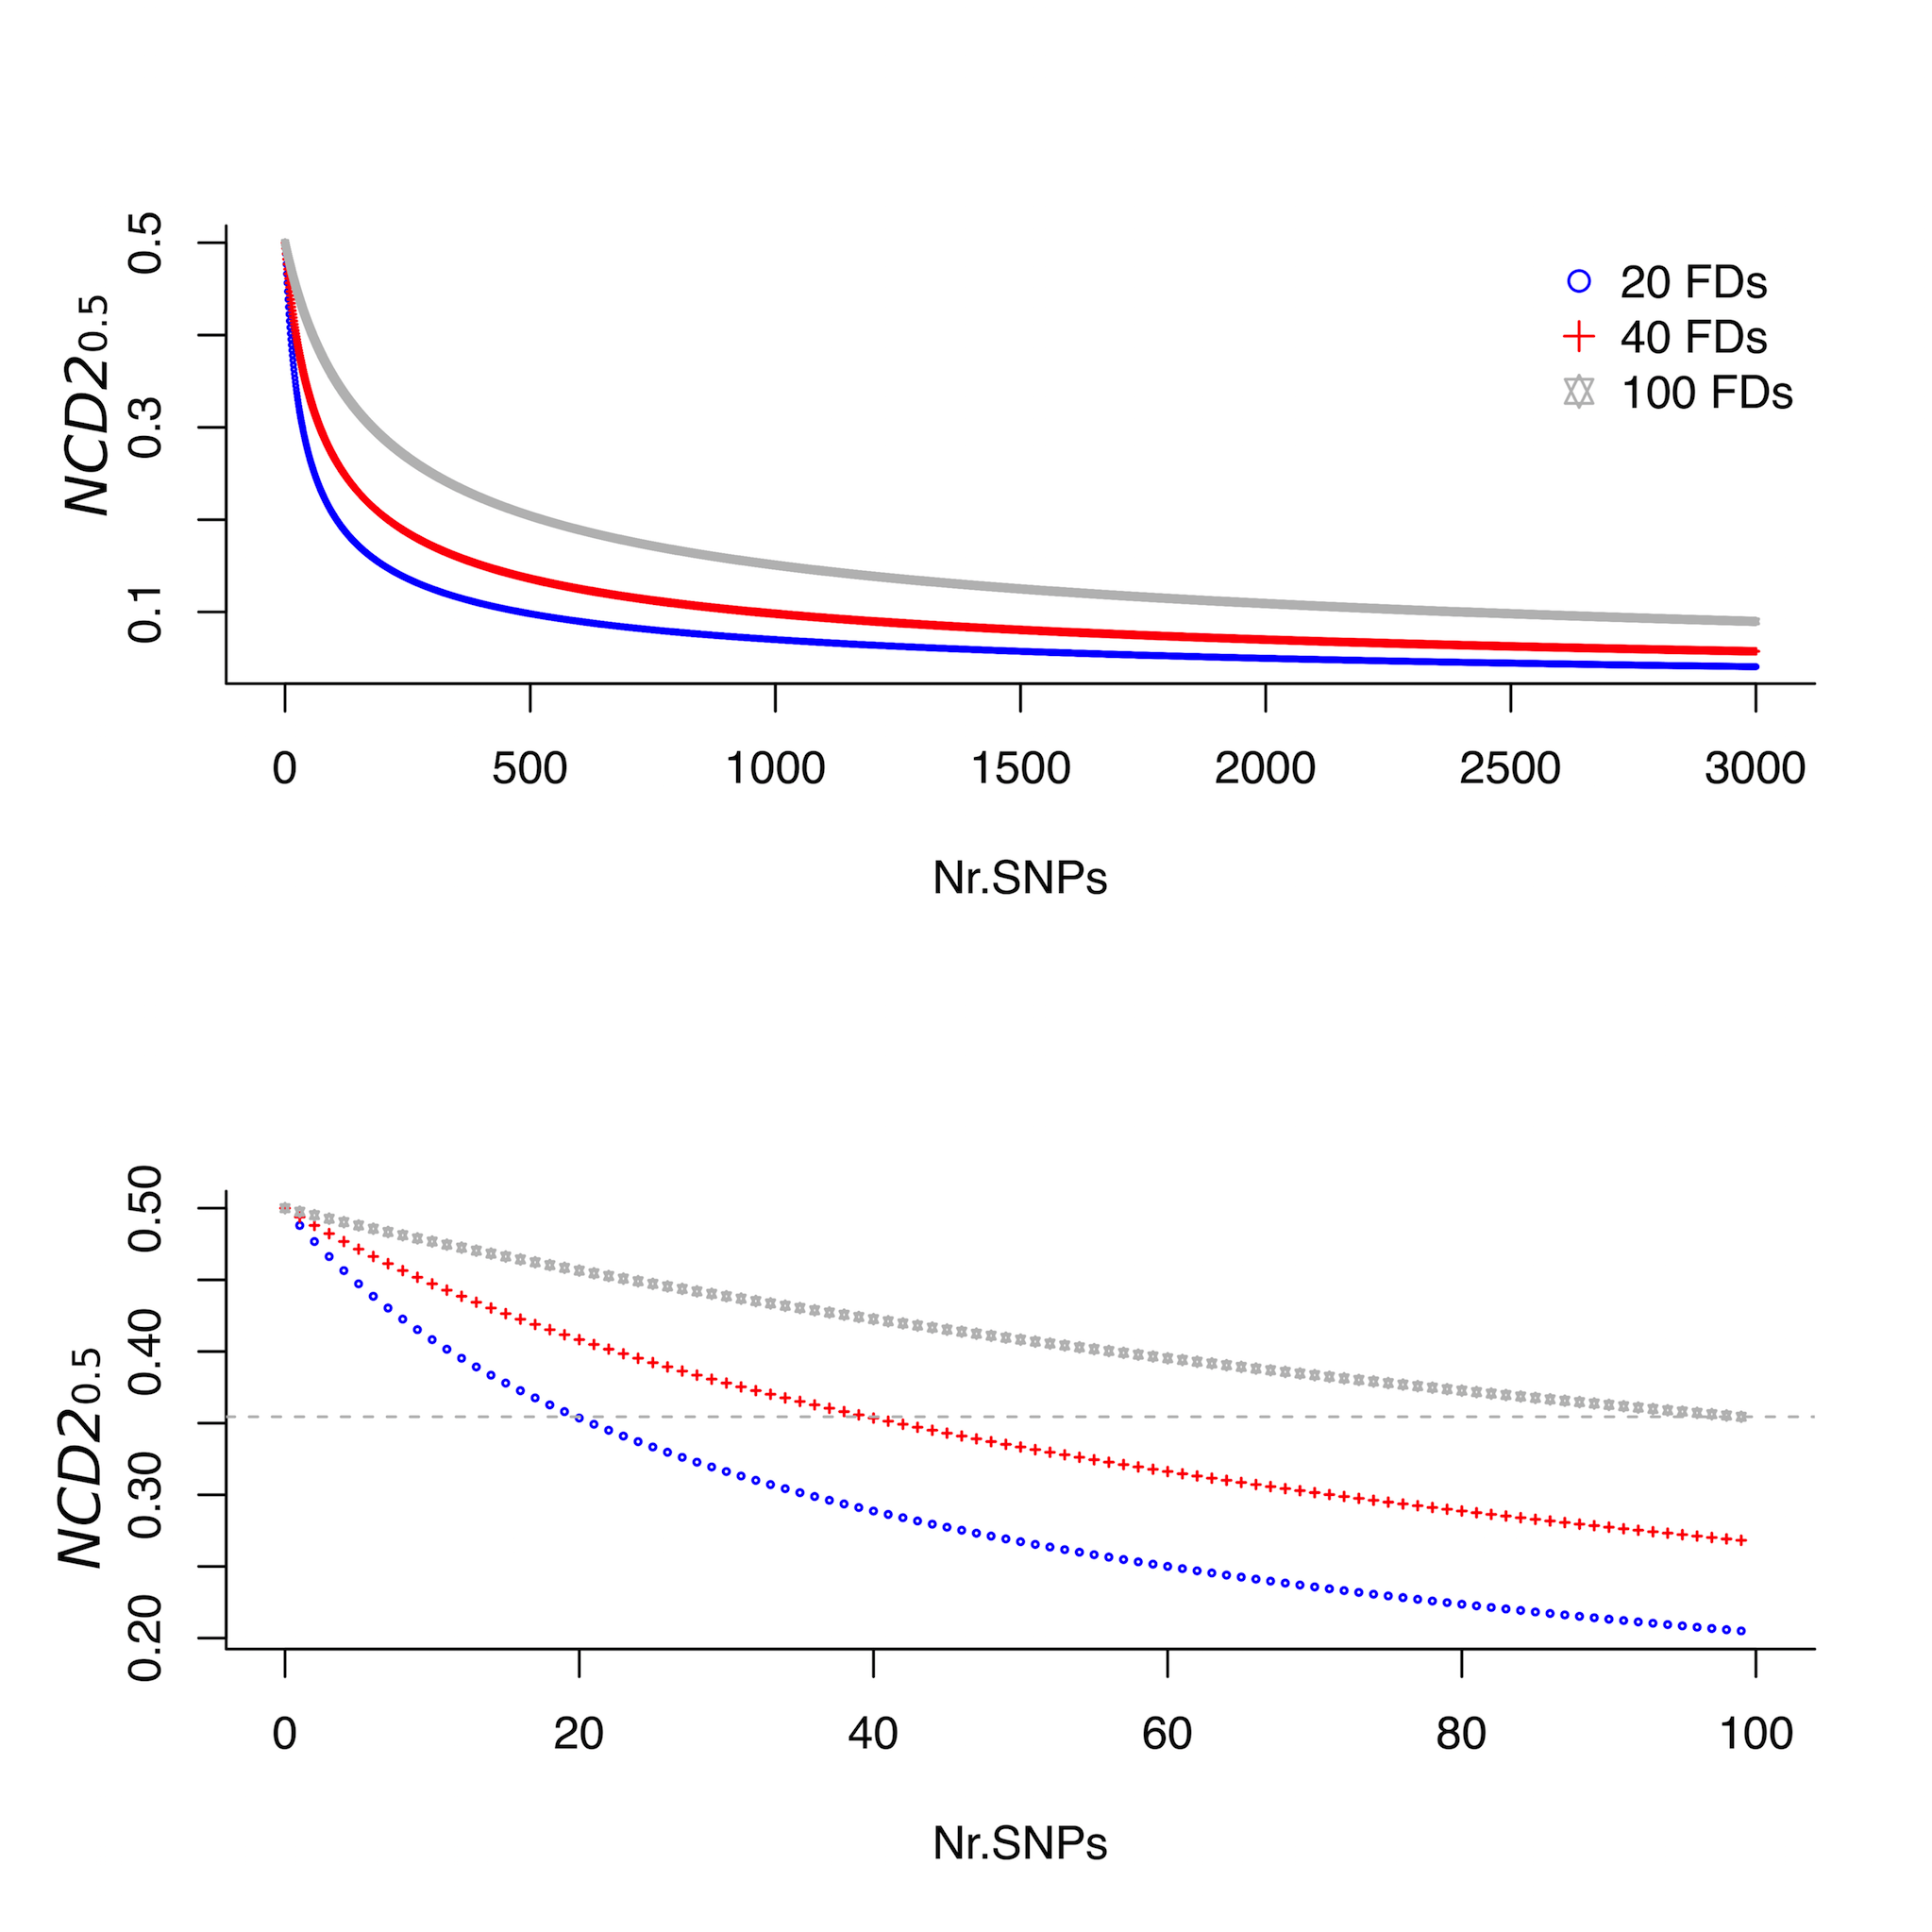
\includegraphics[width=0.8\textwidth, keepaspectratio]{chap2_folder/supp_figures/S1_Fig.png}
\caption*{\textbf{S1 Fig. NCD analytical properties as a function of number of SNPs}\\
x-axis, number of SNPs in the window for which $NCD2_{0.5}$ is being calculated; y-axis, $NCD2_{0.5}$ values. Each color corresponds to one (non-variable) number of FDs per window (20, 40, 100). Top, x-axis reaches 3,000 SNPs. After $\sim 1,500$ SNPs (for any of the number of FDs), $NCD2_{0.5}$ stabilizes and asymptotically approaches 0. Bottom, a zoom-in of the upper plot, with x-axis reaching only 100 SNPs. In this representation, all SNPs have a frequency of 0.5.}
\end{figure}
%
%
%

\begin{figure}[tbph]
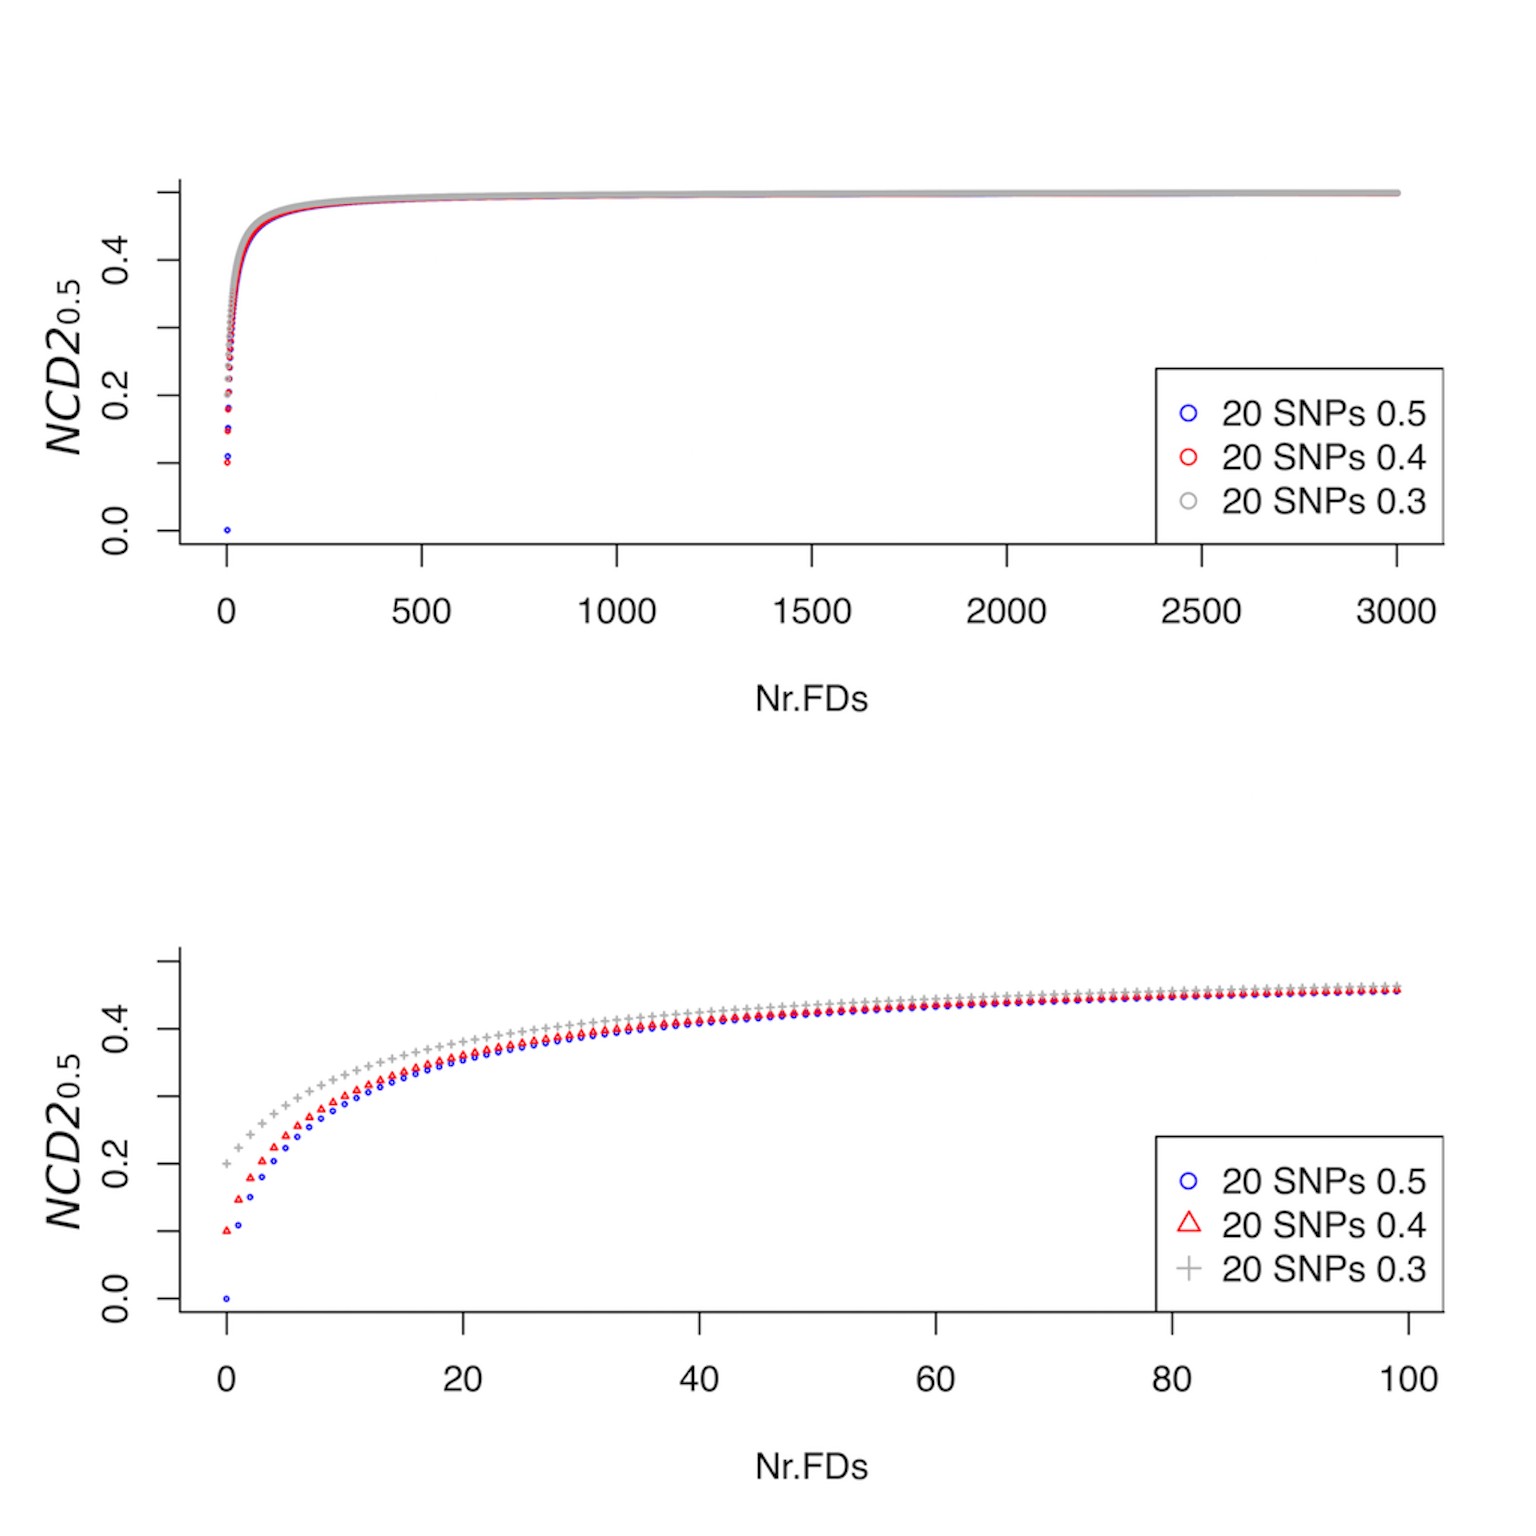
\includegraphics[]{chap2_folder/supp_figures/S2_Fig.png}
\caption*{\textbf{S2 Fig. Analytical properties of $NCD2$ as a function of number of FDs}\\
x-axis, number of FDs in the window for which $NCD2_{0.5}$ is being calculated; y-axis, $NCD2_{0.5}$ values. Each color corresponds to one the frequency of the 20 SNPs in the window (0.5, 0.4, 0.3). Top, x-axis reaches 3,000 FDs. After $\sim 500$ FDs, $NCD2_{0.5}$ stabilizes and asymptotically approaches 0.5; Bottom, a zoom-in of the upper plot, with x-axis reaching only 100 FDs. In this representation, all 20 SNPs have the same frequency (0.5 in blue, 0.4 in red, 0.3 in gray). Note that the minimum $NCD2_{0.5}$ value is different for the different colors, since they represent different SNP frequencies.}
\end{figure}
%
%

\begin{sidewaysfigure}[tbph]
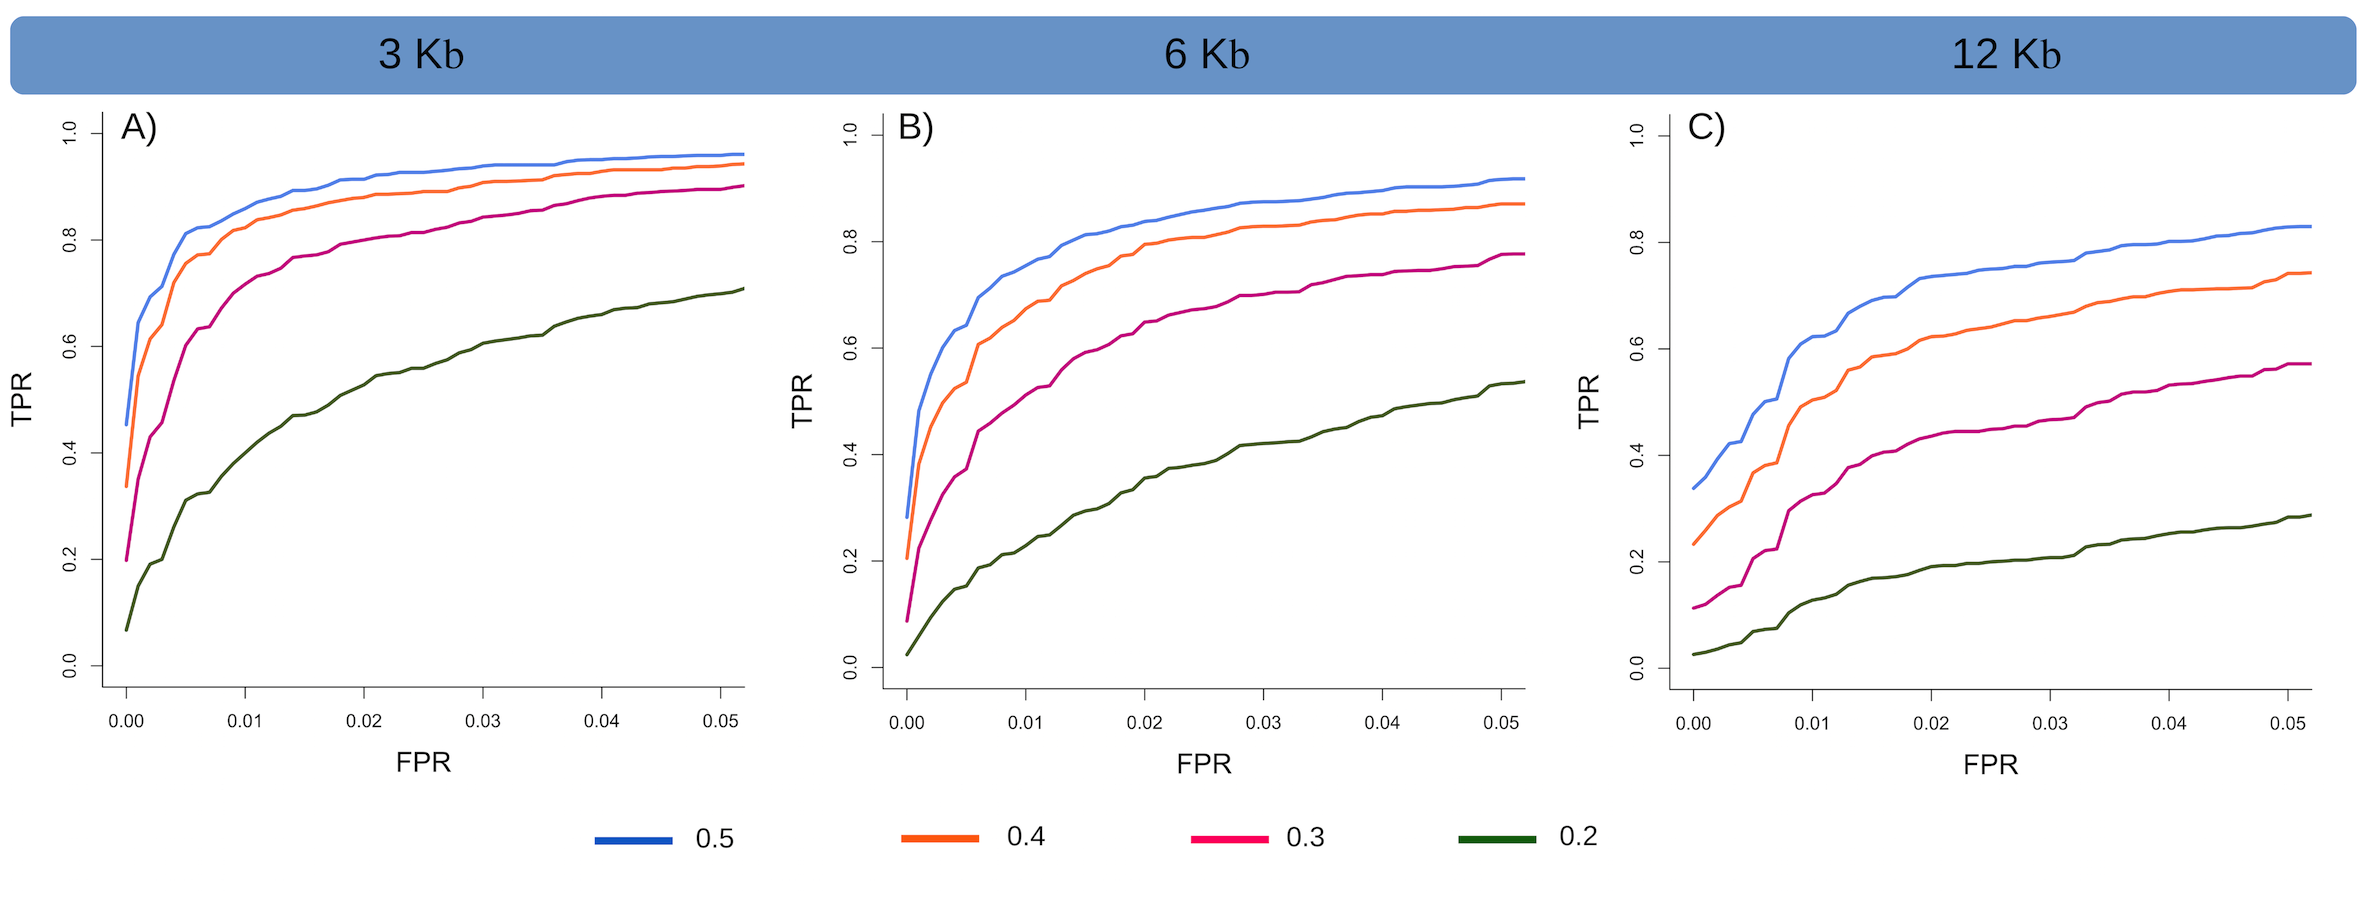
\includegraphics[]{chap2_folder/supp_figures/S3_Fig.png}
\caption*{\textbf{S3 Fig.Effect of sequence length on $NCD2_{0.5}$ power (Africa). }\\
ROC curves for sequence lengths (\emph{L}) of (A) 3 Kb, (B) 6 Kb, and (C) 12 Kb. Each plot shows $NCD2_{0.5}$ performance for simulations where the balanced polymorphism is modeled to achieve an equilibrium frequency ($f_{\mathrm{eq}}$) of 0.5 (blue), 0.4 (orange), 0.3 (pink), or 0.2 (green), based on simulations under the African demographic scenario and $Tbs = 5$ myr. FPR, false positive rate (100-Specificity); TPR, true positive rate (sensitivity, or power). Note that the x-axis ranges from 0 to 0.05, while the y-axis ranges from 0 to 1.}
\end{sidewaysfigure}

%
%
\begin{sidewaysfigure}[tbph]
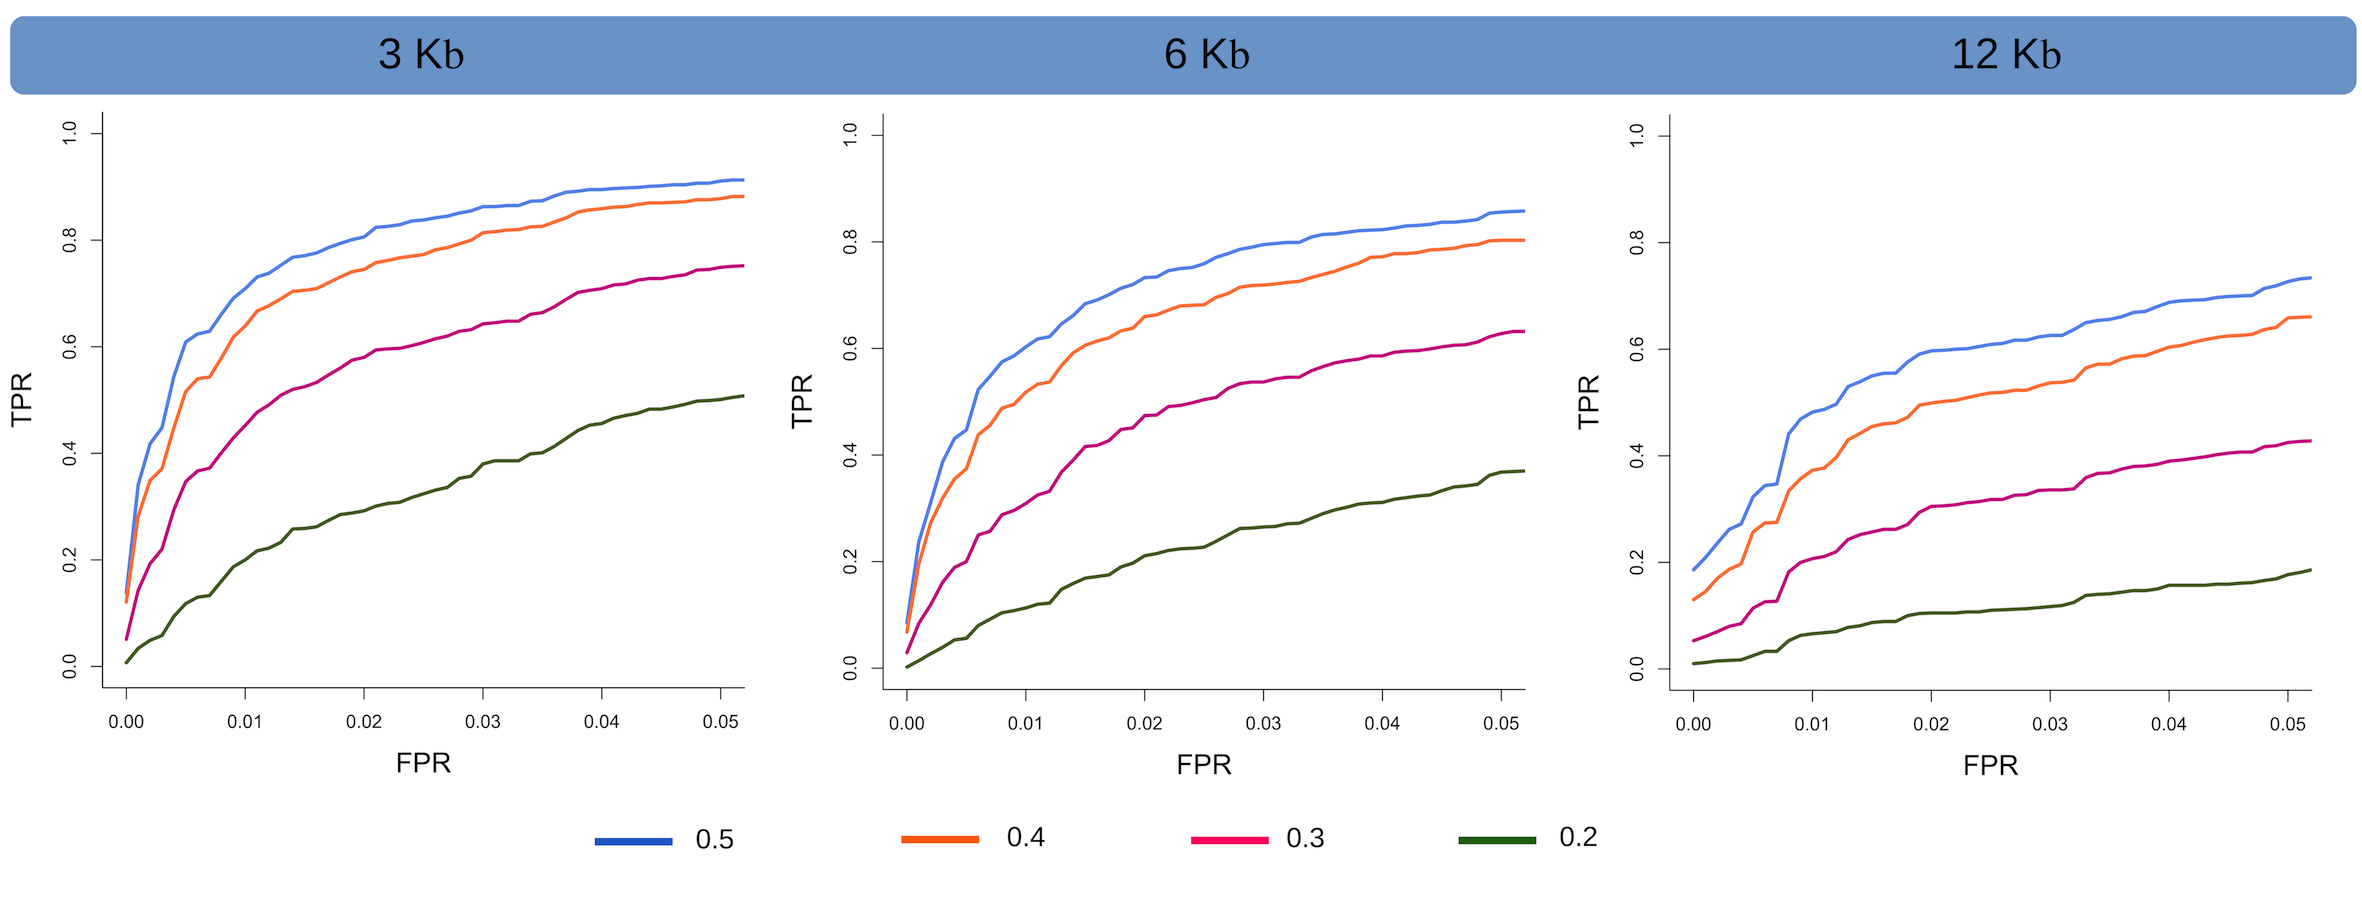
\includegraphics[]{chap2_folder/supp_figures/S4_Fig.png}
\caption*{\textbf{S4 Fig.Effect of sequence length on $NCD2_{0.5}$ power (Africa). }\\
ROC curves for sequence lengths (\emph{L}) of (A) 3Kb, (B) 6Kb, and (C) 12 Kb. Each plot shows $NCD2_{0.5}$ performance for simulations where the balanced polymorphism is modeled to achieve an equilibrium frequency ($f_{\mathrm{eq}}$) of 0.5 (blue), 0.4 (orange), 0.3 (pink), or 0.2 (green), based on simulations under the African demographic scenario and $Tbs = 3$ myr. FPR, false positive rate (100-Specificity); TPR, true positive rate (sensitivity, or power). Note that the x-axis ranges from 0 to 0.05, while the y-axis ranges from 0 to 1.}
\end{sidewaysfigure}
%
%

\begin{sidewaysfigure}[tbph]
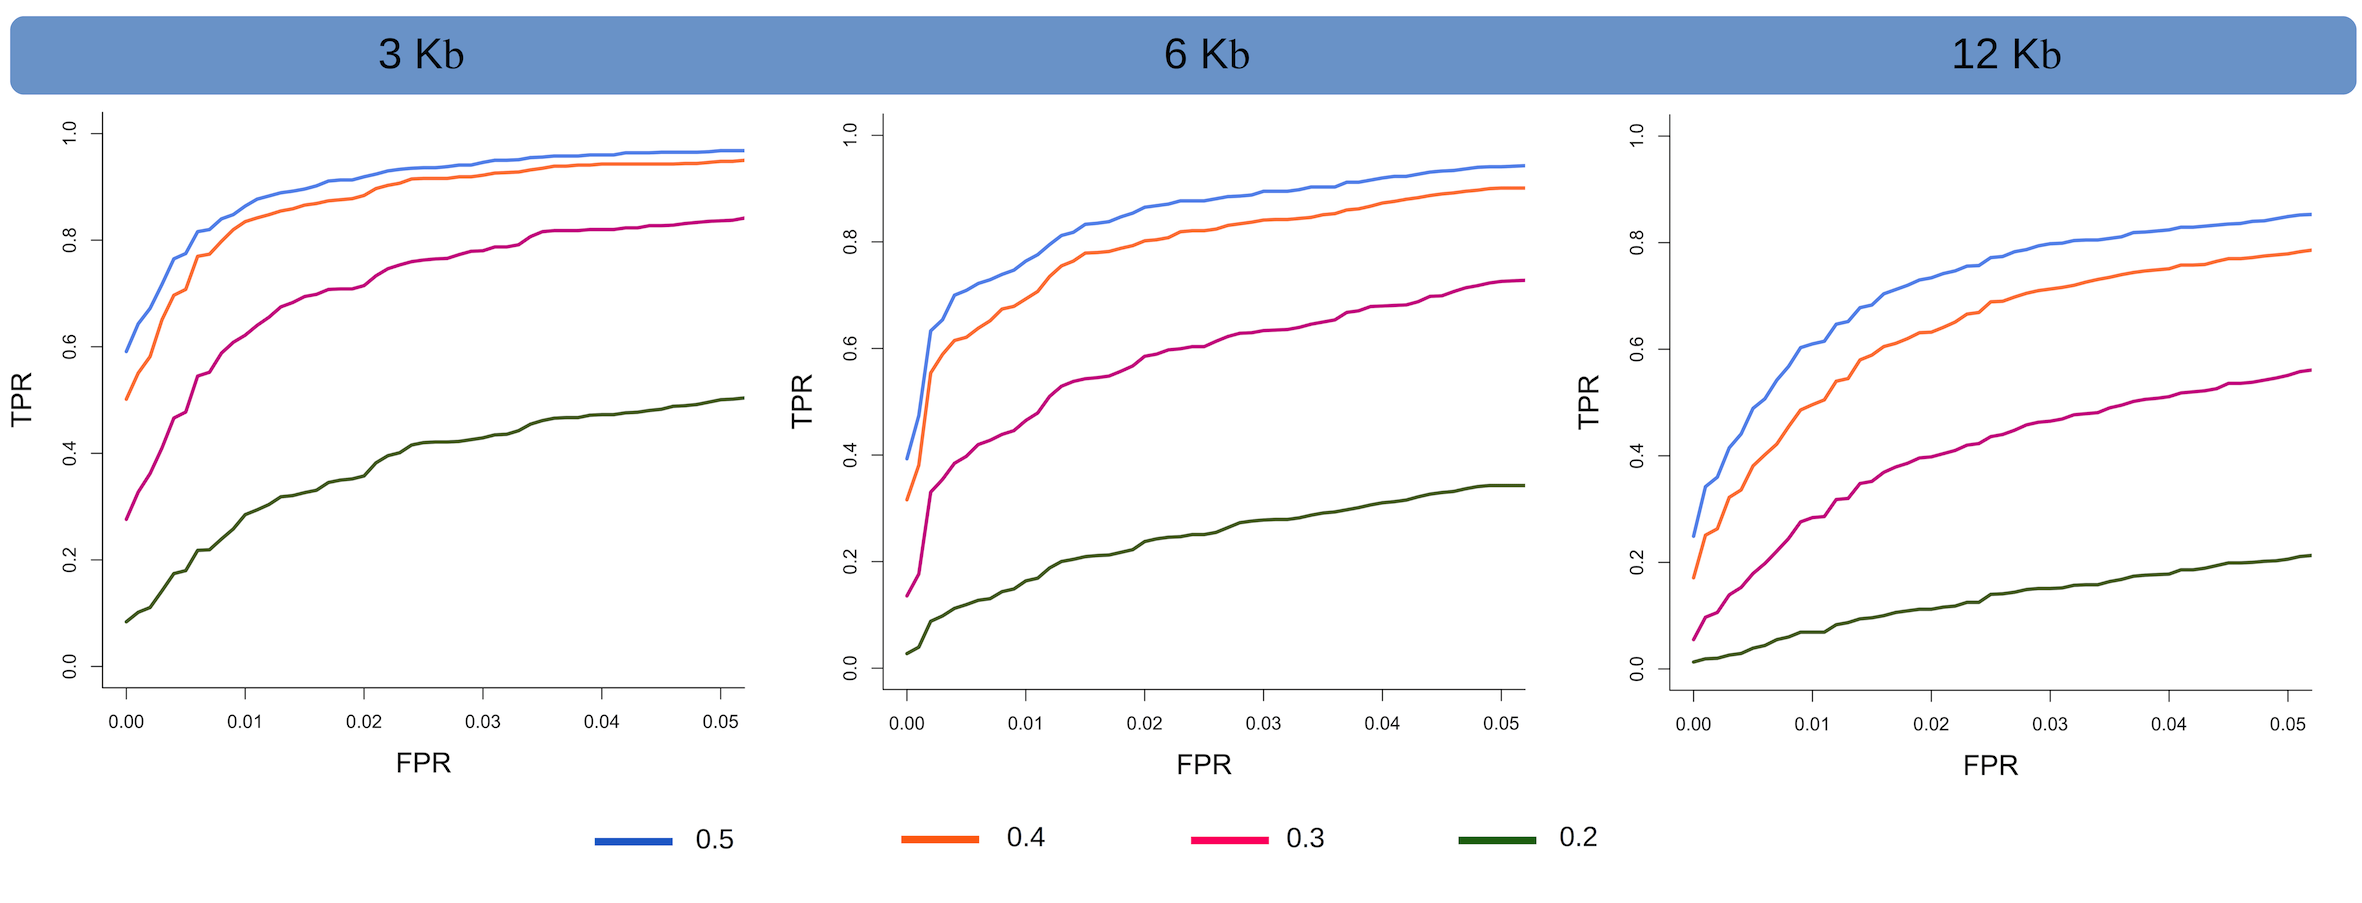
\includegraphics[]{chap2_folder/supp_figures/S5_Fig.png}
\caption*{\textbf{S5 Fig.Effect of sequence length on $NCD2_{0.5}$ power (Europe). }\\
ROC curves for sequence lengths (\emph{L}) of (A) 3Kb, (B) 6Kb, and (C) 12 Kb. Each plot shows $NCD2_{0.5}$ performance for simulations where the balanced polymorphism is modeled to achieve an equilibrium frequency ($f_{\mathrm{eq}}$) of 0.5 (blue), 0.4 (orange), 0.3 (pink), or 0.2 (green), based on simulations under the European demographic scenario and $Tbs = 5$ myr. FPR, false positive rate (100-Specificity); TPR, true positive rate (sensitivity, or power). Note that the x-axis ranges from 0 to 0.05, while the y-axis ranges from 0 to 1.}
\end{sidewaysfigure}
%
%
\begin{sidewaysfigure}[tbph]
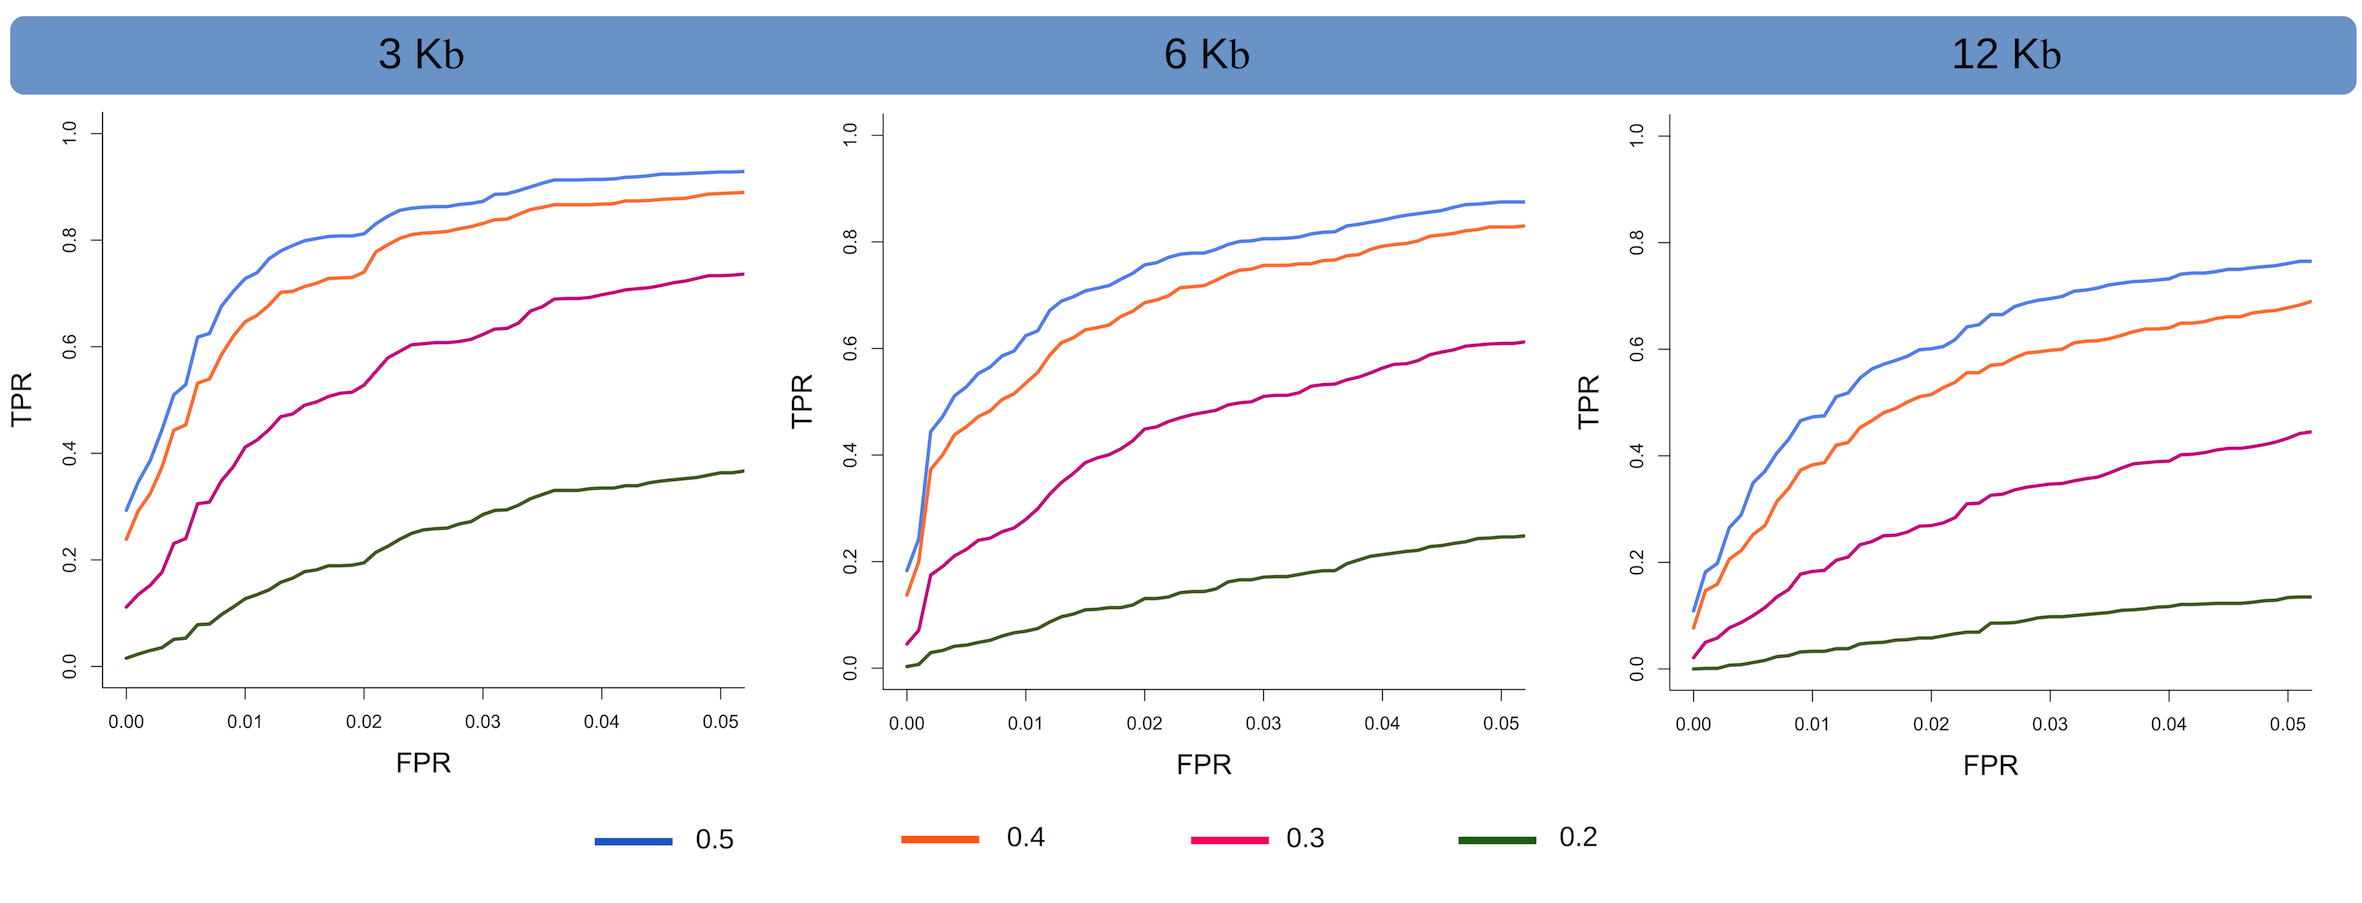
\includegraphics[]{chap2_folder/supp_figures/S6_Fig.png}
\caption*{\textbf{S6 Fig.Effect of sequence length on $NCD2_{0.5}$ power (Europe). }\\
ROC curves for sequence lengths (\emph{L}) of (A) 3Kb, (B) 6Kb, and (C) 12 Kb. Each plot shows $NCD2_{0.5}$ performance for simulations where the balanced polymorphism is modeled to achieve an equilibrium frequency ($f_{\mathrm{eq}}$) of 0.5 (blue), 0.4 (orange), 0.3 (pink), or 0.2 (green), based on simulations under the European demographic scenario and $Tbs = 3$ myr. FPR, false positive rate (100-Specificity); TPR, true positive rate (sensitivity, or power). Note that the x-axis ranges from 0 to 0.05, while the y-axis ranges from 0 to 1.}
\end{sidewaysfigure}
%
%

\begin{sidewaysfigure}[tbph]
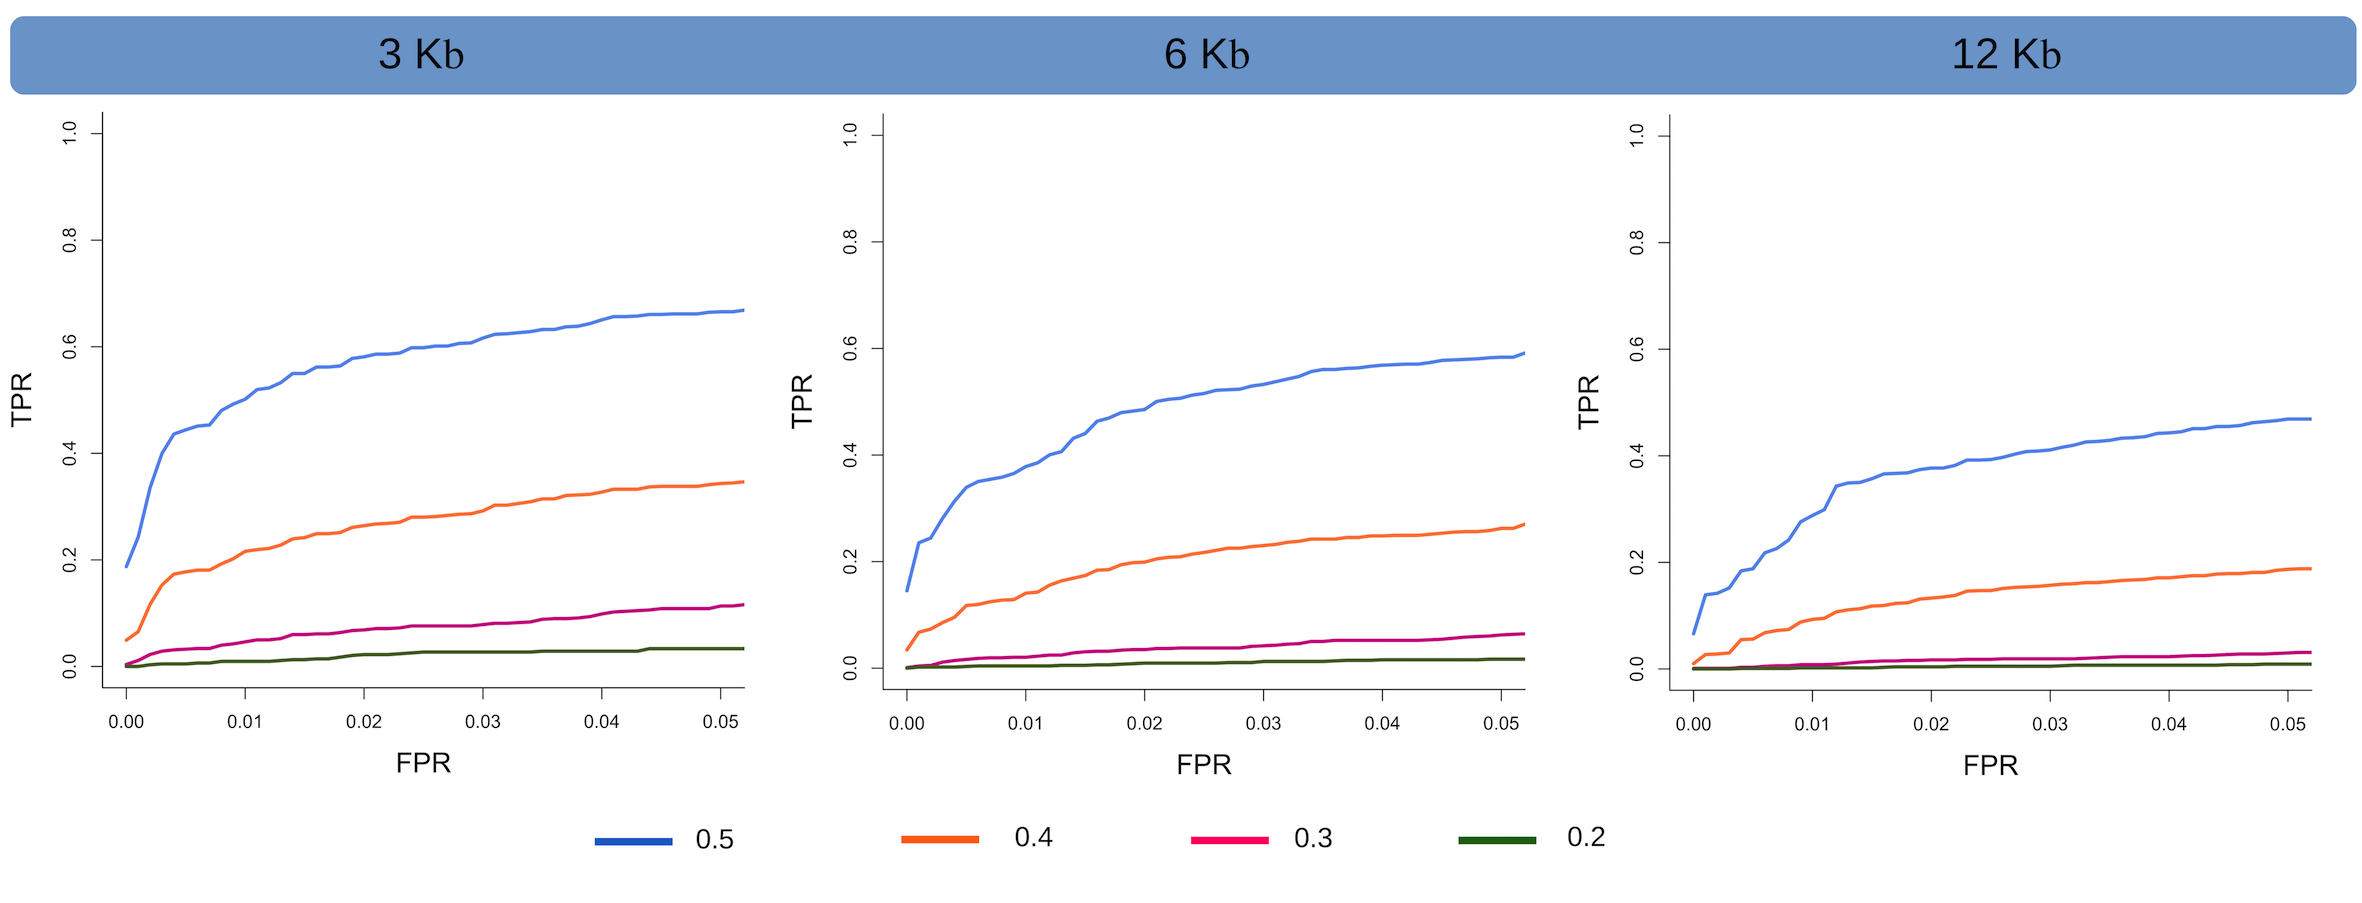
\includegraphics[]{chap2_folder/supp_figures/S7_Fig.png}
\caption*{\textbf{S7 Fig.Effect of sequence length on $NCD2_{0.5}$ power (Asia). }\\
ROC curves for sequence lengths (\emph{L}) of (A) 3Kb, (B) 6Kb, and (C) 12 Kb. Each plot shows $NCD2_{0.5}$ performance for simulations where the balanced polymorphism is modeled to achieve an equilibrium frequency ($f_{\mathrm{eq}}$) of 0.5 (blue), 0.4 (orange), 0.3 (pink), or 0.2 (green), based on simulations under the Asian demographic scenario and $Tbs = 5$ myr. FPR, false positive rate (100-Specificity); TPR, true positive rate (sensitivity, or power). Note that the x-axis ranges from 0 to 0.05, while the y-axis ranges from 0 to 1.}
\end{sidewaysfigure}
%
\begin{sidewaysfigure}[tbph]
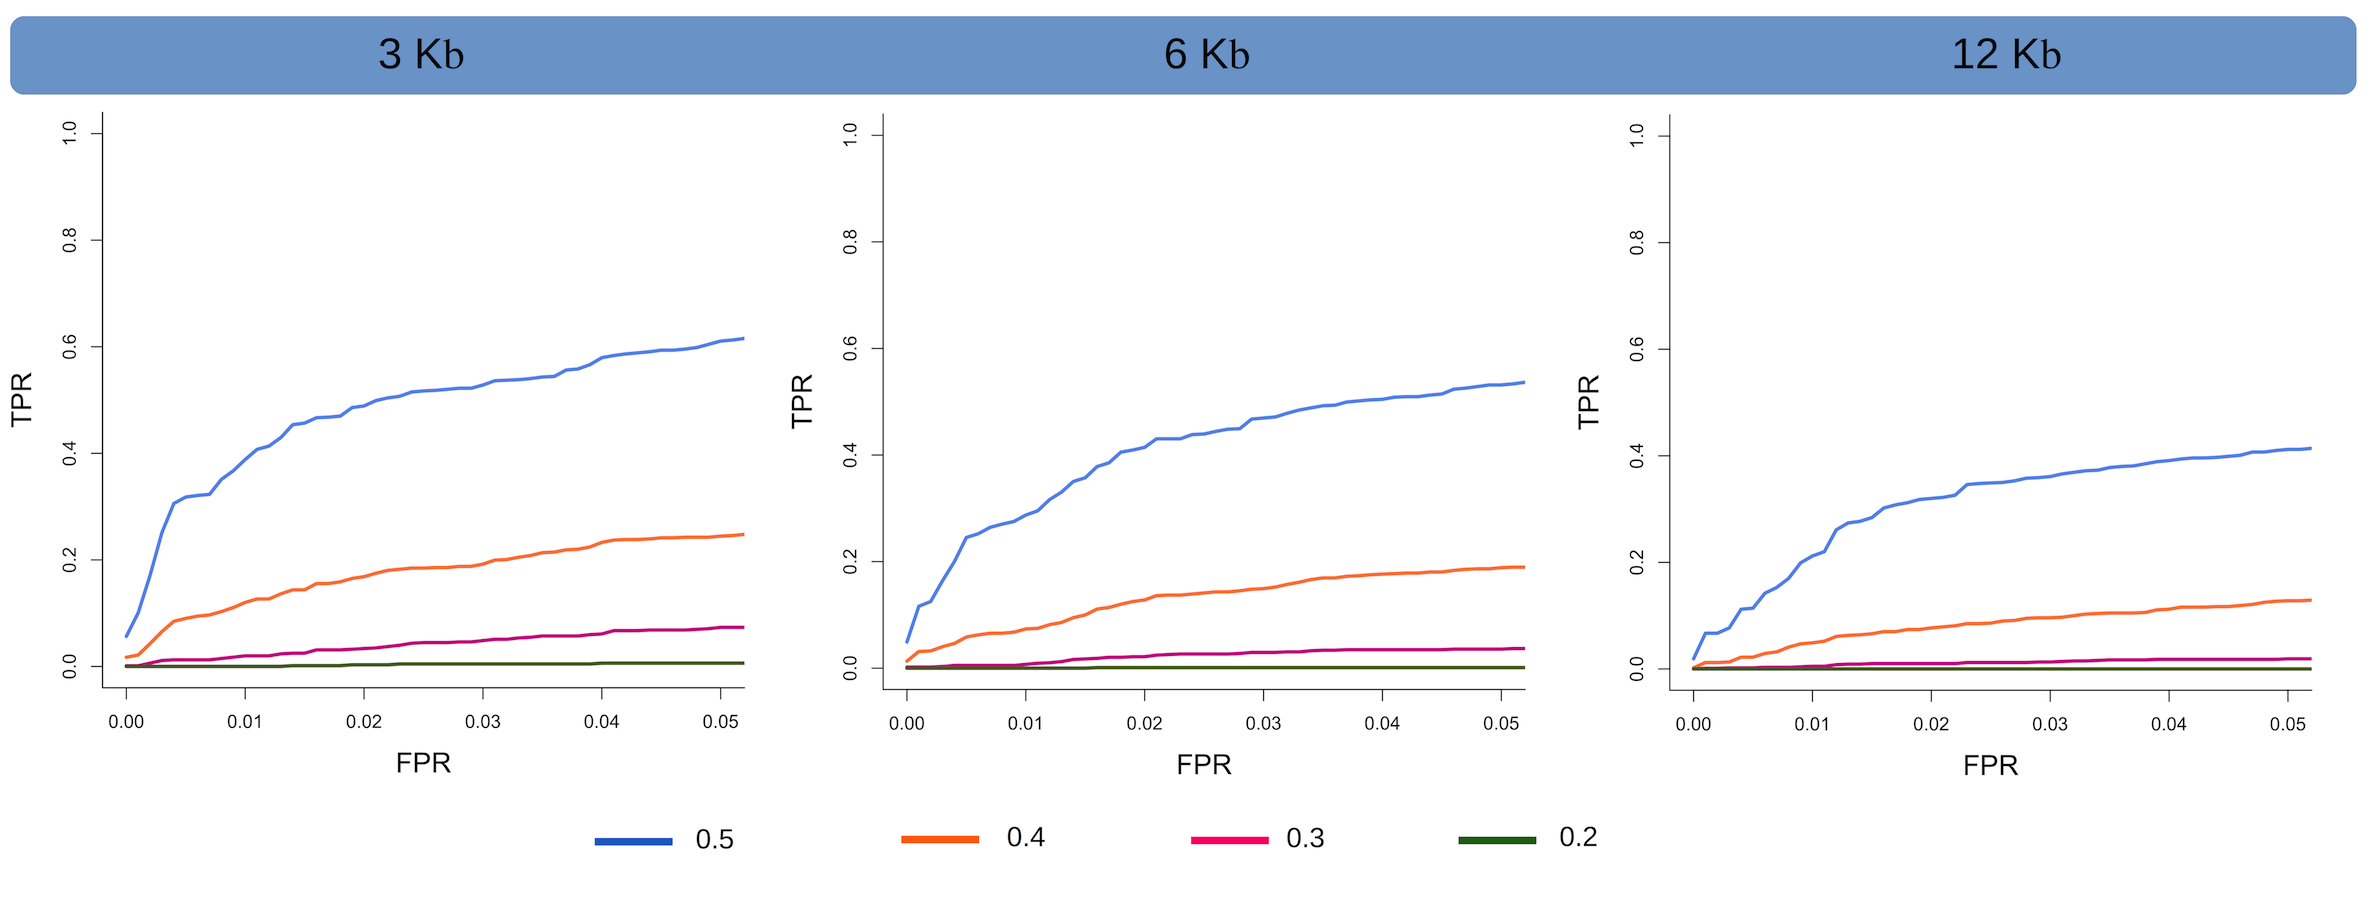
\includegraphics[]{chap2_folder/supp_figures/S8_Fig.png}
\caption*{\textbf{S8 Fig.Effect of sequence length on $NCD2_{0.5}$ power (Asia). }\\
ROC curves for sequence lengths (\emph{L}) of (A) 3Kb, (B) 6Kb, and (C) 12 Kb. Each plot shows $NCD2_{0.5}$ performance for simulations where the balanced polymorphism is modeled to achieve an equilibrium frequency ($f_{\mathrm{eq}}$) of 0.5 (blue), 0.4 (orange), 0.3 (pink), or 0.2 (green), based on simulations under the Asian demographic scenario and $Tbs = 3$ myr. FPR, false positive rate (100-Specificity); TPR, true positive rate (sensitivity, or power). Note that the x-axis ranges from 0 to 0.05, while the y-axis ranges from 0 to 1.}
\end{sidewaysfigure}
%
\begin{figure}[tbph]
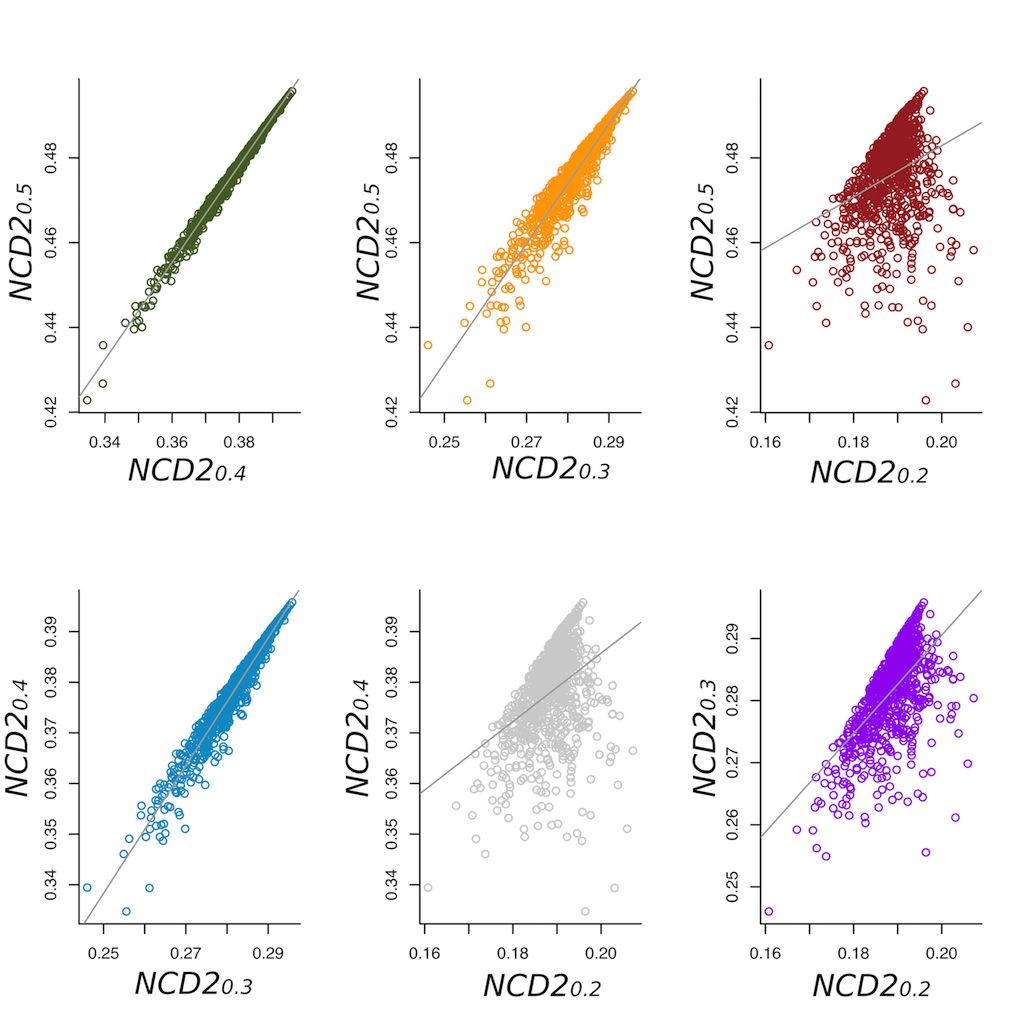
\includegraphics[]{chap2_folder/supp_figures/S9_Fig.png}
\caption*{\textbf{Fig S9. Correlations for $NCD2_{\mathrm{tf}}$ calculated with different $tf$ values.}\\
In each plot, $NCD2$ values calculated with two different target frequencies are plotted against each other. $NCD2$ was calculated for 1,000 neutral simulations following demographic parameters for the African continent. $L= 3$ Kb.
}
\end{figure}
%
\begin{sidewaysfigure}[tbph]
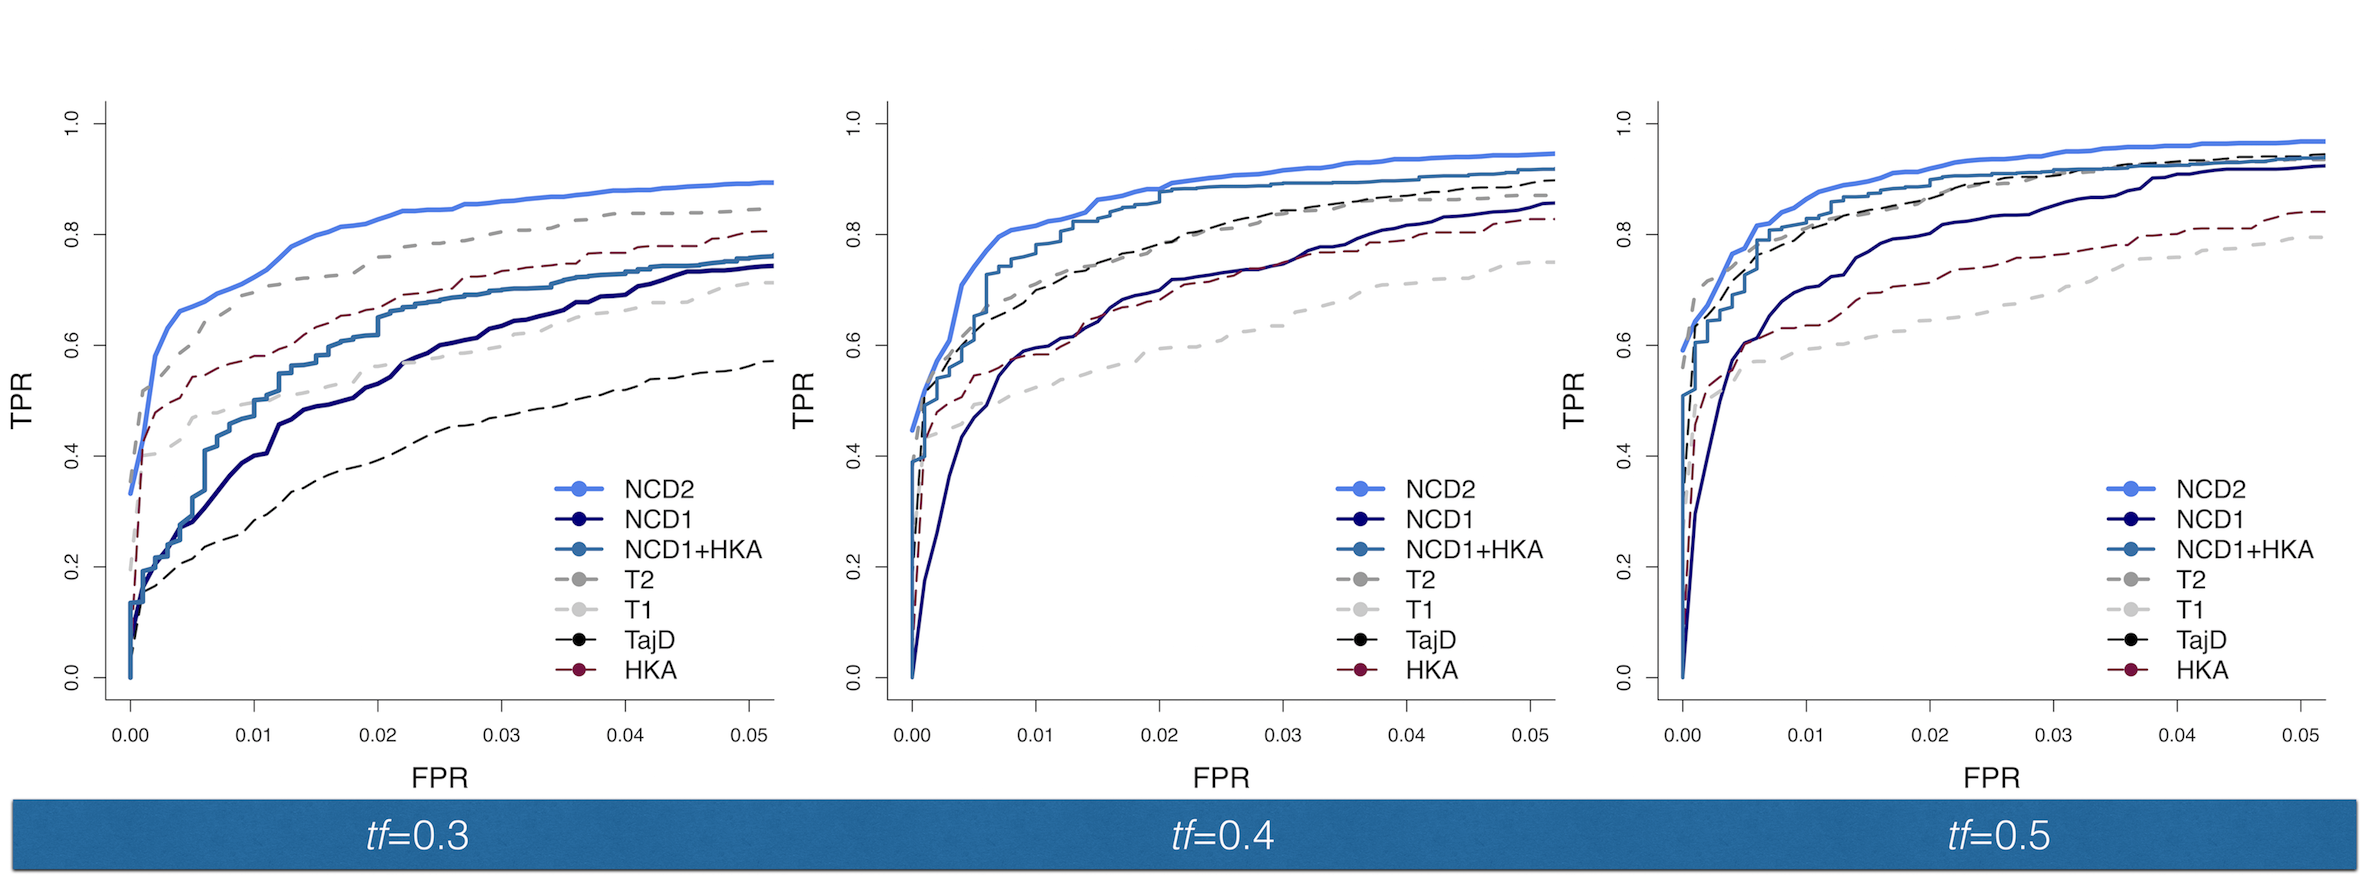
\includegraphics[]{chap2_folder/supp_figures/S10.png}
\caption*{\textbf{Fig S10. ROC curves for comparison between NCD20.5 and other tests (Europe). }\\
Power to detect LTBS for simulations where the balanced polymorphism was modeled to achieve frequency equilibrium ($f_{\mathrm{eq}}$) of (left) 0.3, (center) 0.4, and (right) 0.5. Plotted values are for European demography, $Tbs = 5$ myr, $L = 3$ kb). Target frequency for $NCD1$ and $NCD2$ matches the simulated $f_{\mathrm{eq}}$. 
}
\end{sidewaysfigure}

%% FIGURE %%% FIGURE %%% FIGURE %%% FIGURE %%% FIGURE %%% FIGURE %%% FIGURE %%% FIGURE %%% FIGURE %%% FIGURE %%% FIGURE %%% FIGURE %%% FIGURE %%
\begin{figure}[h]
\centering
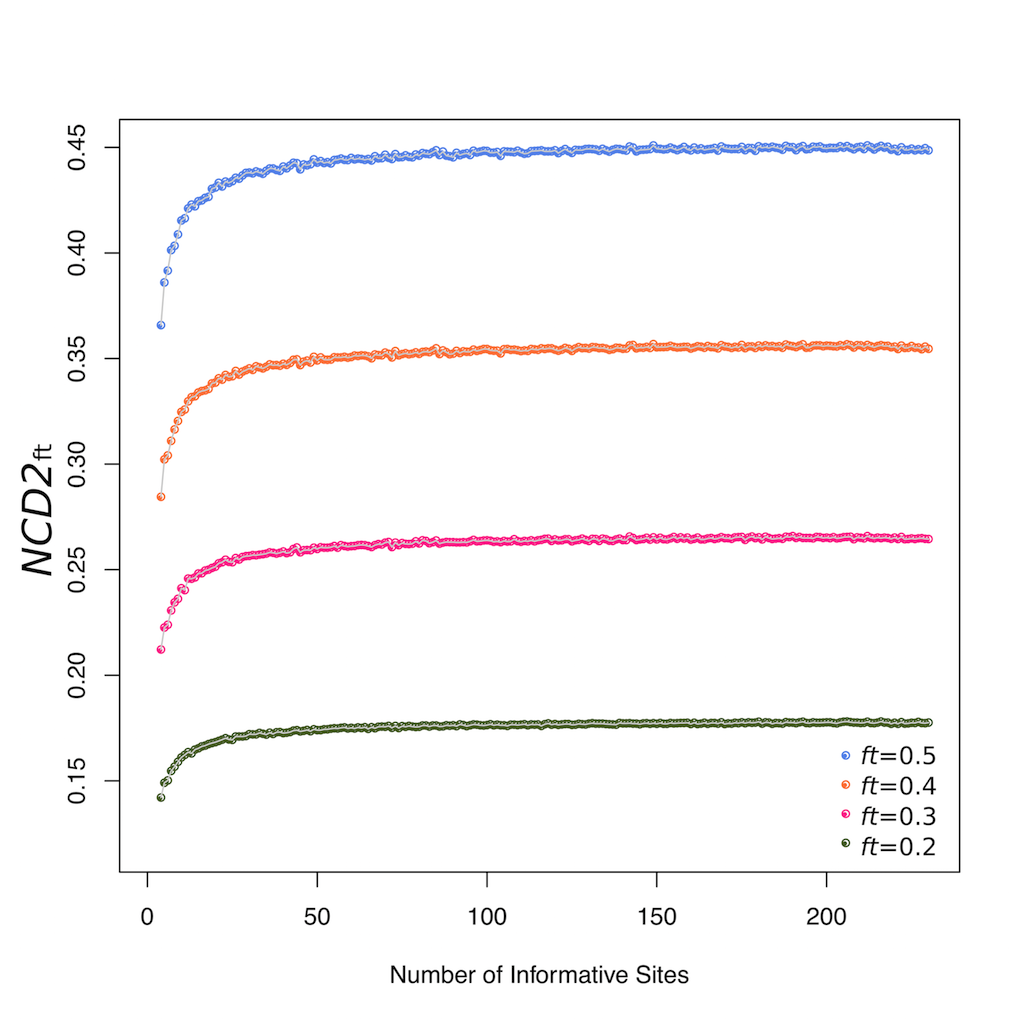
\includegraphics[width=0.9\textwidth, keepaspectratio]{chap2_folder/supp_figures/S11_Fig.png}
\caption*{\textbf{Fig S11. Relationship between NDC2tf and the number of informative sites.}\\
$NCD2_{\mathrm{tf}}$ was calculated for neutral simulations (10,000 for each bin of IS) for African demographic scenario and the 0.01 quantile value for each bin is plotted. Blue ($tf=0.5$), orange ($tf=0.4$), pink ($tf=0.3$), green ($tf=0.2$).
}
\end{figure}
%
\begin{figure}[h]
\centering
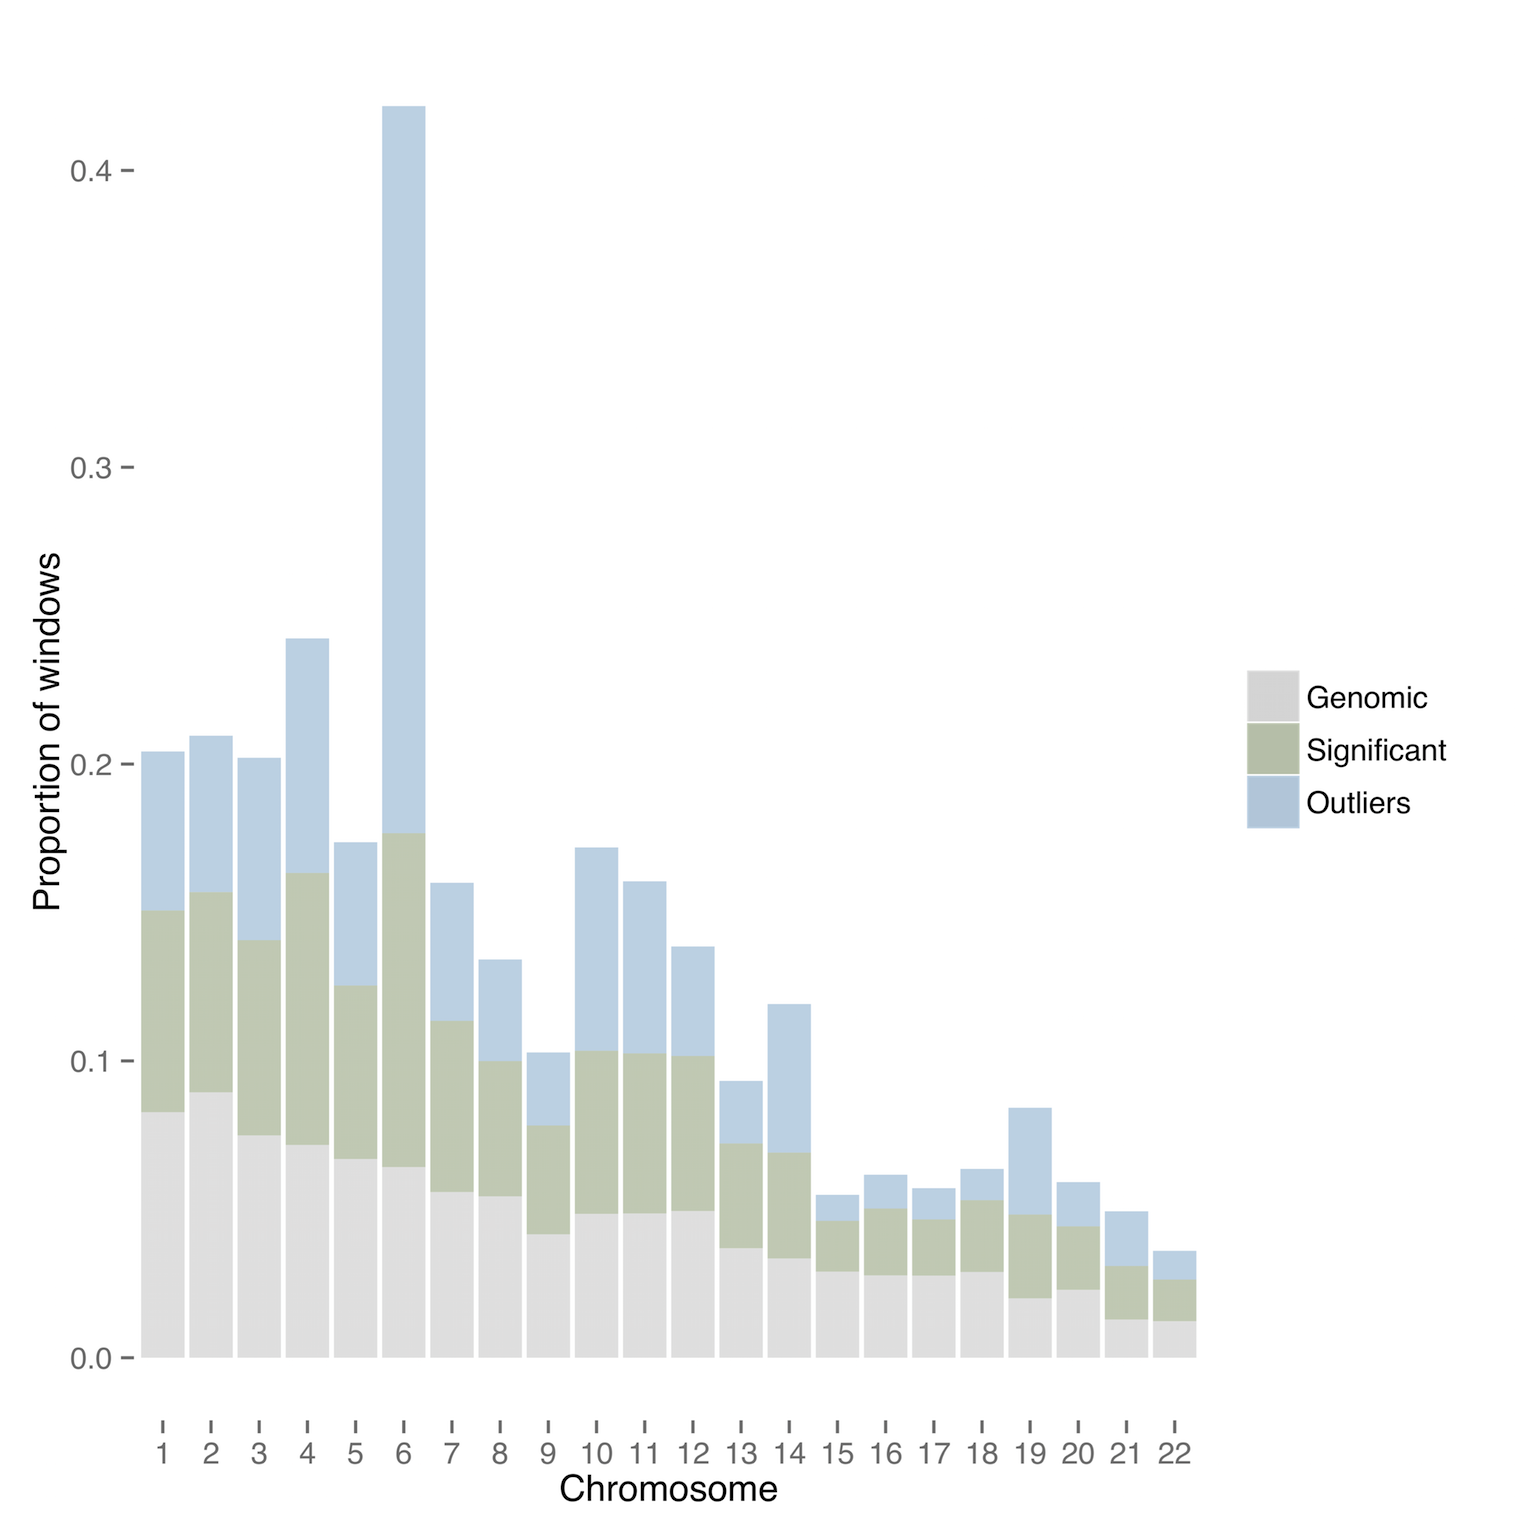
\includegraphics[width=0.65\textwidth, keepaspectratio]{chap2_folder/supp_figures/S12_Fig.png}
\caption*{\textbf{Fig S12. Proportion of windows per chromosome.}  Sets of significant and outlier windows are derived from the union of three target frequencies (0.3, 0.4, 0.5). Grey, all genomic windows; significant (green) and (blue) outlier windows. 
}
\end{figure}
%
\begin{figure}[h]
\centering
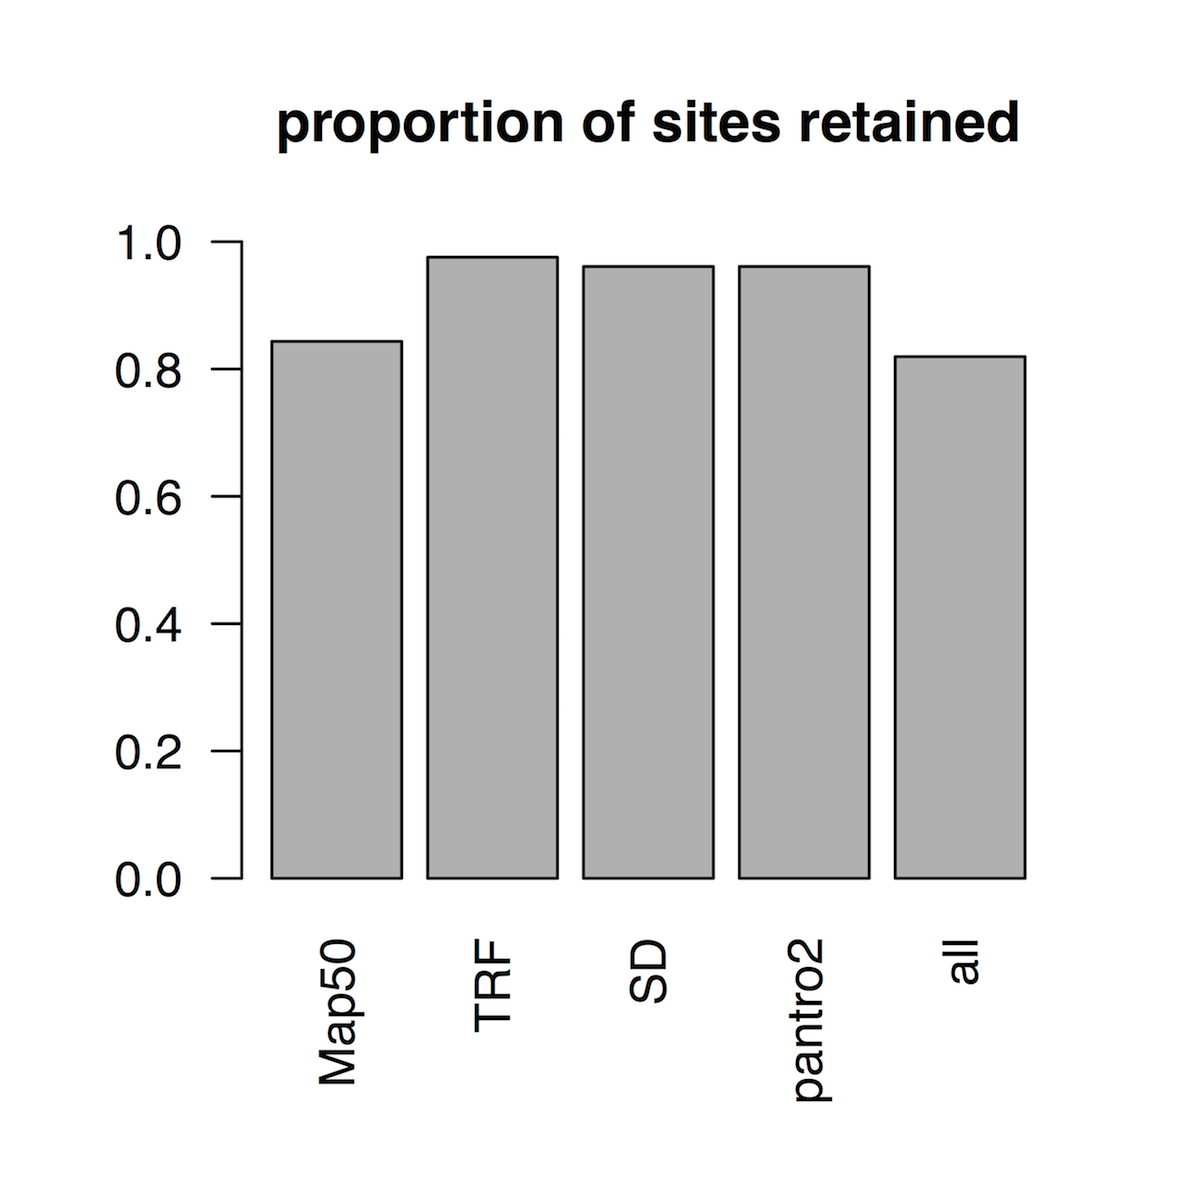
\includegraphics[width=0.3\textwidth,keepaspectratio]{chap2_folder/supp_figures/S13_fig.png}
\caption*{\textbf{Fig S13. Proportion of positions in the genome retained after each filter.}
Proportion of the hg19 human reference genome (total base-pairs = 2,684,573,005) retained for each individual filtering criterium described in the Methods, and for all filters jointly applied together. Proportion of sequences retained: Map50=0.843; TRF=0.976; SD=0.961; pantro2=0.961; all=0.819. Map50: mappability 50-mer (see Methods); TRF: tandem repeats; SD: segmental duplications; pantro2: reference chimp genome. 
}
\end{figure}
%

\begin{figure}[]
\centering
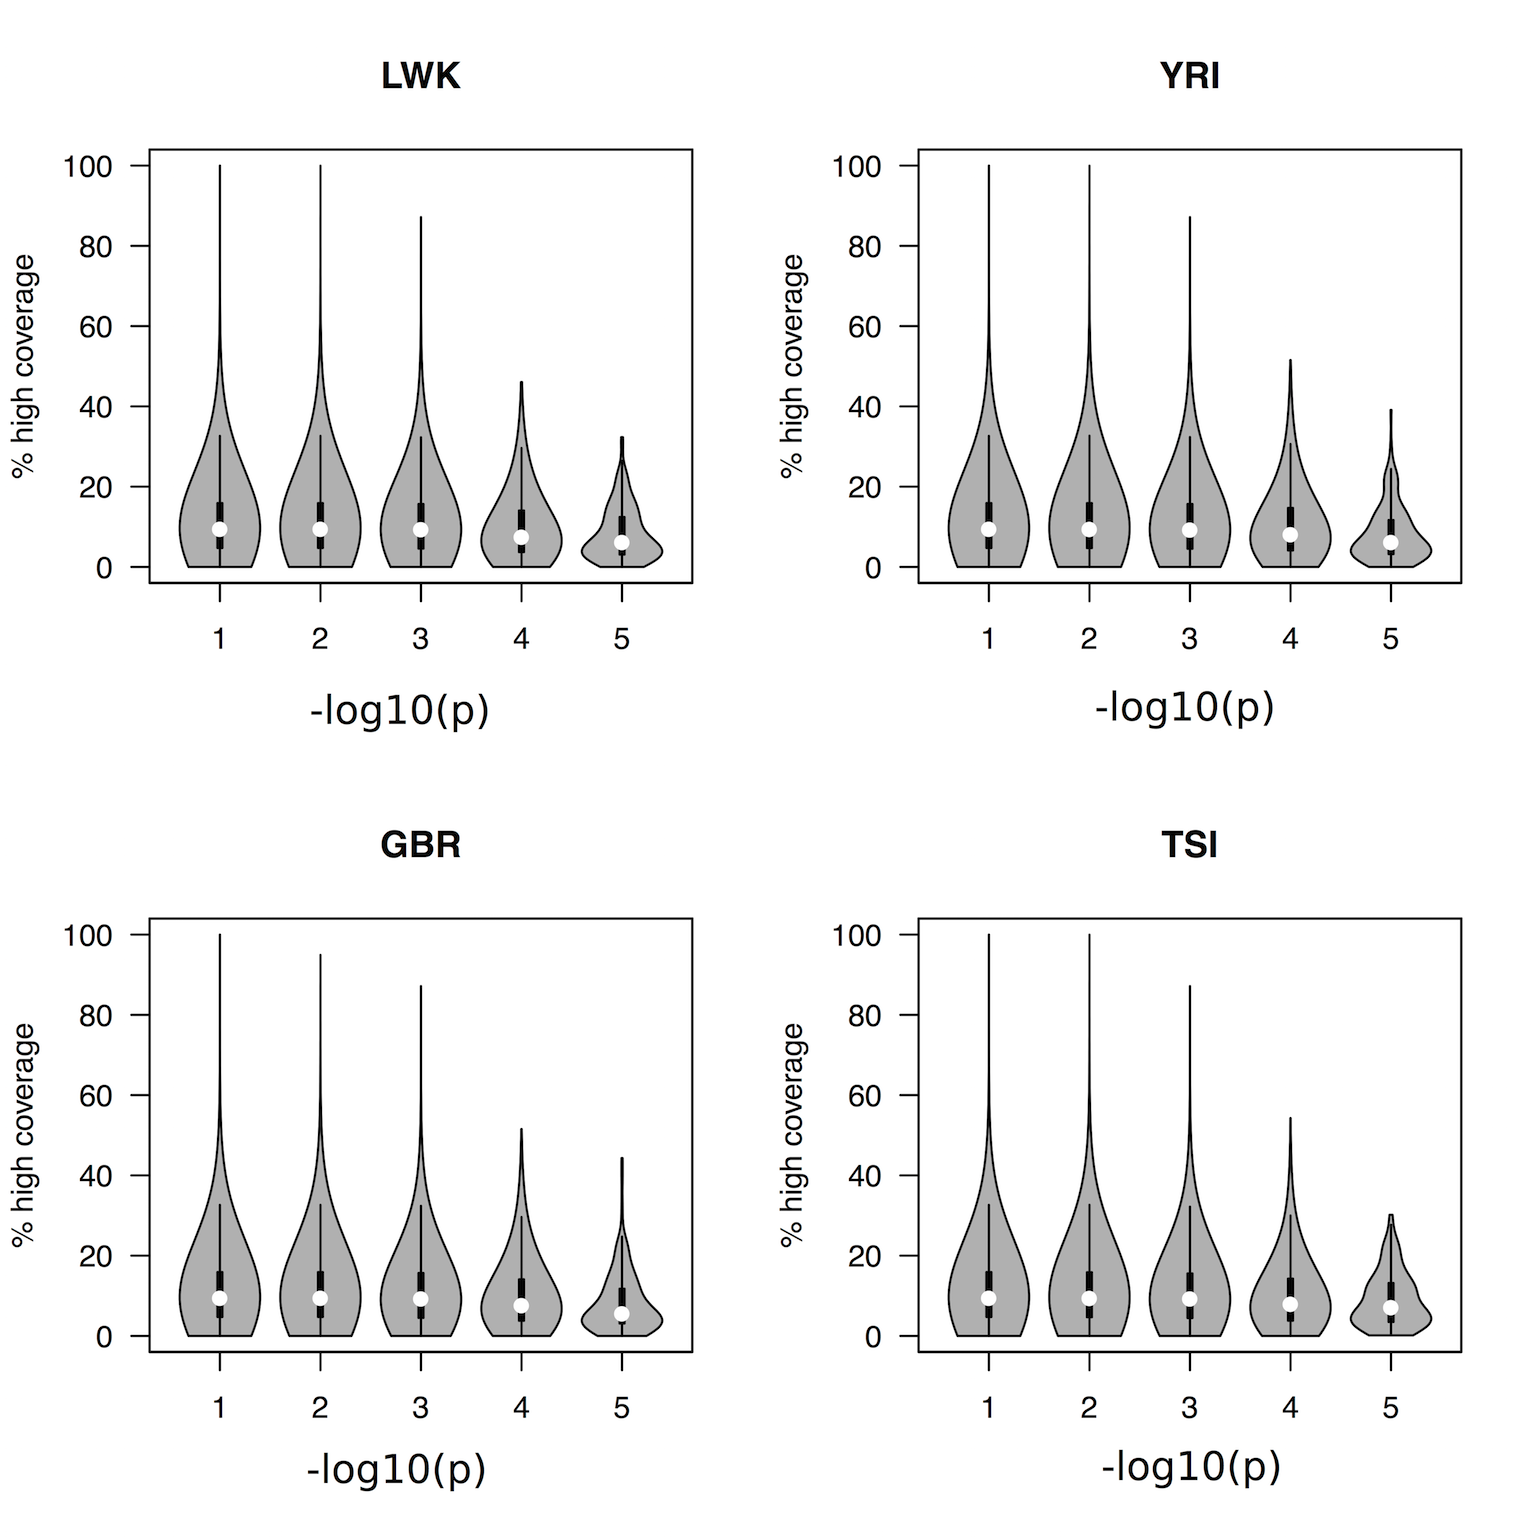
\includegraphics[]{chap2_folder/supp_figures/S14_Fig.png}
\caption*{\textbf{Fig S14. Distribution of proportion of high coverage (pHC) positions per bin of empirical $NCD2$ \emph{p}-value.}  
pHC in percentage (y-axis) binned by the $NCD2$ $Z_{\mathrm{tf}}$ empirical \emph{p}-values represented in –log10 scale on the x-axis. pHC is the proportion of the sequence of a given window in this study having high coverage values in at least two samples of modern human shotgun data (see Methods). 
}
\end{figure}
%
\begin{figure}[h]
\centering
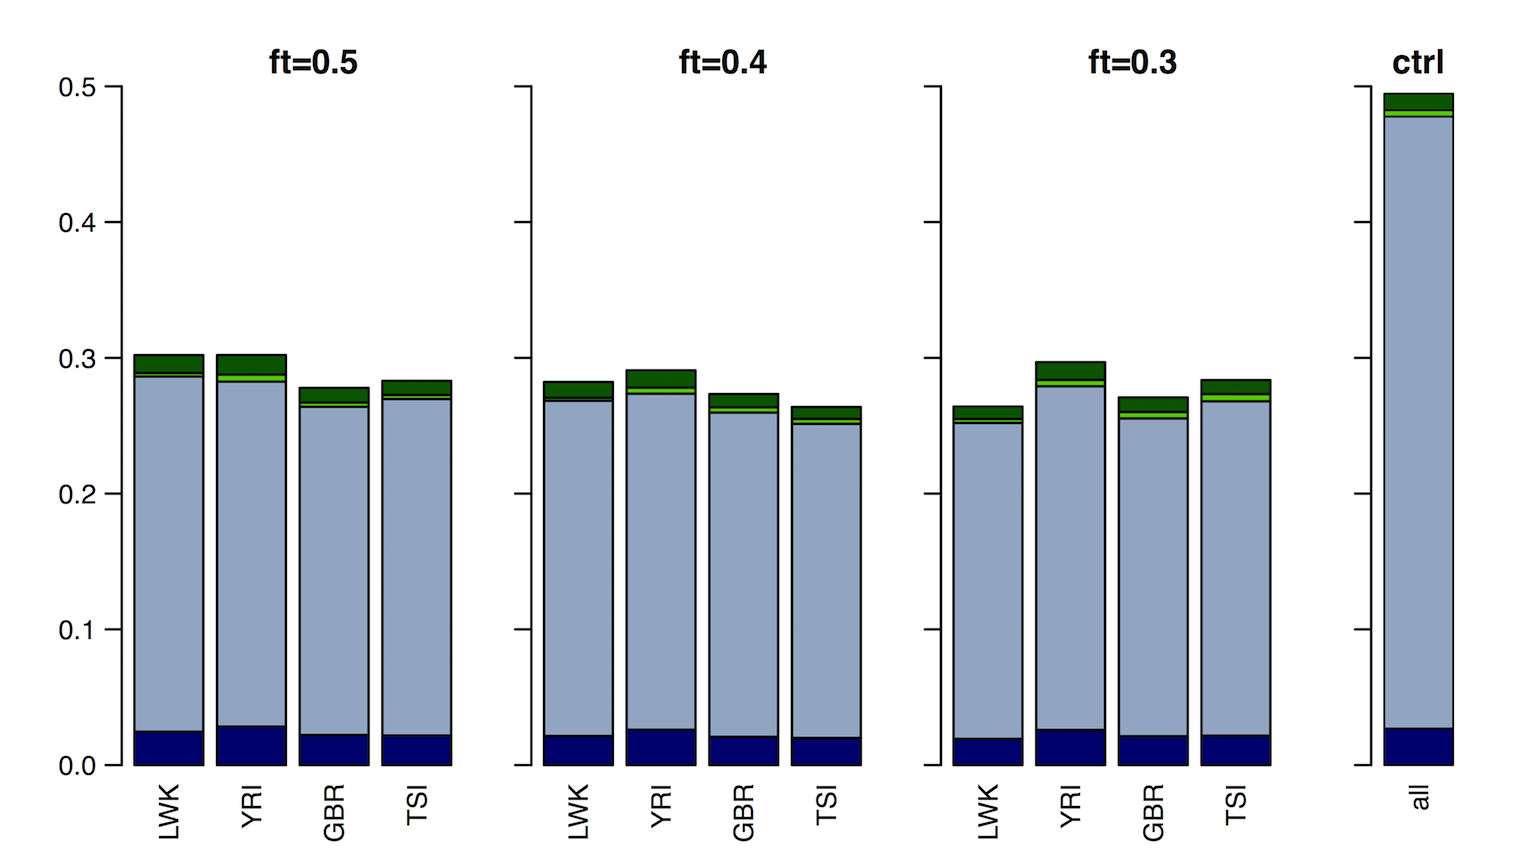
\includegraphics[]{chap2_folder/supp_figures/S15_Fig.png}
\caption*{\textbf{Fig S15. Proportion of sequences pertaining to each functional category.}
y-axis, the proportion of sequences over the total that belong to each category. x-axis, sets of significant windows for YRI, LWK, GBR and TSI (see Methods). all, all queried windows. darkblue=exon, lightblue=intron, lightgreen=3’UTR, darkgreen=5’UTR.
}
\end{figure}
%
\newpage
\begin{sidewaysfigure}[hp]
\centering
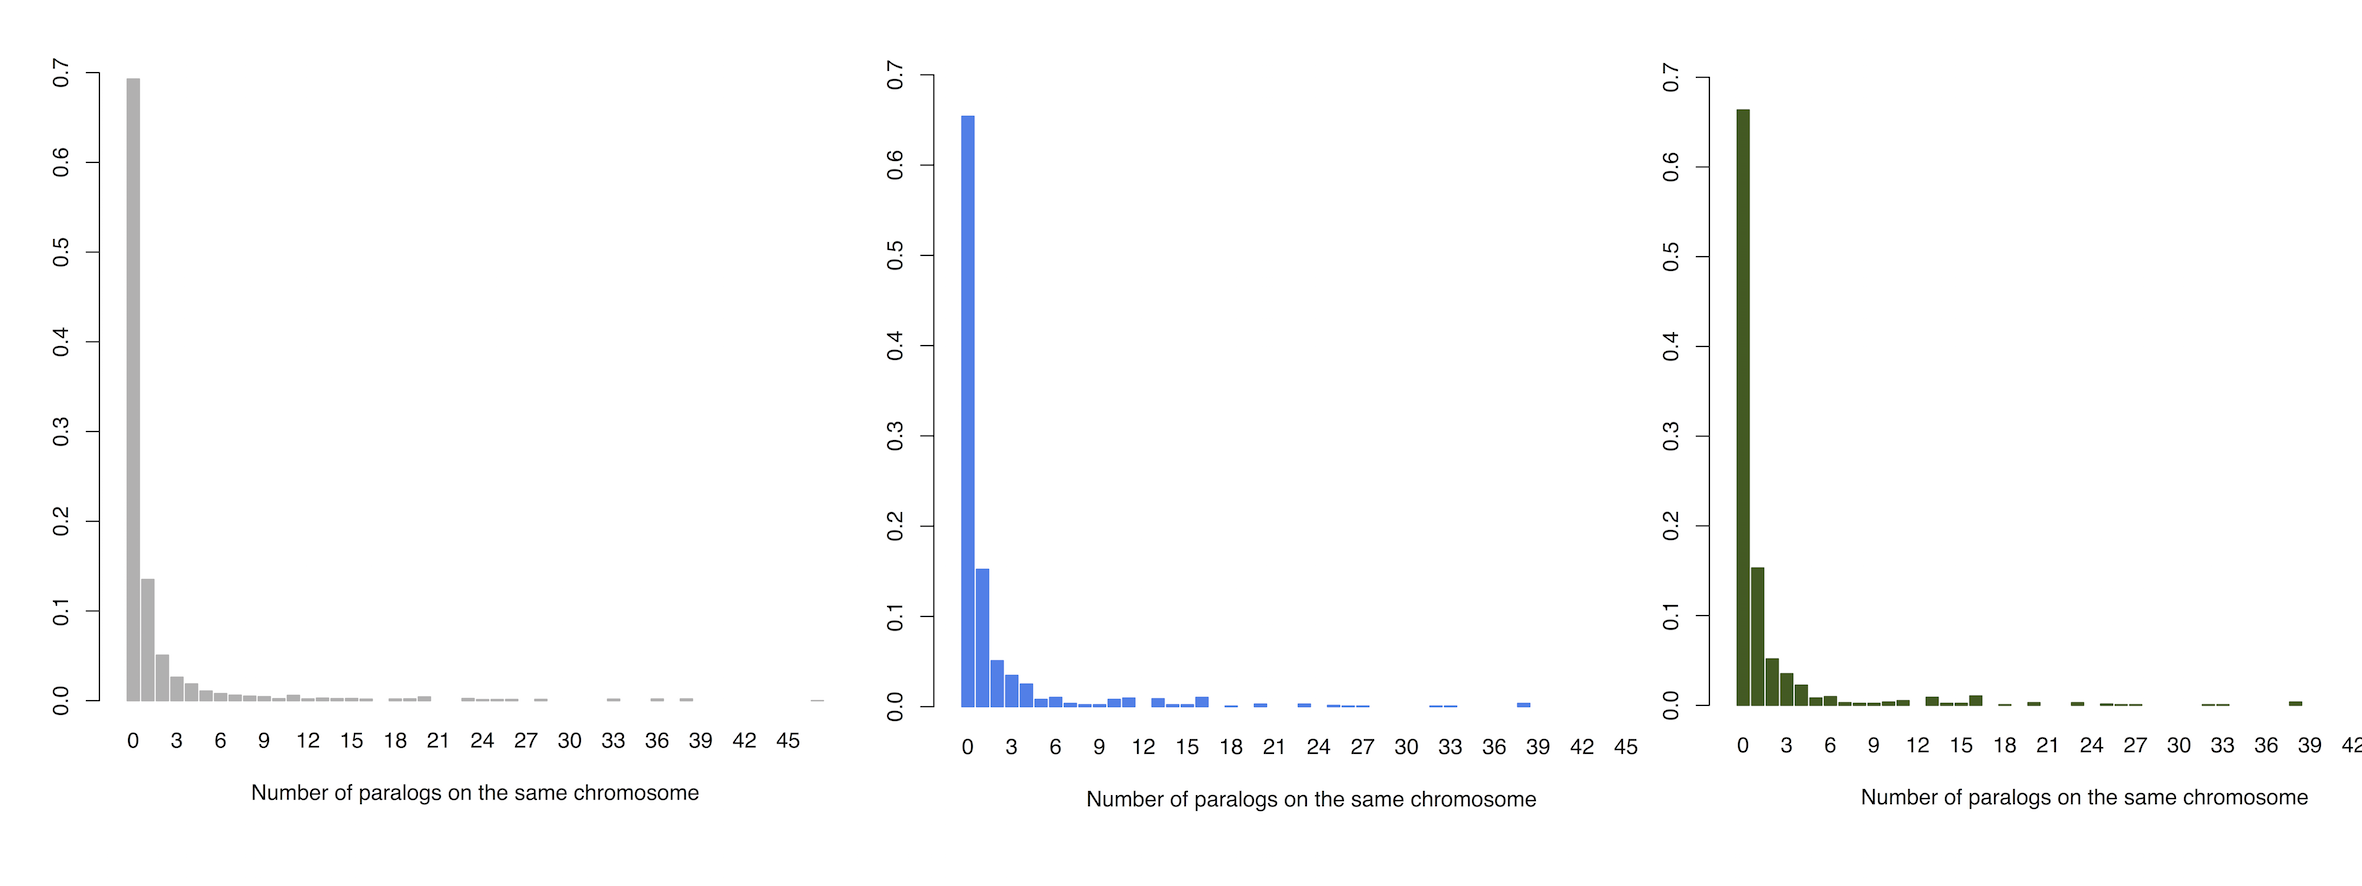
\includegraphics[]{chap2_folder/supp_figures/S16_Fig.png}
\caption*{\textbf{Fig S16. Number of paralog genes per gene on the same chromosome.}
For each protein-coding gene from human autosomes (19,349), the number of paralogs present in the same chromosome is plotted (left, gray). All autosomes come from Ensembl for hg19, regardless if they were queried or not for $NCD2$. Significant genes (middle, blue) come from the union of significant genes for YRI considering all $tf$ values (see Table 2 in main paper). Significant genes without olfactory receptor genes (21 ORs in total) are shown on the right (green). y-axis, relative frequency of the genes that contain a given number of paralogs on the same chromosome. Note that the distributions are very similar for the background and significant genes.
}
\end{sidewaysfigure}
%%%%%%%%%%%%%%%%%%%%%%%%
%%%%%%%%%%%%%%%%%%%%%%%%

\begin{figure}[!htb]
\centering
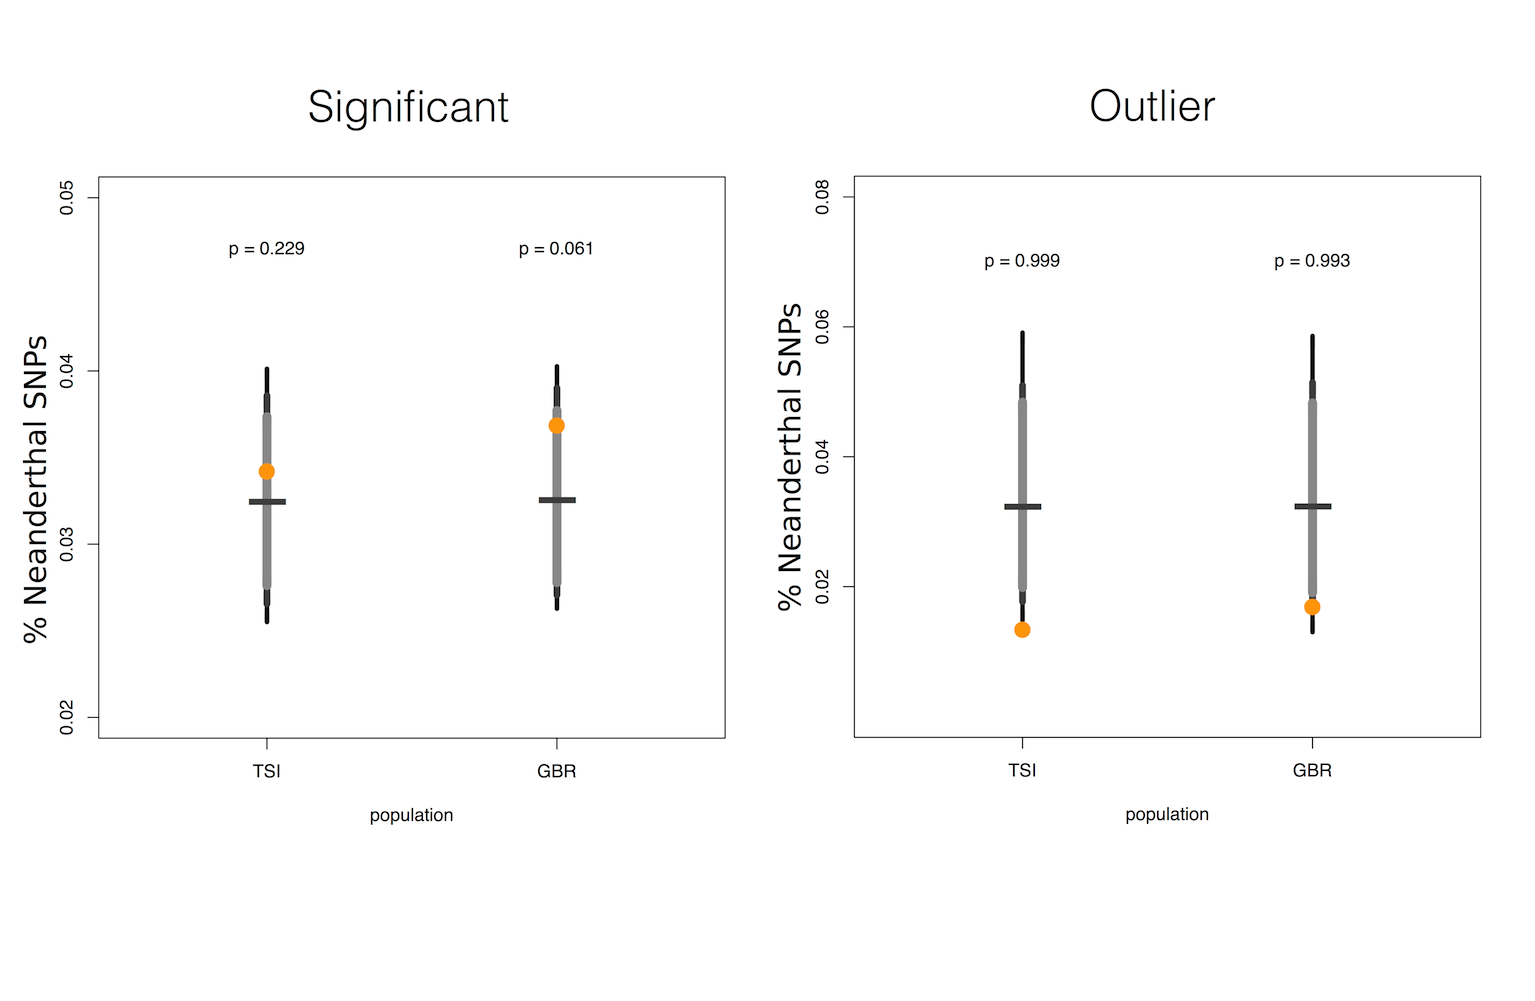
\includegraphics[]{chap2_folder/supp_figures/S17_Fig.png}
\caption*{\textbf{Fig S17. Proportion of Neanderthal SNPs in the candidate windows.}
Left, significant windows; right, outlier windows. In gray, distribution obtained from 1,000 samplings from the background. In orange, \% of Neanderthal SNPs within all significant (or outlier) windows. TSI, Toscani; GBR, Great Britain.
}
\end{figure}
%
%

\begin{sidewaysfigure}[!htb]
\centering
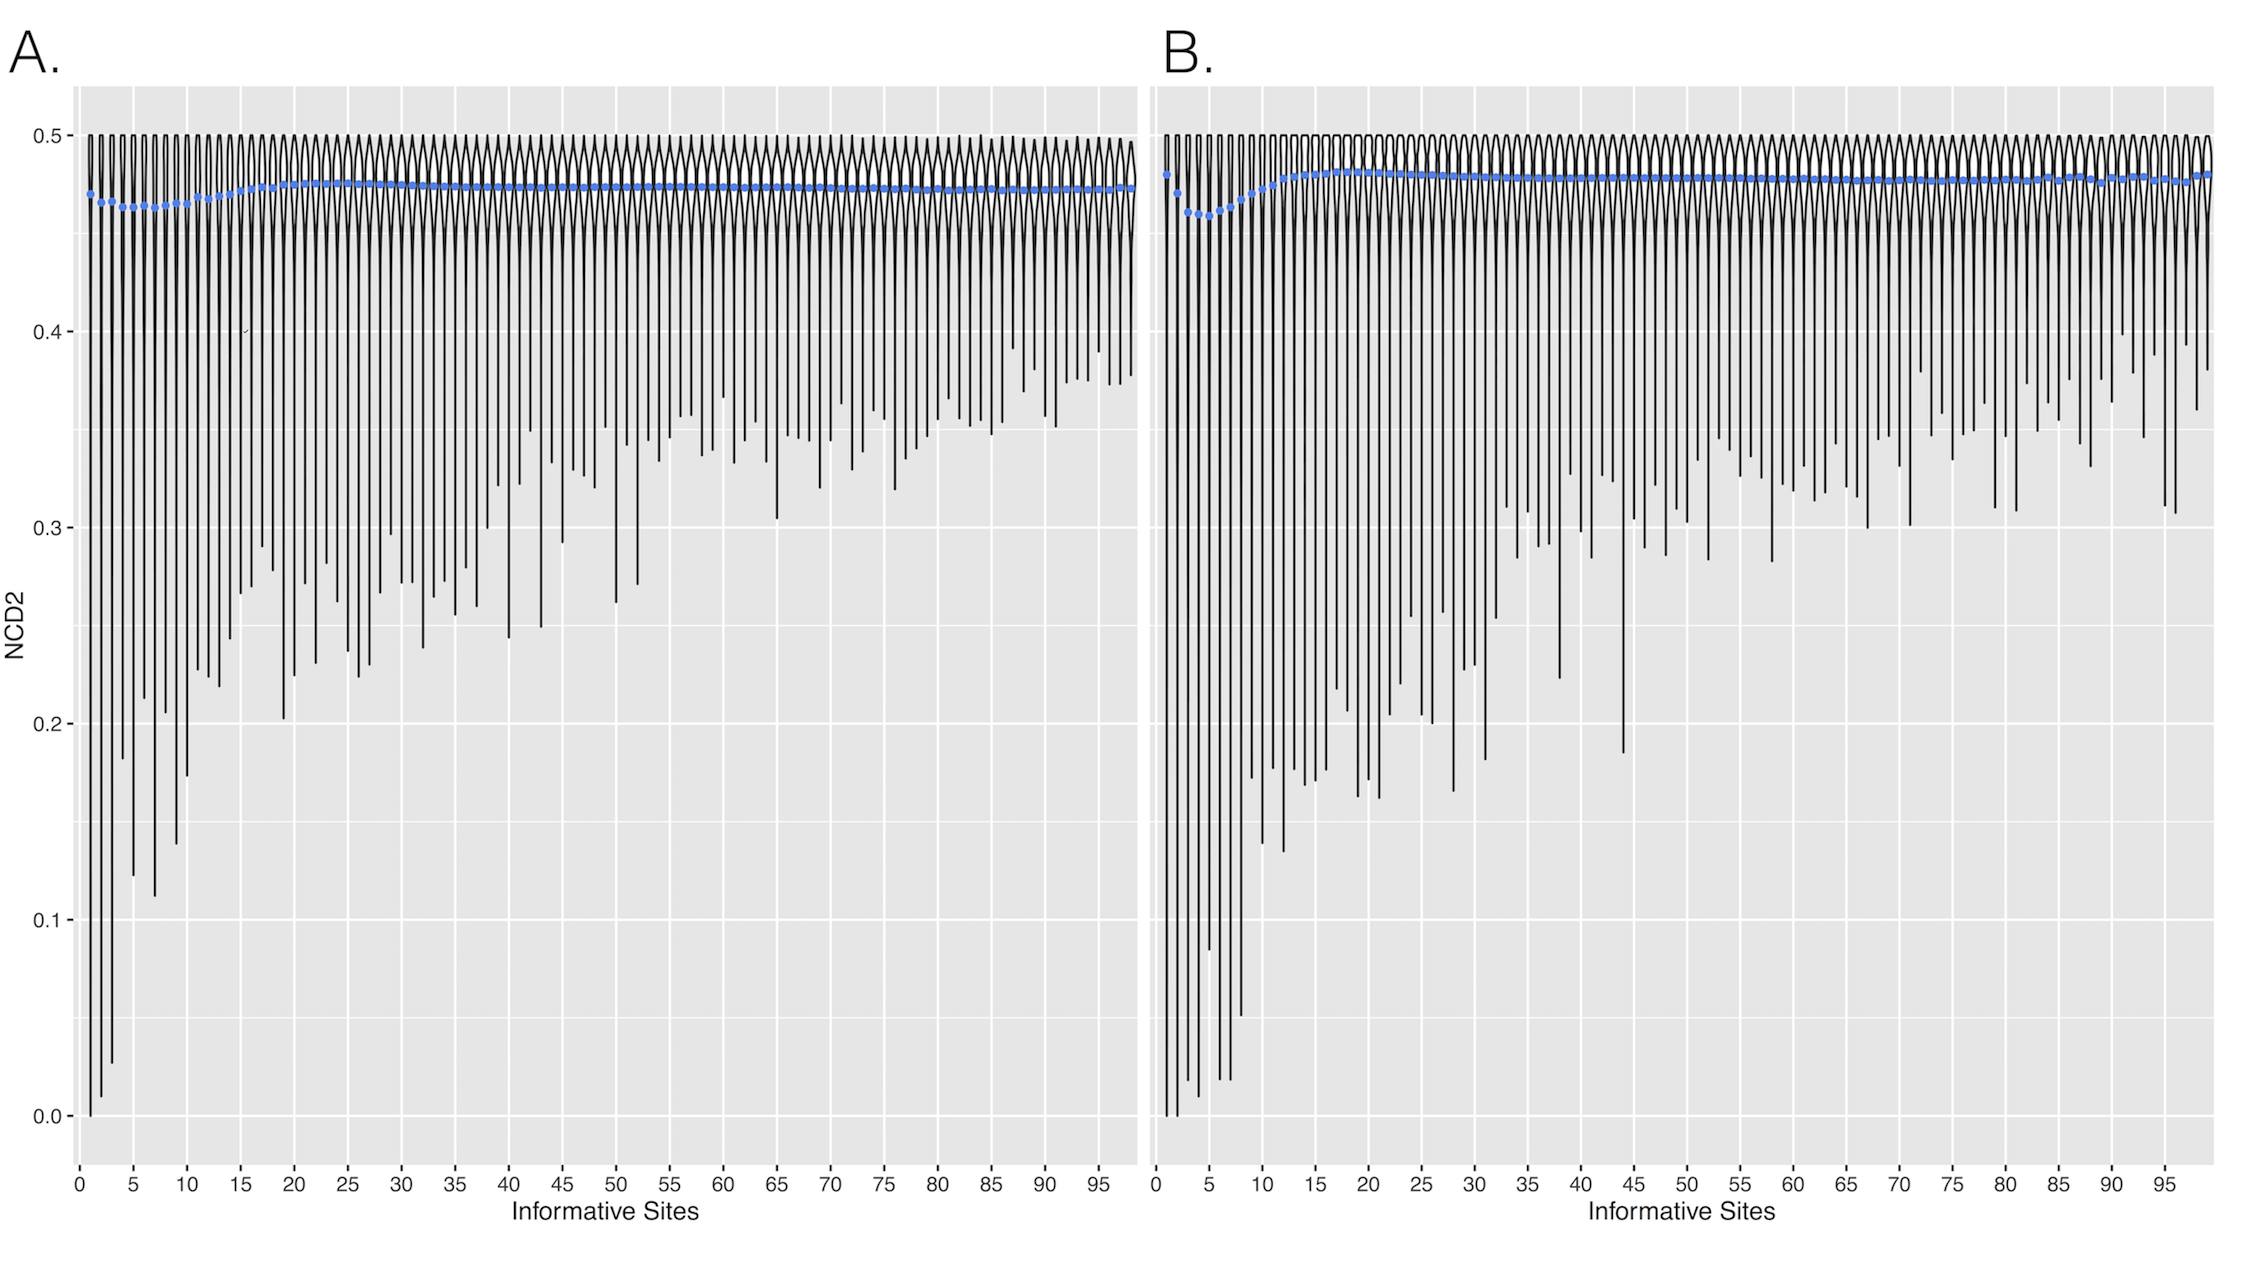
\includegraphics[]{chap2_folder/supp_figures/S18_Fig.png}
\caption*{\textbf{Fig S18. $NCD2_{0.5}$ empirical values for each bin of informative sites, IS.}
A) $NCD2_{0.5}$ for windows with IS between 1 and 100 for YRI (>99\% of all windows); B) $NCD2_{0.5}$ for all windows with IS between 1 and 100 for GBR (>99\% of all windows). In blue, median value for all the windows within a given bin. Note that the medians stabilize around 20 IS for YRI and around 15 IS for GBR.
}
\end{sidewaysfigure}
%
%
\begin{figure}[!htb]
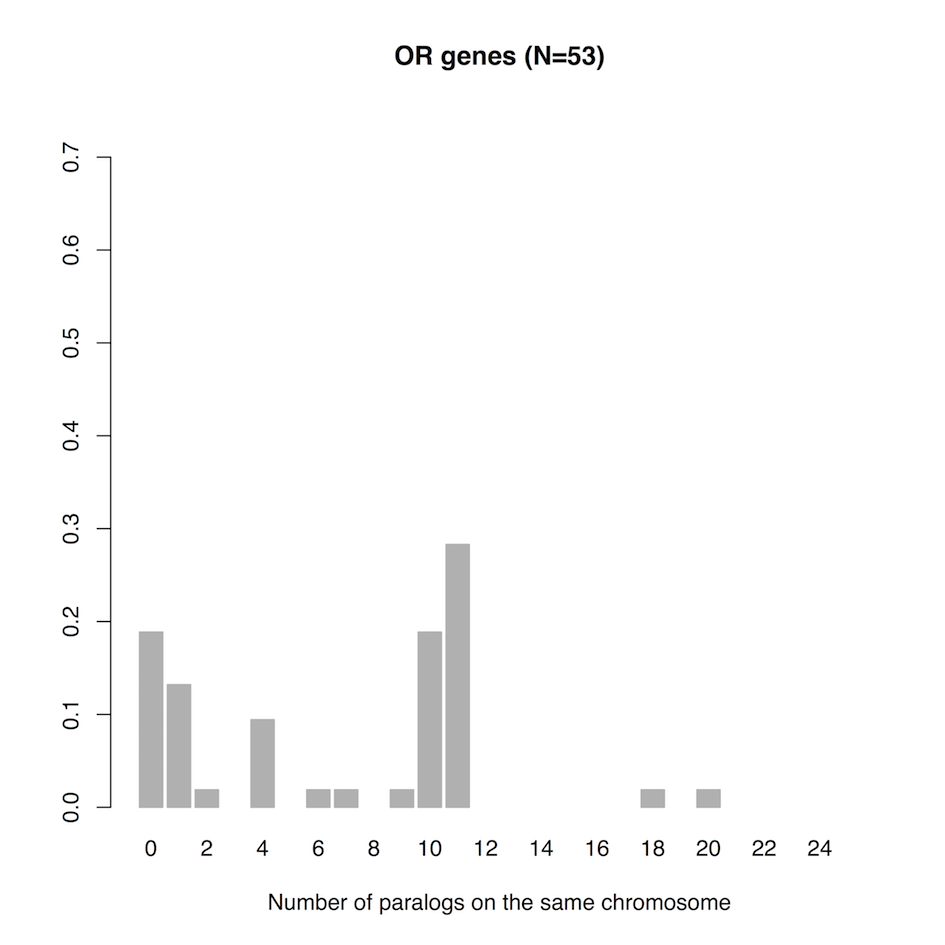
\includegraphics[]{chap2_folder/supp_figures/S19_fig.png}
\caption*{\textbf{Fig S19. Number of paralog genes per gene on the same chromosome.}
For each OR gene contained within any of the significant sets of windows (all populations and $tf$ values, 53 ORs in total), the number of paralogs present in the same chromosome is plotted. y-axis, relative frequency of the genes that contain a given number of paralogs on the same chromosome. Compare with distributions in S16 Fig.
}
\end{figure}
%
\begin{figure}[!htb]
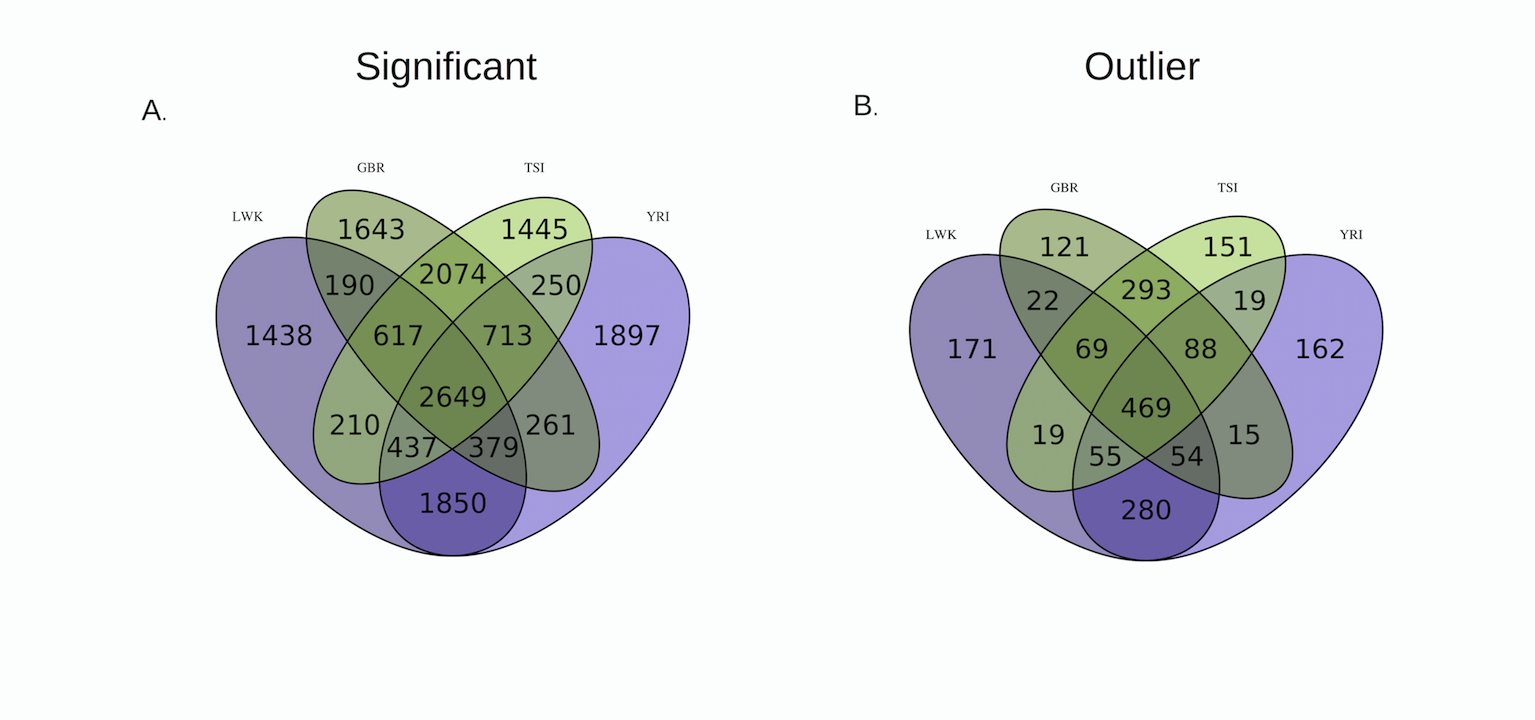
\includegraphics[]{chap2_folder/supp_figures/S20_Figure.png}
\caption*{\textbf{Fig S20. Venn diagrams of candidate windows for four populations.}
A, left, significant windows; B, right, outlier windows; YRI, Yoruba; LWK, Luhya; GBR, Great Britain; TSI, Toscani. The set of significant windows for each population comes from the union of significant and outlier windows for tf={0.3, 0.4, 0.5} (see Results and Methods). African populations are shown in tones of purple, and European in tones of green.}
\end{figure}
%should replace ft for td in this figure.
\begin{sidewaysfigure}[!htb]
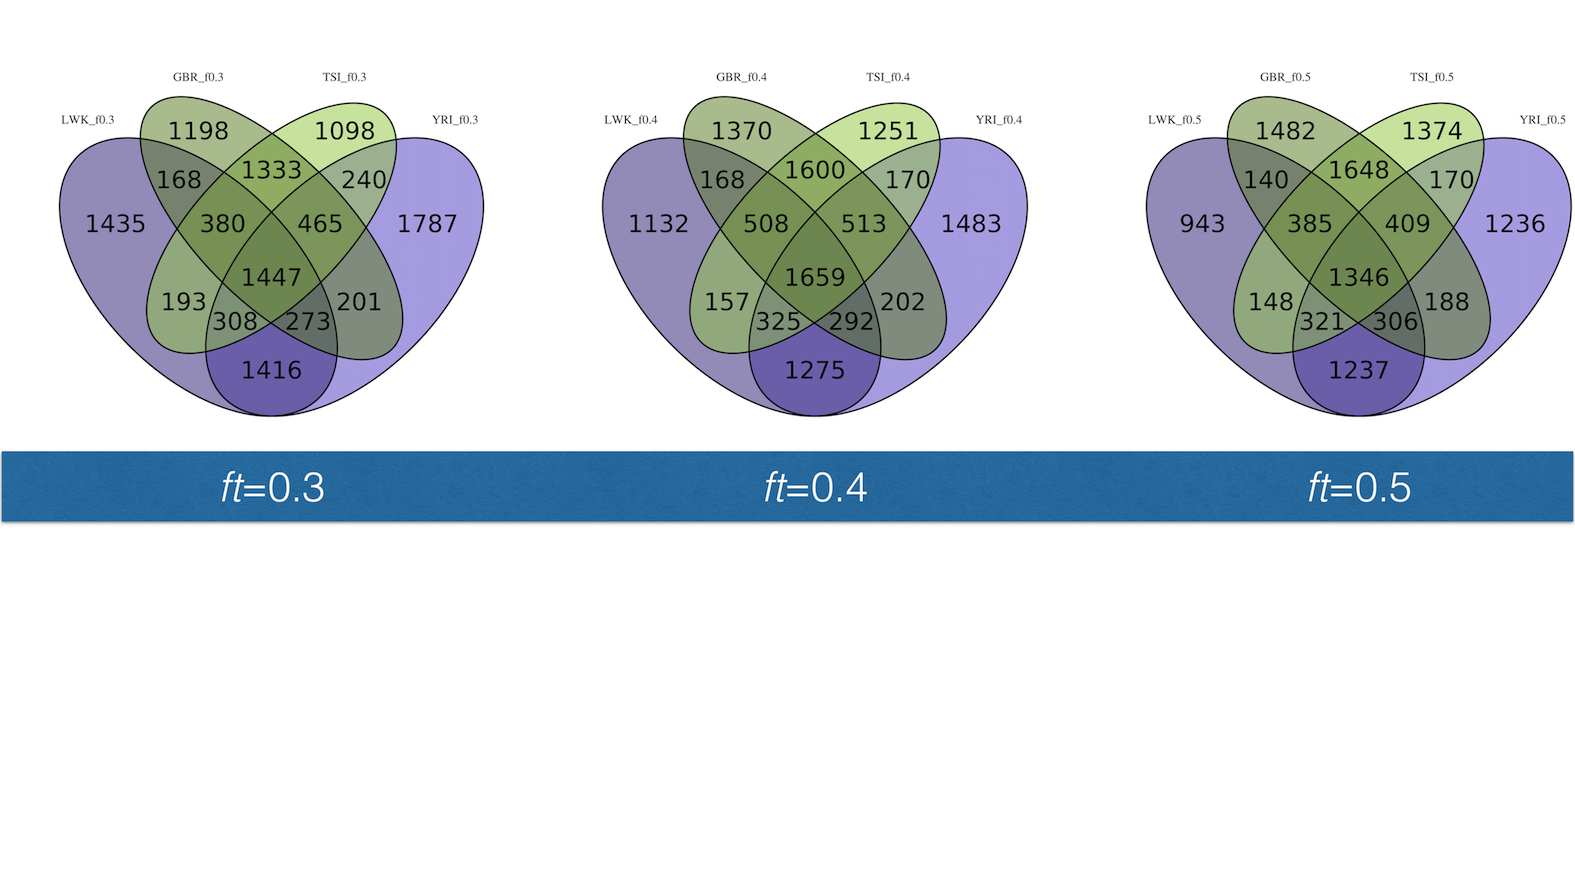
\includegraphics[]{chap2_folder/supp_figures/S21_Fig.png}
\caption*{\textbf{Fig S21. Venn diagrams of significant windows for four populations, for each $tf$ value. }
A, left, significant windows; B, right, outlier windows; YRI, Yoruba; LWK, Luhya; GBR, Great Britain; TSI, Toscani. The set of significant windows for each population comes from from those detected with each $tf$ value. African populations are shown in tones of purple, and European in tones of green.
}
\end{sidewaysfigure}
%Should replace ft for td in this figure
\begin{sidewaysfigure}[!htb]
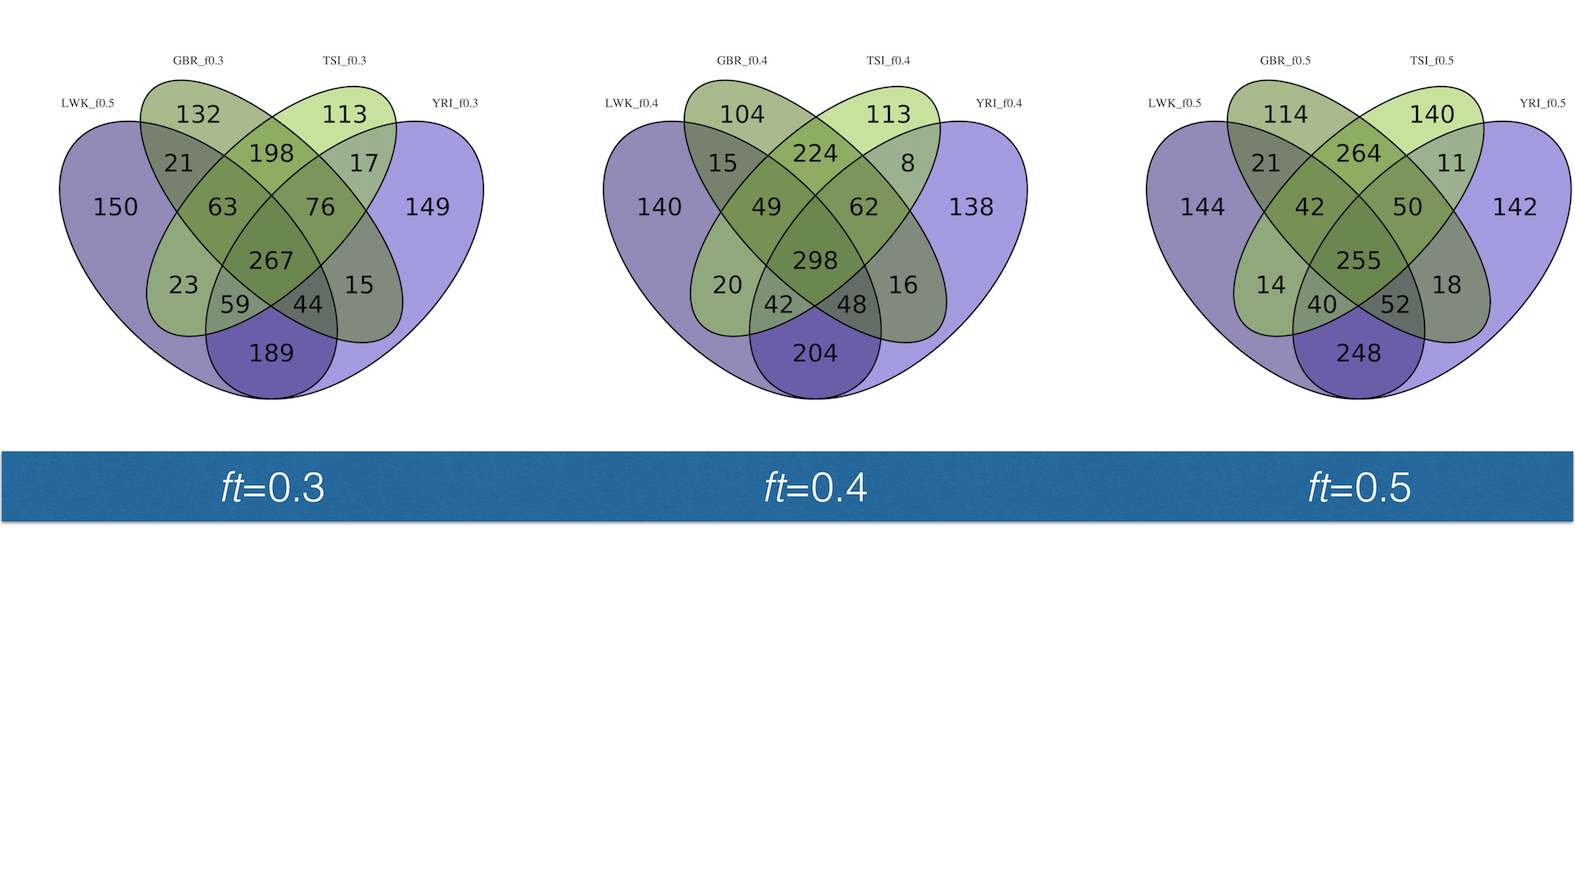
\includegraphics[]{chap2_folder/supp_figures/S22_Fig.png}
\caption*{\textbf{Fig S22. Venn diagrams of outlier windows for four populations, for each $tf$ value. }
A, left, significant windows; B, right, outlier windows; YRI, Yoruba; LWK, Luhya; GBR, Great Britain; TSI, Toscani. The set of significant windows for each population comes from from those detected with each ft value. African populations are shown in tones of purple, and European in tones of green.
}
\end{sidewaysfigure}
%

%\afterpage{\FloatBarrier}
%%%%%%%%%%%%%%%%%%%%%%%%%%%%%%%%%%%%%%%%%%%%%%%%%%%%%%%%%%%%%%%%%%%%%%%%%%%%%%%%%%%%%%%%%%%%%%%%%%%%%%%%%%%%%%%%%%%%%%%%%%%%%%%%%%%%%%%%%%%%%%%%%%%%%%%%%%%%%%%%%%%%%%%%%%%%%%%%%%%%%%%%%%%%%%%%%%%%%%%%%%%%%%%%%%%%%%%%%%%%%%%%%%%%%%%%%%%%%%%%%%%%%%%%%%%%%%%%%%%%%%%%%%%%%%%%%%%%%%%%%%%%%%%%

%%%%%%%%%%%%%%%%%%%%%%%%%%%%%%%%%%%
%%%%%%%%%%%%%%%%%%%%%%%%%%%%%%%%%%%
\end{otherlanguage}
\end{refsection}



\begin{refsection}
\chapter{Acúmulo de mutações deletérias em genes que foram alvos de seleção balanceadora de longo prazo em humanos}
%\addcontentsline{toc}{chapter}{Capítulo 2: Accumulation of deleterious mutations in regions under balancing selection}

\fancyfoot[C]{\thepage}
\rhead{Capítulo 2}
\counterwithout{equation}{chapter}
\setcounter{equation}{0}
\counterwithout{figure}{chapter}
\setcounter{figure}{0}
\counterwithout{table}{chapter}
\setcounter{table}{0}
%%%%%%%%%%%%%%%%%%%%%%%%%%%%%%%%%%%%%%%%%%%%%%%%%%%%%%%%%
\section{Considerações Iniciais}

Na última década -- e particularmente nos últimos 5 anos -- diversos trabalhos vêm documentando
a existência de uma parcela relativamente elevada de mutações deletérias em populações humanas. Alguns estudos encontraram 
uma diferença entre a carga genética de populações africanas e não-africanas (\cite{Hodgkinson2013,Lohmueller2008,Lohmueller2014,Henn2016}), ao passo que outros trabalhos vêm contestando tais achados (\cite{Do2015,Simons2014}). Paralelamente, uma série de estudos avaliaram a influência que as \enquote{varreduras seletivas} têm sobre variantes neutras próximas -- reduzindo a diversidade -- e, menos frequentemente, sobre variantes não-neutras -- limitando a eficácia da seleção nos sítios ligados (\cite{Betancourt2002,Chun2011}). Até o momento, nenhum estudo buscou avaliar o impacto que a seleção para a manutenção de um polimorfismo balanceado tem sobre variantes deletérias ligadas (exceto para HLA, \cite{Lenz2016}). Assim, buscamos testar a hipótese de que a seleção balanceadora sobre um sítios aumenta a abundância de alelos deletérios ligados que, na ausência de seleção balanceadora, poderiam ter sido eliminados por seleção purificadora. 

A fim de abordar essa questão, valemo-nos dos genes com assinaturas de seleção balanceadora identificados no Capítulo 1\footnote{Referimo-nos neste Capítulo ao manuscrito (não publicado) do Capítulo 1 como Bitarello et al. (n.d).}. Neste trabalho tive a colaboração de Débora Y.C. Brandt (doutoranda, Universidade da Califórnia, Berkeley) e Jônatas E. César (pós-doutorando, Universidade de São Paulo, IB), além de Diogo Meyer, que orientou o trabalho. D.Y.C.B. organizou os dados do Projeto 1000 Genomas para nossas análises, calculou as frequências alélicas por população e contribuiu com anotações funcionais para os SNPs. J.E.C. desenvolveu \emph{scripts} eficientes para as abordagens de re-amostragem descritas no manuscrito, além de ter feito o pré-processamento dos dados para nossas análises. Eu participei de todas as etapas descritas, fiz o planejamento das análises a serem feitas (juntamente com D.M. e J.E.C.) e redigi o manuscrito, juntamente com D.M., com colaboração e aprovação dos outros co-autores. Todos contribuíram para a discussão dos resultados. Pretendemos submetê-lo para o periódico \emph{Genetics}.

%%%%%%%%%%%%%%%%%%%%%%%%%%%%%%%%%%%%%%%%%%%%%%%%%%%%%%%%%%%%%%%%%%%%%%%%%%%%%%%%%%%%%%%%%%%%%%%%%%%%%%%%%%%%%%%%%%%%%%%%%%%%%%%%%%
\newpage
\begin{otherlanguage}{english}

\begin{center}

\LARGE{Balancing selection drives the accumulation of linked deleterious variation in humans}


\end{center}

\begin{center}
Bárbara Domingues Bitarello\textsuperscript{1}, Jônatas Eduardo César\textsuperscript{1}, Débora Yoshihara Caldeira Brandt\textsuperscript{2}, Diogo Meyer\textsuperscript{1}
\end{center}

\footnotesize{1, Departamento de Genética e Biologia Evolutiva, Universidade de São Paulo, São Paulo, Brazil}

\footnotesize{2, University of California, Berkeley, USA} 
%%%%%%%%%%%%%%%%%%%%%%%%%%%%%%%%%%%%%%%%%%%%%%%%%%%%%%%%%%%%%%%%%%%%%%%%%%%%%%%%%%%%%%%%%%%%%%%%%%%%%%%%%%%%%%%%%%%%%%%%%%%%%%%%%%
%%%%%%%%%%%%%%%%%%%%%%%%%%%%%%%%%%%%%%%%%%%%%%%%%%%%%%%%%%%%%%%%%%%%%%%%%%%%%%%%%%%%%%%%%%%%%%%%%%%%%%%%%%%%%%%%%%%%%%%%%%%%%%%%%%%%%%%%%%%%%%%%%%%%%%%%%%%%%%%%%%%%%%%%%%%%%%%%%%%%%%%%%%%%%%%%%%%%%%%%%%%%%%%%%%%%%%%%%%%%%%%%%%%%%%%%%
%%%%%%%%%%%%%%%%%%%%%%%%%%%%%%%%%%%%%%%%%%%%%%%%%%%%%%%%%%%%%%%%%%%%%%%%%%%%%%%%%%%%%%%%%%%%%%%%%%%%%%%%%%%%%%%%%%%%%%%%%%%%%%%%%%

%
\normalsize
\section{Introduction}
\lettrine[lines=3]{\color{airforceblue}U}{nderstanding} the dynamics and factors that interfere with the efficacy of natural selection is crucial to understanding phenotypes, complex diseases and genome structure in humans (\cite{Brandvain2016}). Mutations \emph{per se} can be neutral, advantageous, slightly deleterious or strongly deleterious and genomic studies have shown that human populations harbour a large number of deleterious mutations (e.g. \cite{Eyre-Walker1999,Kiezun2013}, among several others). 

Using comparative methods, \textcite{Eyre-Walker1999} estimated that about 1.6 new deleterious mutations arise per human individual per generation. %%this sentence came  from Lohmueller, I need to rephrase and add more references so it doesnt look identical. Perhaps it is unnecessary.
Estimates of load carried per individual vary between three to five (\cite{Morton1956}) and as much as 100 lethal equivalents (\cite{Kondrashov1995}) -- i.e, an allele or combination of alleles that if made homozygous would be lethal (\cite{Lohmueller2008}). More recent estimates vary from 300 to 1,200 deleterious mutations per diploid (human) genome (\cite{Fay2011,Lohmueller2008,Sunyaev2001}). %check these estimates. check if this is not too similar to lohmueller.
All of these estimates mostly reflect the assumed mutation rate, but also rely on effective population size, dominance, and the assumption that populations are in equilibrium (\cite{Brandvain2016}). Moreover, the methods used in the determination of what makes a mutation \enquote{deleterious} vary considerably (reviewed in \cite{Henn2015a}). Therefore, it is possible that many analyses on the load of deleterious mutations carry inaccuracies (reviewed in \cite{Brandvain2016}).

Three  processes have a central role in accounting for the abundance and distribution of deleterious mutations in the genome:  mutation, drift, and selection (\cite{Brandvain2016}). Firstly, the balance between influx via mutation and removal via purifying selection results in a dynamic process, where a large number of weakly selected variants can be maintained at low frequencies. Exome and genome-wide studies reporting an enrichment of recent deleterious mutations are strong evidence for this process (\cite{Casals2013,Fu2012,Tennessen2012,Kiezun2013}).

Secondly, features of a population's demographic history can influence the load of deleterious mutations that it carries. The last decade has seen an explosion of studies comparing the genetic load between human populations (\cite{Tishkoff2002,Lohmueller2008,Lohmueller2014,Simons2014,Henn2015a,Henn2016}). \textcite{Lohmueller2008} quantified the number of deleterious mutations per diploid genome in African American (AA) and European Americans (EA) individuals, finding that EA individuals have lower levels of nucleotide heterozygosity for all functional categories analysed, and a higher number of homozygous genotypes for derived alleles in synonymous and nonsynonymous sites and for "possibly damaging" (\cite{Adzhubei2010}) SNPs.

Although the former result is compatible with a rich body of literature documenting decreasing levels of heterozygosity with increasing distance from Africa (e.g.\cite{Tishkoff2002,Henn2015a}), the second observation is not, \emph{a priori}, expected. Moreover, among the SNPs segregating in only one of the two populations, the proportion of nonsynonymous SNPs was found to be significantly higher in EA (\cite{Lohmueller2008}).

This excess of deleterious mutations in European populations was interpreted as a consequence of a recent out-of-Africa bottleneck ($\sim 50,000$ years ago) followed by explosive population growth until the present (\cite{Lohmueller2008}). Although the African population also experienced  growth, it happened further in the past and thus this population would have had enough time to move closer to equilibrium conditions (\cite{Lohmueller2008}). Later findings supported this hypothesis (\cite{Alkan2009,Subramanian2012,Subramanian2016,Hodgkinson2013,Peischl2013,Peischl2015}), while others disputed it (\cite{Do2015,Simons2014}). 

A third factor that can account for the load in our genomes is pleiotropy, which is widespread in the human genome. For example, several studies show that disease alleles are often also positively selected, indicating that a deleterious variant has been pushed to a high frequency due to some other contribution to fitness it displays (e.g. \cite{Corona2010}). %perhaps mention autoimmune diseases associadtes to HLA?

Here, we explore an additional process that can play a role in shaping the load of mutations: the effect of selection on closely linked loci. It is plausible that at least part of the mutational load in humans is due not to demographic factors, but to indirect consequences of selection in adjacent loci (Figure ~\ref{fig:schema}).

%%%%%%%% Figure %%%%%%%%%%%
%%%%%%%% Figure %%%%%%%%%%%
\begin{figure}[ht]
\centering
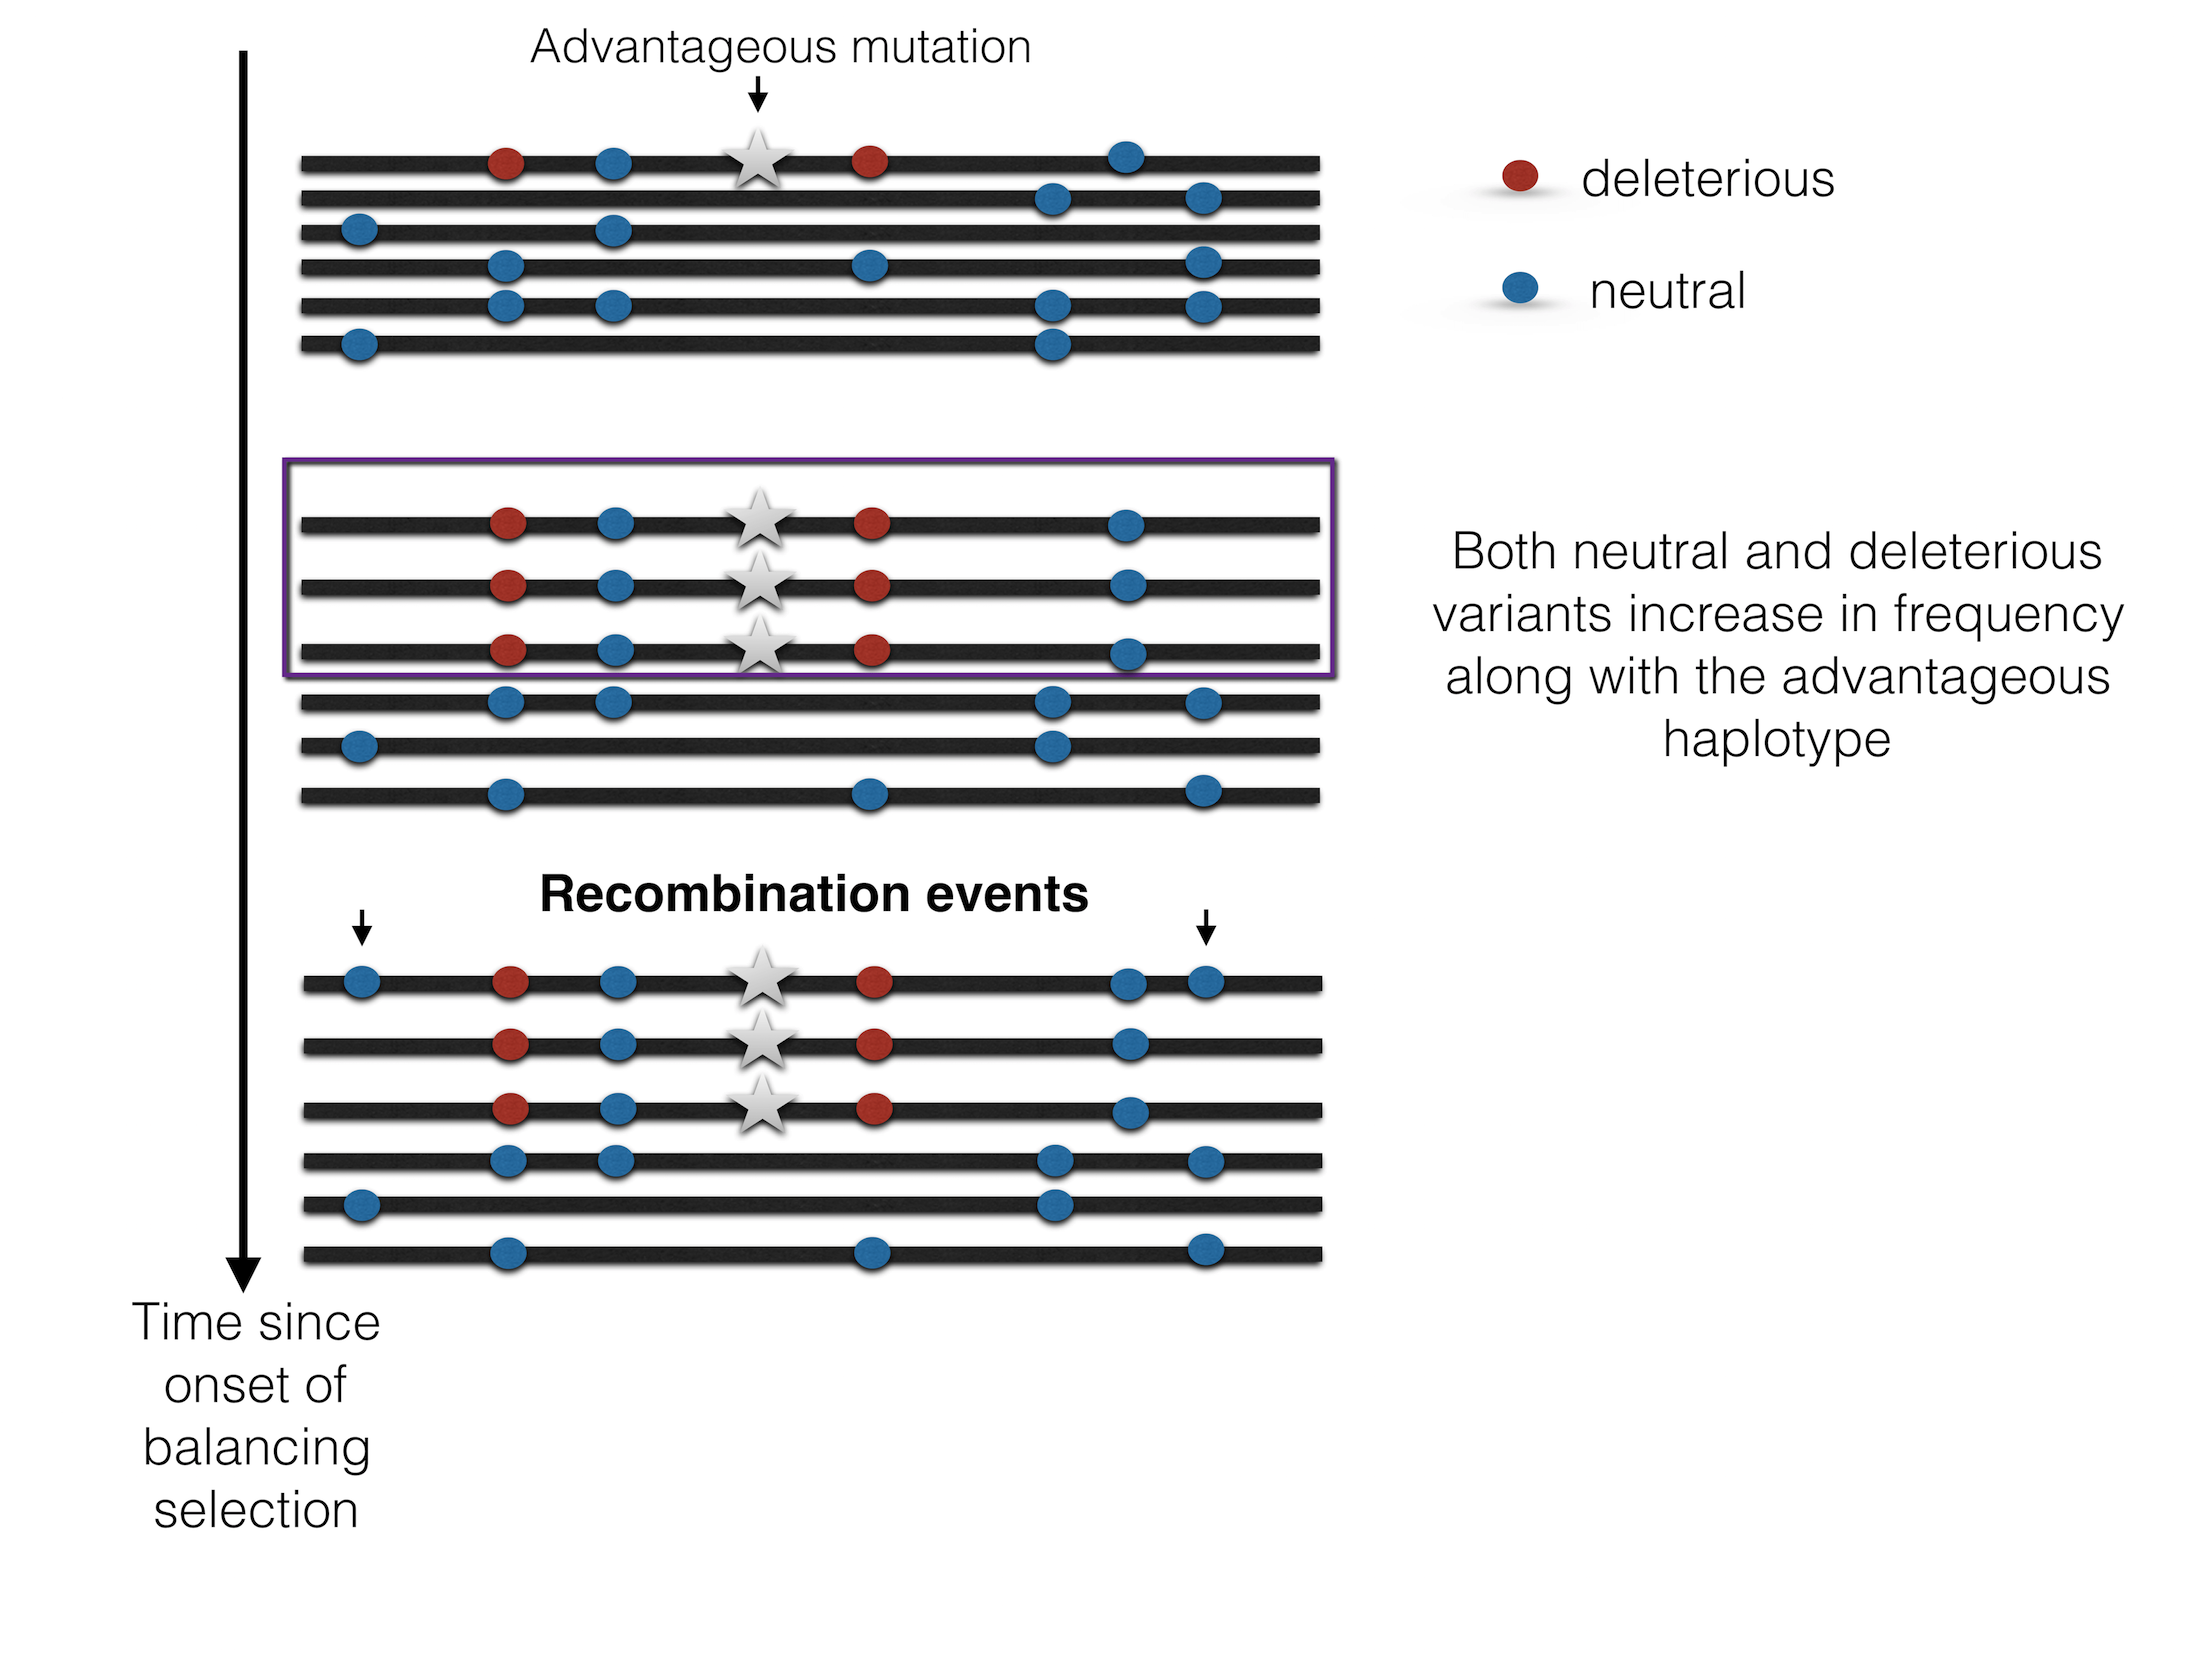
\includegraphics[width=13 cm, keepaspectratio]
{chap3_folder/figures/FIG_1_chap2_tiny.png}
\caption{\textbf{Effect of balanced polymorphism on neighboring sites.} When an advantageous variant appears in a given haplotype, but the site itself is under long-term balancing selection, the advantageous variant increases the frequency of neutral and deleterious variants in linkage. Because two or more haplotypes are maintained, the linked variants are also kept polymorphic. Adapted from \textcite{Charlesworth2006}.}
\label{fig:schema}
\end{figure}
%%%%%%%% Figure %%%%%%%%%%%
%%%%%%%% Figure %%%%%%%%%%%

In this study we take up the task of understanding how  balancing selection in humans has shaped the level of load in adjacent loci. It is well understood how selection -- directional and balancing -- has shaped neutral variation in regions that lie close to sites under either directional or balancing selection (e.g. \cite{Charlesworth2006,Charlesworth2012,Cutter2013,Nielsen2005}, to name a few). Recombination rates and neutral genetic diversity are correlated in several organisms (reviewed in \cite{Charlesworth2012,Cutter2013}) and, when selective sweeps occur, a depletion of neutral diversity is verified around the selected site (\cite{Charlesworth2012,Cutter2013,Nielsen2005}). The extent of this effect is a consequence of both recombination rates and the intensity of selection (\cite{Roux2013,schierup2000effect,Charlesworth1997}).

The effects of directional selection on the accumulation of deleterious mutations are less understood, but have also been addressed (e.g. \cite{Betancourt2002,Chun2011}). Interestingly, studies in \emph{Drosophila} have highlighted that strong purifying (background) selection  hampers the effectiveness of natural selection targeting neighboring sites: near strongly selected sites, there is increased accumulation of deleterious mutations and the effectiveness of selection targeting optimal codon usage is lower (\cite{Betancourt2002}). There is also evidence that directional selection limits the efficacy of purifying selection in neighboring sites in humans (\cite{Chun2011}).


All these findings suggest that there is a complex interaction of different selective forces targeting linked sites and possibly that linkage limits the efficiency of purifying selection in purging deleterious mutations from the genome. In this context, we propose to examine the following question: does balancing selection targeting certain sites in the human genome interfere with the effectiveness of natural selection in nearby sites, as has been observed for strong directional selection? 

From a theoretical point of view, a first expectation is that balancing selection would increase the rate at which deleterious mutations are purged from the genome. This expectation arises because balancing selection \textit{increases} the effective population size ($N_{e}$) of the genomic region under selection \parencite{Charlesworth1997,Roux2013,schierup2000effect}, and increased $N_{e}$ leads to an increase in the efficacy of natural selection. The key to understanding this apparent paradox is to consider that balancing selection often involves the occurrence of partial selective sweeps (i.e., there is an increase in frequency of the favored allele, but not to the point of fixation, followed by other such events, favoring other variants) \parencite{Connallon2013,Albrechtsen2010b}. Such a process enhances diversity, but variation is structured among haplotypes. This process is analogous to the increase in $N_{e}$
for a structured population, where each deme has a small $N_{e}$, but the overall meta-population has a large $N_{e}$ \parencite{Charlesworth1997,Roux2013,schierup2000effect}. Therefore, balancing selection should increase the genetic load in the vicinity of the balanced polymorphism.

To our knowledge, an increase in genetic load in the vicinity of targets of balancing selection has only  very recently been reported for HLA genes (\cite{Mendes2013,Lenz2016}) and has also been suggested for the \enquote{S} loci in \emph{Arabidopsis} and \emph{Solanum}. In \enquote{S} loci it was interpreted in the context of \enquote{sheltered load}, which relies on the assumption that deleterious variants are recessive and are less \enquote{seen} by purifying selection in regions of high heterozygosity (\cite{Stone2004,Roux2013}). 

Therefore, investigating whether an increased proportion of deleterious variants occurs for targets of balancing selection throughout the entire genome has not yet been examined except in the context of HLA genes. We address this question by investigating the levels of accumulation of deleterious mutations in regions surrounding sites previously detected as targets of balancing selection in a powerful genome-wide approach (\cite{Bitarello2016}). Given the broad range of methods that can be used to identify deleterious variants, and the fact that they are frequently not in agreement (reviewed in \cite{Henn2015a}), we opt to use three complementary approaches. Moreover, most deleteriousness measures are negatively correlated with allele frequencies, thus we explicitly consider the effects of allele frequencies in our analyses.

Our expectation, given the theoretical background outlined above, was that regions with evidence for balancing selection would show an enrichment of deleterious variants. In accord with this expectation we found  strong evidence for an increased proportion of nonsynonymous variants within genes with signatures of long-term balancing selection (LTBS), as well as evidence for an increased proportion of deleterious variants.  

%%%%%%%%%%%%%%%%%%%%%%%%%%%%%%%%%%%%%%%%%%%%%%%%%%%%%%%%%%%%%%%%%%%%%%%%%%%%%%%%%%%%%%%%%%%%%%%%%%%%%%%%%%%%%%%%%%%%%%%%%%%%%%%%%%
\section{Methods}

%%%%%%%%%%%%%%%%%%%%%%%%%%%%%%%%%%%%%%
%%%%%%%%%%%%%%%%%%%%%%%%%%%%%%%%%%%%%%
\subsection{Population datasets}
%%%%%%%%%%%%%%%%%%%%%%%%%%%%%%%%%%%%%%
%%%%%%%%%%%%%%%%%%%%%%%%%%%%%%%%%%%%%%

In order to test the hypothesis that sites within genes with evidence for long-term balancing selection (LTBS) show an excess of deleterious variants, we considered all protein-coding SNP positions (nonsynonymous, \emph{N}, and synonymous, \emph{S}) from the 1000 Genomes Phase 3 data (\cite{Auton2015}). We selected SNPs that fall within the  coordinates of genes with signatures of LTBS (\enquote{balanced genes}, see below) or  within the target windows \emph{per se} (\enquote{balanced windows}) (Tables ~\ref{tab:balancedSNPs} and ~\ref{tab:outlierSNPs}).

We used the integrated call sets in VCF format for each chromosome, and calculated reference and alternative allele frequencies per population using VCFtools (\cite{Danecek2011}). We only considered populations from Africa and Europe, and excluded the admixed ones, thus resulting in 10 populations: [Africa: Yoruba in Ibadan, Nigeria (YRI), Luhya in Webuye, Kenya (LWK), Mende in Sierra Leone (MSL), Gambian in Western Division, The Gambia (GWD), Esan in Nigeria (ESN)]; [Europe: Toscani in Italy (TSI), British in England and Scotland (GBR), Iberian populations in Spain (IBS), Finnish in Finland (FIN), Utah residents with Northern and Western European ancestry (CEU)]. We did not include Asian populations because the targets of balancing selection defined by \textcite{Bitarello2016} were only documented for African and European populations. 


%%%%%%%%%%%%%%%%%%%%%%%%%%%%%%%%%%%%%%%%%%%%%%%
%%% Table %%% Table %%% Table %%% Table %%% Table %%% Table 
%%% Table %%% Table %%% Table %%% Table %%% Table %%% Table 
%%% Table %%% Table %%% Table %%% Table %%% Table %%% Table

\begin{sidewaystable}[h]
\centering
\small
\begin{tabular}{@{}cccccccc@{}}
\toprule
 & \multicolumn{7}{c}{Balanced genes} \\ \midrule
\rowcolor[HTML]{9B9B9B} 
{\color[HTML]{000000} POP} & {\color[HTML]{000000} \# sites} & {\color[HTML]{000000} \emph{N}} & {\color[HTML]{000000} \emph{S}} & {\color[HTML]{000000} $P_{del1}$} & {\color[HTML]{000000} $P_{del2}$} & {\color[HTML]{000000} Benign} & {\color[HTML]{000000} Cscore} \\ \cmidrule(r){1-8}
YRI & 3,423(2,961) & \multicolumn{1}{l}{1,871(1,564)} & \multicolumn{1}{l}{1,552(1,397)} & \multicolumn{1}{l}{197(182)} & \multicolumn{1}{l}{262(238)} & \multicolumn{1}{l}{1,300(1,034)} & \multicolumn{1}{l}{10.72(11.36)} \\
LWK & 3,587(3,126) & 1,959(1,654) & 1,628(1,472) & 213(194) & 281(260) & 1,357(1,093) & 10.85(11.52)  \\
MSL & 3,387(2,937) & 1,837(1,543) & 1,550(1,394) & 198(184) & 241(222) & 1,273(1,013) & 10.63(11.26)  \\
GWD & 3,550(3,098) & 1,967(1,668) & 1,583(1,430) & 198(181) & 292(272) & 1,353(1,091) & 10.75(11.35)  \\
ESN & 3,261(2,821) & 1,804(1,517) & 1,457(1,304) & 202(187) & 265(248) & 1,238(984) & 10.91(11.63) \\
TSI & 2,596(2,146) & 1,479(1,181) & 1,117(965) & 175(161) & 230(211) & 997(733) & 10.88(11.82)  \\
GBR & 2,299(1,866) & 1,328(1,043) & 971(823) & 155(140) & 188(173) & 919(664) & 10.69(11.70) \\
FIN & 2,149(1,715) & 1,230(948) & 910(767) & 138(124) & 173(159) & 864(610) & 10.33(11.36) \\
CEU & 2,353(1,925) & 1,334(1,054) & 1,019(871) & 145(132) & 198(183) & 924(672) & 10.66(11.66)  \\
IBS & 2,612(2,153) & 1,507(1,200) & 1,105(953) & 171(155) & 237(216) & 1,034(764) & 10.82(11.71)  \\ \bottomrule
\end{tabular}
\caption{\textbf{Statistics for protein-coding SNPs  within the balanced genes}. Genes under balancing selection were defined by \textcite{Bitarello2016}. Numbers in parentheses refer to the datasets after removal of HLA genes (see Methods). Cscore, average scaled C score for all SNPs in the set (see Methods). $P_{N}$ and $P_{S}$, numbers of nonsynonymous and synonymous sites, respectively. $P_{del1}$, $P_{del2}$, and Benign, numbers of possibly damaging, probably damaging and benign variants (\cite{Adzhubei2010}), respectively.
}
\label{tab:balancedSNPs}
\end{sidewaystable}
%%%%%%%%%%%%%%%%%%%%%%%%%%%%%%%%%%%%%%%%%%%%%%%%%%%%%%%%%%%%%%%%%%%%%%%%%%%%%%%%%%%%%%%%%%%%%%%%%%%%%%%%%%%%%%%%%%%%%%%%%%%%%%%%%%%%%%%%%%%%%%%%%%%%%%%%%%%%%%%%%%

%%%%%%%%%%%%%%%%%%%%%%%%%%%%%%%%%%%%%%%%%%%%%%%%%%%%%%%%%
%%%%%%%%%%%%%%%%%%%%%%%%%%%%%%%%%%%%%%%%%%%%%%%%%%%%%%%%%

\subsection{Targets of balancing selection} 
%%%%%%%%%%%%%%%%%%%%%%%%%%%%%%%%%%%%%%%%%%%%%%%%%%%%%%%%%
%%%%%%%%%%%%%%%%%%%%%%%%%%%%%%%%%%%%%%%%%%%%%%%%%%%%%%%%%
%%%%%%%%%%%%%%%%%%%%%%%%%%%%%%%%%%%%%%%%%%%%%%%%%%%%%%%%%


	The "balanced genes" are those reported by \textcite{Bitarello2016} (see their Table 3) as having the strongest statistically significant signatures of LTBS in humans (213 genes in total). The list of balanced genes was generated by intersecting 3 Kb windows with strong signatures of LTBS with the protein-coding gene annotation from Encode/Ensembl (\cite{Bitarello2016}). Here we test the hypothesis of an enrichment in the proportion of deleterious variants in the balanced genes \emph{per se} (Table ~\ref{tab:balancedSNPs}). 

A more specific definition of the regions under balancing selection would involve the analysis of "balanced windows" (i.e., the queried sub-region of a gene with evidence for balancing selection, according to the method of \textcite{Bitarello2016}. However, this approach generates a dataset which is too restrictive (Table ~\ref{tab:outlierSNPs}), with a number of SNPs that is too small to provide reliable contrasts among regions under balancing selection with respect to the rest of the genome  (with on average 209 protein-coding SNPs per population, after the HLA genes are removed). We therefore chose to restrict our analyses to the balanced genes, for which we have a larger number of SNPs documenting the influence of selection on nearby sites.
% Seu ponto ficaria ainda mais forte se vocÊ reportasse o número de average number of "coding SNPs" per population, e não o total, pois aí daria para ver que para a análise de pn/ps e pdel/pneu o número realmente despenca.
%BDB;esse núemro é N+S, que eu acho que é o que você sugere, exatamente.


%In principle, testing for an enrichment of deleterious variants within the balanced windows would be restricting analyses to relatively narrow regions of the genome, for which there is strong evidence of balancing selection. This is consistent not only with what is expected for long-term balancing selection (\cite{Hudson1988,Charlesworth2006}), but also with human-specific demography, mutation and recombination rates  (\cite{Andres2009,Bitarello2016,Gravel2011,Roux2013}). 
% Eu acho que agora dá para tirar esse parágrafo e ir direto par ao próximo.

%When testing for an enrichment of deleterious variants within the whole gene for which we have evidence for balancing selection, our inquiry extends to a larger region than when focusing on the portion of the gene with evidence for being directly under balancing selection. There is a trade-off involved with these two approaches: window-based analyses contain few SNPs but correspond to regions with extreme deviations from neutrality; gene-based analyses are performed on a greater number of SNPs, but these are on average more distant from the site(s) of selection, and thus may include cases in which the effect of linked selection is weaker. Nevertheless, given that the windows used to detect targets of long-term balancing selection in \cite{Bitarello2016} are narrow (length of 3kb), the  gene-based approach (see below) has the advantage of directly measuring the effect of the  balanced polymorphisms within a gene over its nearby sites -- i.e, the remaining positions of the gene. 

% Eu acho que com a frase que eu propus esse trecho se torna desnecessário, pois já apresntei de cara a ideia de que o número de SNPs restrito sugere a remoção. Essa sugestão elimina um parágrafo inteiro (dois, na vereade), mas acho que ganhamos em clareza. E eu irei acrescentar material em outros lugares, de modo que o texto não corre risco de "encolher demais".
%BDB: ok...vou remover, mas acho que isso talvez não fique claro pra banca.

Our approach consists in a comparison of the number of deleterious SNPs within the genes under balancing selection and the remainder of the genome (which we refer to as providing a set of "control SNPs"). We define control SNPs as those protein-coding SNPs outside all balanced genes. We did not consider the SNPs contained in the sex chromosomes nor in the mitochondrial DNA since there is no information regarding balancing selection signatures for those genes (\cite{Bitarello2016}). More details about the controls are provided below in the "Re-sampling control SNPs" section. %check the name of this section at the end.

%%%%%%%%%%%%%%%%%%%%%%%%%%%%%%%%%%%%%%%%%%%%%%%%%%%%%%%%%%%%%%%%%%%%%%%%%%%%%%%%%

\begin{table}[h]
\centering
\small
\begin{tabular}{@{}cccccccc@{}}
\toprule
 & \multicolumn{7}{c}{Balanced windows} \\ \midrule
\rowcolor[HTML]{9B9B9B} 
{\color[HTML]{000000} POP} & {\color[HTML]{000000} \# sites} & {\color[HTML]{000000} \emph{N}} & {\color[HTML]{000000} \emph{S}} & {\color[HTML]{000000} $P_{del1}$} & {\color[HTML]{000000} $P_{del2}$} & {\color[HTML]{000000} Benign} & {\color[HTML]{000000} Cscore} \\ \cmidrule(r){1-8}
YRI & 635(225) & 401(124) & 234(102) & 23(9) & 30(9) & 333(93) & 7.50(9.26) \\
LWK & 651(236) & 400(122) & 251(114) & 29(12) & 28(8) & 332(9) & 7.34(9.07) \\
MSL & 636(234) & 391(124) & 245(110) & 20(7) & 29(10) & 327(93) & 7.52(9.29) \\
GWD & 652(248) & 406(136) & 246(112) & 29(13) & 35(16) & 328(93) & 7.88(9.91) \\
ESN & 630(235) & 387(125) & 243(110) & 28(13) & 24(8) & 321(91) & 7.46(9.43) \\
TSI & 612(205) & 388(113) & 224(92) & 27(13) & 33(15) & 317(75) & 7.62(9.93) \\
GBR & 561(171) & 361(100) & 200(71) & 24(9) & 28(14) & 302(70) & 7.25(9.31) \\
FIN & 553(166) & 351(91) & 202(75) & 22(8) & 24(10) & 297(65) & 7.02(8.80) \\
CEU & 559(172) & 353(96) & 206(76) & 19(6) & 28(14) & 297(67) & 7.17(9.29) \\
IBS & 607(196) & 384(107) & 223(89) & 26(11) & 33(15) & 314(70) & 7.46(9.58) \\ \bottomrule
\end{tabular}
\caption{\textbf{Statistics for protein-coding SNPs within balanced windows}. Windows are defined in \textcite{Bitarello2016}. Cscore, average scaled C score for all SNPs in the set (see Methods). $P_{N}$ and $P_{S}$, numbers of nonsynonymous and synonymous sites, respectively. $P_{del1}$, $P_{del2}$, and Benign, numbers of possibly damaging, propably damaging and benign variants, respectively (\cite{Adzhubei2010}).
}
\label{tab:outlierSNPs}
\end{table}
%%%%%%%%%%%%%%%%%%%%%%%%%%%%%%%%%%%%%%%%%%%%%%%%%%%%%%%%%
%%%%%%%%%%%%%%%%%%%%%%%%%%%%%%%%%%%%%%%%%%%%%%%%%%%%%%%%%
%%%%%%%%%%%%%%%%%%%%%%%%%%%%%%%%%%%%%%%%%%%%%%%%%%%%%%%%%%%%%%%%%%%%%%%%%%%%%%%%%%%%%%%%%%%%%%%%%%%%%%%%%%%%%%%%%%%%%%%%%%%%%%%%%%%%%%%%%%%%%%%%

%%%%%%%%%%%%%%%%%%%%%%%%%
\subsection{Annotation} 
%%%%%%%%%%%%%%%%%%%%%%%%%

One of the summary statistics used to quantify the genetic load was the CADD (Combined Annotation Dependent Depletion, or simply \enquote{C Score}) described in \textcite{Kircher2014}. Thus, we used the annotation provided in the study of \textcite{Kircher2014}  (available at: \url{http://cadd.gs.washington.edu/download}, accessed in March 2016).

From this annotation file we retrieved the following information: "CHR" (chromosome where the SNP is situated), "POS" (position of SNP in chromosome),  "Consequence" (nonsynonymous, synonymous, 3-prime-UTR, 5-prime-UTR, intronic, non-coding change, canonical splice,stop-gained, stop-lost),  "GeneName" (associated gene name to the SNP position), "AnnoType" (NonCodingTranscript, Transcript, CodingTranscript), "PolyPhenCat" (benign, possibly damaging, probably damaging), and the scaled and raw C scores (\cite{Kircher2014}). 

Because two of our measurements of genetic load (see below) are only applicable to protein-coding sites, we restricted our analyses to these categories. Thus, all quantification of deleterious load was restricted to sites which are protein-coding (i.e., \emph{N} or \emph{S}) (Tables ~\ref{tab:balancedSNPs} and ~\ref{tab:outlierSNPs}). For the step where we identified the specific SNPs with highest heterozygosity for each gene (and which is/are the putative target(s) of balancing selection, see below) we used the complete set of sites within the gene, since it is plausible that sites which are not protein-coding are under balancing selection. 

Given that the effect of balancing selection on the load of nearby regions is also expected to affect sites which are functional but not protein-coding, our approach could theoretically be extended to this class of sites (for example, using a measure of deleteriousness such as the C score, which is applicable to these sites as well). However, in the present study we opted to restrict our analyses to variants that affect protein-coding sequences. We justify this based on the fact that assignment of deleteriousness at these sites can be performed by estimating the ratio of nonsynonymous to synonymous polymorphisms, a measure which is based exclusively on the nature of the variants, with no direct influence of allele frequencies and phylogenetic conservation. 

\afterpage{\FloatBarrier}
%%%%%%%%%%%%%%%%%%%%%%%%%%%%%%%%%%%%%%%%%%%%%%%%%%%%%%%%%%%%%%
%%%%%%%%%%%%%%%%%%%%%%%%%%%%%%%%%%%%%%%%%%%%%%%%%%%%%%%%%%%%%%
\subsection{Quantifying genetic load} 
%%%%%%%%%%%%%%%%%%%%%%%%%%%%%%%%%%%%%%%%%%%%%%%%%%%%%%%%%%%%%%
%%%%%%%%%%%%%%%%%%%%%%%%%%%%%%%%%%%%%%%%%%%%%%%%%%%%%%%%%%%%%%
All protein-coding SNPs from the set of balanced SNPs (Table ~\ref{tab:balancedSNPs}) were jointly considered when calculating the statistics below, i.e, a single estimate of load was made for the entire set of genes with evidence for balancing selection. This avoids the difficulty in obtaining reliable estimates when computing load for individual genes, since these often have a small number of SNPs. For controls, the same approach was adopted for each re-sampled set of SNPs (details below). 

%%%%%%%%%%%%%%%%%%%%%%%%%%%%%%%%%%%%%%%%%%%%%%%%%%%%%%%%%%%%%%%%%%%%%%
\subsubsection{Ratio of nonsynononymous to synonymous polymorphisms}
%%%%%%%%%%%%%%%%%%%%%%%%%%%%%%%%%%%%%%%%%%%%%%%%%%%%%%%%%%%%%%%%%%%%%%

We calculated the ratio of the number of nonsynonymous ($P_{N}$) to synonymous polymorphisms ($P_{S}$) for each set of SNPs (from balanced genes and controls):

\begin{equation}
P_{N}/P_{S}=\frac{P_{N}}{P_{S}}
\end{equation} 

This ratio provides a  measure of of the proportion of  deleterious mutations, assuming that a large proportion (\cite{Eyre-Walker1999,Subramanian2012}) of nonsynonymous mutations are either strongly or mildly deleterious. However, because nonsynonymous variants include those that are adaptive or neutral, we also considered alternative statistics which quantify genetic load.

%%%%%%%%%%%%%%%%%%%%%%%%%%%%%%%%%%%%%%%%%%%%%%%%%%%%%%%%%%%%%%%
\subsubsection{Ratio of damaging to synonymous polymorphisms}
%%%%%%%%%%%%%%%%%%%%%%%%%%%%%%%%%%%%%%%%%%%%%%%%%%%%%%%%%%%%%%%

To estimate the number of damaging alleles in the \enquote{balanced} and control sets of SNPs, we used the PolyPhen-2 (\cite{Adzhubei2010}) annotation provided in \textcite{Kircher2014}. PolyPhen-2 classifies nonsynonymous variants as either benign, possibly damaging ($P_{del1}$) and probably damaging ($P_{del2}$). We thus defined the ratio of damaging to synonymous SNPs (\cite{Lohmueller2008}) as:

\begin{equation}
P_{del}/P_{S}=\frac{P_{del1}+P_{del2}}{P_{S}}
\end{equation}

This estimate quantifies the proportion of SNPs most likely to be deleterious. PolyPhen-2 is a protein-level metric which is, by definition, restricted to nonsynoymous sites. Moreover, several nonsynonymous SNPs ($\sim 20$\% in the 1000 Genomes dataset) lack PolyPhen-2 annotation, so the $P_{del}/P_{S}$ statistic was calculated based on a smaller set of SNPs than the $P_{N}/P_{S}$ (Tables ~\ref{tab:balancedSNPs} and ~\ref{tab:outlierSNPs}) and has higher variance. %not shown.

%%%%%%%%%%%%%%%%%%%%%%%%%%%
\subsubsection{CADD (C score)}
%%%%%%%%%%%%%%%%%%%%%%%%%%%


 The C score was provided by the CADD tool (\cite{Kircher2014}).  The C score is a composite measure using information from more than 60 different such methods to quantify the effects of a mutation and has been shown to differentiate levels of deleteriousness among groups of SNPs (\cite{Kircher2014}). 
As argued by \textcite{Kircher2014}, protein-level metrics such as PolyPhen-2 (\cite{Adzhubei2010}) are the best performing individual annotations (\cite{Kircher2014}), but are restricted to nonsynonymous variants, whereas conservation scores such as GERP++ (\cite{Davydov2010}) cannot distinguish between nonsynonymous and stop-loss variants at a given position.%iamnot sure what this means.
% stop-loss é sabidamente muito mais deletéria pois trunca completamente a proteína, assim como as stop-gain. Mas a classificação simples do polyphen não pega isso. Aliás, é por isso que o paper do Lenz tem gráficos separados para pdel e mutações que geram stop codons.
%BDB: eu entendo, mas não sei sobre o GERP++, e vou precisar estudar isso caso a banca pergunte.
 

We used both the scaled and the raw C scores provided for the 1000G phase 3 SNPs. The scaled C scores range from 1-99 (higher values indicating higher deleteriousness potential). Although counting the number of SNPs above a certain threshold could be used as a strategy, we used the approach of comparing distributions of C scores between groups in order to increase power (\cite{Kircher2014}). Throughout the discussion, when C scores are presented they refer to the average C score of all $N+S$ SNPs contained in a given set of SNPs (balanced or control). We restricted the analyses to these sites  so as to make the results comparable to those of the two other metrics for measuring deleteriousness. 


%%%%%%%%%%%%%%%%
\begin{equation}
Cscore=\frac{\sum\limits_{i=1}^n(C_{N_{i}})+\sum\limits_{i=1}^n(C_{S_{i}})}
{N+S}
\end{equation}
%%%%%%%%%%%%%%%%

, where $n$ is the total number of SNPs in the set of SNPs,  $C_{N_{i}}$ and $C_{S_{i}}$ are the C scores for \emph{N} and \emph{S} SNPs contained in the set of SNPs. The overall C score used in our analyses is thus an average of the C scores of all $N+S$ SNPs contained within the \enquote{balanced} and control sets of SNPs.

Scaled C scores are very useful for identifying a top ranked SNP and easier to interpret, but raw C scores  offer superior resolution for comparison of distributions of scores between groups of variants (\cite{Kircher2014}). Thus, we also compared the distribution of raw C scores for SNPs within balanced genes to those of the re-sampled sets of controls, and performed a one-tailed Mann-Whitney U-test (the alternative hypothesis being that SNPs from balanced genes have higher raw C scores) to compare the balanced SNPs' distribution to each control replicate (significance threshold 5\%).

%%%%%%%%%%%%%%%%%%%%%%%%%%%%%%%%%%%%%%%%%%%%%%%%%%%%%%%%%%%%%%%%%%%%%%%%%%%%%%%%%%
\subsection{Re-sampling control SNPs} 

To test the hypothesis that balanced genes are enriched for deleterious SNPs, we compared the three statistics that measure deleteriousness between the SNPs contained within the genes under balancing selection and a random sample with the same number of SNPs, but chosen from genes with no evidence for balancing selection (controls) (Table ~\ref{tab:balancedSNPs}). We use the distributions of control SNPs to obtain an empirical \emph{p}-value for the SNPs from balanced genes, defined by the fraction of re-sampled distributions with deleteriousness statistics which are more extreme (i.e, higher) than those of the SNPs from the balanced genes.

Previous studies have shown, and we confirm here (see Results) that there is a strong correlation between allele frequency and the probability of a variant being annotated as deleterious (see Results). Because genes/regions under balancing selection are enriched for SNPs at intermediate frequencies (i.e. higher heterozygosities), this effect will itself result in a marked difference between measures of load for balanced genes and the genomic background. In order to control for this effect and guarantee that differences in load are attributable specifically to the effects of linked selection, we compared the proportion of deleterious variants in balanced genes/windows to those of the control sets of SNPs after matching the control SNPs to the frequencies of those in the \enquote{balanced} set. Next we describe the procedure used to re-sample a set of SNPs while controlling for frequency.

Once the protein-coding SNPs from balanced genes had been selected, we followed a similar approach as the one adopted by \textcite{Subramanian2016}: (1) we took the MAF (minor allele frequency) of each protein-coding SNP; (2)  we calculated the log (base 10) of the MAF (logMAF), because in humans the MAF follows an exponential distribution, i.e, a huge proportion of alleles have very low MAF (e.g. \cite{Abecasis2012,Subramanian2016}); (3) we  divided the SNPs into bins according to the logMAF (in our case, we used 9 bins ranging from logMAF={-0.24, 0.1} with a 0.25 interval, encompassing a MAF range of 0.00398-0.5). Given that we did not expect balancing selection to favour derived or ancestral variants preferentially (\cite{Bitarello2016}), using the MAF is appropriate and does not require further filtering of data in order to infer ancestral and derived states. Importantly, once the set of SNPs from balanced genes were divided into bins of logMAF, we were able to quantify the relative contribution of SNPs to each bin, thus allowing the re-sampled sets of SNPs to match the site-frequency spectrum (SFS) of the SNPs observed in balanced genes. We re-sampled from the control SNPs a set following the proportions of each logMAF bin and the total number of SNPs within the set of target genes (Table ~\ref{tab:balancedSNPs}).

This re-sampling schema was designed to account for the fact that all of the genetic load measurements adopted here correlate negatively with allelic frequency (see Results) and that there is an enrichment of intermediate-frequency alleles among the balanced genes (\cite{Bitarello2016}). Each SNP was sampled independently of its location, provided that it was protein-coding, autosomal and matched the logMAF proportions calculated based on the balanced genes. This means that each control set  had the same number of protein-coding SNPs as the balanced genes' set and a similar SFS (Table ~\ref{tab:balancedSNPs}), but those SNPs were not necessarily attributed to the same number of genes as those for the balanced genes.

%TO DO: supplement for chap 1 with the outleir windows? (if I have time).

%%%%%%%%%%%%%%%%%%%%%%%%%%%%%%%%%%%%%%%%%%%%%%%%%%%%%%%%%%%%%%%%%%%%%%%%%
\subsubsection{Excluding adaptively maintained SNPs from load estimates}
%%%%%%%%%%%%%%%%%%%%%%%%%%%%%%%%%%%%%%%%%%%%%%%%%%%%%%%%%%%%%%%%%%%%%%%%%

	Our goal is to test the hypothesis that SNPs within genes under balancing selection have a higher proportion of deleterious variants than expected for a set of control SNPs. However, an excess of deleterious or functional variation could be an outcome of the direct effects of balancing selection. For example, the unusually high proportion of nonsynonymous polymorphism in HLA genes is a consequence of balancing selection directly on functional sites, and not of deleterious variants accumulating as a byproduct of selection on a specific site (e.g. \cite{Hughes1988,Bitarello2015}).
    
    In order to separate the direct  effects of balancing selection from those due to hitch-hiking, we also calculated the genetic load measurements after excluding the sites which are the strongest candidates for balancing selection (thus justifying the assumption that the remainder of the highly polymorphic variants are present due to linkage with this selected variant). This approach relies on the assumption that one or at most one or a few sites are the targets of balancing selection within each gene. 
 
% Think more on how to justify the exclusion of a single site. Is there something in the Leffler paper that indirectly suggests that the shared hahplotypes arise due to selection at single sites? For the paper, I can envisage the figure you produced having 3 or 4 points per population, one with all SNPs, the next after removal of the top candidate, etc.
%BDB: yes, Leffler considers a storng signature when she has two balanced polymorphisms within a given ~4 kb window. This length was derived assuming human paramters AND that there is a balanced polymorphism at ONE SINGLE SITE. She says in the suppl that "if there is more than one site under balancing selection in a region, and in particualr,if multiple sites interact epistatically, then the ancestral segment could be substantially longer."


For each balanced gene, the putatively selected SNPs were identified by locating within the outlier window with evidence for balancing selection (as reported in \cite{Bitarello2016}) the site with the highest heterozygosity. This SNP was then excluded from the  set of SNPs for the balanced genes. When a balanced gene had more than one balanced window, we chose the one with the most extreme signature of LTBS (\cite{Bitarello2016}). 

Heterozygosity was calculated as follows:

\begin{equation}
H_{i}^{*}=2 \cdot [MAF \cdot (1-MAF)]
\end{equation}

, where $i$ is each SNP position and MAF is the minor allele frequency for that position. For this exclusion step, all coding SNPs were considered, not only \emph{N} and \emph{S}, and most of the excluded SNPs were intronic ($\sim 90$\% per population, Table ~\ref{tab:Hremove}). When the most extreme heterozygosity in a gene was shared by multiple SNPs, all were removed. The average number of SNPs removed per gene, across all populations, was 3.8 SNPs. Also, few genes had one or more \emph{N} or \emph{S} SNPs removed by this filter (average 14 genes out of 213, per population). Overall 71 unique (29 \emph{N} and 42 \emph{S}) SNPs were removed across all populations (average 11 N and 34 S per population, Table ~\ref{tab:Hremove}). 



%%%%%%%%%%%%%%%%%%%%%%%
%%%%%%%%%%%%%%%%%%%%%%%
\begin{table}[ht]
\centering
\small
\begin{tabular}{@{}cccccccl@{}}
\toprule
\rowcolor[HTML]{C0C0C0} 
POP & All & Intron & \emph{N} & \emph{S} & 3'UTR & 5'UTR & Splice \\ \midrule
YRI & 762 & 681 & 18 & 19 & 39 & 4 & 1 \\
LWK & 663 & 599 & 8 & 9 & 41 & 5 & 1 \\
MSL & 664 & 599 & 15 & 13 & 33 & 4 & 0 \\
GWD & 693 & 633 & 12 & 14 & 28 & 5 & 1 \\
ESN & 692 & 621 & 16 & 19 & 32 & 3 & 1 \\
TSI & 763 & 704 & 8 & 16 & 33 & 2 & 0 \\
GBR & 841 & 761 & 13 & 15 & 46 & 4 & 2 \\
FIN & 740 & 669 & 8 & 14 & 43 & 6 & 0 \\
CEU & 754 & 700 & 5 & 15 & 33 & 1 & 0 \\
IBS & 715 & 670 & 12 & 12 & 14 & 7 & 0 \\ \bottomrule
\end{tabular}
\caption{\textbf{Classes of SNPs with the highest heterozygosity(ies) per gene} For each gene, the SNP(s) with the highest heterozygosity(ies) were removed (All). Only SNPs contained within the outlier windows (\cite{Bitarello2016}) of those genes were considered. Splice, splice-site position, 3' and 5' UTR, 3 and 5 prime UTR regions, \emph{N}, \emph{S}, Intron, nonsynonymou, synonymous and intronic sites.
}
\label{tab:Hremove}
\end{table}
%%%%%%%%%%%%%%%%%%%%%%%
%%%%%%%%%%%%%%%%%%%%%%%

Given that the assumption that a balanced gene/window has one or a few sites which is/are the actual target(s) of selection is not reasonable for the HLA genes -- where several sites are targets of balancing selection (\cite{Hughes1988,Bitarello2015}) -- we performed our analyses under two scenarios: either keeping the HLA genes or removing them. For these analyses we removed the following HLA genes, which have prior strong evidence for long-term balancing selection and are included among the outlier genes in \textcite{Bitarello2016}: \emph{HLA-A},\emph{HLA-B}, \emph{HLA-C}, \emph{HLA-DRB1}, \emph{HLA-DRB5}, \emph{HLA-DPA1}, \emph{HLA-DPA2}, \emph{HLA-DPB1}, \emph{HLA-DPB2}, \emph{HLA-DQB1}, \emph{HLA-DQB2}, \emph{HLA-DQA1}, \emph{HLA-DQA2}. Their removal changes the proportion of target SNPs that fall into each bin of logMAF, with the SFS becoming less enriched for intermediate frequency variants. 

All analyses and figures were generated in R (\cite{RDevelopmentCoreTeam2009}) and scripts are available: calculation of allele frequencies per population for 1000 Genomes Phase 3 data (\url{https://github.com/deboraycb/1000Gstats_inR/}); load analyses, re-sampling and all figures (\url{https://github.com/ bbitarello/deleterious_mutations}, access can be provided upon request).

%%%%%%%%%%%%%%%%%%%%%%%%%%%%%%%%%%%%%%%%%%%%%%%%%%%%%%%
%%%%%%%%%%%%%%%%%%%%%%%%%%%%%%%%%%%%%%%%%%%%%%%%%%%%%%%
%%%%%%%%%%%%%%%%%%%%%%%%%%%%%%%%%%%%%%%%%%%%%%%%%%%%%%%
%%%%%%%%%%%%%%%%%%%%%%%%%%%%%%%%%%%%%%%%%%%%%%%%%%%%%%%
%%%%%%%%%%%%%%%%%%%%%%%%%%%%%%%%%%%%%%%%%%%%%%%%%%%%%%%
%%%%%%%%%%%%%%%%%%%%%%%%%%%%%%%%%%%%%%%%%%%%%%%%%%%%%%%
%%%%%%%%%%%%%%%%%%%%%%%%%%%%%%%%%%%%%%%%%%%%%%%%%%%%%%%
%%%%%%%%%%%%%%%%%%%%%%%%%%%%%%%%%%%%%%%%%%%%%%%%%%%%%%%
%%%%%%%%%%%%%%%%%%%%%%%%%%%%%%%%%%%%%%%%%%%%%%%%%%%%%%%
%%%%%%%%%%%%%%%%%%%%%%%%%%%%%%%%%%%%%%%%%%%%%%%%%%%%%%%
%%%%%%%%%%%%%%%%%%%%%%%%%%%%%%%%%%%%%%%%%%%%%%%%%%%%%%%
%%%%%%%%%%%%%%%%%%%%%%%%%%%%%%%%%%%%%%%%%%%%%%%%%%%%%%%
\section{Results}
%%%%%%%%%%%%%%%%%%%%%%%%%%%%%%%%%%%%%%%%%%%%%%%%%%%%%%%%%%%%
\subsection{The site frequency spectrum of balanced genes}
%%%%%%%%%%%%%%%%%%%%%%%%%%%%%%%%%%%%%%%%%%%%%%%%%%%%%%%%%%%%

Here, we consider as "balanced genes" the set described as having the strongest signatures of LTBS in \textcite{Bitarello2016}. Balancing selection shifts the SFS towards intermediate frequencies (\cite{Andres2009,Bitarello2016}). Although the selected sites may only comprise a subset of the entire locus, balancing selection changes levels of polymorphism at adjacent sites (neutral and non-neutral), thus generating a signature that allows selected genes to be detected (\cite{Bitarello2016}). It is entirely plausible, and likely, that only portions of those genes are the targets of balancing selection, and this provided us with an appropriate dataset that has the putative site(s) that were selected and their immediate vicinities, which show signatures of LTBS (as seen in Figure 5 of \cite{Bitarello2016}).


%%%%%%%% Figure %%%%%%%%%%%
%%%%%%%% Figure %%%%%%%%%%%
\begin{sidewaysfigure}[!ht]
\centering
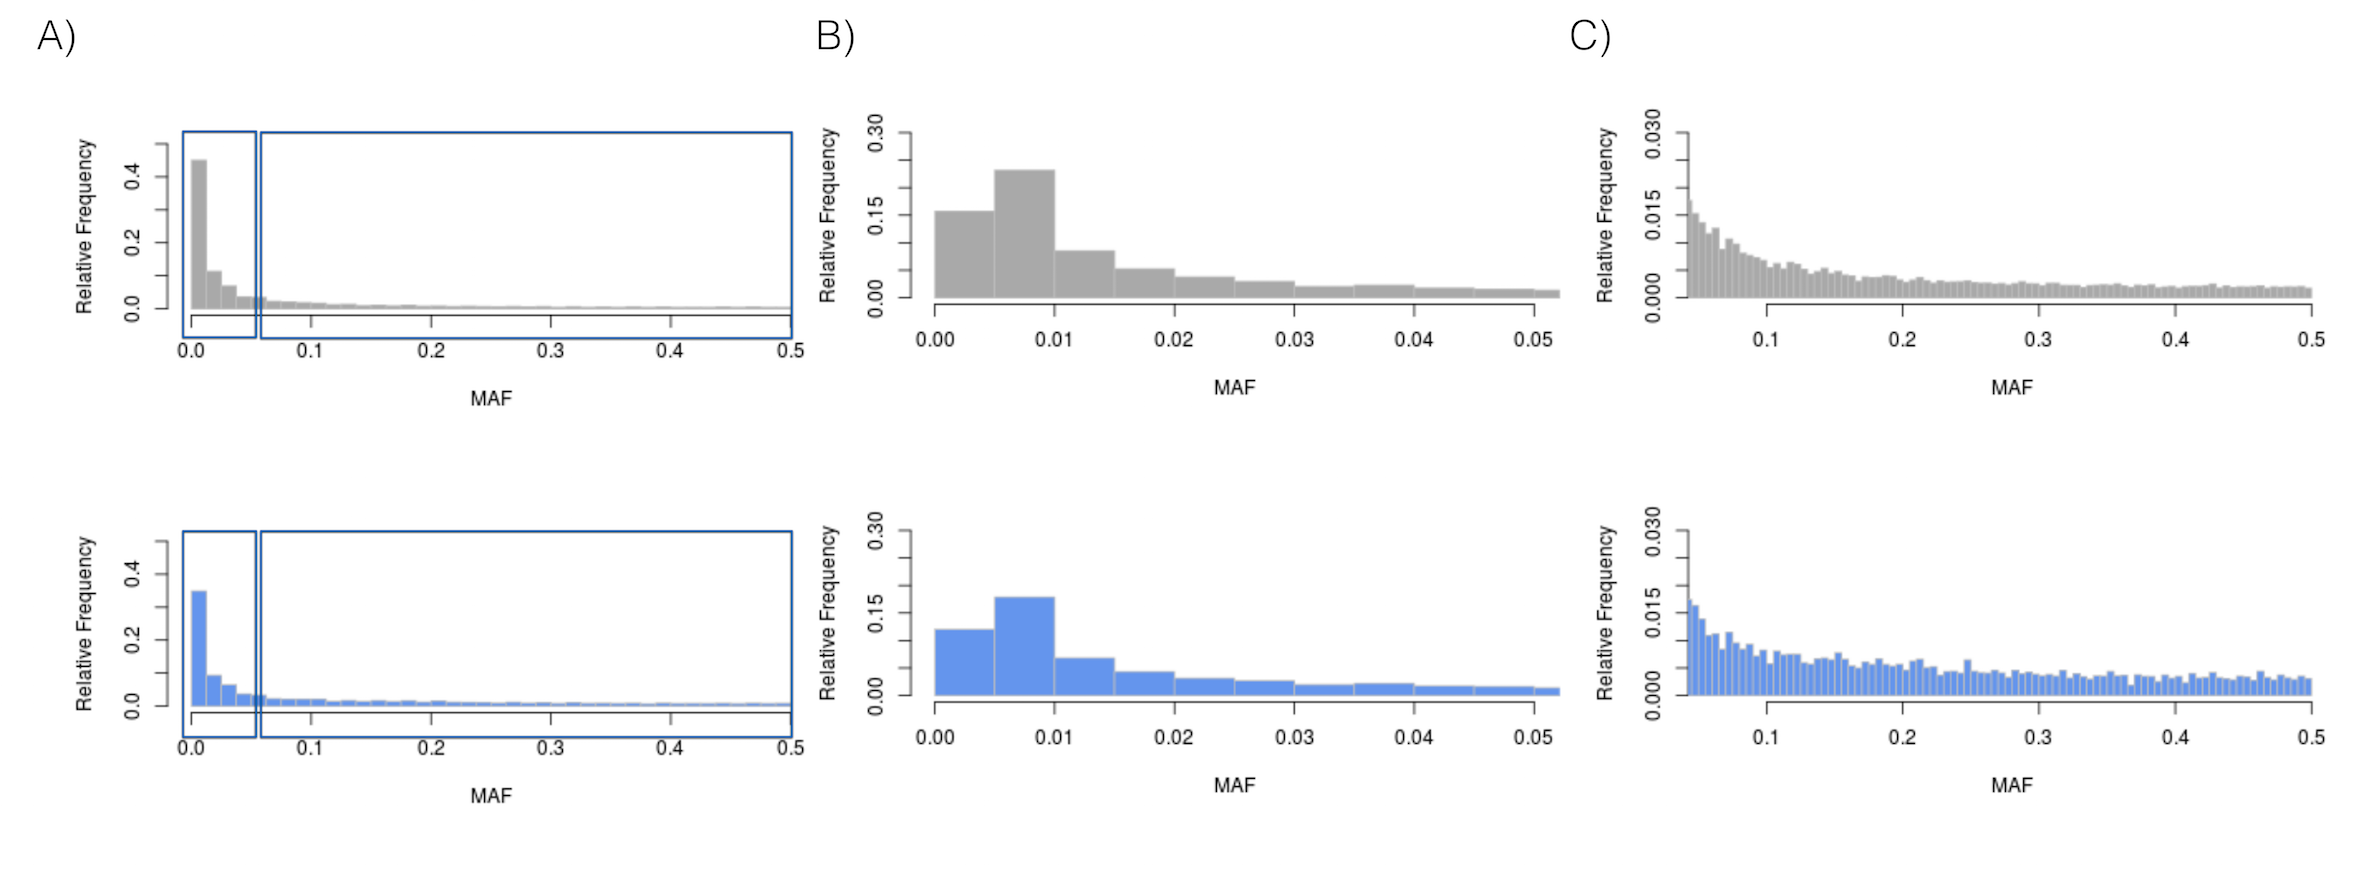
\includegraphics[width= 20 cm, keepaspectratio]
{chap3_folder/figures/SFS_chap2.png}
\caption{\textbf{Site frequency spectrum for protein-coding ($N+S$) SNPs} SNPs come from balanced (blue) and control genes (gray). Rectangles identify the sections that are zoomed in in (B) and (C). } 
\label{fig:SFS}
\end{sidewaysfigure}
%%%%%%%% Figure %%%%%%%%%%%
%%%%%%%% Figure %%%%%%%%%%%

% Para o paper: me ocorreu que o SFS vai ficar mais claro se você plotar ele também usando os log transformed frequencies. Isso irá ressaltar a categoria com efeito forte. 
%BDB: concordo, essa figura tem que melhorar, mas vou deixar assim na tese.

The SFS of the balanced genes is shifted towards intermediate frequencies when compared to the genomic background distribution (Figure ~\ref{fig:SFS}). Specifically, balanced genes have about 10\% less variants in the lower bins of frequency (MAF $\leq 0.0025$). In other words, the balanced genes have a different SFS from that of the background, and an appropriate re-sampling of control SNPs needs to account for this property of the balanced genes. 

The SNPs in the balanced genes were binned according to their MAFs (Table ~\ref{tab:logMAF_bins}), and their distribution into the bins was used for the re-sampling procedure for the controls. Because signatures of LTBS are expected to be restricted to narrow windows (\cite{Andres2009,Andres2011,Bitarello2016,Charlesworth2006}) and here we consider the entire gene, this shift towards intermediate frequencies is modest.

%%%%%%%%%%%%%%%%%%%%%%%%%%%%%%%%%%%%
% this table needs to be completed %
%%%%%%%%%%%%%%%%%%%%%%%%%%%%%%%%%%%%
\begin{sidewaystable}[]
\centering
\scriptsize
\begin{tabular}{@{}ccllclcllllllllllll@{}}
\toprule
\multicolumn{19}{c}{Bins} \\ \midrule
\rowcolor[HTML]{C0C0C0} 
{\color[HTML]{000000} Pop} & \multicolumn{2}{c}{\cellcolor[HTML]{C0C0C0}{\color[HTML]{000000} 1}} & \multicolumn{2}{l}{\cellcolor[HTML]{C0C0C0}2} & \multicolumn{2}{l}{\cellcolor[HTML]{C0C0C0}3} & \multicolumn{2}{c}{\cellcolor[HTML]{C0C0C0}4} & \multicolumn{2}{c}{\cellcolor[HTML]{C0C0C0}5} & \multicolumn{2}{c}{\cellcolor[HTML]{C0C0C0}6} & \multicolumn{2}{l}{\cellcolor[HTML]{C0C0C0}7} & \multicolumn{2}{l}{\cellcolor[HTML]{C0C0C0}8} & \multicolumn{2}{l}{\cellcolor[HTML]{C0C0C0}9} \\ \cmidrule(r){1-19} 
\multicolumn{1}{l}{} & \multicolumn{1}{l}{n} & MAF & n & \multicolumn{1}{l}{MAF} & n & \multicolumn{1}{l}{MAF} & n & MAF & n & MAF & n & MAF & n & MAF & n & MAF & n & MAF \\ \cmidrule(r){2-19}
YRI & 905 & 0.5-0.5 & 277 & 0.9-0.9 & 317 & 1.4-1.8 & 348 & 2.3-3.7 & 292 & 4.2-6.9 & 320 & 7.4-12.5 & 361 & 13-22.2 & 416 &  22.7- 39.3 & 187 & 39.8-50 \\
LWK & 977 & 0.5-0.5 & 386 & 1-1 & 355 & 1.5-2 & 283 & 2.5-3.5 & 335 & 4-7 & 282 & 7.6-12.1 & 390 & 12.6-22.2 & 383 & 22.7-39.4 & 196 & 40-50 \\
MSL & 894 & 0.6-0.6 & 304 & 1.12-1.2 & 208 & 1.8-1.8 & 333 & 2.3-3.5 & 364 & 4.1-7 & 309 & 7.6-12.3 & 390 & 12.9-22.3 & 390 & 22.9-39.4 & 195 & 40-50 \\
GWD & 974 & 0.4-0.4 & 304 & 0.9-0.9 & 395 & 1.3-2.2 & 269 & 2.6-3.5  & 322 & 4-6.6 & 311 & 7.1-12.4 & 368 & 12.8-22.1 & 404 & 22.6-39.4 & 203 & 39.8-50 \\
ESN & 790 & 0.5-0.5 & 303 & 1-1 & 306 & 1.5-2 & 268 & 2.5-3.5 & 334 & 4-7.1 & 300 & 7.6-12.1 & 372 & 12.6-22.2 & 388 & 22.7-39.4 & 200 & 39.9-50 \\
TSI & 820 & 0.5-0.5 & 173 & 0.9-0.9 & 167 & 1.4-1.9 & 175 & 2.3-3.7 & 171 & 4.2-7 & 177 & 7.5-12.1 & 329 & 12.6-22 & 390 & 22.4-39.7 & 194 & 40.2-50 \\
GBR & 586 & 0.55-0.55 & 162 & 1.1-1.1 & 150 & 1.6-2.2 & 145 & 2.7-3.8 & 157 & 4.4-6.6 & 194 & 7.1-12.1 & 313 & 12.6-22 & 363 & 22.5-39.6 & 229 & 40.1-50 \\
FIN & 409 & 0.5-0.5 & 143 & 1-1 & 171 & 1.5-2 & 153 & 2.5-3.5 & 196 & 4-7 & 203 & 7.6-12.1 & 304 & 12.6-22.2 & 370 & 22.7-39.4 & 304 & 39.9-50 \\
CEU & 644 & 0.5-0.5 & 147 & 1-1 & 138 & 1.5-2 & 160 & 2.5-3.5 & 194 & 4-7.1 & 165 & 7.6-12.1 & 325 & 12.6-22.2 & 376 & 22.7-39.4 & 204 & 39.9-50 \\
IBS & 825 & 0.5-0.5 & 173 & 0.9-0.9 & 176 & 1.4-1.8 & 158 & 2.3-3.7 & 191 & 4.2-7 & 176 & 7.5-12.1 & 311 & 12.6-22 & 392 & 22.4-39.7 & 210 & 40.2-50  \\ \bottomrule
\end{tabular}
\caption{\textbf{Binning of SNPs according to their minor allelic frequencies}\\ SNPs in balanced genes were binned according to their logMAF values (see Methods). Values  correspond to the set of balanced genes with HLA SNPs included. When HLA SNPs were excluded, the bin proportions changed (not shown). n, number of SNPs ($N+S$) in the bin; MAF, minimum and maximum MAF values observed within the bin. MAFs are given in \%.}
\label{tab:logMAF_bins}
\end{sidewaystable}

\afterpage{\FloatBarrier}
%%%%%%%%%%%%%%%%%%%%%%%%%%%%%%%%%%%%%%%%%%%%%%%%%%%%%%%%%%%%%%%%%%%%%%%%%%%%%%%%%%%%%
\subsection{Measures of deleteriousness correlate negatively with allelic frequency}
%%%%%%%%%%%%%%%%%%%%%%%%%%%%%%%%%%%%%%%%%%%%%%%%%%%%%%%%%%%%%%%%%%%%%%%%%%%%%%%%%%%%%

Previously, \textcite{Lohmueller2008} reported that SNPs classified as "damaging" according to PolyPhen had significantly lower mean derived allele frequencies (DAF) than "benign" SNPs, with the "probably damaging" category having the lowest mean DAF.

More generally, nonsynonymous variants are expected to have lower frequencies (\cite{Brandvain2016}), because purifying selection will have had enough time to purge deleterious variants from the population (assuming most nonsynonymous variants are deleterious). This is in fact the pattern seen for human populations, where there is a vast excess of low frequency nonsynonymous variants (\cite{Casals2013,Fu2012,Tennessen2012}). Moreover, C scores also tend to be higher for lower frequency variants (\cite{Kircher2014}), although it has been shown that C score distributions have power to differentiate lead-SNPs and tag-SNPs from GWAS, which by definition have similar frequencies (\cite{Kircher2014}).


We confirmed these patterns with the 1000 Genomes data we analyzed (Figure ~\ref{fig:logMAF_bins_2}). When dividing all protein-coding  SNPs (whether they fall into balanced genes or not) into bins of minor allele frequencies (logMAF, see Methods), a clear negative correlation is observed between MAF and the three statistics: $P_{N}/P_{S}$, $P_{del}/P_{S}$ and Cscore (Figure ~\ref{fig:logMAF_bins_2}).

All of the aforementioned observations indicate the importance of controlling for allele frequencies when analyzing the load of deleterious mutations among balanced genes. Lack of a control would cause higher load among control SNPs than for the SNPs from balanced genes, as a consequence of an enrichment in intermediate frequency variants in balanced genes (\cite{Bitarello2016}) and the fact that deleterious variants are more abundant in the lower bins of MAF (\cite{Adzhubei2010,Kircher2014,Lohmueller2008,Subramanian2016}).


%%%%%% Figure %%%%%%% Figure %%%%%%% Figure %%%%%%%%%%%
%%%%%% Figure %%%%%%% Figure %%%%%%% Figure %%%%%%%%%%%
\newpage
\begin{sidewaysfigure}[h]
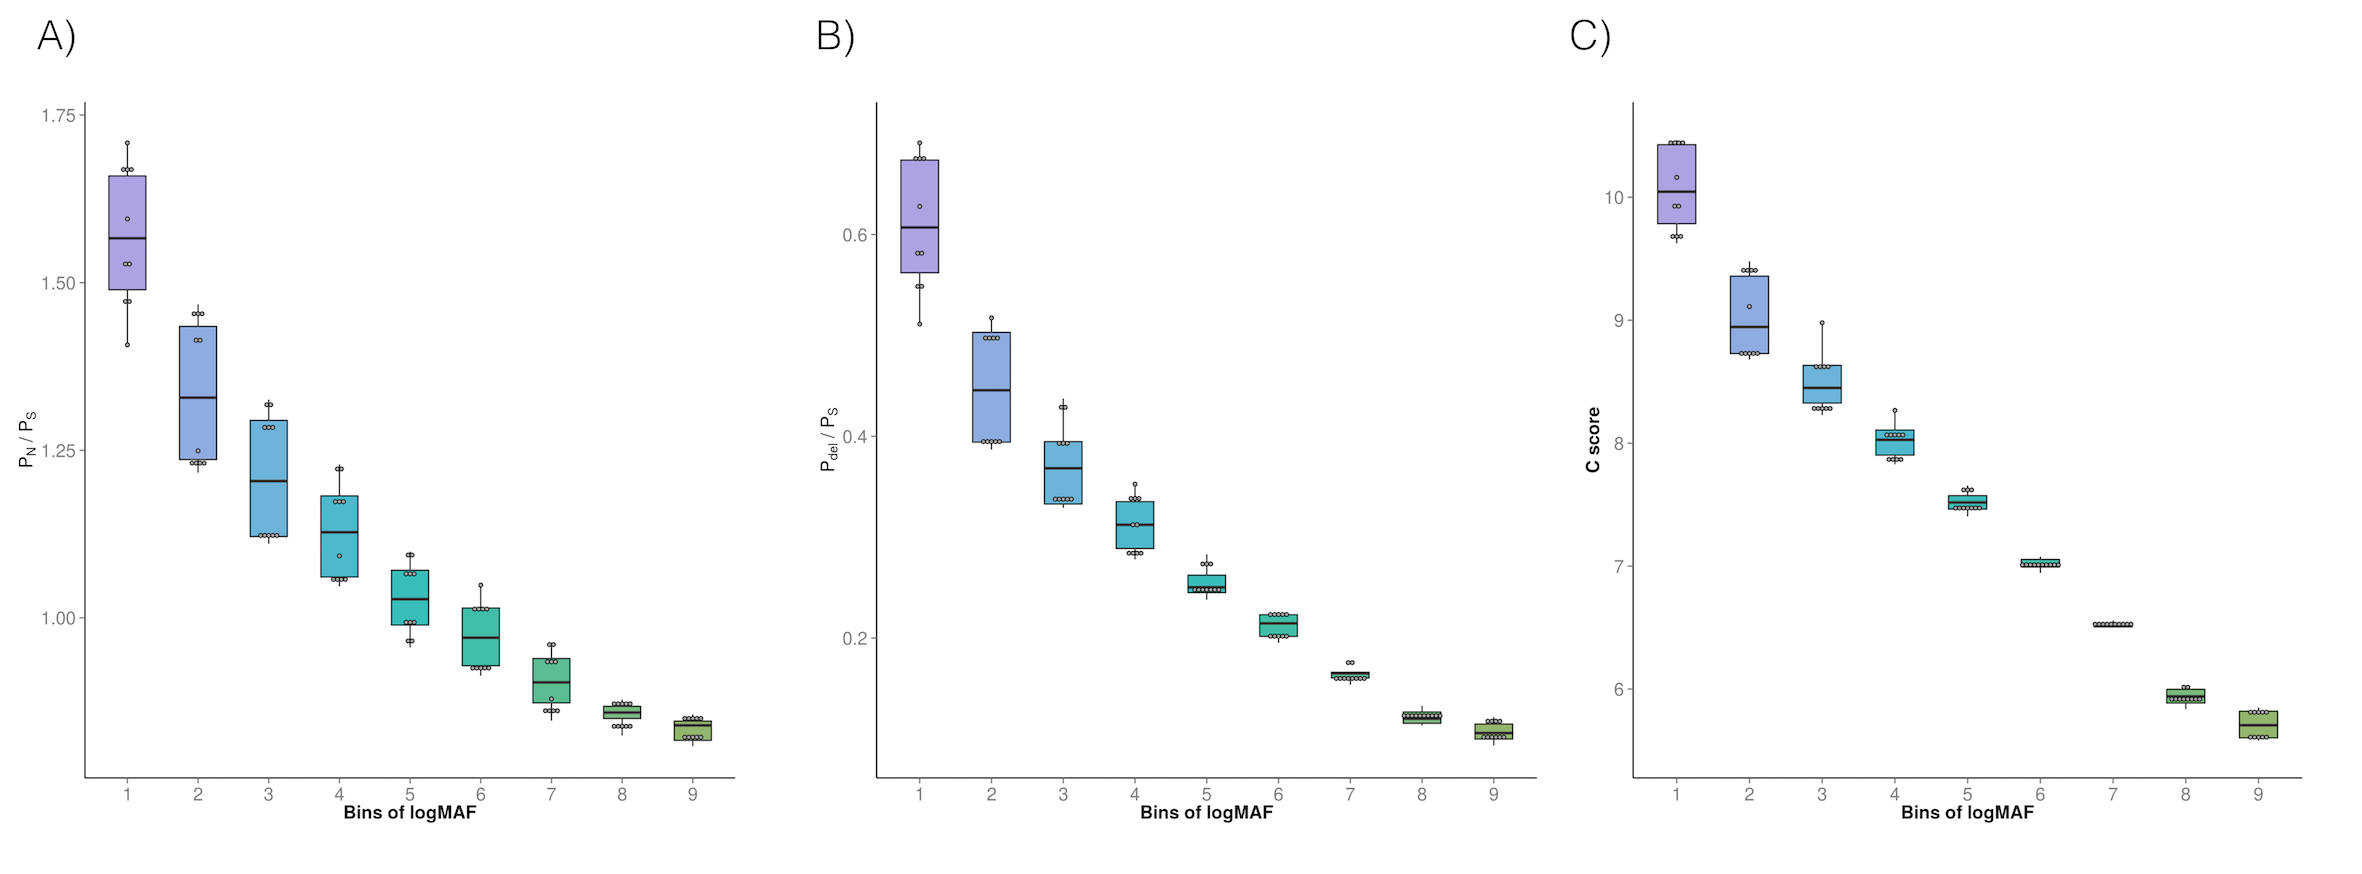
\includegraphics[]{chap3_folder/figures/logMAF_bins_2.png}
\caption{\textbf{Boxplot of load statistics by each bin of MAF.}
All autosomic $N+S$ SNPs were included here. Bins were defined based of the log(base 10) of the MAF of each variant (see Methods).
y-axis, (A) $P_{N}/P_{S}$, (B) $P_{del}/P_{S}$, (C) Cscore.
}
\label{fig:logMAF_bins_2}
\end{sidewaysfigure}

%%% Figure %%%%%%% Figure %%%%
%%% Figure %%%%%%% Figure %%%%



%%% Figure %%%%%%% Figure %%%%
%%% Figure %%%%%%% Figure %%%%
\begin{sidewaysfigure}[h]
\centering
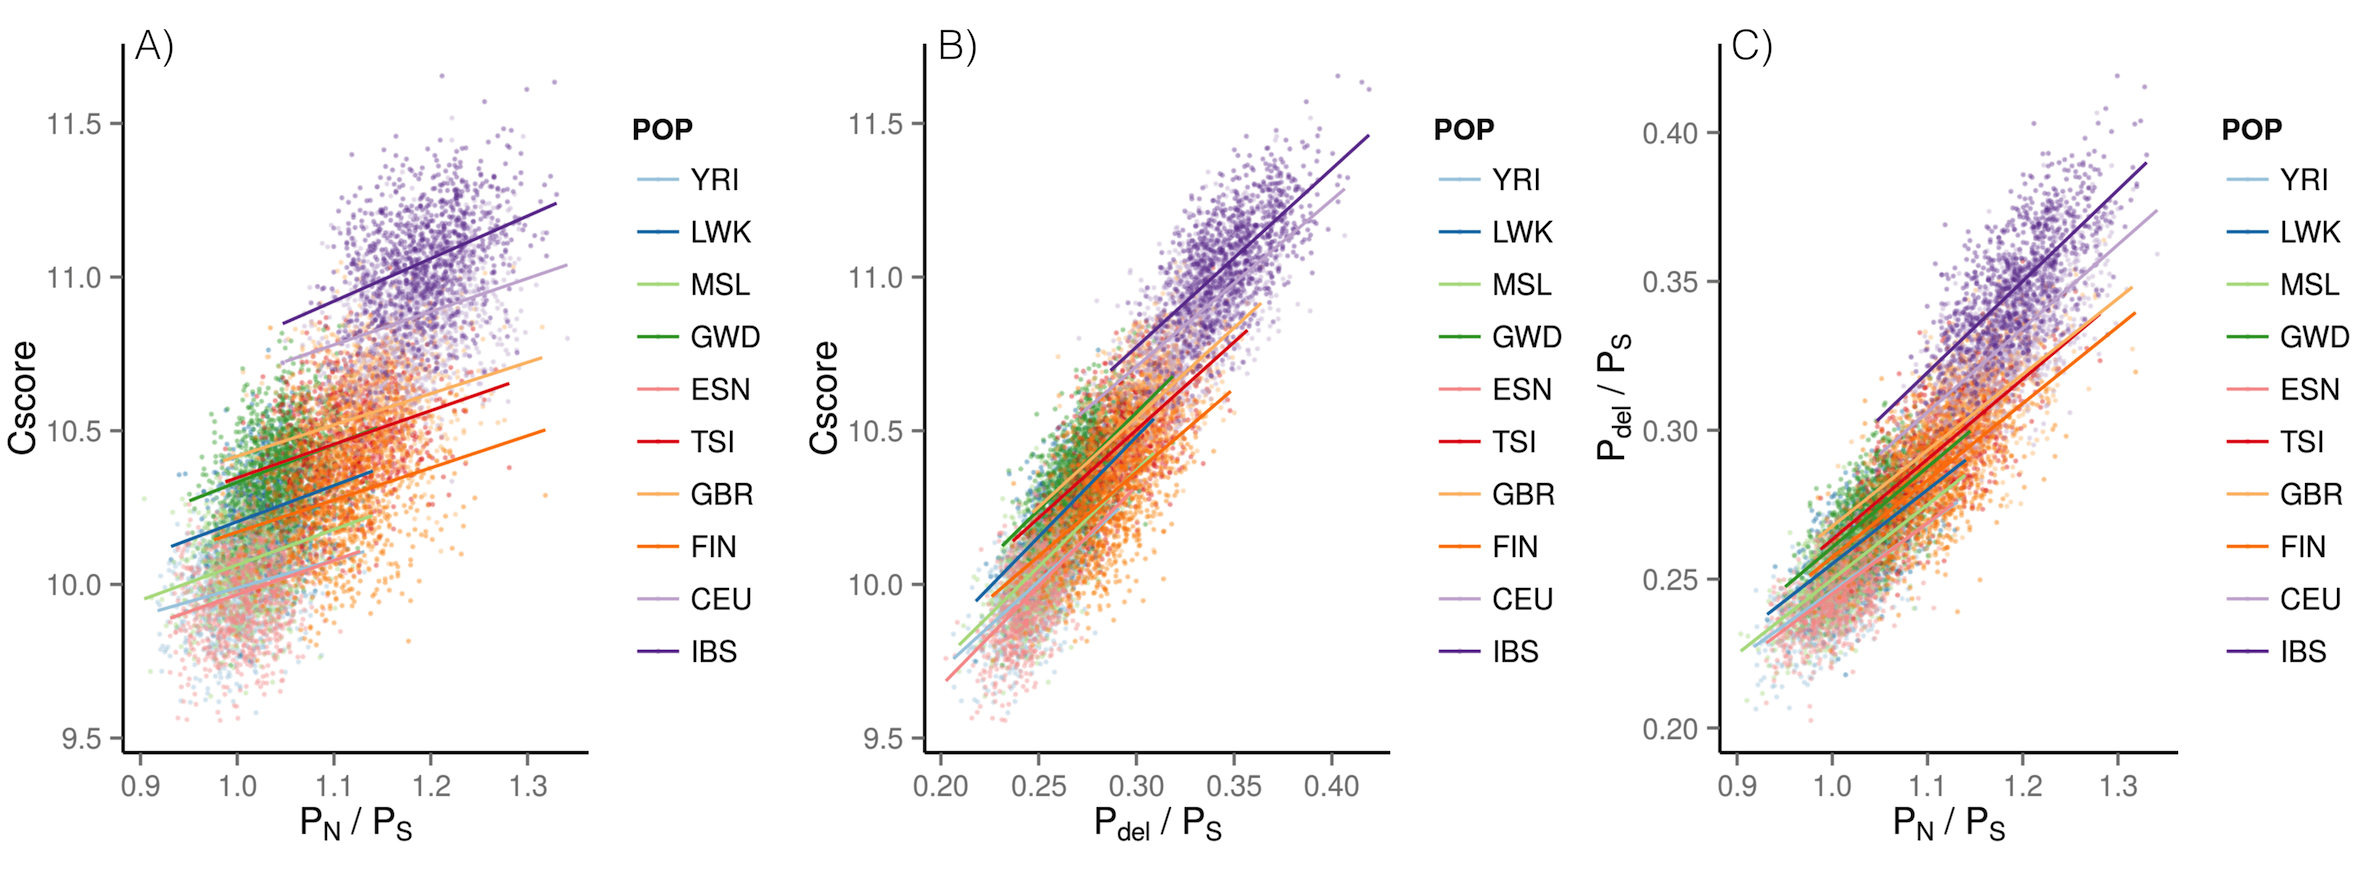
\includegraphics[]{chap3_folder/figures/scatter_del_controls.png}
\caption{\textbf{Correlations between load summary statistics.} (A) C score and $P_{N}/P_{S}$ (cor=0.80, for all populations combined, Pearson, p-value $< 2.2^{e-16}$), (B) $P_{del}/P_{S}$ and Cscore (cor=0.91, $p< 2.2e^{-16}$) and (c) $P_{del}/P_{S}$ and $P_{N}/P_{S}$ (cor=0.91, $p< 2.2e^{-16}$). Each color corresponds to one population and each point is refers to the metric estimated for a re-sampled set of SNPs. Lines represent linear regressions for each population. For correlation values per population, see Table ~\ref{tab:correlations}.}

\label{fig:scatter}
\end{sidewaysfigure}
%%% Figure %%%%%%% Figure %%%%
%%% Figure %%%%%%% Figure %%%%

%%% Table %%% Table %%% Table %%% Table %%% Table %%% Table 
%%% Table %%% Table %%% Table %%% Table %%% Table %%% Table 
%%% Table %%% Table %%% Table %%% Table %%% Table %%% Table 


\begin{table}[h]
\centering
\begin{tabular}{@{}cccc@{}}
\toprule
\rowcolor[HTML]{C0C0C0} 
{\color[HTML]{000000} Pop} & {\color[HTML]{000000} $P_{N}/P_{S}$-Cscore} & {\color[HTML]{000000} $P_{del}/P_{S}$-Cscore} & {\color[HTML]{000000} $P_{N}/P_{S}$-$P_{del}/P_{S}$} \\ \midrule
YRI & 0.23 & 0.55 & 0.61\\
LWK & 0.27 & 0.61 & 0.62 \\
MSL & 0.28 & 0.59 & 0.65 \\
GWD & 0.28 & 0.61 & 0.65 \\
ESN & 0.26 & 0.58 & 0.63 \\
TSI & 0.28 & 0.60 & 0.67 \\
GBR & 0.27 & 0.60 & 0.65 \\
FIN & 0.27 & 0.56 & 0.65 \\
CEU & 0.28 & 0.59 & 0.68 \\
IBS & 0.36 & 0.67 & 0.70 \\ \bottomrule
\end{tabular}
\caption{\textbf{Pearson's correlations between load statistics.} Each value corresponds to 1,000 re-samplings (controls) for the balanced SNPs (gene-based). All correlations are highly significant ($p-value < 2.6e^{-13}$).
}
\label{tab:correlations}
\end{table}
%%%%%%%%%%%%%%%%%%%%%%%%%%%%%%%%%%%%%%%%%%%%%%%
%%%%%%%%%%%%%%%%%%%%%%%%%%%%%%%%%%%%%%%%%%%%%%%


Although our three measures of deleteriousness differ in the criteria used to define/quantify how damaging variants are, we find an overall high correlation among these measures (Figure ~\ref{fig:scatter}). $P_{N}/P_{S}$ and $P_{del}/P_{S}$ are highly correlated in all populations (cor$>0.61$ and $p<2.6e^{-13}$, Table ~\ref{tab:correlations}), and Cscore and $P_{del}/P_{S}$ as well (cor$>0.55$, Table ~\ref{tab:correlations}). $P_{N}/P_{S}$ and Cscore have a weaker correlation, albeit also highly significant (Figure ~\ref{fig:scatter}A and Table ~\ref{tab:correlations}).

These results indicate the importance of using a re-sampling approach that controls for differences in frequencies of SNPs in balanced genes and genomewide (Table ~\ref{tab:logMAF_bins}). Re-sampling sets of genes which are not under balancing selection, without controlling for the SFS, would lead the control to be relatively enriched for low frequency variants, a factor which would obscure the identification of possible differences between the balanced and control SNPs.


\afterpage{\FloatBarrier}
%%%%%%%%%%%%%%%%%%%%%%%%%%%%%%%%%%%%%%%%%%%%%%%%%%%%%%%%%%%%
\afterpage{\clearpage}
\subsection{Extreme values for HLA SNPs} 
%%%%%%%%%%%%%%%%%%%%%%%%%%%%%%%%%%%%%%%%%%%%%%%%%%%%%%%%%%%%

In the scan for balancing selection of \textcite{Bitarello2016}, HLA genes were over-represented among the category of selected genes, and showed extremely strong evidence for selection, with 12 classical HLA genes present among the 213 genes with strongest signatures of balancing selection. This observation, associated to the fact that HLA genes are likely to carry several sites under the direct effects of balancing selection, led us to single them out for an exploratory analysis. %do we need ref for HLA here?

We initially compared the load statistics for the set of SNPs from balanced genes to a group comprising all control SNPs in the genome. Note that here there was no re-sampling involved; we simply compared the statistics between the different groups. We evaluated the influence of SNPs from HLA genes on the load summary statistics by excluding all HLA SNPs from the set of SNPs contained in balanced genes.

The set of SNPs from the balanced genes have different values for the three statistics when compared to the control set of SNPs: $P_{N}/P_{S}$ values are higher (Figure ~\ref{fig:logMAF_bins}), while $P_{del}/P_{S}$ and C score values are lower for the SNPs from all balanced genes (Figure ~\ref{fig:logMAF_bins}). Interestingly, the HLA set of SNPs follows the same pattern as the SNPs from the set of all balanced genes  (which include the HLA SNPs), although in a much stronger way. When we examine HLA genes alone, we find that the average  $P_{N}/P_{S}$ for these loci is almost 2-fold greater than that of control SNPs (Figure ~\ref{fig:logMAF_bins}). Similarly, the reduction in $P_{del}/P_{S}$ and C score in HLA compared to control SNPs is also about two-fold (Figure ~\ref{fig:logMAF_bins}). Moreover, when HLA SNPs are removed from the set of SNPs from balanced genes, the remaining set tends to have values closer to controls, albeit still different (Figure ~\ref{fig:logMAF_bins}).

The extreme patterns of HLA SNPs for these three statistics could be driving the patterns seen in the SNPs from balanced genes, of which they are part of. The $P_{N}/P_{S}$ result is conservative in the sense that, although one could expect lower values for HLA genes (less low frequency and thus less nonsynonymous variants), it is actually almost two-fold higher (Figure ~\ref{fig:logMAF_bins}). This observation likely results from the   high number of sites that are actively maintained by balancing selection in these genes. It is a well-known fact that balancing selection has targeted several sites in HLA genes (e.g. \cite{Hughes1988,Yang2002a,Bitarello2015}), which could at least partially explain the patterns observed for $P_{N}/P_{S}$. The mechanisms driving diversity in the other balanced genes, however, remain largely unknown, and it is reasonable to assume that only one (or a few) site(s) has been targeted by balancing selection in a given gene (e.g. in \cite{Leffler2013a} i.e, that the HLA represents the exception, rather than the rule. 

However, there is no obvious biological explanation as to why $P_{del}/P_{S}$ and C scores should be reduced in HLA compared to control SNPs. This suggests that the reason might be related to allelic frequencies. Moreover, the HLA genes are enriched  not only in intermediate frequency alleles (which are less likely to be deleterious) but also in number of polymorphic sites (\cite{Robinson2013}). Thus, although  HLA genes represent only 12 out of 213 balanced genes considered here, given the high SNP density of the MHC region as a whole, they account for a considerable proportion of the SNPs from balanced genes (Table ~\ref{tab:balancedSNPs}). Thus, in the remaining analyses we estimated load for the set of SNPs from balanced genes with and without the inclusion of HLA SNPs. Because the HLA SNPs change the shape of the SFS, we also re-sampled the control SNPs accordingly.


%%%%%% Figure %%%%%%% Figure %%%%%%% Figure %%%%%%%%%%%
%%%%%% Figure %%%%%%% Figure %%%%%%% Figure %%%%%%%%%%%

\begin{sidewaysfigure}[h]
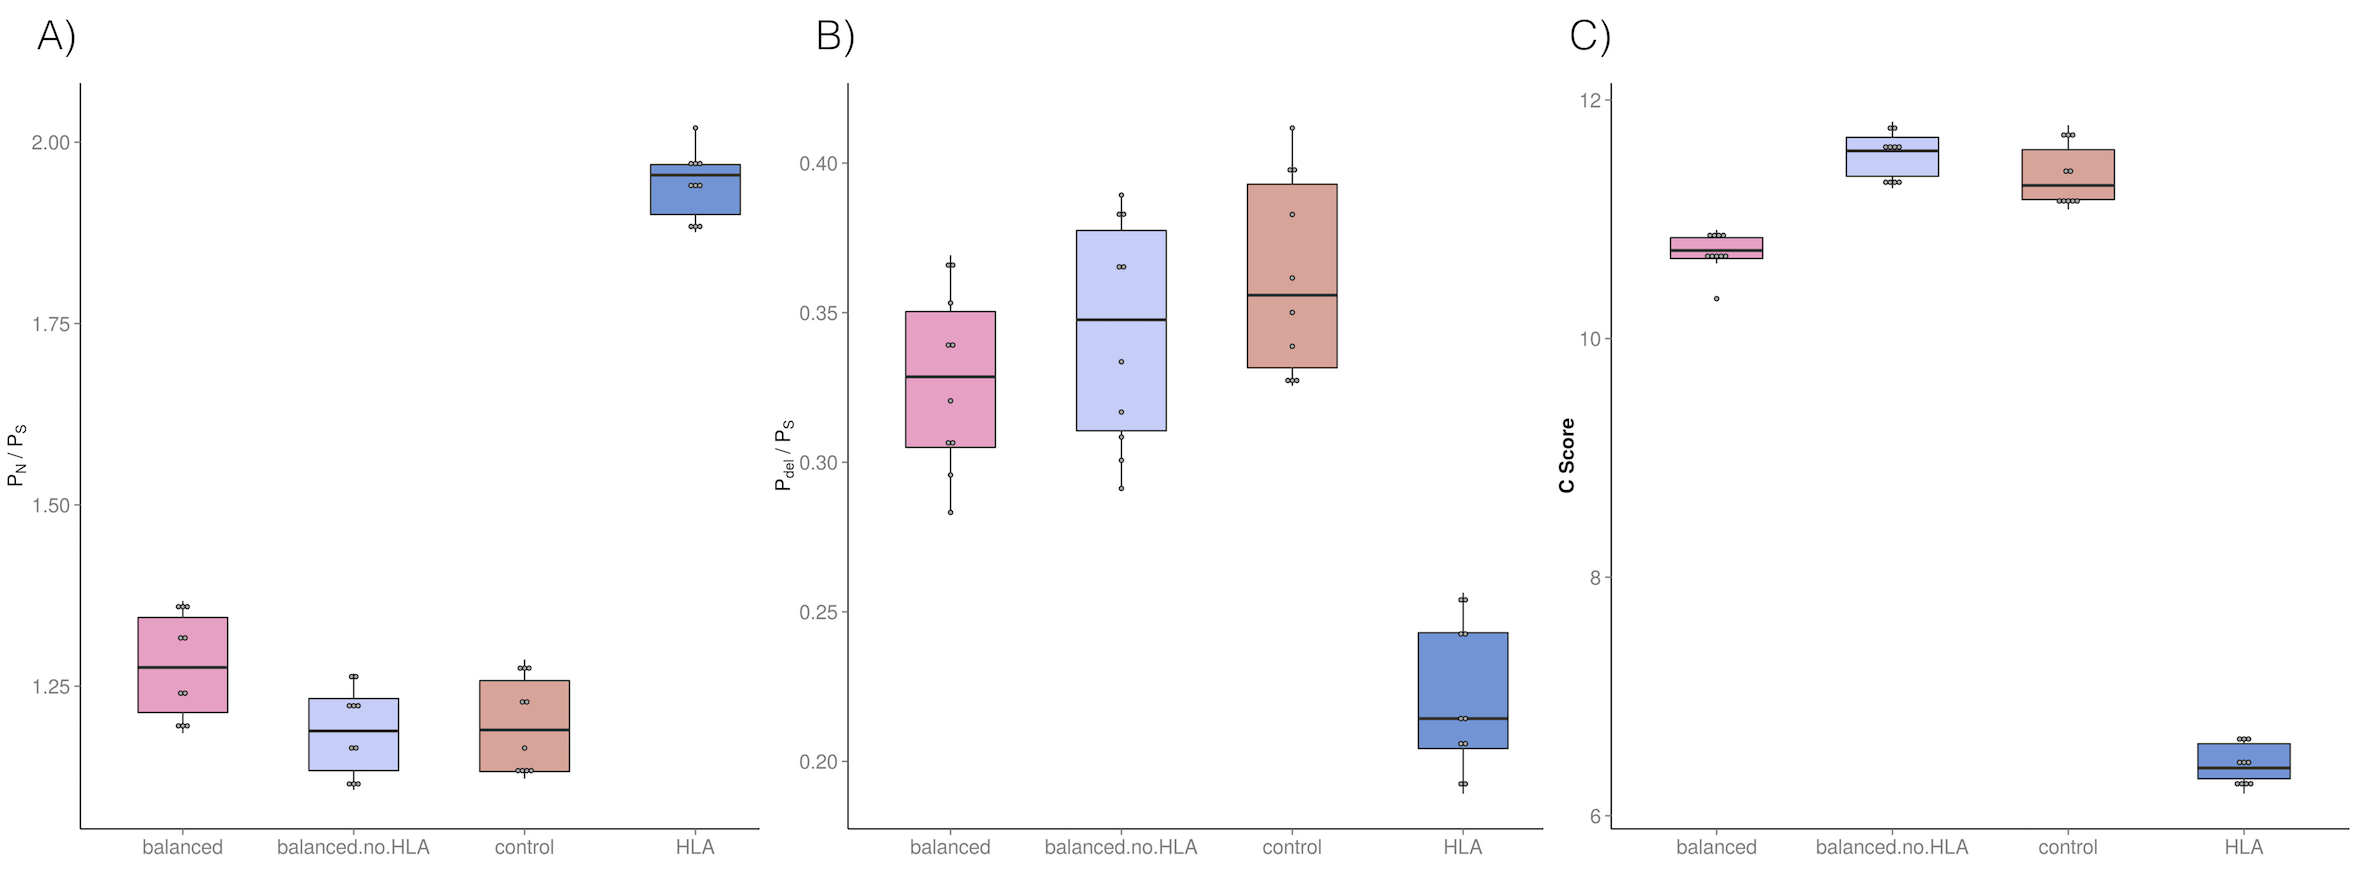
\includegraphics[]{chap3_folder/figures/logMAF_bins.png}
\caption{\textbf{Boxplot of load statistics sets of SNPs.}
Balanced, SNPs contained in the balanced genes; balanced.no.HLA, same as the previous category, but excluding 12 HLA genes (see Methods); control, all SNPs not contained in balanced genes; HLA, a set of 12 HLA genes (see Methods). Each boxplot is composed of 10 data points, each one corresponding to a population (see Methods). y-axis, (A) $P_{N}/P_{S}$, (B) $P_{del}/P_{s}$, (C) Cscore.
}
\label{fig:logMAF_bins}
\end{sidewaysfigure}
%

\afterpage{\FloatBarrier}
%%%%%%%%%%%%%%%%%%%%%%%%%%%%%%%%%%%%%%%%%%%%%%%%%%%%%%%%%%%%%%%%%%%%%%%%%%%%%%%%%%%
\subsection{Increased nonsynonymous to synonymous SNPs in balanced genes}  
%%%%%%%%%%%%%%%%%%%%%%%%%%%%%%%%%%%%%%%%%%%%%%%%%%%%%%%%%%%%%%%%%%%%%%%%%%%%%%%%%%%
Firstly, we note that $P_{N}/P_{S}$ values are on average higher for European than for African populations (Figure ~\ref{fig:PnPs_combo}). This confirms the finding that European populations have a higher proportion of nonsynonymous variants than African populations (\cite{Lohmueller2008}). Since our re-sampling was done by population, we intrinsically take this into account as seen in the control distributions (Figure ~\ref{fig:PnPs_combo}).

The $P_{N}/P_{S}$ values of SNPs from balanced genes are significantly higher than controls ($p<0.01$; Figure ~\ref{fig:PnPs_combo}A). These results are not explained by the HLA genes: although their removal reduces the balanced $P_{N}/P_{S}$ (as expected), while slightly increasing the control values (because the target SFS changes, thus resulting in less intermediate frequencies in the controls), the increase in of balanced genes with respect to the controls remains significant, albeit less extreme (Figure ~\ref{fig:PnPs_combo}B, $P<0.01$ for all African populations and GBR and FIN). One European population has marginally significant values ($P=0.06$, TSI) and for two others (CEU and IBS) $P_{N}/P_{S}$ falls within the control distribution after the removal of HLA SNPs ($P>0.24$, Figure ~\ref{fig:PnPs_combo}B).

The increased $P_{N}/P_{S}$ for balanced genes is also not likely driven by the putative target(s) of balancing selection in these genes: when $P_{N}/P_{S}$ for the balanced genes was estimated after removing the SNP(s) with the highest heterozygosity(ies) for each gene (see Methods), results remain qualitatively similar (Figure ~\ref{fig:PnPs_combo}). In fact, most of the SNPs excluded from the balanced genes were intronic ($\sim 90$\% for all populations, Table ~\ref{tab:Hremove}), and on average 11.5 \emph{N} and 14.6 \emph{S} SNPs were removed from each population (Table ~\ref{tab:Hremove}) which makes the $P_{N}/P_{S}$ estimates increase slightly in most cases (Figure ~\ref{fig:PnPs_combo}). 

These results suggest there is an excess of nonsynonymous variants within the set of balanced genes, and that this excess, at least for African populations, is not entirely explained by the presence of HLA genes (Figure ~\ref{fig:PnPs_combo}B) nor by the presence of a one or a few SNPs per gene that have very high heterozigosities (and are presumably the actual targets of selection). For the European populations the removal of HLA SNPs decreased the estimates in relation to controls in a more pronounced way.

Because nonsynonymous variants are not necessarily deleterious (they might also be neutral), we also investigated two other measures of load that directly quantify deleteriousness.

%%%%%% Figure %%%%%%% Figure %%%%%%% Figure %%%%%%%%%%%
%%%%%% Figure %%%%%%% Figure %%%%%%% Figure %%%%%%%%%%%
\begin{sidewaysfigure}[h]
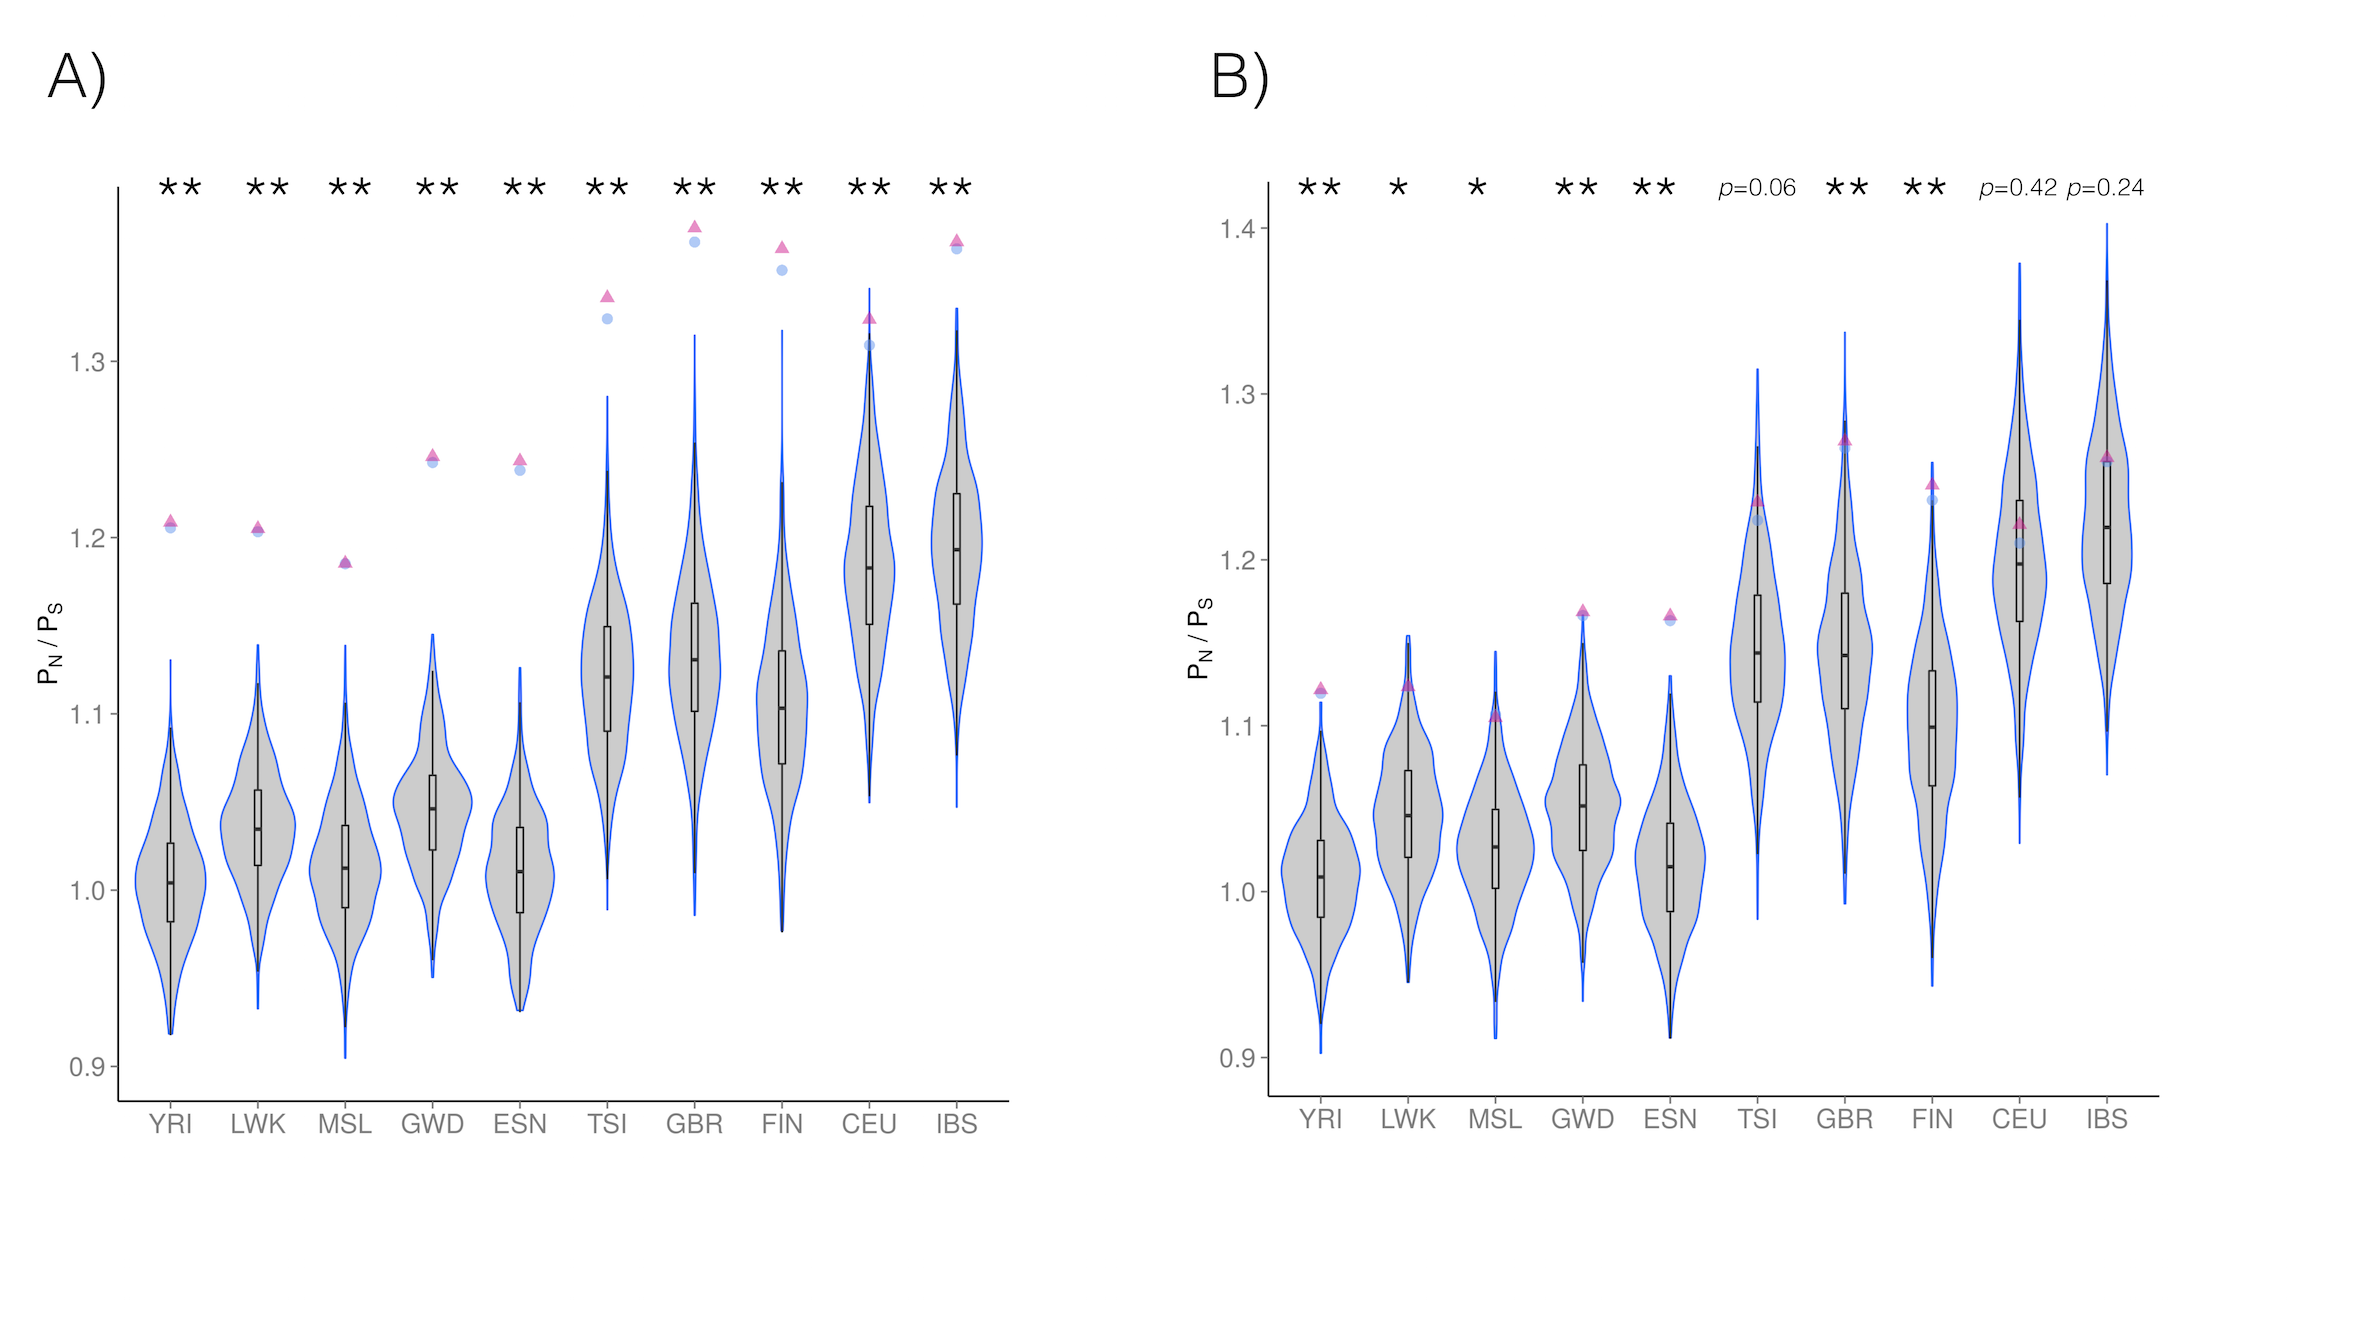
\includegraphics[]{chap3_folder/figures/PnPs_combo2.png}
\caption{\textbf{$P_{N}/P_{S}$ for balanced genes} A) Including HLA SNPs; B) removing HLA SNPs. Blue circle, estimate for all protein-coding SNPs in the set; pink triangle, estimate after removal of SNP(s) with highest heterozygosity in each gene (see Methods. **, $p-value<0.01$, *$p<0.05$. Reported p-values are for the estimates with all SNPs.}
\label{fig:PnPs_combo}
\end{sidewaysfigure}

%%%%%% Figure %%%%%%% Figure %%%%%%% Figure %%%%%%%%%%%
%%%%%% Figure %%%%%%% Figure %%%%%%% Figure %%%%%%%%%%%
%%%%%%%%%%%%%%%%%%%%%%%%%%%%%%%%%%%%%%%%%%%%%%%%%%%%%%%

%%%%%%%%%%%%%%%%%%%%%%%%%%%%%%%%%%%%%%%%%%%%%%%%%%%%%%%%%%%%%%%%%%%%%%%%%%%%%%%%%%%%%%%%%%%%%%%%%%%%%%%%%%%%%%%%%%%%%%
\subsection{Increased proportion of damaging to synonymous SNPs in balanced genes} 
%%%%%%%%%%%%%%%%%%%%%%%%%%%%%%%%%%%%%%%%%%%%%%%%%%%%%%%%%%%%%%%%%%%%%%%%%%%%%%%%%%%%%%%%%%%%%%%%%%%%%%%%%%%%%%%%%%%%%%

Again, we note that European populations have higher balanced and control values than African populations, as seen previously (\cite{Lohmueller2008}). When comparing $P_{del}/P_{S}$ estimates for SNPs from balanced genes and control sets of SNPs, a similar pattern emerges, although less extreme than the one seen for $P_{N}/P_{S}$: balanced genes tend to have higher load compared to controls ($p<0.05$) for all populations, except CEU and IBS ($p>0.14$; Figure ~\ref{fig:PdelPs_combo}A).


The removal of HLA SNPs only slightly changes the $P_{del}/P_{S}$, and the qualitative relationship between them does not change, with all populations except CEU and IBS having $p<0.05$ (Figure ~\ref{fig:PdelPs_combo}). This differs from what was observed for $PN/PS$, where the removal of HLA SNPs made the estimates of load for balanced genes less different from controls, although still highly significant. 

Moreover, the $P_{del}/P_{S}$ estimates with and without the removal of SNPs with the highest heterozygosity per gene  only slightly increase the estimates, compatible with the observation that few of the removed SNPs with this filter are nonsynonymous, and always less than the number of synonymous SNPs (Table ~\ref{tab:Hremove}).

The results for $P_{del}/P_{S}$ are in agreement with what was observed for $P_{N}/P_{S}$, suggesting that the patterns observed for $P_{N}/P_{S}$ are driven by deleterious, and not adaptive or neutral nonsynonymous variants. 

%%%%%% Figure %%%%%%% Figure %%%%%%% Figure %%%%%%%%%%%
%%%%%% Figure %%%%%%% Figure %%%%%%% Figure %%%%%%%%%%%

\begin{sidewaysfigure}[h]
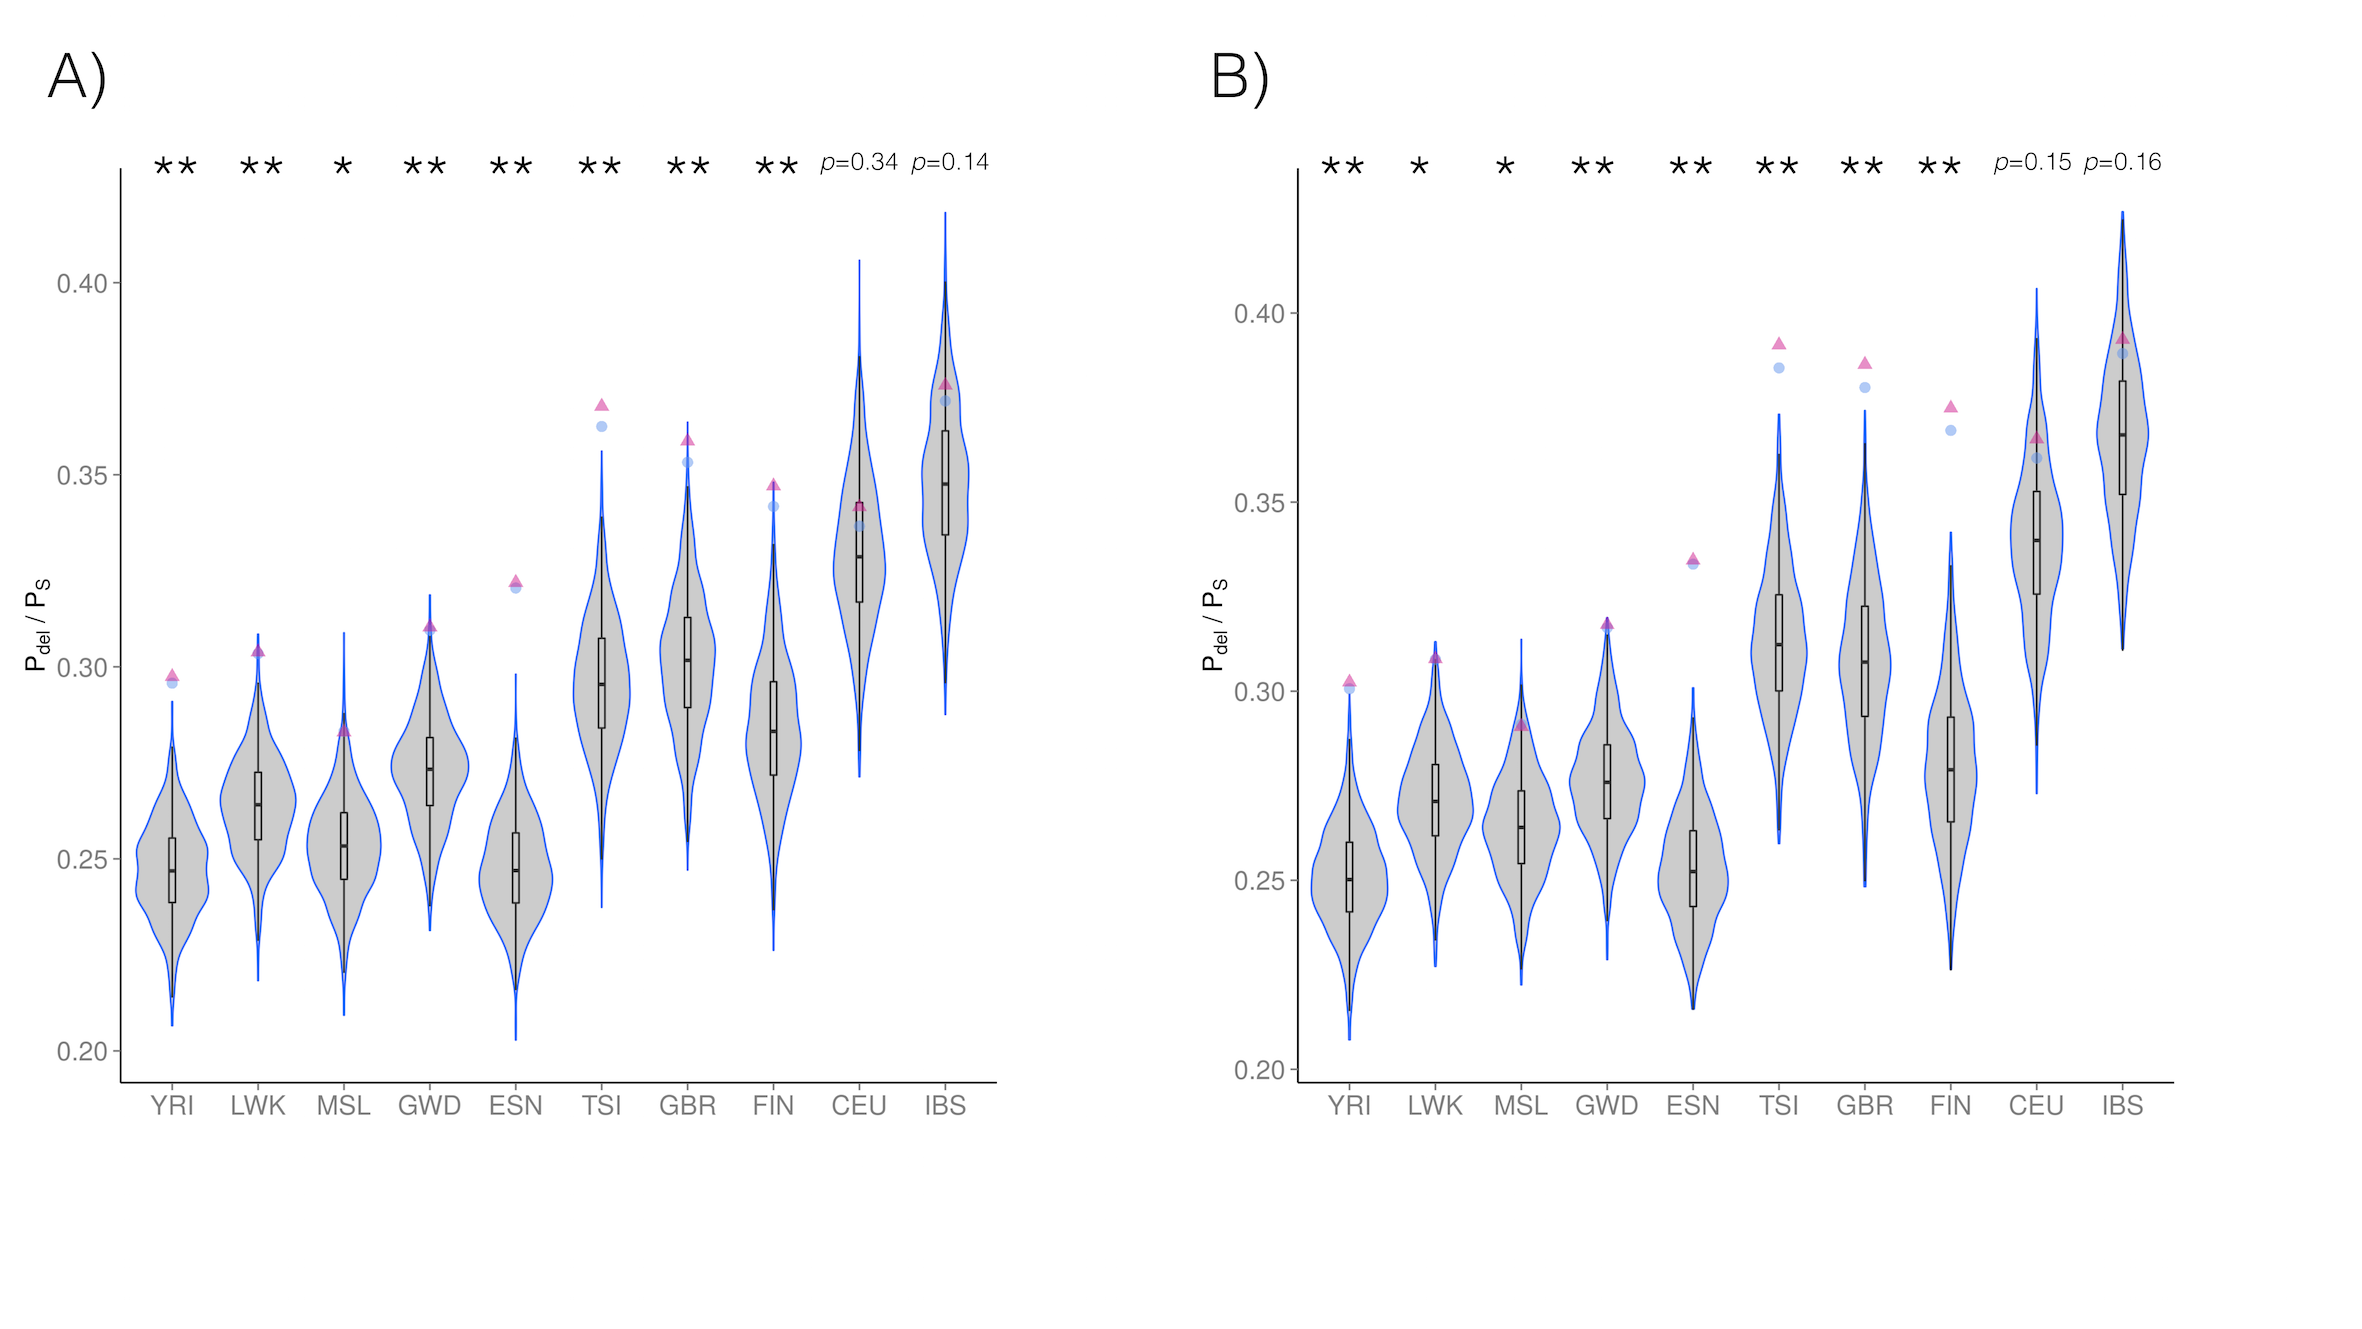
\includegraphics[]{chap3_folder/figures/PdelPs_combo2.png}
\caption{\textbf{$P_{del}/P_{S}$ for balanced genes} A) Including HLA SNPs; B) removing HLA SNPs. Blue circle, estimate for all protein-coding SNPs in the set; pink triangle, estimate after removal of SNP(s) with highest heterozygosity in each gene (see Methods). **, $p<0.01$, *$p<0.05$. Reported p-values are for the estimates with all SNPs.}
\label{fig:PdelPs_combo}
\end{sidewaysfigure}

%%%%%% Figure %%%%%%% Figure %%%%%%% Figure %%%%%%%%%%%
%%%%%% Figure %%%%%%% Figure %%%%%%% Figure %%%%%%%%%%%

\afterpage{\FloatBarrier}
%%%%%%%%%%%%%%%%%%%%%%%%%%%%%%%%%%%%%%%%%%%%%%%%%%%%%%%%%%%%%%%%%%%%%%%%
%%%%%%%%%%%%%%%%%%%%%%%%%%%%%%%%%%%%%%%%%%%%%%%%%%%%%%%%%%%%%%%%%%%%%%%%
\subsection{Increased C-scores in balanced genes} 

Average scaled C scores yield qualitatively different results with respect to analyses based on $P_{N}/P_{S}$ and $P_{del}/P_{S}$. Firstly, for African populations and for TSI the load estimates for balanced genes are very elevated ($p<0.01$) compared to controls, similarly to what was seen for $P_{N}/P_{S}$ (Figure ~\ref{fig:Cscore_combo}A). However, this pattern is not observed for the other European populations, with p-values approaching one for CEU and IBS (Figure ~\ref{fig:Cscore_combo}A). Interestingly, in this case, the removal of HLA SNPs enhances the signal: African values become even more extreme and all the European populations acquire extreme values when compared to controls as well ($p<0.01$ for all populations, Figure ~\ref{fig:Cscore_combo}B).


%%%%%% Figure %%%%%%% Figure %%%%%%% Figure %%%%%%%%%%%
%%%%%% Figure %%%%%%% Figure %%%%%%% Figure %%%%%%%%%%%
\begin{sidewaysfigure}[h]
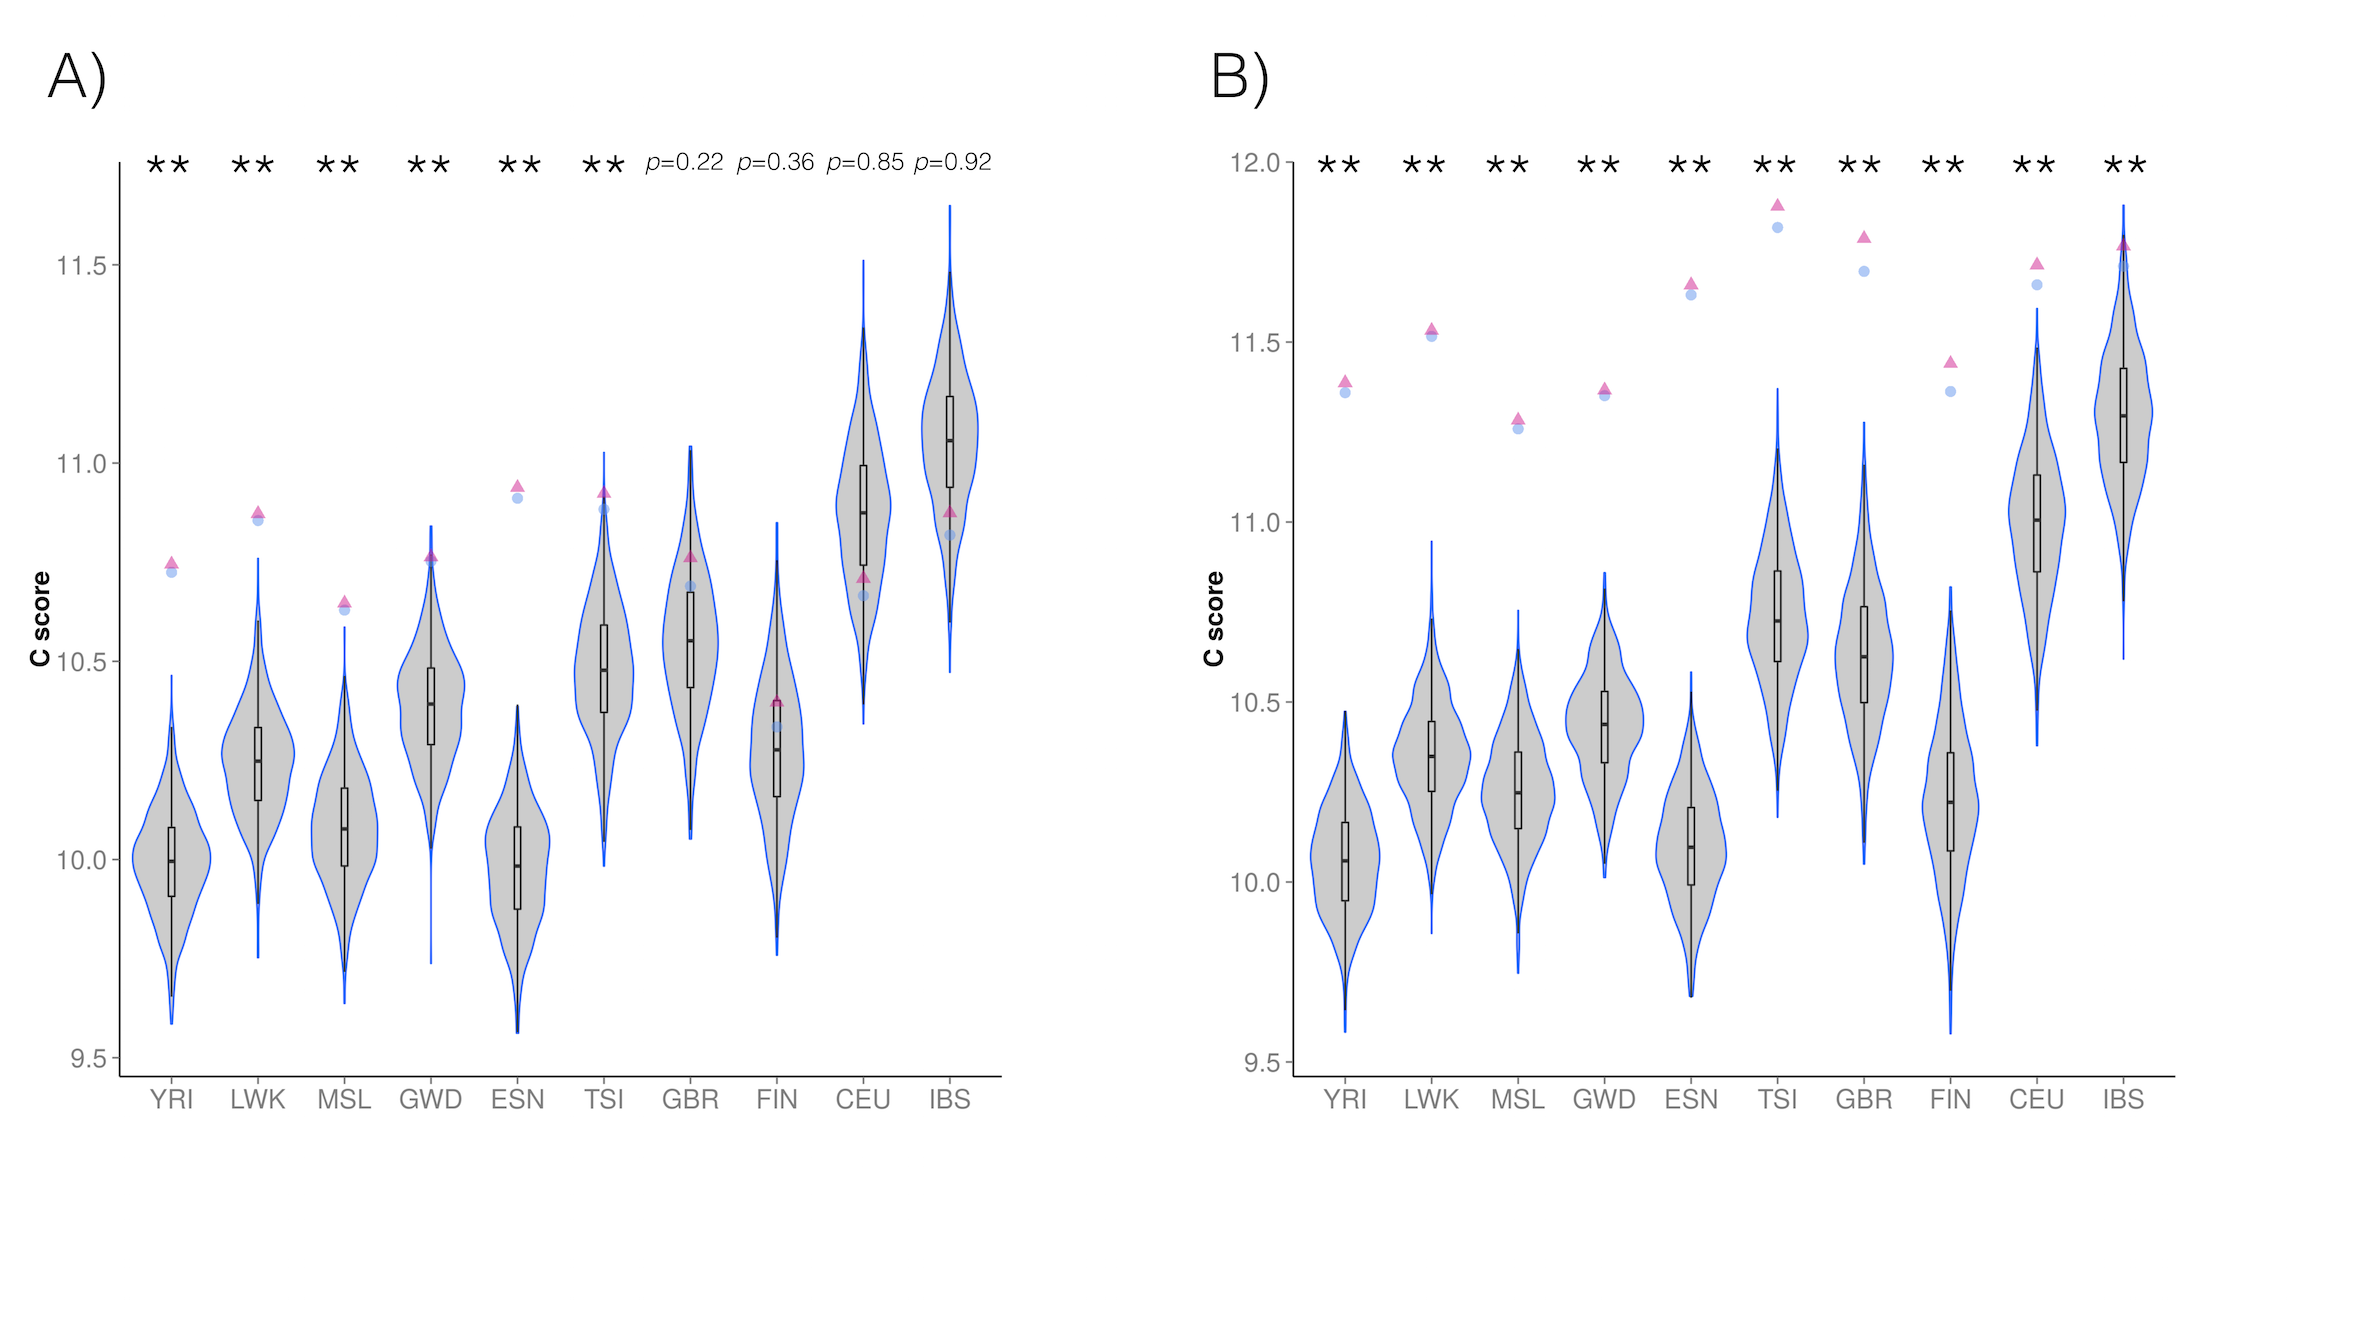
\includegraphics[]{chap3_folder/figures/Cscore_combo2.png}
\caption{\textbf{Average scaled Cscore for balanced genes.} A) Including HLA SNPs; B) removing HLA SNPs. Blue circle, estimate for all protein-coding SNPs in the set; pink triangle, estimate after removal of SNP(s) with highest heterozygosity in each gene (see Methods). **, $p<0.01$, *$p<0.05$. Reported p-values are for the estimates with all SNPs.}
\label{fig:Cscore_combo}
\end{sidewaysfigure}

%%%%%% Figure %%%%%%% Figure %%%%%%% Figure %%%%%%%%%%%
%%%%%% Figure %%%%%%% Figure %%%%%%% Figure %%%%%%%%%%%


Given that the most appropriate set of SNPs for testing our hypothesis of load  is the set without HLA genes and without the SNPs with the highest heterozigosities per gene (Figure ~\ref{fig:Cscore_combo}B), pink triangle), it is plausible that the reduction or loss of significance of the load in the set of all balanced genes (in Africa and Europe, respectively) is due to the excess of adaptive variants (from HLA or other genes) present in the complete set, which tend to have lower C scores. Note that the control distributions in Figures ~\ref{fig:Cscore_combo}A and ~\ref{fig:Cscore_combo}B are very similar, and what changes dramatically is the load estimate for the balanced genes. Also, the Scaled C scores are PHRED-scaled, ranging from 1 to 99, with the top 10\% most deleterious variants having scores above 10, and the top 1\% above 20, and so on (\cite{Kircher2014}). Thus this difference is likely to be even greater than what is conveyed by this analysis.


We also looked at the raw C scores which provide more power in tests comparing sets of SNPs (\cite{Kircher2014}). For African populations, balanced genes have raw C score distributions with significantly higher values than the controls (Mann-Whitney U test, one-tailed, P<=0.05) for more than 70\% of the control re-samplings (Table ~\ref{tab:rawC}), except for GWD, for which only 251 out of 1,000 controls  have significantly lower C scores than the balanced genes. For Europe, only TSI has 13\% of the controls with lower C scores than the balanced genes, and all other populations have less than 5 such cases (Table ~\ref{tab:rawC}). 

%%%%%%%%% table %%%%%%% table %%%%%%%%%
%%%%%%%%% table %%%%%%% table %%%%%%%%%
\begin{table}[h]
\centering
\begin{tabular}{@{}ccc@{}}
\toprule
\rowcolor[HTML]{C0C0C0} 
{\color[HTML]{000000} Pop} & {\color[HTML]{000000} HLA included} & HLA excluded \\ \midrule
 & $P<0.05$ & \multicolumn{1}{c}{$P<0.05$} \\
YRI & 959 &  1,000 \\
LWK & 805 &  1,000 \\
MSL & 727 &  1,000 \\
GWD & 251 &  1,000 \\
ESN & 995 &  1,000 \\
TSI & 130 &  999 \\
GBR & 5 &  995 \\
FIN & 1 &  999 \\
CEU & 0 & 844 \\
IBS & 0 &  1,000\\ \bottomrule
\end{tabular}
\caption{\textbf{Raw C score comparison between balanced genes and controls}
For each comparison, the alternative hypothesis was that balanced genes had higher raw C score values than the control distribution (Mann-Whitney U test, one-tailed). Values refer to the number of comparisons (out of 1,000 control distributions) for which the null hypothesis (distributions are not different) was rejected ($P<0.05$).
}
\label{tab:rawC}
\end{table}
%%%%%%%%% table %%%%%%% table %%%%%%%%%
%%%%%%%%% table %%%%%%% table %%%%%%%%%

However, when we perform the same analyses for the balanced genes after the removal of HLA SNPs, balanced genes have higher raw C scores for all comparisons in African populations, and for more than 995 comparisons for all European populations, except CEU, for which 844 comparisons are significant (Table ~\ref{tab:rawC}).


%%%%%%%%%%%%%%%%%%%%%%%%%%%%%%%%%%%%%%%%%%%%%%%%%%%%%%%%%%%%%%%%%%%%%%%%%%%%%%%%%%%%%%%%%%%%%%%%%%%%%%%%%%%%%%%%%%%%%%%%%%%%%%%%%%%%%%%%%%%%%%%%
%%%%%%%%%%%%%%%%%%%%%%%%%%%%%%%%%%%%%%%%%%%%%%%%%%%%%%%%%%%%%%%%%%%%%%%%%%%%%%%%%%%%%%%%%%%%%%%%%%%%%%%%%%%%%%%%%%%%%%%%%%%%%%%%%%%%%%%%%%%%%%%%
%%%%%%%%%%%%%%%%%%%%%%%%%%%%%%%%%%%%%%%%%%%%%%%%%%%%%%%%%%%%

\section{Discussion and Conclusions}   %%%%%%%%%%%%%%%%%%%%%
%%%%%%%%%%%%%%%%%%%%%%%%%%%%%%%%%%%%%%%%%%%%%%%%%%%%%%%%%%%%

\subsection{Increased genetic load in balanced genes}

The study of slightly deleterious mutations is one of the pillars of population genetics (\cite{Kondrashov1995}). The fate of mutations is highly dependent on   the effective population size ($N_{e}$) and its relationship to the selection coefficients. As a consequence, weakly deleterious mutations might  reach moderate frequencies in small, but not in large populations, where selection is more effective. Moreover, linkage to selected variants is also a major determinant of the fate of a deleterious mutation (\cite{Hill1966,Cutter2013}).

The fates of strongly deleterious mutations are mostly deterministic in terms of mutation rates and selection coefficients -- i.e, when $s>>1/2N_{e}$ (where $s$ is the selection coefficient). The  fate of very slightly deleterious mutations -- i.e, almost neutral -- is, however, mostly stochastic, driven by genetic drift (\cite{Kondrashov1995}). But what happens when considerably strong selection (positive, negative, balancing) on a site impacts the sites in its vicinity? Here, we examined how balancing selection shapes the accumulation of deleterious mutations in the vicinity of its targets. 

We showed that genes with strong signatures of long-term balancing selection have increased levels of nonsynonymous to synonymous polymorphisms, damaging to synonymous polymorphisms, and also elevated deleteriousness scores (\cite{Kircher2014}), when compared to controls. We took special care in controlling for the fact that balanced genes have a site-frequency spectrum which is different from the genomic background, with proportionally more intermediate frequency variants, and we also accounted for the fact that within the balanced genes there are sites directly under balancing selection, which could be incorrectly assigned to deleterious variants according to some classification methods.

Because HLA genes are known as an example of multi-locus balancing selection -- i.e, several positions within the HLA genes have been targets of selection (\cite{Hughes1988,Yang2002a,Bitarello2015}) -- it seemed plausible that their considerable contribution to the set of balanced genes could be responsible for the overall patterns we observed. Therefore, in all analyses we compared results for balanced genes including and excluding HLA genes. This approach is  conservative, given that not all SNPs in HLA genes are expected to be direct targets of selection. A less drastic solution would be to single out the exons of HLA genes which harbour most -- if not all -- of the balanced polymorphisms in those genes and exclude only the SNPs contained in those exons (\cite{Klein1986}). 

Additionally, we also  removed from each balanced gene the SNP(s) likely to be the targets of balancing selection, in order to filter our datasets from the potentially conflicting patterns generated by advantageous and deleterious variants within the balanced genes. Importantly, in this approach we only excluded the SNP(s) with the highest heterozigosiy among those contained in a window with a very strong signature of LTBS as reported in \textcite{Bitarello2016}, thus increasing the chance that the actual selected site was filtered out.

%%%%%%%%%%%%%%%%%%%%%%%%%%%%%%%%%%%%%%%%%%%%%%%%%%%%%%%%%%%%%%%%%%%%
\subsection{The challenges of quantifying genetic load} 
%%%%%%%%%%%%%%%%%%%%%%%%%%%%%%%%%%%%%%%%%%%%%%%%%%%%%%%%%%%%%%%%%%%%

Establishing the damaging potential of a variant is a formidable task in itself (\cite{Grimm2015}). Quantifying the genetic load and comparing it between groups (populations, SNPs, genes, etc) is also challenging, as demonstrated by the great number of published contrasting results regarding genetic load in humans (reviewed in \cite{Henn2015a}). Therefore, it is important to justify the methodology used here. 

We chose to use statistics based on the counts of deleterious variants ($P_{N}/P_{S}$ and $P_{del}/P_{S}$) and deleteriousness scores (C score). With $P_{N}/P_{S}$ and $P_{del}/P_{S}$ we quantified the proportions of nonsynonymous and potentially damaging variants, respectively, for balanced genes and control groups. $P_{N}$ simply documents whether the  polymorphism changes the coded aminoacid, and thus is unbiased with respect to knowledge of the frequency at which the polymorphism is segregating. Nevertheless, $P_{N}$ counts are composed of neutral, deleterious and advantageous variants and thus are not  straight-forward to interpret. $P_{del}$ is more accurate than $P_{N}$ as a measure of deleteriousness, but it is restricted to  nonsynonymous sites and is only available for a subset of the nonsynonymous variants ($\sim 80$\% for the genome, but $\sim 70$\% for balanced genes), thus reducing its power, particularly in small sets of SNPs. Moreover, PolyPhen-2 has been shown to overfit its training data and not to generalize well for other datasets (\cite{Grimm2015}). Neither of these approaches incorporate the frequency of the deleterious mutations when classifying SNPs.  

One possible frequency-based measure would be the ratio of heterozygosities at nonsynonymous and synonymous sites ( $\pi_{N}/\pi_{S}$ ), but this ratio is particularly sensitive to recent bottlenecks (reviewed in \cite{Brandvain2016}). This is because, after a bottleneck, nonsynonymous variation recovers more quickly than synonymous variation (because there are more nonsynonymous sites), and so an elevated $\pi_{N}/\pi_{S}$  following a bottleneck could be inferred (wrongly) as relaxed  selection. \textcite{Do2015,Simons2014} use and recommend a direct estimate of the number of deleterious (or nonsynonymous) mutations (e.g. $PN/PS$ and $Pdel/PS$), which is robust to violations of demographic equilibrium (reviewed in \cite{Brandvain2016,Henn2015a}). 

Our approach here is thus conservative. Previous studies have shown that for comparisons between African and Out-of-Africa, small or no difference is verified when the number of putative deleterious mutations is counted (\cite{Henn2016,Tennessen2012,Do2015,Lohmueller2014}), whereas on average the out-of-Africa populations are more homozygous for the putative deleterious mutations (\cite{Lohmueller2008}) -- a difference not detectable by these two methods.

In addition to this \enquote{SNP counting} approach, we also compared the distribution of deleteriousness among all SNPs within the balanced genes and controls via the C score (\cite{Kircher2014}) analyses. The C score is defined for all $N+S$ sites and combines desirable features from other annotations, but is also negatively correlated with allelic frequency (as are the other two statistics used here). The C score does not suffer from poor generalization properties like PolyPhen-2, because the vector machine was trained on an independent dataset (\cite{Grimm2015,Kircher2014}). However, CADD (C score) was trained on high frequency variants, and although the C scores are available for all 1000 Genomes Phase 3 variants (\cite{Kircher2014}) its accuracy in differentiating deleteriousness of for low MAF variants is likely to be  smaller.

%%%%%%%%%%%%%%%%%%%%%%%%%%%%%%%%%%%%%%%%%%%%%%%%
\subsection{Sheltered load and hitch-hiking}
%%%%%%%%%%%%%%%%%%%%%%%%%%%%%%%%%%%%%%%%%%%%%%%%
Our observations of increased load in genes with signatures of long-term balancing selection can be explained by two possible mechanisms: 1) as a manifestation of a "sheltered load" (\cite{VanOosterhout2009}) and 2) as an effect of linkage of deleterious variants to the balanced polymorphisms, i.e, a hitch-hiking effect (\cite{Mendes2013,Lenz2016}). 

According to the sheltered load model, regions with an excess of heterozygosity would "protect" rare recessive variants from being "seen" by purifying selection, thus contributing to their permanence in the population and at higher frequencies than expected if they were not linked to balanced polymorphisms. This model has been invoked to explain the dynamics of deleterious mutations near the \emph{S} loci of \emph{Arabidopsis} and \emph{Solanum} (\cite{Stone2004,Roux2013}) and the excess of disease associations in the MHC region (e.g. \cite{VanOosterhout2009}).

On the other hand, recent work (\cite{Lenz2016}) showed through simulations  that deleterious mutations are expected to accumulate in the vicinity of a locus under balancing selection. The simulation framework assumed that several sites were under balancing selection in an HLA-like gene -- as is the case for classic HLA genes (e.g. \cite{Hughes1988,Yang2002a,Bitarello2015}).
% Eu achei que a info de ser HLA like poderia vir depois, mas reverta caso discorde.


Moreover, the simulations assumed symmetrical overdominance and used realistic parameters from the actual HLA genes and/or human demography, such as effective population size, mutation and recombination rates, and even average selection coefficients for these loci. Finally, loci around the selected HLA-like locus were modelled to be either evolving neutrally or under purifying selection. With these simulations, the authors demonstrated that such a scenario leads to an overall reduction of diversity around the HLA-like locus, but the variants that "survive" tend to segregate at higher frequencies, demonstrating the potential for balancing selection in HLA genes to increase the frequency of deleterious variants around the HLA loci. \textcite{Lenz2016} confirm this prediction with empirical data an excess of damaging (\cite{Adzhubei2010}) variants in non-HLA loci of the MHC region. 

Importantly, the simulations of \textcite{Lenz2016} assume an additive model, not a recessive one. Thus, their observations suggest that some other mechanism other than the "sheltered load" is responsible for the increased load in the vicinity of HLA genes, and this is likely to be the hitch-hiking effect mentioned above.  

%%%%%%%%%%%%%%%%%%%%%%%%%%%%%%%%%%%%%%%%%%%%%%%%%%%%%%%%%
%%%%%%%%%%%%%%%%%%%%%%%%%%%%%%%%%%%%%%%%%%%%%%%%%%%%%%%%%
\renewcommand*{\bibfont}{\footnotesize}
\renewcommand\bibname{References} 

\printbibliography[heading=bibintoc]   

%%%%%%%%%%%%%%%%%%%%%%%%%%%%%%%%%%%%%%%%%%%%%%%%%%%%%%%%%
%%%%%%%%%%%%%%%%%%%%%%%%%%%%%%%%%%%%%%%%%%%%%%%%%%%%%%%%%

\end{otherlanguage}
\end{refsection}


\begin{refsection}
\chapter*{Considerações Finais e Perspectivas}
\pagestyle{fancy}
\fancyhf{}
\fancyfoot[C]{\thepage}
\label{chap:conclusions}
\rhead{Considerações Finais e Perspectivas}

\addcontentsline{toc}{chapter}{\textbf{Considerações Finais e Perspectivas}}

\lettrine[lines=3]{\color{airforceblue}A}{}qui, eu recapitulo as questões que propus abordar na Introdução (página \pageref{subsec:Perguntas}), resumo as conclusões a que chegamos com as investigações dos Capítulos 1 e 2, e discuto perspectivas decorrentes destes trabalhos.


%%%%%%%%%%%%%%%%%%%%%%%%%%%%%%%%%%%%%%%%%%%%%%%%%
%%%%%%%%%%%%%%%%%%%%%%%%%%%%%%%%%%%%%%%%%%%%%%%%%
%%%%%%%%%%%%%%%%%%%%%%%%%%%%%%%%%%%%%%%%%%%%%%%%%%%%%%%%%%%%%%
\section{Seleção balanceadora no genoma humano}

\subsection{Desenvolvimento e avaliação de um novo método para a detecção de assinatura de seleção balanceadora}
%%%%%%%%%%%%%%%%%%%%%%%%%%%%%%%%%%%%%%%%%%%%%%%%%%%%%%%%%%%%%%

No Capítulo 1, descrevemos um novo método para detecção de assinaturas de seleção balanceadora de longo prazo (SBLP) em humanos: \emph{Non-Central Deviation} (NCD). Esse método apresenta duas estatísticas: \emph{NCD}1 utiliza apenas  o espectro de frequências alélicas, ao passo que \emph{NCD}2  usa também informação contida na divergência entre humanos e chimpanzés. A combinação de duas assinaturas de SBLP em \emph{NCD}2 confere maior poder em relação a \emph{NCD}1. Apesar disso, a performance de \emph{NCD}1 é comparável à de outros métodos comumente usados para detectar genes ou regiões sob seleção natural e recomendamos que seja utilizada em  espécies para as quais dados de divergência com espécies próximas não estejam disponíveis.

Através de simulações neutras e com seleção, baseadas num modelo detalhado de demografia humana, demonstramos que o poder das duas estatísticas é alto para detectar assinaturas de SBLP em populações africanas e europeias, para sequências não muito longas (<= 6.000 pares de base). Avaliamos qual a combinação de possíveis implementações que maximiza o poder das estatísticas e vimos que, para seleção que surgiu há pelo menos 3 milhões de anos, o método \emph{NCD}2 tem maior poder para sequências de 3.000 pares de base. Para seleção mais recente (isto é, que teve início há menos de 1 milhão de anos), \emph{NCD}1 tem poder maior que \emph{NCD}2, mas como os valores em geral são baixos, na ordem de 30-40\% (para taxa de falso positivo de 5\%), enfatizamos que ambas as estatísticas são indicadas para a detecção de eventos de seleção balanceadora que perduram há pelo menos 3 milhões de anos (em humanos). Além disso, mostramos que a performance de \emph{NCD}2 supera a de outros métodos já existentes: \emph{D} de Tajima (\cite{tajima1989statistical}), teste HKA (\cite{Hudson1987}), testes T1 e T2 (\cite{DeGiorgio2014}), e uma combinação de \emph{NCD1}+HKA.

Um diferencial das nossas estatísticas em relação às já existentes é que nela pode-se definir uma \enquote{frequência-alvo} (\emph{target frequency}) a partir da qual o desvio de frequências alélicas é calculado. Isto é, a estatística pode ser calculada assumindo-se que os polimorfismos balanceados estejam segregando em frequências diferentes de 0.5. Na avaliação de poder, consideramos as frequências 0.3, 0.4 e 0.5. Com as simulações, vimos que o ganho em poder de \emph{NCD}1 e \emph{NCD}2 em relação às outras estatísticas é maior quando frequências de equilíbrio diferentes de 0.5 são simuladas. Assim, mostramos que \emph{NCD}2 tem poder maior do que as outras estatísticas usadas para detectar assinaturas de seleção balanceadora. 

É importante ressaltar que o poder foi avaliado no contexto de um modelo demográfico para populações humanas que é bastante complexo e realista (\cite{Gravel2011}). Isso sugere que a observação de que nosso método supera os outros não é restrita a um cenário não-realista, mas baseada nos padrões de polimorfismo previstos em humanos.

%%%%%%%%%%%%%%%%%%%%%%%%%%%%%%%%%%%%%%%%%%%%%%%%%%%%%%%%%%%%%%%%%%%%%%%%%%%%%%%%%%%%%%%%%%%%%%%%%%%%%%%%%%%%%%%%%%%%%%%%%%%%%%%%%
\subsection{Prevalência de SBLP no genoma humano}
%%%%%%%%%%%%%%%%%%%%%%%%%%%%%%%%%%%%%%%%%%%%%%%%%%%%%%%%%%%%%%%%%%%%%%%%%%%%%%%%%%%%%%%%%%%%%%%%%%%%%%%%%%%%%%%%%%%%%%%%%%%%%%%%%


Há ainda considerável controvérsia sobre a importância da seleção balanceadora como processo microevolutivo que molda a diversidade genética humana (\cite{Andres2009,Bubb2006,Leffler2013a}). Ele é raro, envolvendo poucas regiões genômicas? É mais comum atuar em regiões codificadoras de proteína ou regulatórias? Quais funções exercem os genes sob seleção balanceadora? O regime é partilhado entre populações distintas? O método que desenvolvemos tem como motivação contribuir para a resolução dessas questões.

As análises do Capítulo 1 mostram que, para humanos, a performance de \emph{NCD}2 é melhor do que a de \emph{NCD}1. Assim, calculamos \emph{NCD}2 para janelas de 3.000 pares de bases ao longo de todo o genoma. Usamos dados genômicos de 4 populações (duas africanas, duas europeias) do Projeto 1000 Genomas. Como na prática não se sabe em qual frequência os polimorfismos balanceados estão segregando, calculamos \emph{NCD}2 considerando três frequências-alvo (0.3, 0.4, 0.5) e combinamos os resultados. Tomamos cuidado especial em filtrar os dados \emph{a priori}, removendo regiões que poderiam ter assinaturas semelhantes às esperadas sob seleção balanceadora, mas por outras causas. Essas incluem regiões
com motivos em \emph{tandem}, grandes duplicações cromossômicas, regiões que não têm ortologia com chimpanzés e que não são únicas.

A fim de determinar os prováveis alvos de seleção balanceadora, combinamos duas estratégias: (1) um critério de significância baseado em simulação, em que uma janela é considerada significativa se seu valor de \emph{NCD}2 para uma dada frequência-alvo é menor do que aquele de 10.000 simulações neutras com número igual de sítios informativos (resultando em cerca de 0,50\% das janelas por população, considerando a união de todas as frequências-alvo) e; (2) um critério de \emph{ranking} na distribuição genômica, após a aplicação de uma correção que leva em conta o número de sítios informativos da janela. Com o segundo critério, definimos como \emph{outliers} as janelas na cauda da distribuição empírica (0,05\%), que é basicamente um subconjunto das janelas obtidas com o primeiro critério.

Finalmente, reportamos como genes \emph{outlier} aqueles que têm pelo menos uma janela \emph{outlier} (independente da frequência-alvo) em pelo duas populações do mesmo continente. Com isso, esperamos reduzir os falsos positivos que poderiam ter surgido devido a alguma propriedade dos dados de uma certa população, dado que, na escala de tempo que investigamos, esperamos que populações de um mesmo continente tenham compartilhado pressões seletivas, bem como história demográfica. Nossos resultados mostraram que  pelo menos 1\% dos genes do genoma têm assinaturas extremas de seleção balanceadora (\emph{outlier}), mas talvez mais, podendo chegar até 8\% (Tabela S8, Capítulo 1). Mesmo a estimativa mais conservadora de 1\% é bem mais alta do que o que já tinha sido observado até hoje. Por exemplo, apenas  0.4\% dos 13.500 genes analisados por \textcite{Andres2009} apresentaram fortes assinaturas de seleção balanceadora. O fato de nossa estimativa ser mais alta é provavelmente decorrente de múltiplos fatores: o alto poder de \emph{NCD}2, os dados genômicos utilizados, o fato de mesmo com todos os nossos filtros termos retido mais de 18.000 genes autossômicos nas análises e o fato de as janelas analisadas serem pequenas, o que aumenta a probabilidade de detectar uma assinatura de SBLP \parencite{Andres2011,Charlesworth2009}. 

% como o critério requer partilhamento entre pops, talvez lá nos objetivos devamos dizer que o interesse geográfico é avaliar o partilhamento de regimes seletivos entre populações de continentes diferentes.

Nosso estudo pôde identificar genes com assinaturas extremas e  reportou o quão prevalente a seleção balanceadora pode ter sido na história evolutiva humana. Dentre os 213 genes com assinaturas extremas de SBLP,  30\% já foram detectados em algum \emph{scan} prévio e outros (pelo menos quatro) estudos de genes candidatos. Ou seja, cerca de 70\% dos genes que apresentamos são novos na literatura de seleção balanceadora. Adicionalmente, a nossa lista mais inclusiva (i.e, menos conservadora) de 1.470 genes com assinaturas menos extremas indica que talvez a SBLP tenha sido ainda mais comum. 

%%%%%%%%%%%%%%%%%%%%%%%%%%%%%%%%%%%%%%%%%%%%%%%%%%%%
\subsection{Partilhamento entre continentes} %%%%
%%%%%%%%%%%%%%%%%%%%%%%%%%%%%%%%%%%%%%%%%%%%%%%%%%%%


Boa parte dos das janelas candidatas é compartilhada entre ao menos duas das populações analisadas (87\%), particularmente entre populações do mesmo continente (78\%). Mesmo nos casos em que um gene não passa o critério de pertencer aos dois continentes, a grande maioria tem assinaturas em ambos os continentes (ou seja, em pelo menos 3 das quatro populações analisadas), com raras exceções. Finalmente, cerca de  32\% dos genes \emph{outlier} (69 genes, Tabela 3, Capítulo 1) são partilhados entre as quatro populações. 

Nossos achados confirmam que o grau de compartilhamento entre populações de um mesmo continente é maior do que entre populações de continentes distintos. Tal observação pode ser interpretada como um compartilhamento de pressões seletivas históricas, bem como de fatores demográficos em comum, que influenciam a variabilidade genética que fica disponível para a atuação da seleção balanceadora. 

O fato de muitos dos alvos -- genes e janelas -- serem compartilhados entre continentes é compatível com a escala de tempo do regime seletivo que investigamos (>= 3 milhões de anos). Mesmo que, na história humana recente, África e Europa tenham divergido em diversos aspectos -- em termos de história demográfica e de pressões seletivas -- é plausível  que muitos alvos de seleção balanceadora de longo prazo tenham sido mantidos em ambas, e/ou que tenham cessado de ser selecionados em um dos continentes apenas recentemente, preservando assim as assinaturas de SBLP até o presente.


%%%%%%%%%%%%%%%%%%%%%%%%%%%%%%%%%%%%%%%%%%%%%%%%%%%%%%%%%%%%%%%%%%%%%%%%%%%%%%%%%%%%%%%%%%%%%%%%%%%%%%%%%%%%%%%%%%%%%%%%%%%%%%%%%%%%%%%%%%%%%%%%
%%%%%%%%%%%%%%%%%%%%%%%%%%%%%%%%%%%%%%%%%%%%%%%%%%%%%%%%%%%%%%%%%%%%%%%
%%%%%%%%%%%%%%%%%%%%%%%%%%%%%%%%%%%%%%%%%%%%%%%%%%%%%%%%%%%%%%%%%%%%%%%%%%%%%%%%%%%%%%%%%%%%%%%%%%%%%%%%%%%%%%%%%%%%%%%%%%%%%%%%%
\subsection{Características das regiões candidatas}
%%%%%%%%%%%%%%%%%%%%%%%%%%%%%%%%%%%%%%%%%%%%%%%%%%%%%%%%%%%%%%%%%%%%%%%%%%%%%%%%%%%%%%%%%%%%%%%%%%%%%%%%%%%%%%%%%%%%%%%%%%%%
\subsubsection{Resposta imune}

	Observamos um enriquecimento para certas categorias funcionais entre os genes significativos e \emph{outliers}. Cerca de metade das categorias enriquecidas são relacionados à resposta imune, de forma ampla, e dessas, cerca de metade  é diretamente ligada à apresentação de antígenos por moléculas HLA. 

Evidências de seleção balanceadora em diversos genes HLA clássicos de classe I e II são abundantes na literatura. De fato, eles estão contidos nas janelas significativas  e também nas  \emph{outlier}, que têm as assinaturas mais extremas. Portanto, investigamos se os genes HLA estariam causando os enriquecimentos de categorias relacionadas ao sistema imune. A remoção de tais genes levou à observação de que nenhuma categoria permaneceu enriquecida para os genes \emph{outlier}, o que demonstra, em primeiro lugar, a grande influência dos genes HLA no conjunto mais restrito de genes candidatos e, em segundo lugar, que o conjunto de dados restante é pequeno (em média 177 genes por população), o que pode acarretar perda de poder pra testes que visam detectar enriquecimento de alguma classe funcional entre os genes selecionados (mesmo categorias que não são compostas exclusivamente por genes HLA deixam de ser significativas com a remoção dos mesmos).
% alguém poderia confundir os testes aos quais você se refere com o seu teste.
%BDB: não entendi seu comentário.

Por outro lado, é interessante observar que mesmo após a remoção dos genes HLA clássicos, algumas categorias funcionais permaneceram enriquecidas para os genes significativos, algumas delas relacionadas ao sistema imune, mas envolvendo outros genes, incluindo genes HLA não-clássicos. De fato, 1/3 dos genes significativos são relacionados a funções imunes, mesmo que não componham categorias enriquecidas. Entre as outras categorias, temos por exemplo \enquote{região extra-celular}, que confirma a observação de que tende a haver um excesso de genes relacionados à matriz extracelular entre os alvos de SBLP em humanos (revisado em \cite{Key2014b}).

Corroboramos, assim, que a resposta imune é uma importante pressão seletiva responsável por instâncias de seleção balanceadora, e detectamos fortes assinaturas em alguns genes candidatos relacionados à reprodução. Cinco genes significativos são relacionados à espermatogênese, embora não haja enriquecimento para a categoria, e um dos 10 genes mais extremos (\emph{C1orf101}) é altamente expresso em testículo e, embora tenha função ainda desconhecida, há indícios de que poderia estar relacionado ao complexo \emph{CATSPER} de canais de Ca\textsuperscript{+2}, que são cruciais para a sinalização na superfície celular que leva à fertilização. Em suma, embora estas duas pressões seletivas de inegável importância (defesa do organismo e reprodução) não aparentam estar por trás da \emph{maioria} dos alvos de SBLP, elas estão envolvidas em mais de 1/3 dos genes com assinaturas mais fortes de SBLP.

%%%%%%%%%%%%%%%%%%%%%%%%%%%%%%%%%%%%%%%%%%%%%%%%%%%%%%%%%%%%%%%%%%%%%%%%%%%
\subsubsection{Confiabilidade acerca dos alvos de SBLP}%%%%%%%%%%%%%%%%%%%%%%%%%%
%%%%%%%%%%%%%%%%%%%%%%%%%%%%%%%%%%%%%%%%%%%%%%%%%%%%%%%%%%%%%%%%%%%%%%%%%%%

Outra categoria de genes enriquecida entre os candidatos são os receptores olfatórios. Trata-se de uma família gênica complicada de se analisar pois 
são o resultado de diversas duplicações. Nossas análises não permitem excluir as hipóteses de que: a) as assinaturas de SBLP nesses genes sejam causadas por
conversão gênica entre parálogos situados próximos uns aos outros (trata-se de um fenômeno biológico, porém diferente de seleção balanceadora, capaz de gerar assinatura semelhante); b) que o excesso de SNPs com frequências intermediárias nesses genes seja decorrente de \emph{reads} de genes distintos porém com alta identidade terem sido mapeados a uma só gene no genoma referência, assim inflando artificialmente a frequência de alelos em frequência intermediárias. 

Seria plausível supor que ambos os artefatos -- um deles causado por um fenômeno biológico, e o outro por problemas de bioinformática de dados de sequenciamento -- poderiam estar ocorrendo de forma mais generalizada nos nossos genes candidatos. A fim de verificar a credibilidade das regiões candidatas quanto à questão de conversão gênica entre parálogos situados próximos um ao outro, comparamos a distribuição de número de casos em que parálogos por gene candidato estão situados no mesmo cromossomo (possibilitando, assim, a conversão não-homóloga), e comparamos com a distribuição para todos os outros genes. Vimos que as distribuições são essencialmente idênticas, e que portanto nossos genes candidatos não tendem a ter mais parálogos situados no mesmo cromossomo, de forma geral. Como a conversão gênica não-homóloga ocorre entre genes homólogos, a proximidade física é necessária. 

% Faltou só a frase dizendo o que esse achado implica sobre a questão levantada. Não será óbvio par todas qual a conexão entre parálogos nomesmo cromossomo e conversão. É isso que merece uma frase.
%BDB; ok.

A respeito de duplicações não detectadas, tomamos quatro dos 10 genes com assinaturas mais extremas (dentre os que nunca apareceram em outros estudos de seleção balanceadora) e verificamos que poucos SNPs contidos nesses genes podem ser artefatos gerados por duplicações não detectadas, e que mesmo excluindo tais SNPs, os genes em questão continuam tendo assinaturas extremas de SBLP. Finalmente, dos 213 genes com assinaturas mais extremas, apenas dois são receptores olfatórios (Tabela 3, Capítulo 1), o que implica que: (1) é plausível que não sejam falsos positivos, dados todos os cuidados que tomamos, mas não podemos descartar essa possibilidade; (2) nossas verificações nos deixam confiantes de que vieses desse tipo não são uma característica dos genes candidatos de forma geral.



%%%%%%%%%%%%%%%%%%%%%%%%%%%%%%%%%%%%%%%%%%%%%%%%%%%%%%%%%%%%%%%%%%%%%%
\subsubsection{Regiões regulatórias \emph{versus} regiões codificadoras de proteínas}
%%%%%%%%%%%%%%%%%%%%%%%%%%%%%%%%%%%%%%%%%%%%%%%%%%%%%%%%%%%%%%%%%%%%%%%%

Em um \emph{scan} para polimorfismos balanceados partilhados entre humanos e chimpanzés, \textcite{Leffler2013a} reportaram que, de 125 haplótipos compartilhados entre humanos e chimpanzés -- interpretado como uma assinatura de SBLP -- 123 ocorrem em regiões genômicas não-gênicas. Combinando-se essa observação com o fato de há poucos casos descritos de genes-alvo de SBLP, seria plausível supor que a maior parte dos sítios-alvo de seleção balanceadora fossem regulatórios. No nosso estudo, vimos que embora as janelas significativas representem apenas cerca de 0,5\% das janelas analisadas, elas correspondem a cerca de 8\% dos genes codificadores de proteínas. Por outro lado, não detectamos proporcionalmente mais janelas que incluem genes entre as significativas quando comparadas às não-significativas. 

A fim de explorar se a SBLP tende a ocorrer sobre sítios regulatórios, investigamos se havia um excesso de SNPs com função regulatória nas janelas significativas. A princípio vimos que esse excesso -- altamente significativo (Figura 7, Capítulo 1) -- existe para SNPs que possuem diversas funções regulatórias, inclusive a de eQTL. Entretanto, SNPs sem anotação de eQTL mas com outras funções regulatórias não apresentam enriquecimento. Por fim, pudemos determinar que, considerando apenas SNPs com frequência intermediária, não existe enriquecimento para eQTLS, mostrando que uma anotação positiva para eQTLs é correlacionada positivamente à frequências dos mesmos. Nosso achado mostra que, como há um excesso de variantes segregando em frequência intermediária em regiões sob seleção balanceadora, o enriquecimento de traços genômicos para os quais a detecção é sensível à frequência alélica (como é o caso de eQTLs) será enviesado. Finalmente, detectamos um excesso de SNPs sem qualquer anotação de função regulatória nas janelas candidatas.


Apesar dessa ausência de evidência de excesso de enriquecimento para SNPs com funções regulatórias entre as janelas mais extremas, detectamos um sutil, porém significativo, enriquecimento para  expressão mono-alélica (MAE) entre os 213 genes com assinaturas mais extremas de SBLP  \parencite{Savova2016}.  Um estudo recente (\cite{Savova2016}) reportou que uma proporção considerável dos genes humanos (~25\%) apresentam expressão mono-alélica (MAE)\footnote{Para a maioria dos genes, em organismos diploides, acredita-se que a expressão gênica ocorre simultaneamente para os dois alelos. Para outros, apenas um dos alelos, o materno ou o paterno, é expresso, ao passo que o outro é inativado. Esse padrão é alcançado através de modificações epigenéticas, assim levando a uma expressão mono-alélica que é mantida ao longo das divisões mitóticas.}. Eles reportam, ainda, que dentre os genes que têm assinaturas de SBLP, existe um enriquecimento de genes com assinatura MAE. Nós confirmamos essa relação com o nosso achado de excesso de genes MAE entre os genes mais extremos.

Trata-se de um achado  que, conforme argumentado por \textcite{Savova2016}, pode indicar uma possível ligação evolutiva entre MAE e vantagem do heterozigoto: muitos dos genes MAE codificam proteínas expressas na superfície celular, e modulam interações entre a célula e o ambiente ao redor, incluindo outras células. Heterozigose em um sítio MAE poderia levar a diferentes alelos inativados em células de um mesmo tecido, diminuindo a possibilidade de uma \enquote{monocultura} e assim reduzindo a susceptibilidade do tecido como um todo a agentes infecciosos (\cite{Savova2016}). Por outro lado, \textcite{Savova2016} discutem que é inteiramente possível que expressão mono-alélica e manutenção de diversidade através de seleção sejam fenômenos independentes que têm como alvo os mesmos componentes moleculares. 

Finalmente, para alguns alvos de SBLP já foram reportados casos em que uma variante causa uma mudança de tecido em que o gene é expresso. Como exemplo temos o gene \emph{B4galnt2}: em camundongos, uma variante causa a mudança de expressão do local habitual (epitélio intestinal) para outro (endotélio vascular). O ortólogo desse gene em humanos (\emph{B4GALNT2}) é um dos nossos genes candidatos, discutidos no Capítulo 1. Outro exemplo é o \emph{HLA-G}, também entre os nossos candidatos e com uma ampla literatura descrevendo padrões complexos de expressão (p.ex. \cite{Tan2005}). Assim, testamos se tais padrões são recorrentes entre nossos genes e detectamos um excesso significativo de genes com expressão em apenas um tecido humano: 12 com expressão na glândula adrenal e 25 com expressão no pulmão. 

Em suma, muitos dos alvos de SBLP são genes codificadores de proteínas -- a maioria nunca foi reportada antes em estudo de seleção balanceadora -- e não encontramos evidência de excesso de funções regulatórias entre as janelas que não incluem genes. Por outro lado, encontramos enriquecimento para genes com MAE e com expressão tecido-específica, apontando que talvez haja, sim, um excesso de alvos de SBLP com funções regulatórias. 


%%%%%%%%%%%%%%%%%%%%%%%%%%%%%%%%%%%%%%%%%%%%%%%%%%%%%%%%%%%%%%%%%%%%%%%%%%%%
%%%%%%%%%%%%%%%%%%%%%%%%%%%%%%%%%%%%%%%%%%%%%%%%%%%%%%%%%%%%%%%%%%%%%%%%%

\section{Variação deletéria em regiões e genes com assinaturas de SBLP}

Além da seleção balanceadora e da seleção positiva, seleção contra mutações deletérias constitui um processo evolutivo fundamental, capaz de influenciar a variação quantitativa para caráteres de importância ecológica e médica. Com o influxo constante de novas mutações deletérias que surgem nas populações, algumas irão segregar transitoriamente dentro das populações, resultando num balanço entre mutação e seleção que é influenciado pela taxa de mutação, pelo tamanho populacional efetivo e pela intensidade de seleção sobre a mutação. Entretanto, a contribuição de tais variantes deletérias sobre caráteres moldados por variação genética quantitativa permanece pouco compreendido \parencite{Mitchell-Olds2007}. Diversos estudos de associação em humanos têm identificado polimorfismos segregando em frequências intermediárias que influenciam variação de traços complexos \parencite{Mitchell-Olds2007}\footnote{Aqui, refiro-me a traços que, acredita-se, resultam de variação genética em múltiplos genes e suas interações com fatores ambientais e comportamentais \parencite{Mitchell-Olds2007}.}.

No Capítulo 2, mostramos que genes com assinaturas extremas de seleção balanceadora têm maior carga genética do que regiões evoluindo presumivelmente de forma neutra. Os controles levaram em conta o fato de que o espectro de frequências alélicas dos genes balanceados tem proporcionalmente menos variantes raras do que o controle genômico. Usamos três métricas diferentes para quantificar este excesso: duas delas contam diretamente o número de variantes potencialmente deletérias dividido pelo número de variantes neutras, e a outra atribui uma medida 
para cada variante, que quantifica o quão deletéria ela é. Assim, as distribuições dessas medidas para genes balanceados e controles pôde ser comparada. 

As três estimativas são mais elevadas para os genes balanceados do que para os controles, com poucas exceções. Mais ainda, quando removemos os genes HLA -- que têm muitos sítios mantidos de forma adaptativa e poderiam confundir a interpretação das estimativas -- os resultados foram qualitativamente semelhantes. Avaliamos, por fim, o impacto que os sítios potencialmente selecionados nos  genes balanceados têm sobre essas estimativas, e vimos que as observações se mantêm mesmo quando eles são removidos.

Em suma, há evidência, através de três diferentes métricas, de um excesso de carga genética na vizinhança de regiões com assinaturas de seleção balanceadora. Esse resultado pode ser interpretado de duas  formas: (1) como uma evidência de \emph{sheltered load}\footnote{A ideia de que variantes deletérias recessivas raramente estarão em homozigose quando estão nos genes HLA, pois a região tem alta heterozigose. Assim, tais variantes deletérias estariam protegidas da seleção purificadora (\cite{VanOosterhout2009}).}; ou (2) como evidência de efeito carona das variantes deletérias com os polimorfismos balanceados, conforme explicado na Figura 1 do Capítulo 2. 

Nossos resultados não permitem escolher entre uma ou outra explicação. Entretanto, \cite{Lenz2013} mostrou, através de simulações de genes HLA com múltiplos sítios selecionados e suas regiões adjacentes, que mesmo em um modelo aditivo (não-recessivo), espera-se um aumento da carga genética em regiões adjacentes aos genes HLA, e tal efeito diminui quanto maior é a distância em relação aos genes. Se extrapolarmos essas observações para outros genes sob seleção balanceadora, é plausível supor que o mesmo ocorre na vizinhança de outros alvos de seleção balanceadora.

A fim de discernir entre esses dois possíveis cenários, uma opção seria : (1) verificar com simulações se sob modelo de seleção balanceadora não com múltiplos, mas apenas um, sítio selecionado, os mesmo padrões são observados e; (2) se existe um excesso de associações a doenças nas regiões genômicas dos genes sob seleção balanceadora; (3) se o excesso de carga genética é menor (mas ainda significativo) para genes vizinhos aos genes balanceados e/ou fixando-se janelas genômicas em torno dos genes e verificando se a carga genética diminui com a distância em relação ao gene-alvo.

Ainda que permaneçam algumas questões em aberto, nosso trabalho é uma  contribuição para dois campos estimulantes da biologia evolutiva: o estudo do acúmulo de mutações deletérias no genoma humano e o estudo da importância evolutiva da seleção balanceadora para a evolução humana. 
%
%
%
%%%%%%%%%%%%%%%%%%%%%%%%%%%%%%%%%%%%%%%%%%%%%%%%%%%%%%%%%%%%%%%%%%%%%%%%%%%%%%%%%%%%%%%%%%%%%%%%%%%%%%%%%%%%%%%%
%%%%%%%%%%%%%%%%%%%%%%%%%%%%%%%%%%%%%%%%%%%%%%%%%%%%%%%%%%%%%%%%%%%%%%%%%%%%%%%%%%%%%%%%%%%%%%%%%%%%%%%%%%%%%%%%
\newpage
\section{Perspectivas}
%%%%%%%%%%%%%%%%%%%%%%%%%%%%%%%%%%%%%%%%%%%%%%%%%%%%%%%%%%%%%%%%%%%%%%%%%%%%%%
%%%%%%%%%%%%%%%%%%%%%%%%%%%%%%%%%%%%%%%%%%%%%%%%%%%%%%%%%%%%%%%%%%%%%%%%%%%%%%%%%
\subsection{Conciliando assinaturas de seleção e fenótipos}
%%%%%%%%%%%%%%%%%%%%%%%%%%%%%%%%%%%%%%%%%%%%%%%%%%%%%%%%%%%%%%%%%%%%%%%%%%%%%%%%%%%%%%%%%%%%%%%%%%%%%%%%%%%%%%%%
%%%%%%%%%%%%%%%%%%%%%%%%%%%%%%%%%%%%%%%%%%%%%%%%%%%%%%%%%%%%%%%%%%%%%%%%%%%%%%%%%%%%%%%%%%%%%%%%%%%%%%%%%%%%%%%%
%%variaçnao genética é ótima de estudar, mas nnao mostra relação causal entre um loco selecionado, seu efeito fenotípico e a aptdião resutlante. 

\begin{quote}
\enquote{\emph{(...) genome-wide scans are a hatchet, whereas what we need now is a scalpel. In-depth follow-up studies of individual outlier loci can be one such scalpel, more precisely defining important population genetic parameters such as the timing and magnitude of selection, the geographic distribution of selected variation, the interaction of population demograhic history, recombination, and selection in shaping patterns of variation, and the functional form of selection acting on individual outlier loci}} (\cite{Akey2009})
\end{quote} 

	A rigor, evidências de evolução adaptativa não demonstram que uma dada substituição ou polimorfismo é adaptativo ao nível fenotípico, mas indicam a região onde ele provavelmente poderá ser encontrado. Estudos baseados em genética de populações são capazes de identificar genes alvo de seleção, i.e., que evoluíram de forma não-neutra ao longo da história evolutiva humana (Capítulo 1), mas não são capazes de fornecer, por si só, informações acerca dos traços fenotípicos que representam os verdadeiros alvos de seleção (\cite{Mitchell-Olds2007}). 
  
	 Até o momento, em muito poucos casos conseguiu-se traçar a relação causal entre um polimorfismo e um fenótipo de interesse, pois, tanto na pesquisa quanto na prática clínica, a capacidade de detectar variantes genéticas suplanta, em muito, a habilidade de sistematicamente avaliar os potenciais efeitos de tais variantes \parencite{Kircher2014}. Mesmo havendo essa enorme defasagem, com a publicação de novos catálogos de genes/regiões genômicas candidatas à ação da seleção balanceadora, ensaios funcionais têm se tornado mais comuns. 
     
     Por exemplo, em um estudo elegante, \textcite{Chakraborty2015} mostraram como um polimorfismo em um gene pleiotrópico -- codificador da enzima aldeído-desidrogenase -- é ativamente mantido devido a diferenças no nível de concentração alcóolica em frutas em ambientes diversos ocupados por \emph{Drosophila}. A enzima tem duas funções: metabolismo de etanol e de outros aldeídos decorrentes da fosforilação oxidativa, sendo esta a provável função ancestral e aquela a função derivada.
As duas variantes têm aptidões diferentes em diferentes hábitats, dependendo do regime alimentar da mosca. Os autores conseguiram identificar uma substituição de aminoácido responsável pelas duas variantes da enzima, e verificaram a eficácia das duas variantes sobre diferentes substratos, assim revelando a aptidão de cada variante em dois tipos de ambientes.

Um outro exemplo é o do gene \emph{ERAP2}, que codifica uma proteína envolvida na via de apresentação de antígenos pelas moléculas de MHC classe I. Esse gene apresenta assinaturas  de SBLP de acordo com nosso estudo (Tabela S8, Capítulo 1) e já tinha sido revelado como candidato por \textcite{Andres2009}. Em um estudo posterior (\cite{Andres2010}) foi demonstrado que a seleção balanceadora mantém dois haplótipos, A e B, segregando em frequências intermediárias, e que um deles resulta em uma proteína truncada. O estudo mostra, ainda, que homozigotos para esse haplótipo resultam em expressão reduzida de moléculas de MHC de classe I na superfície de linfócitos T. Apesar de a pressão seletiva para a manutenção dessa variante ser ainda desconhecida, o estudo mostrou evidências bioinformáticas, moleculares, celulares e imunológicas que mostram que o gene pode ter sofrido seleção balanceadora, o impacto do provável sítio selecionado sobre a proteína, e uma consequência \emph{downstream} dessa variação para a apresentação de antígenos. 
  
  Ainda que elucidar a relação causal entre genótipo e fenótipo como nos exemplos acima esteja além do escopo do presente trabalho, demos importantes passos nessa direção ao explorar propriedades das regiões candidatas. No Capítulo 1, dentro dessas limitações, buscamos explorar a base biológica dos alvos de seleção balanceadora, ao olharmos para as categorias funcionais às quais eles pertencem, para a proporção de sítios codificadores, e dentre esses, os sítios não-sinônimos. No Capítulo 2, analisamos em maior detalhe as propriedades dos sítios contidos nas regiões-alvo de seleção balanceadora. Assim, pudemos testar hipóteses acerca do acúmulo de mutações deletérias em regiões sob seleção balanceadora e aprofundamos nossa compreensão acerca dos potenciais alvos de seleção balanceadora no genoma humano.
  
   Acreditamos que com o ressurgimento de interesse por alvos de seleção balanceadora em humanos na literatura, muitos dos genes candidatos levantados  no nosso trabalho serão alvo de investigação mais detalhada tanto acerca de padrões genômicos como acerca de possíveis efeitos fenotípicos e mutações causais em estudos funcionais.

%%%%%%%%%%%%%%%%%%%%%%%%%%%%%%%%%%%%%%%%%%%%%%%%%%%%%%%%%%%%%%

\subsection{Potencial das estatísticas NCD em futuros estudos}


	No Capítulo 1, mostrei que as duas novas estatísticas que propusemos -- \emph{NCD}1 e \emph{NCD}2 -- têm poder elevado em relação a outras estatísticas comumente usadas para a detecção de assinaturas de seleção balanceadora. 
  
    Uma limitação no que tange a extrapolação de nossas observações sobre o poder das estatísticas NCD para outras espécies é que as análises de poder requerem simulações -- neutras e com seleção -- cujos parâmetros podem variar muito entre espécies. Por outro lado, o trabalho do Capítulo 1 deixa em aberto a possibilidade de que \emph{NCD}1 e \emph{NCD}2 sejam utilizados em outras espécies, dada a sua extrema facilidade de implementação e interpretação de seus resultados. As simulações para outras espécies são necessárias no sentido de determinar o poder da estatística para o cenário em questão, e também para definir filtros adequados, como os que propusemos na extensa parte de métodos do trabalho.
   
    Como exemplo, Teixeira e colaboradores (in prep)\footnote{Sou co-autora deste trabalho.} têm trabalhado em um estudo que discute as potenciais implicações biológicas de alvos de seleção balanceadora nos \enquote{grandes símios}\footnote{\emph{Great Apes}, incluindo chimpanzé, bonobo, gorila e orangotango.}. Tal estudo tem utilizado as estatísticas NCD, valendo-se de modelos demográficos específicos e detalhados para as espécies em questão para avaliar o poder nesses cenários, bem como os filtros apropriados. Essa aplicação pra outras espécies mostra o potencial das nossas estatísticas de serem utilizas por geneticistas evolutivos interessados em assinaturas de seleção que afetem o espectro de frequências alélicas. 


%%%%%%%%%%%%%%%%%%%%%%%%%%%%%%%%%%%%%%%%%%%%%%%%%%%%%%%%%%%%%%%%%%%%%%%%%%%%%%%%%%%%%%%%%%%%%%%%%%%%%%%%%%%%%%%%
%%%%%%%%%%%%%%%%%%%%%%%%%%%%%%%
\renewcommand*{\bibfont}{\footnotesize}
\printbibliography[heading=bibintoc] %%%%%%
%%%%%%%%%%%%%%%%%%%%%%%%%%%%%%%%%%%%%%%%%%%%%%%%%%%%%%%%%%%%%%
%\bibliography{Thesis}
\end{refsection}

\newpage


\end {document}
